%% For normal draft builds (figs undisplayed hence fast compile)
%\documentclass[hyperpdf,nobind,draft,oneside]{hepthesis}
%\documentclass[hyperpdf,nobind,draft,twoside]{hepthesis}

%% For short draft builds (breaks citations by necessity)
%\documentclass[hyperpdf,nobind,draft,hidefrontback]{hepthesis}

%%For Cambridge soft-bound version
\documentclass[hyperpdf,nobind,oneside]{hepthesis}
%% For Cambridge hard-bound version (must be one-sided)
%\documentclass[hyperpdf,oneside]{hepthesis}

%% Load special font packages here if you wish
%\usepackage{lmodern}
%\usepackage{mathpazo}
%\usepackage{euler}
\usepackage[pagewise,mathlines]{lineno}
\usepackage[printonlyused]{acronym}
%\linenumbers

%% Put package includes etc. into preamble.tex for convenience
\usepackage{xspace}
\usepackage{tikz}
\usepackage{morefloats,subfig,afterpage}
\usepackage{mathrsfs} % script font
\usepackage{verbatim}
\usepackage[parfill]{parskip}

%% Using Babel allows other languages to be used and mixed-in easily
%\usepackage[ngerman,english]{babel}
\usepackage[english]{babel}
\selectlanguage{english}

%% Citation system tweaks
\usepackage{cite}
% \let\@OldCite\cite
% \renewcommand{\cite}[1]{\mbox{\!\!\!\@OldCite{#1}}}

%% Maths
% TODO: rework or eliminate maybemath
%\usepackage{abmath}
\usepackage{maybemath}
%\DeclareRobustCommand{\mymath}[1]{\ensuremath{\maybebmsf{#1}}}
% \DeclareRobustCommand{\parenths}[1]{\mymath{\left({#1}\right)}\xspace}
% \DeclareRobustCommand{\braces}[1]{\mymath{\left\{{#1}\right\}}\xspace}
% \DeclareRobustCommand{\angles}[1]{\mymath{\left\langle{#1}\right\rangle}\xspace}
% \DeclareRobustCommand{\sqbracs}[1]{\mymath{\left[{#1}\right]}\xspace}
% \DeclareRobustCommand{\mods}[1]{\mymath{\left\lvert{#1}\right\rvert}\xspace}
% \DeclareRobustCommand{\modsq}[1]{\mymath{\mods{#1}^2}\xspace}
% \DeclareRobustCommand{\dblmods}[1]{\mymath{\left\lVert{#1}\right\rVert}\xspace}
% \DeclareRobustCommand{\expOf}[1]{\mymath{\exp{\!\parenths{#1}}}\xspace}
% \DeclareRobustCommand{\eexp}[1]{\mymath{e^{#1}}\xspace}
% \DeclareRobustCommand{\plusquad}{\mymath{\oplus}\xspace}
% \DeclareRobustCommand{\logOf}[1]{\mymath{\log\!\parenths{#1}}\xspace}
% \DeclareRobustCommand{\lnOf}[1]{\mymath{\ln\!\parenths{#1}}\xspace}
% \DeclareRobustCommand{\ofOrder}[1]{\mymath{\mathcal{O}\parenths{#1}}\xspace}
% \DeclareRobustCommand{\SOgroup}[1]{\mymath{\mathup{SO}\parenths{#1}}\xspace}
% \DeclareRobustCommand{\SUgroup}[1]{\mymath{\mathup{SU}\parenths{#1}}\xspace}
% \DeclareRobustCommand{\Ugroup}[1]{\mymath{\mathup{U}\parenths{#1}}\xspace}
% \DeclareRobustCommand{\I}[1]{\mymath{\mathrm{i}}\xspace}
% \DeclareRobustCommand{\colvector}[1]{\mymath{\begin{pmatrix}#1\end{pmatrix}}\xspace}
%\DeclareRobustCommand{\Rate}{\mymath{\Gamma}\xspace}
%\DeclareRobustCommand{\RateOf}[1]{\mymath{\Gamma}\parenths{#1}\xspace}

%% High-energy physics stuff
%\usepackage{abhep}
\usepackage{hepnames}
\usepackage{hepunits}
\DeclareRobustCommand{\arXivCode}[1]{arXiv:#1}
\DeclareRobustCommand{\Htohh}{\HepProcess{ \PHiggs \to \PHiggslight \PHiggslight}\xspace}
\DeclareRobustCommand{\Htohhtobbtautau}{\HepProcess{ \PHiggs \to \PHiggslight \PHiggslight \to \Pbottom \Pbottom \Pgt \Pgt}\xspace}
\DeclareRobustCommand{\htotautau}{\HepProcess{ \PHiggslight \to \Pgt \Pgt}\xspace}
\DeclareRobustCommand{\AHtotautau}{\HepProcess{ \PHiggsps / \PHiggs \to \Pgt \Pgt}\xspace}
\DeclareRobustCommand{\AtoZh}{\HepProcess{ \PHiggsps \to \PZ \PHiggslight}\xspace}
\DeclareRobustCommand{\AtoZhtolltautau}{\HepProcess{ \PHiggsps \to \PZ \PHiggslight \to \Plepton \Plepton \Pgt \Pgt}\xspace}
\DeclareRobustCommand{\emu}{\Pe\Pmu\xspace}
\DeclareRobustCommand{\ee}{\Pe\Pe\xspace}
\DeclareRobustCommand{\mumu}{\Pmu\Pmu\xspace}
\DeclareRobustCommand{\mutau}{\Pmu$\Pgt_{h}$\xspace}
\DeclareRobustCommand{\etau}{\Pe$\Pgt_{h}$\xspace}
\DeclareRobustCommand{\tautau}{$\Pgt_{h}\Pgt_{h}$\xspace}
\DeclareRobustCommand{\mumu}{\Pmu\Pmu \xspace}
\DeclareRobustCommand{\Zellell}{\HepProcess{ \PZ/\Pphotonx \to \Plepton \Plepton}\xspace}
\DeclareRobustCommand{\Zll}{\HepProcess{ \PZ/\Pphotonx \to ll}\xspace}
\DeclareRobustCommand{\Ztautau}{\HepProcess{ \PZ/\Pphotonx \to \Pgt \Pgt}\xspace}
\DeclareRobustCommand{\Wjets}{\PW + jets\xspace}
\DeclareRobustCommand{\ttbar}{\Ptop \APtop\xspace}
\DeclareRobustCommand{\WW}{\PW\PW\xspace}
\DeclareRobustCommand{\WZ}{\PW\PZ\xspace}
\DeclareRobustCommand{\ZZ}{\PZ\PZ\xspace}
\DeclareRobustCommand{\tanb}{$\tan{\beta}$}
\DeclareRobustCommand{\protonproton}{\Pproton\Pproton\xspace}


%% You can set the line spacing this way
%\setallspacing{double}
%% or a section at a time like this
%\setfrontmatterspacing{double}


%% Define the thesis title and author
\title{Searches for neutral Higgs bosons in final states with two tau leptons using the CMS detector}
\author{Adinda Maite de Wit}

%% Doc-specific PDF metadata
\makeatletter
\@ifpackageloaded{hyperref}{%
\hypersetup{%
  pdftitle = {Searches for neutral Higgs bosons in final states with two tau leptons using the CMS detector},
  pdfsubject = {Adinda de Wit's PhD thesis},
  pdfkeywords = {CMS, physics, LHC, tau, Higgs},
  pdfauthor = {\textcopyright\ Adinda de Wit}
}}{}
\makeatother

%% Start the document
\begin{document}

%% Define the un-numbered front matter (cover pages, rubrik and table of contents)
\begin{frontmatter}
  %% Title
\titlepage[Imperial College London]{%
  A dissertation submitted to Imperial College London\\ for the degree of Doctor of Philosophy}

%% Abstract
%\begin{abstract}%[\smaller \thetitle\\ \vspace*{1cm} \smaller {\theauthor}]
  %\thispagestyle{empty}
%\end{abstract}


%% Declaration
%\begin{declaration}
%  \vspace*{1cm}
%  \begin{flushright}
%  \end{flushright}
%\end{declaration}


%% Acknowledgements
%\begin{acknowledgements}
%\end{acknowledgements}


%% Preface
%\begin{preface}
%\end{preface}
%% ToC
\tableofcontents
%\listoffigures
%\listoftables




%% Strictly optional!
%% I don't want a page number on the following blank page either.
\thispagestyle{empty}

\end{frontmatter}

%% Start the content body of the thesis
\begin{mainmatter}
  \chapter{Theory and motivation}
\label{chap:theory}
To understand and motivate the searches presented in chapters 
\ref{chap:hhh} and \ref{chap:mssm} it is important
to understand the theory and phenomenology behind them. 
This chapter describes the \acl{SM} of particle physics, the
motivations for \acl{SUSY} and the phenomenology of Higgs
sectors beyond the \acl{SM}.

\section{The \acl{SM} of particle physics}
\label{sec:theory_sm}
The \ac{SM} of particle physics is a theory that describes the \ac{EM}, weak nuclear and strong
nuclear forces, and the interaction of those forces
with particles. The \ac{SM} is a \ac{QFT} in which matter particles
are represented by spin-$\frac{1}{2}$ fermions, with the forces represented
by spin-1 bosons.

\subsection{Fundamental particles and forces}
\label{sec:theory_sm_particles}
In the \ac{SM} there are twelve fundamental fermions, six that 
interact via the strong nuclear force (quarks) and six that do not (leptons).
Each of the fermions has an antiparticle
with opposite quantum numbers. The quarks and leptons
are divided into three generations, with corresponding particles from different
generations sharing the same properties apart from their mass.
The quarks and leptons are summarised in 
table \ref{tab:theory_fermions}.
%Symmetries of the Lagrangian describing a physical system lead
%to conserved quantities, as shown by Noether's theorem \cite{noethersthm}.
%This is and important concept for the description of particle interactions
%under different forces: invariance (symmetry) under a certain 
%transformation group is imposed on 
%the Lagrangians describing the fundamental forces. This is brought
%about as local gauge invariance, where the Lagrangians 
%are required to be invariant under a local phase transformation
%plus a gauge transformation. The local phase transformation
%might introduce additional derivatives of potentials, taken care of by gauge transf.

The symmetries governing the forces in the \ac{SM} imply the presence
of spin-1 bosons which carry the forces. The gluon (\Pgluon) mediates 
the strong nuclear force, while the \ac{EM} force is mediated
by the photon (\Pphoton), and the weak force by the $\PW^{\pm}$ and \PZ bosons.

\begin{table}[htp]
\begin{center}
\caption{The fundamental fermions.}
\begin{tabular}{@{}llll@{}}
\toprule
 & \textbf{$1^{\text{st}}$ generation} & \textbf{$2^{\text{nd}}$ generation} & \textbf{$3^{\text{rd}}$ generation}\\
\midrule
\multicolumn{4}{c}{\textbf{Quarks}}\\
\midrule
Charge: +$\frac{2}{3}$& up (\Pup)  & charm (\Pcharm) & top (\Ptop) \\
Charge: -$\frac{1}{3}$& down (\Pdown) & strange (\Pstrange) & bottom (\Pbottom) \\
\midrule
\multicolumn{4}{c}{\textbf{Leptons}} \\
\midrule
Charge: -1 & electron (\Pe) & muon (\Pgm) & tau (\Pgt) \\
Charge: 0  & electron neutrino ($\Pgn_{\Pe}$) & muon neutrino ($\Pgn_{\Pgm}$) & tau neutrino ($\Pgn_{\Pgt}$)\\
\bottomrule
\end{tabular}
\label{tab:theory_fermions}
\end{center}
\end{table}

The quantum number associated with the strong force is colour, which
both the quarks and the gluons carry.
Within the framework of \ac{QFT}, the
strong force is described by \ac{QCD}, governed by an SU(3) (colour) symmetry.
%There are 8 gluons due to the SU(3) symmetry, colour octet and a colour singlet, but
%if there was a colour singlet it should occur as a free particle while it does not.
%See chapter 285 of griffiths
Characteristics of \ac{QCD} include confinement, meaning quarks are always observed in bound
states called hadrons, and asymptotic
freedom \cite{asympt-I,asympt-II}. Due to asymptotic freedom the 
strong coupling strength decreases at 
high energy, or short distances, making the force weaker. 
A more detailed introduction to \ac{QCD} can 
be found in reference \cite{griffiths}.

The unification of the weak nuclear and \ac{EM} forces, introduced 
in the 1960s by Glashow \cite{glashow-ewk}, Weinberg \cite{weinberg-ewk} and Salam \cite{salam-ewk}, 
is a key component of the \ac{SM}. The electroweak force 
is governed by an SU(2)$_{\text{L}}\times$U(1)$_{\text{Y}}$ symmetry and implies the presence of weak
neutral currents. 

%Particles that carry electric charge interact via the
%electromagnetic force, while the weak force works
%between particles carrying weak isospin.
%The weak force, which interacts with all fermions,
%only couples to the left-handed part of fermion states. In 
%A general fermion state $\chi$ can be decomposed into its left- and right-handed parts
%\begin{equation}\label{eqn:leftright}
%\chi=\psi_R+\psi_L.
%\end{equation}
%The weak force only couples to $\psi_L$, and is thus violates parity maximally.
%where only $\psi_L$ will interact via the weak force. %For massless particles
%the general state $\chi$ is not a mixture of left-handed and right-handed parts,
%but is either completely left-handed or right-handed. As such neutrinos, which are
%massless in the \ac{SM}, must all be left-handed. %CAREFUL: handedness =/= helicity
%The observation of neutrino flavour oscillations since the formulation of
%the \ac{SM} implies that neutrinos do have a small but finite mass
%and so there must be right-handed neutrinos in the \ac{SM}. This will
%not be discussed here, for a more detailed account see reference \cite{pdg-2014}.
%The weak isospin acts on doublets of left-handed lepton pairs, while
%the right-handed leptons transform as singlet states. This works similarly
%for the quarks, with weak isospin acting three left-handed doublets and
%Another feature of the weak force is that the weak eigenstates of the quarks
%differ from the physical states, which mix via the \ac{CKM}-matrix \cite{ckm-matrix-cabibbo,ckm-matrix-KM}
%in charged current interactions as
%\begin{equation}\label{eqn:ckm_matrix}
%\begin{pmatrix} d' \\
%s' \\
%b'  \end{pmatrix} = \begin{pmatrix} V_{ud} & V_{us} & V_{ub} \\
%V_{cd} & V_{cs} & V_{cb} \\
%V_{td} & V_{ts} & V_{tb} \end{pmatrix} \begin{pmatrix} d \\
%s\\
%b \end{pmatrix}.
%\end{equation}
The SU(2) part of the symmetry is built from the weak
isospin generators \mbox{$I_{1,2,3} = \frac{1}{2}\sigma_{1,2,3}$},
where $\sigma_i$ are the Pauli spin matrices. The U(1)
symmetry comes from the weak hypercharge generator $Y$, which
is related to weak isospin and electric charge as
\begin{equation}\label{eqn:hypercharge}
Q = I_3 + \frac{1}{2}Y.
\end{equation}
The associated gauge fields are the three weak isospin fields $\PW_{\mu}^{i}$ and the
weak hypercharge field $\text{B}_{\mu}$. These four fields mix to form the physical \Pphoton,
\PZ and $\PW^{\pm}$ states as
\begin{equation}\label{eqn:ewk_propagators_W}
\PW_{\mu}^{\pm} &= \frac{1}{\sqrt{2}}(\PW_{\mu}^1 \mp i \PW_{\mu}^2),
\end{equation}
\begin{equation}\label{eqn:ewk_propagators_phot}
\text{A}_{\mu} &= \PW_{\mu}^3\sin{\theta_W} + \text{B}_{\mu}\cos{\theta_W},
\end{equation}
\begin{equation}\label{eqn:ewk_propagators_Z}
\PZ_{\mu} &= \PW_{\mu}^3\cos{\theta_W} - \text{B}_{\mu}\sin{\theta_W}.
\end{equation}
In these equations $\text{A}_{\mu}$ is the photon field and $\PZ_{\mu}$ the \PZ field.
The weak mixing angle $\theta_W$ is related to the weak ($g$) and electromagnetic ($g'$)
coupling constants as
\begin{equation}\label{eqn:thetaw}
\begin{split}
g\sin{\theta_W} &= g'\cos{\theta_W}\\
\Rightarrow \sin{\theta_W} &= \frac{g'}{\sqrt{g^2+g'^2}} \text{ and } \cos{\theta_W} = \frac{g}{\sqrt{g^2+g'^2}}.
\end{split}
\end{equation}
Neutral weak-current interactions were discovered in 1973 at the Gargamelle
bubble chamber experiment at \acs{CERN} \cite{gargamelle}. This discovery was 
followed ten years later by the discovery of the $\PW^{\pm}$ \cite{UA1-1,UA2-1} and $\PZ$ \cite{UA1-2,UA2-2} bosons by the UA1
and UA2 Collaborations at \acs{CERN}, confirming the predictions from electroweak unification.
It should be noted that the weak force only couples to the left-handed parts
of fermion states, and so is maximally parity violating.

An issue with electroweak theory is that the gauge invariance of the Lagrangian would be
broken by the addition of mass terms of the form $-\frac{1}{2}m^2\PZ_{\mu}\PZ^{\mu}$ 
for the gauge bosons. However, the \PW and \PZ bosons are known to be massive. 
A similar problem exists for fermions, as they are known to have mass but again the introduction
of mass terms would break the gauge invariance of the Lagrangian. 
To be able to introduce mass terms electroweak symmetry must be broken. In the 
\ac{SM} this happens via the Higgs mechanism.

\subsection{The Higgs mechanism}
\label{sec:theory_sm_higgsmech}
The mechanism of electroweak symmetry breaking, the
Higgs mechanism, was proposed in the 1960s by Englert and Brout \cite{englertbrout},
Higgs \cite{higgs-I,higgs-II,higgs-III} and Guralnik, Hagen and Kibble \cite{GHK}.
The idea is to add a field that is symmetric under gauge transformations, but
has a non-zero vacuum expectation value and thus breaks the symmetry spontaneously.
According to Goldstone's theorem \cite{goldstone-theorem,goldstone-theorem-2} a 
consequence of spontaneous symmetry breaking is the appearance of a 
massless scalar (Goldstone boson) for each broken generator.

The simplest field that needs to be added to break electroweak symmetry is a complex doublet,
\begin{equation}\label{eqn:phi_hfield}
\Phi = \begin{pmatrix} \phi^{+} \\
\phi^{0} \end{pmatrix}.
\end{equation}
The corresponding Lagrangian is of the form
\begin{equation}\label{eqn:higgs_gen_lag}
\begin{split}
&\mathcal{L}_{\text{Higgs}} = -(D_{\mu}\Phi)^{\dagger}(D^{\mu}\Phi) - V(\Phi^{\dagger}\Phi) \text{, with }\\
&V = \lambda(\Phi^{\dagger}\Phi - \frac{\mu_{\text{SM}}^2}{2\lambda})^2,
\end{split}
\end{equation}
where $\lambda$ and $\mu_{\text{SM}}^2$ are two real parameters. The parameter $\lambda$ 
is a quartic coupling strength modifier, and it will later be shown 
that $\mu_{\text{SM}}$ is a mass parameter.
For the vacuum to be stable $\lambda$ must be positive,
and for spontaneous symmetry breaking $\mu_{\text{SM}}^2$ is also required to be positive.

Under a local SU(2)$\times$U(1) transformation, the field transforms as,
\begin{equation}\label{eqn:hfield_trsf}
\begin{pmatrix} \phi^+ \\
\phi^0 \end{pmatrix} = \exp{\{\frac{i}{2}(\vec{\theta}\cdot\vec{\sigma} + \rho)\}}
\begin{pmatrix} \phi^+ \\
\phi^0 \end{pmatrix}, 
\end{equation}
where $\vec{\theta}$ and $\rho$
are phase transformations which are functions of the space-time coordinates. The covariant
derivative associated with such a transformation is
\begin{equation}\label{eqn:H_cov_deriv}
D_{\mu} = \partial_{\mu} - \frac{i}{2}g\vec{\PW_{\mu}}\cdot\vec{\sigma} - \frac{i}{2}g'\text{B}_{\mu}.
\end{equation}
In the vacuum state, $V(\Phi^{\dagger}\Phi) =0$, $\Phi^{\dagger}\Phi=\frac{\mu_{\text{SM}}^2}{2\lambda}$ and so
$\Phi$ has to be non-zero.
Now choosing $\phi^+$ = 0 and taking $\phi^0$ to be real, this means:
%\begin{equation}\label{eqn:vacuum_expt}
%\begin{split}
%&\Phi^{\dagger}\Phi - \frac{\mu^2}{2\lambda} = 0 \Rightarrow \\
%&\Phi^{\dagger}\Phi = \frac{\mu^2}{2\lambda} \Rightarrow\\
%&\phi^{+*}\phi^+ + \phi^{0*}\phi^0 = \frac{\mu_^2}{2\lambda} \text{ and choosing } \phi^+ \text{ = 0 and } \phi^0 \text{ to be real,}\\
%&\phi^0 = \frac{v}{\sqrt{2}} \text{ where } v \text{ is real and} v^2=\frac{\mu^2}{\lambda}.
%\end{split}
%\end{equation}
\begin{equation}\label{eqn:field_vev}
\langle 0 | \Phi | 0 \rangle = \begin{pmatrix} 0 \\
\frac{v}{\sqrt{2}} \end{pmatrix},
\end{equation}
where $v$ is a real parameter, $v^2 \equiv \frac{\mu_{\text{SM}}^2}{\lambda}$.

Considering infinitesimal fluctuations around the vacuum state, it can be shown that the
only remaining generator that leaves the field invariant is $I_3+\frac{Y}{2}$, the generator
of the U(1) group.
%\begin{equation}\label{eqn:fluctvac}
%\begin{split}
%&\delta\Phi = \frac{i}{2}(\vec{\theta}\cdot\vec{\sigma} + \rho)\Phi\\
%&=\frac{i}{2}\begin{pmatrix} \theta_3 + \rho & \theta_1 - i\theta_2 \\
%\theta_1+i\theta_2 & \rho - \theta_3 \end{pmatrix} \begin{pmatrix} 0\\
%\frac{v}{\sqrt{2}} \end{pmatrix}.
%\end{split}
%\end{equation}
%Requiring $\delta\Phi=0$, we have $\theta_1=\theta_2=0$ and $\rho=\theta_3$, 
%and the only generator that leaves the field invariant is $I_3+Y$, the generator of the U(1) group.
Denoting the 
remaining, broken, generators as $\vec{b}$ and parameterising the field as an expansion around the
vacuum state gives
\begin{equation}\label{eqn:vev_expansion}
\Phi = \exp{\{\frac{i}{\sqrt{2}v}\vec{\theta}\cdot\vec{b}\}}\begin{pmatrix} 0 \\
\frac{1}{\sqrt{2}} (v+\PHiggs) \end{pmatrix}.
\end{equation}
By choosing an appropriate gauge the Goldstone bosons $\vec{\theta}$
can be eliminated. They become the longitudinal degrees of freedom of the $\PW^{\pm}$ and \PZ 
%longitudinal polarisation: ms=0
bosons. This then leaves
\begin{equation}\label{eqn:vev_expansion_satisfied}
\Phi = \begin{pmatrix} 0 \\
\frac{1}{\sqrt{2}}(v+\PHiggs) \end{pmatrix}.
\end{equation}
Substituting this into the Lagrangian of equation \ref{eqn:higgs_gen_lag}, 
and using the definitions of $\PW_{\mu}^{\pm}$ and $\PZ_{\mu}$ from 
equations \ref{eqn:ewk_propagators_W}--\ref{eqn:ewk_propagators_Z}, the Lagrangian becomes
\begin{equation}\label{eqn:completed_lagrangian}
\begin{split}
&\mathcal{L}_{\text{Higgs}} = -\frac{1}{2}\partial_{\mu}\PHiggs\partial^{\mu}\PHiggs -\frac{g^2v^2}{4}\PW_{\mu}^- \PW^{\mu +} - \frac{g^2+g'^2}{8}v^2\PZ_{\mu}\PZ^{\mu}  - \mu_{\text{SM}}^2\PHiggs^2  + \\ 
&\text{terms of at least }\mathcal{O}(3)\text{ in the fields}.
\end{split}
\end{equation}
This Lagrangian contains mass terms for the $\PW^{\pm}$ and \PZ bosons, with 
$m_{\PW} = \frac{gv}{2}$ and $m_{\PZ} = \frac{1}{2}v\sqrt{g^2+g'^2}$. Using equation \ref{eqn:thetaw} 
it can be seen that these two masses are
related as $\frac{m_{\PW}}{m_{\PZ}} = \cos{\theta_W}$. The remaining mass term is for the Higgs field \PHiggs, 
$M_{\PHiggs} = \sqrt{2\mu_{\text{SM}}^2}$. It is denoted $M_{\PHiggs}$ to avoid confusion with the mass of the heavy scalar
\PHiggs boson in the \ac{MSSM}, $m_{\PHiggs}$, which will be introduced in section \ref{sec:theory_MSSM_H}.
Note that the photon does not acquire a mass.
%Mass term : -1/2m_X^2. However for m_W note W_mu+Wmu- = 1/2(W_mu^1+iW_mu^2)(W_mu^1-iW_mu^2) = 
%1/2*(W_mu^1W_mu^1+W_mu^2W_mu^2). But also W+^2+W^-2 = W1^2+W2^2 so masses end up the same

Using these developments it is also possible to add mass terms for the fermions
through Yukawa couplings between the fermion and Higgs fields, which are of the form
\begin{equation}\label{eqn:yukawa_coupl}
\lambda_f(\bar{\psi_L}\Phi\psi_R + \bar{\psi_R}\Phi\psi_L).
\end{equation}
The parameter $\lambda_f$ is a coupling constant specific to each fermion, $\lambda_f \propto m_f$.
This means that heavier fermions couple more strongly to the Higgs field.

\section{Standard model Higgs boson measurements}
\label{sec:theory_smH}
The mass of the Higgs boson is a free parameter in the \ac{SM}, and so
a large range of possible masses needed to be covered in Higgs boson searches. 
Searches for the Higgs boson at the \ac{LEP} collider did not lead
to its observation. However, masses below $114.4\,\GeV$ were excluded at the 95\% \ac{CL} \cite{LEP-Higgs},
providing a lower search limit. Subsequent searches at the 
Tevatron also did not lead to the discovery of the Higgs boson, but did exclude 
an additional mass range of $140$--$186\,\GeV$ at the \mbox{95\% \ac{CL} \cite{TEV-Higgs}}.

On the fourth of July 2012 the ATLAS and CMS Collaborations
announced the discovery of a boson with a mass of around $125\,\GeV$ \cite{HDiscoveryATLAS,HDiscoveryCMS}.
The discovery was based on the observation of excesses in the 
search for $\PHiggs\rightarrow\gamma\gamma$ and $\PHiggs\rightarrow \PZ\PZ\rightarrow 4\ell$, with a significance 
above 5$\sigma$.
More data were collected and analysed during the remainder of 2012, and subsequent studies of its properties,
such as spin, parity \cite{ATLASspin,CMSspin} and couplings to other particles, 
increased the confidence in the compatibility of this new state with the \ac{SM} Higgs boson. 
The most precise measurement of the mass of the Higgs boson, \mbox{$M_{\PHiggs} = 125.09 \pm 0.21 \text{ (stat)} \pm 0.11 \text{ (syst)}\,\GeV$}, 
comes from the ATLAS and CMS combined
mass measurement using the full dataset collected up to the end of 2012 \cite{MassComb}.
The combined ATLAS and CMS production and decay rate measurements, using the same dataset,
show very good agreement with the \ac{SM} predictions \cite{CouplComb}. In addition, 
the $\PHiggs \rightarrow \Pgt\Pgt$ decay was observed with a significance of 5.5$\sigma$ through this combination. 
The individual searches by the ATLAS and CMS Collaborations resulted in observed 
significances of $4.5\sigma$ \cite{ATLAS-tautau} and $3.2\sigma$ \cite{SMHtautauCMS} for this process, respectively. 
%Despite the good agreement with the \ac{SM}, some discrepancies do remain, 
%and so the measurements of \ac{SM} Higgs boson

\begin{figure}[h!]
\begin{center}
\subfloat[Gluon fusion]{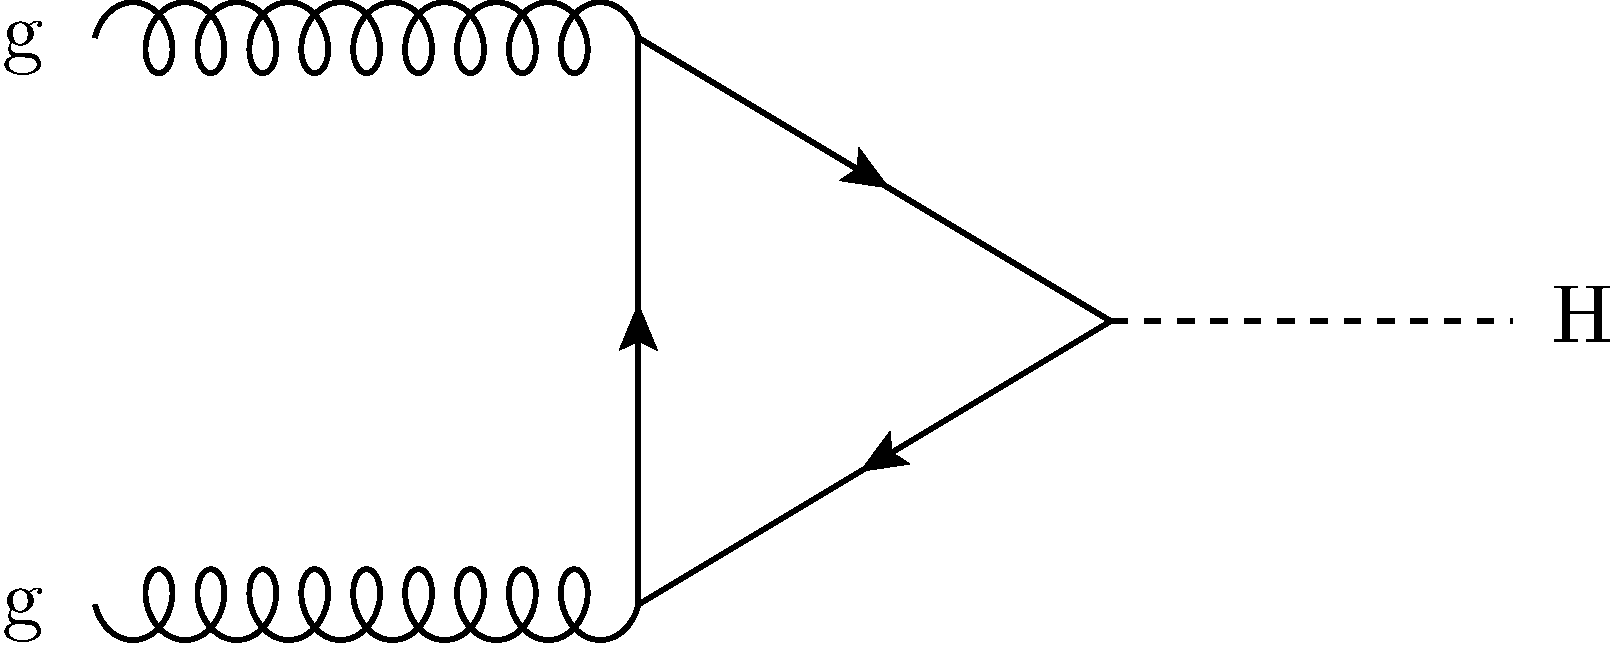
\includegraphics[width=0.5\textwidth]{./Theory/Figures/feynman_ggH.pdf}}
\subfloat[Vector boson fusion]{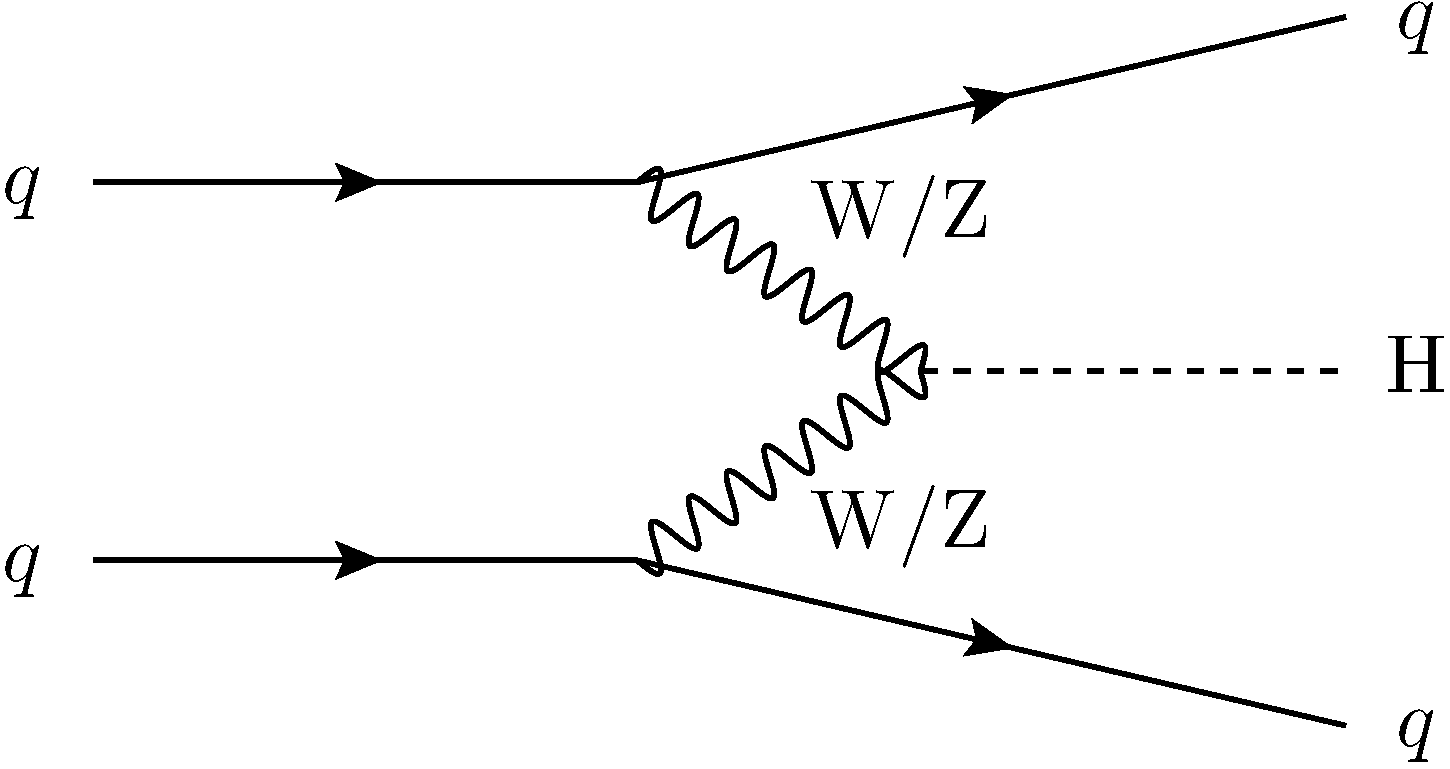
\includegraphics[width=0.5\textwidth]{./Theory/Figures/feynman_qqH.pdf}}~\\
\subfloat[W/Z associated production]{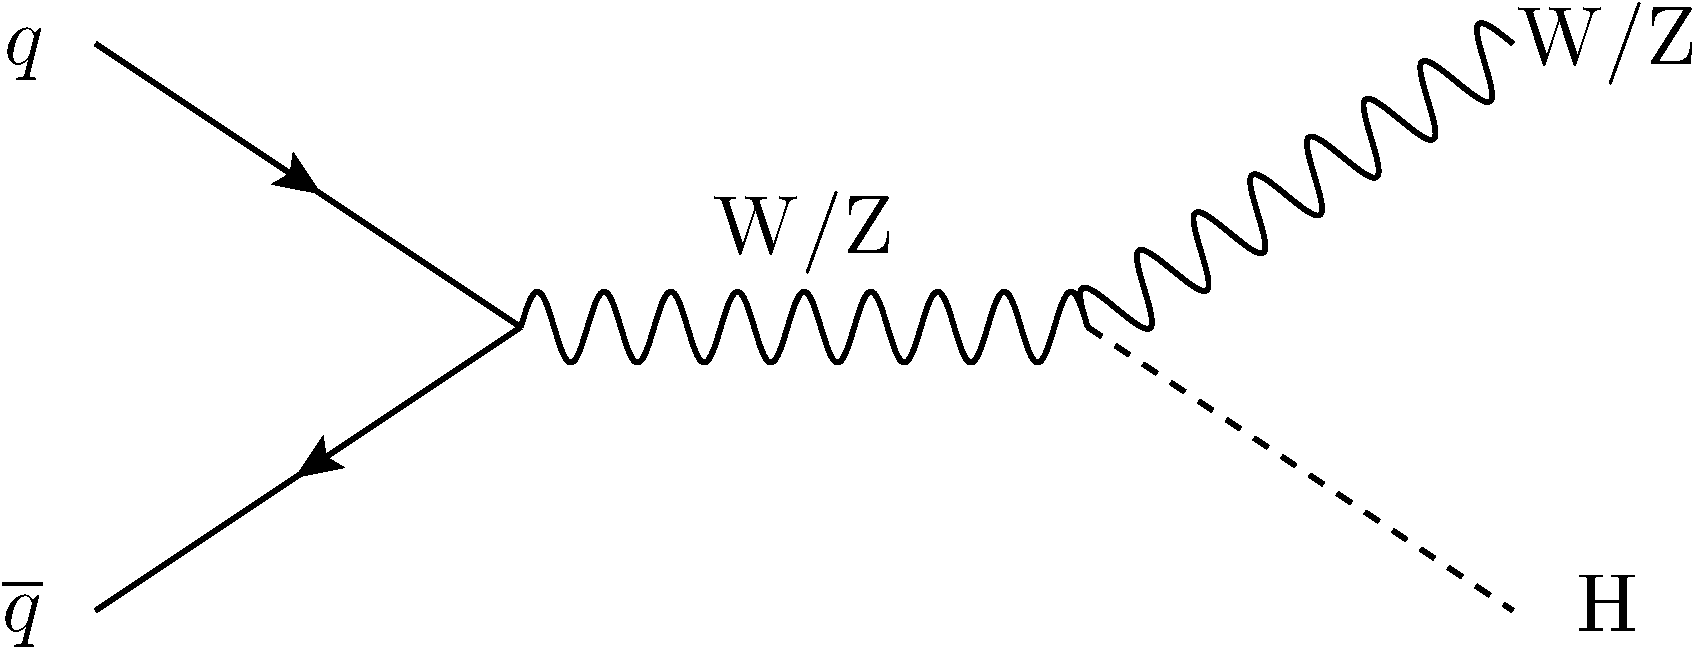
\includegraphics[width=0.5\textwidth]{./Theory/Figures/feynman_VH.pdf}}
\subfloat[\ttbar associated production]{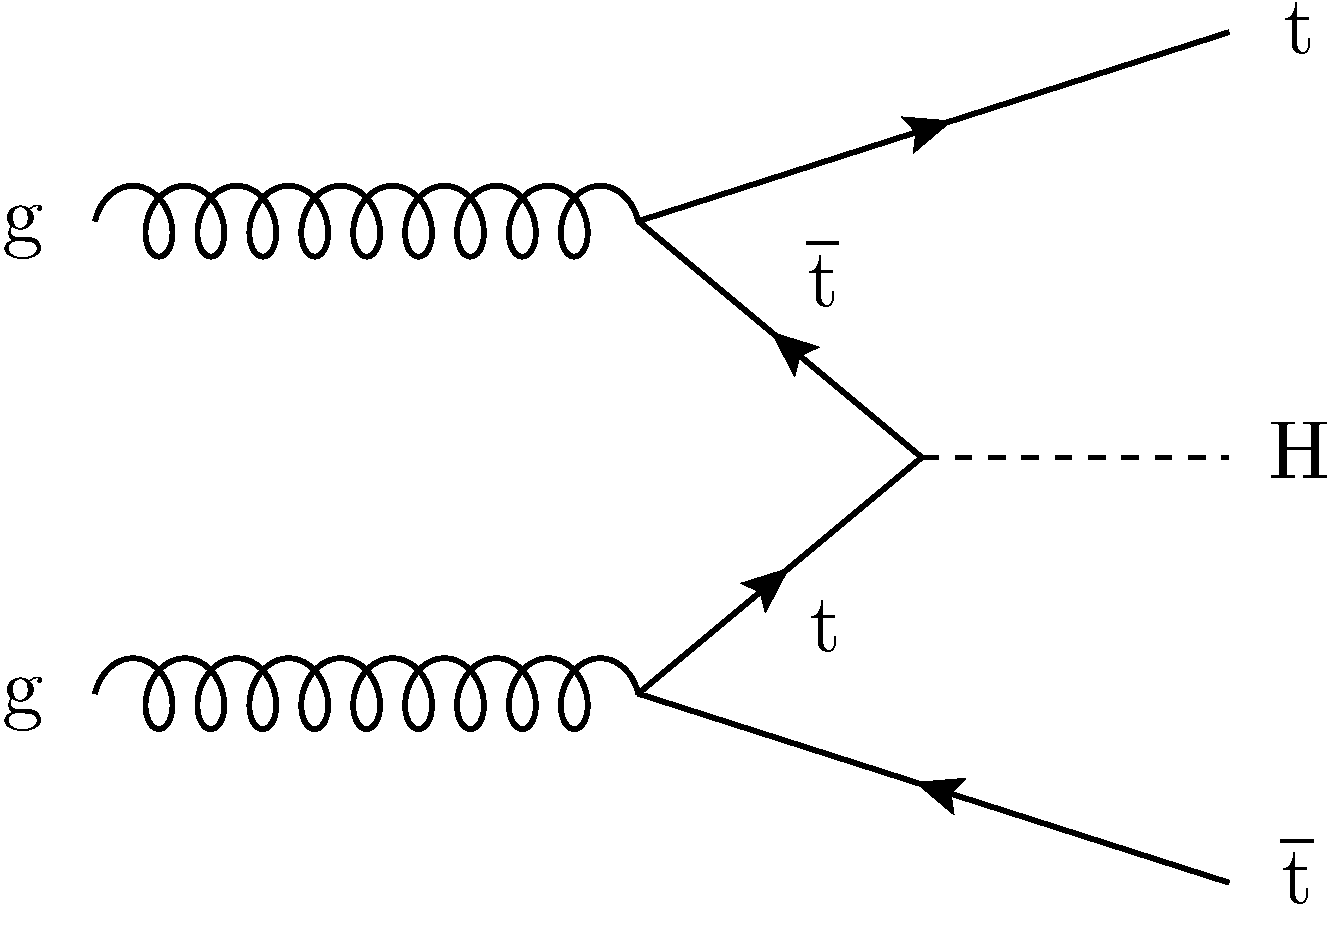
\includegraphics[width=0.5\textwidth]{./Theory/Figures/feynman_ttH.pdf}}
\end{center}
\caption[Tree-level Feynman diagrams for the dominant Higgs boson production modes at the LHC]{Tree-level Feynman diagrams for the dominant Higgs boson production modes at
the \ac{LHC}.}
\label{fig:theory_smhprod}
\end{figure}

Figure \ref{fig:theory_smhprod} shows Feynman diagrams of the dominant Higgs boson production modes
at the \ac{LHC}. The production cross sections for each mode, shown in figure
\ref{fig:theory_smhxsbr}a, show that gluon fusion production is by far dominant. The other modes
shown have cross sections at least an order of magnitude smaller, but are of importance due to their topologies.
Tagging the additional leptons or jets in the final states of
these production modes can reduce the size
of the \ac{SM} background.

\begin{figure}[h!]
\begin{center}
\subfloat[\ac{SM} Higgs boson production cross sections]{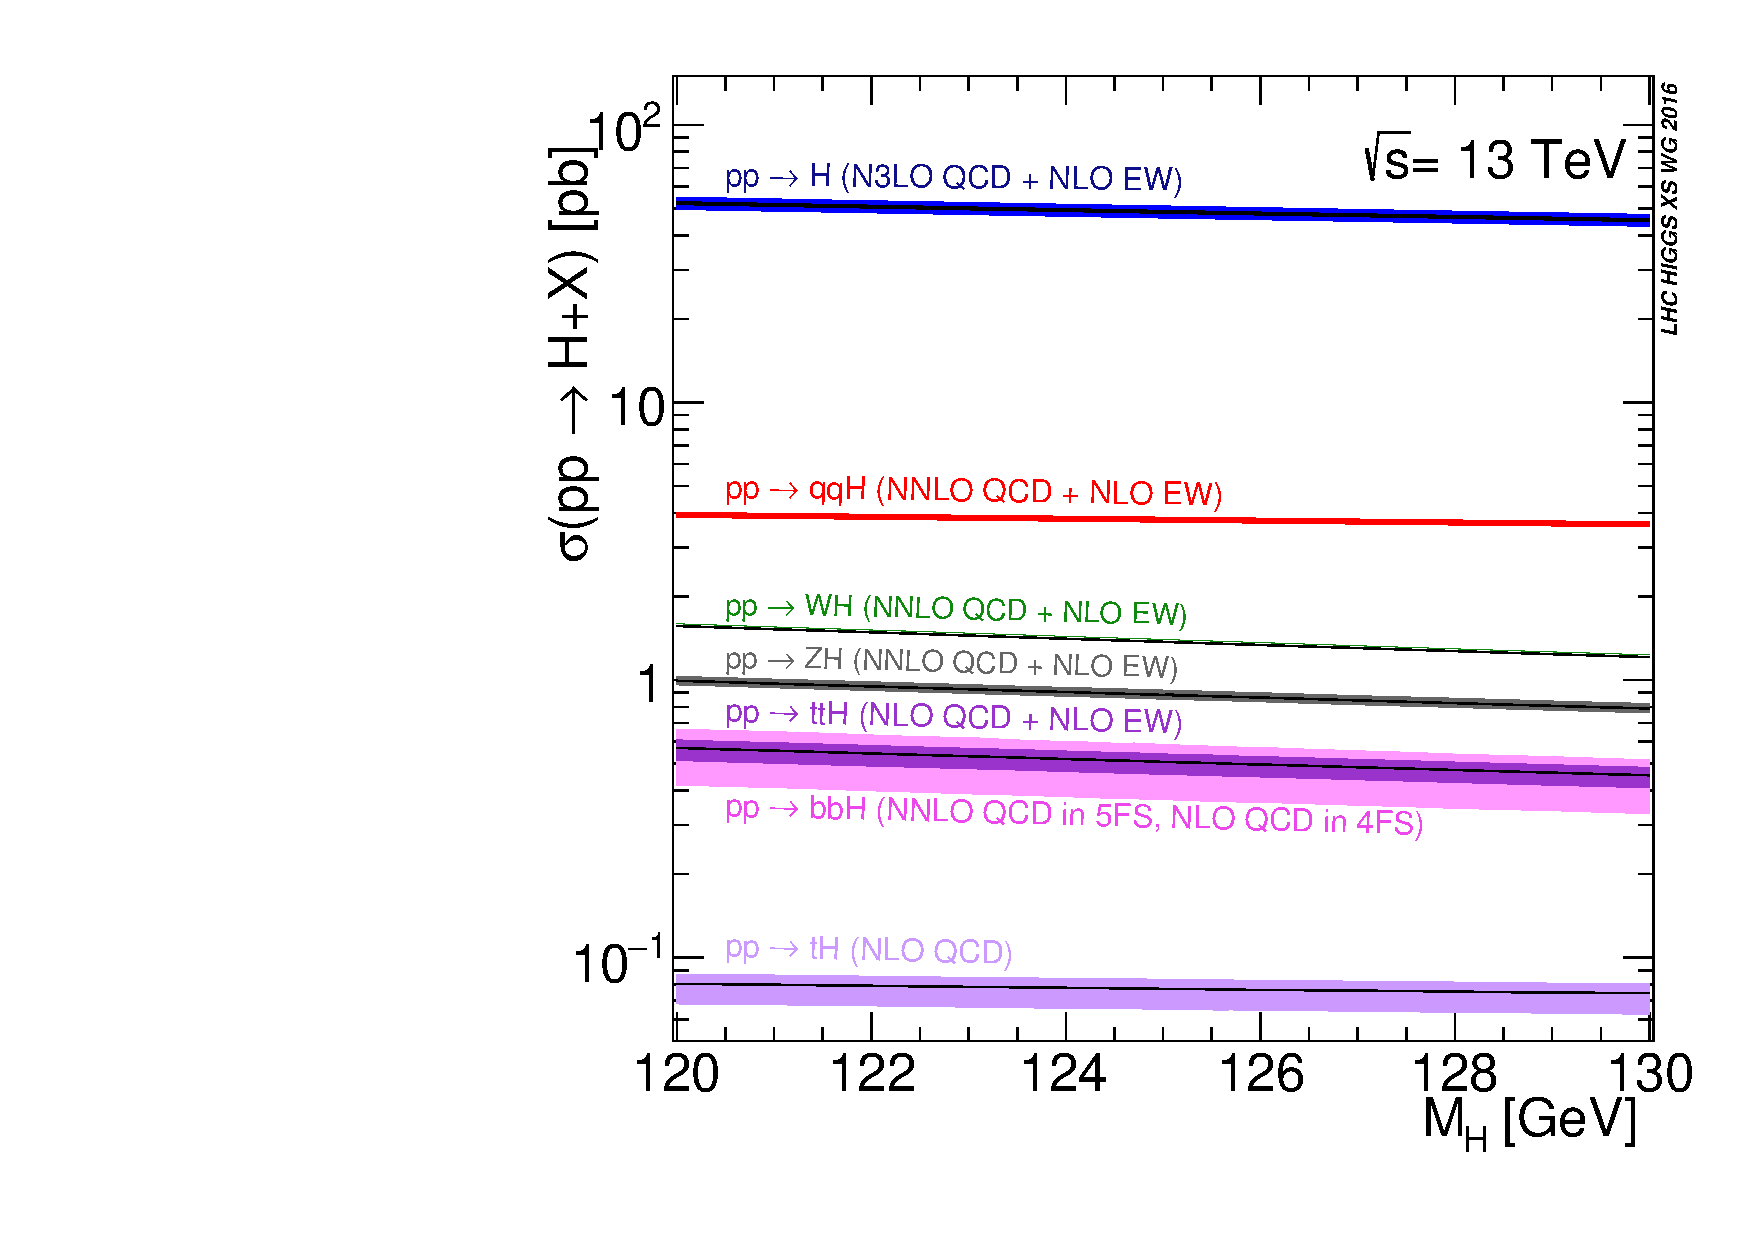
\includegraphics[width=0.5\textwidth]{./Theory/Figures/plot_13tev_H_sqrt.pdf}}
\subfloat[\ac{SM} Higgs boson branching ratios]{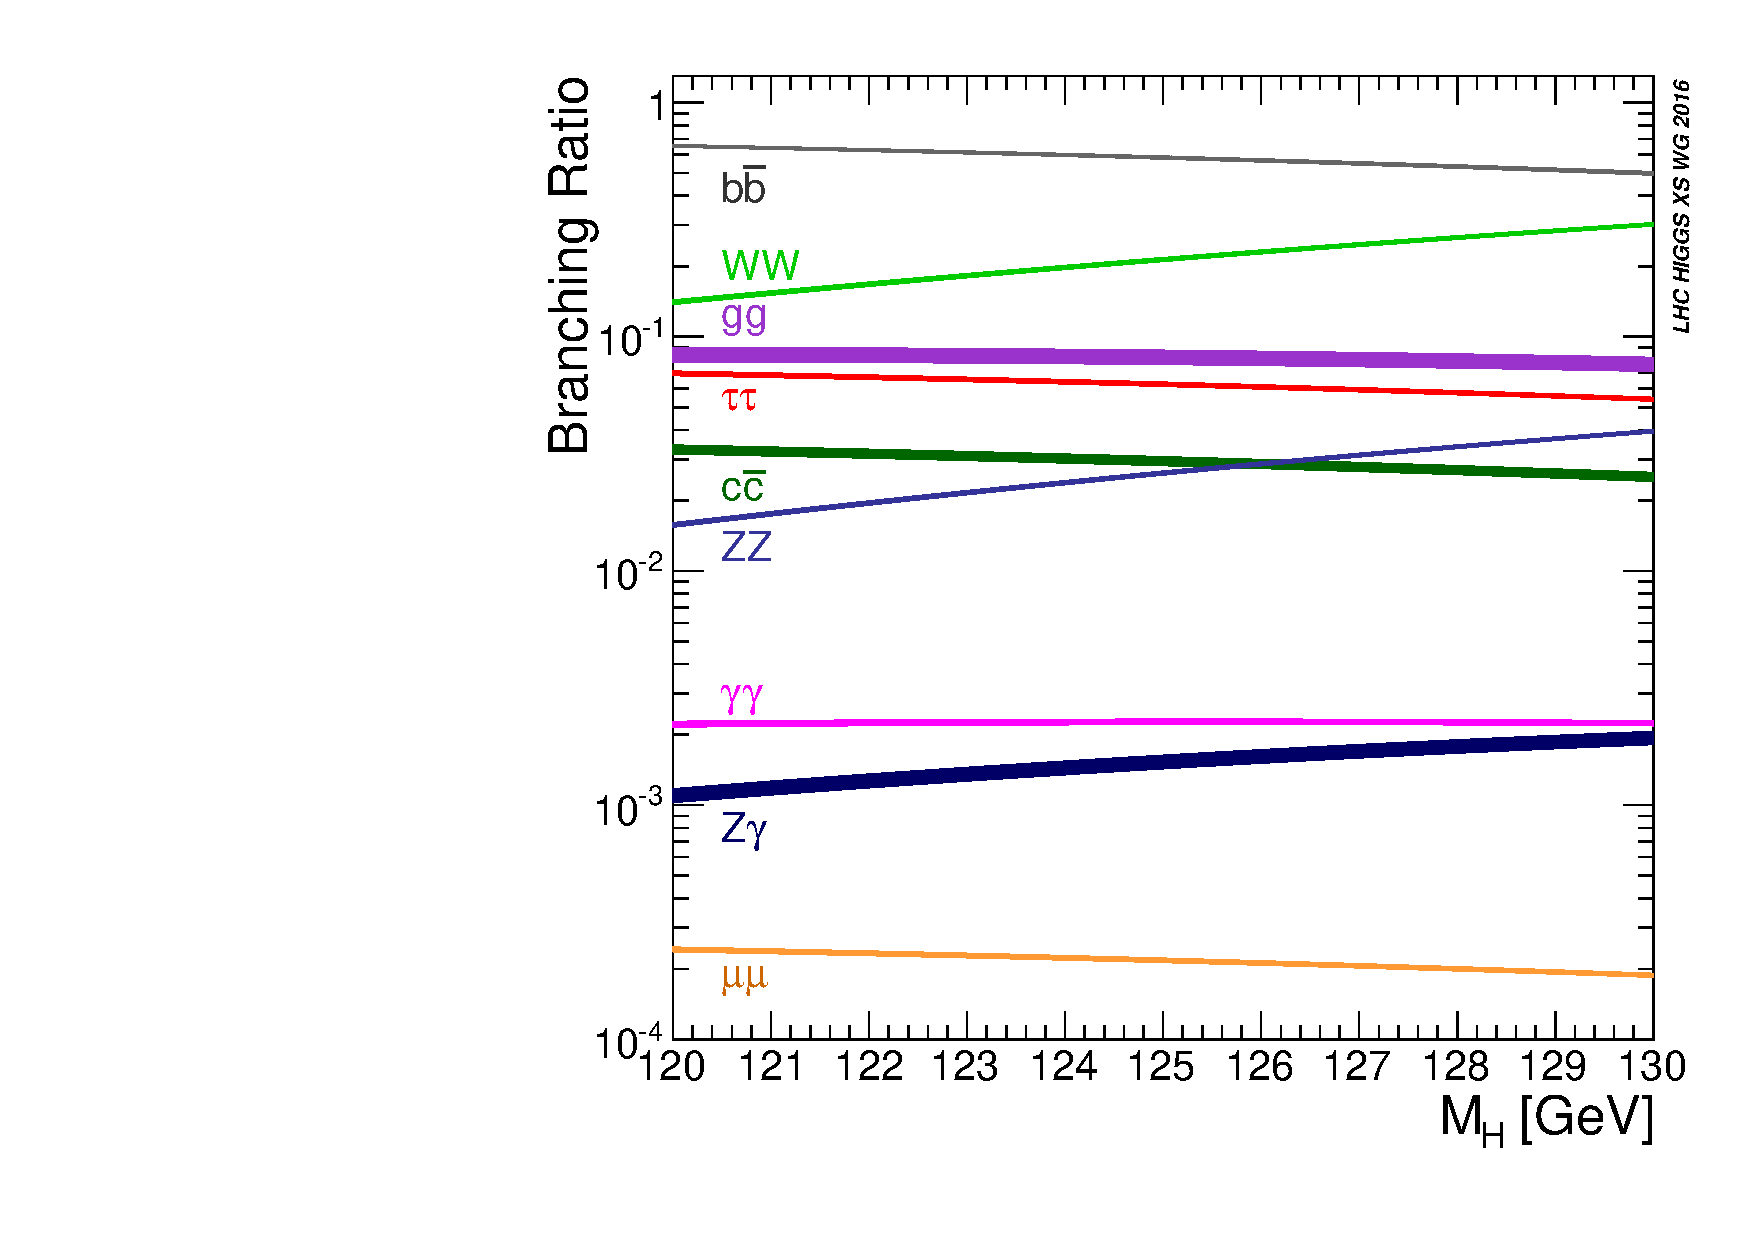
\includegraphics[width=0.5\textwidth]{./Theory/Figures/SMHiggsBRYR4-square.pdf}}
\end{center}
\caption[SM Higgs boson production cross sections at $\sqrt{s}=13\,\TeV$ and SM Higgs boson branching ratios, for Higgs boson masses between $120$ and $130\,\GeV$]{(a) \ac{SM} Higgs boson production cross sections at $\sqrt{s} = 13\,\TeV$ and (b) \ac{SM}
Higgs boson branching ratios, for Higgs boson masses between $120$ and $130\,\GeV$ \cite{YR4}.}
\label{fig:theory_smhxsbr}
\end{figure}

Figure \ref{fig:theory_smhxsbr}b shows that
the branching ratios of
$\PHiggs \rightarrow \gamma\gamma$ and $\PHiggs \rightarrow \PZ\PZ$, the two discovery
channels, are smaller than the branching ratios into many other final states.
These two channels are thus not sensitive as a result of the size of their branching ratios, but
rather due to the small backgrounds in these analyses as well as the excellent photon and lepton energy resolution the detectors provide.

Since the restart of the LHC in 2015, \ac{SM} Higgs boson measurements, and searches for the 
\ac{SM} Higgs boson in decay channels not previously established, have 
already been performed. The decay into $\gamma\gamma$ has been re-established \cite{CMSHgamgam2016,ATLASHgamgam2016},
as has the decay into $\PZ\PZ\rightarrow 4\ell$ \cite{CMSHZZ2016,ATLASHZZ2016}, and measurements
of $\PHiggs\rightarrow \PW\PW$ have been performed \cite{CMSHWW2016,ATLASHWW2016}. Establishing evidence for the decay of 
$\PHiggs\rightarrow \Pbottom\Pbottom$ \cite{CMSVBFHbb2016,ATLASVHbb2016} and of $\PHiggs\rightarrow \mu\mu$ \cite{ATLASHmm2016} 
is still to be achieved.
Finally, searches for $\Ptop\Ptop\PHiggs$ production, which are important to directly probe the top-Higgs coupling, have also been carried 
out \cite{CMSttH2016,CMSttHmultilep2016,ATLASttHbb2016,ATLASttHmultilep2016}. As more data
are collected studies at the \acs{LHC} will continue to test the compatibility of the Higgs boson with the \ac{SM}.

\section{Beyond the standard model}
\label{sec:theory_BSM}
The \ac{SM} has been successfully tested to high accuracy \cite{pdg-2014}. However,
some issues remain that cannot be addressed by the \ac{SM} alone \cite{griffiths}.
For example, it does not provide a candidate for dark matter, which is estimated
to make up 25\% of the matter-energy density in the universe.
In addition, the running coupling constants of the electroweak and
strong forces do not intersect at a common energy scale. Another problem is that the force
of gravity does not appear in the \ac{SM}.

These points aside, the most important issue concerning
the Higgs sector of the \ac{SM} is the hierarchy problem.
The \ac{SM}
is accepted to be an effective field theory that describes
the elementary particles and their interactions well, up to an energy scale $\Lambda$ beyond which it breaks down.
This is the energy scale at which new physics must enter.
It is known that $\Lambda \leq \mathcal{O}(10^{19})$, the Planck scale, as quantum 
gravitational effects start to become important in that region. The energy scale $\Lambda$ enters
the corrections due to fermion and boson loops to the Higgs boson mass quadratically \cite{MSSM-carena-haber}:
\begin{equation}\label{eqn:mh_hierarchy}
\begin{split}
&M_{\PHiggs_{\text{SM}}}^2  = (M_{\PHiggs})_0^2 + \Delta M_{\PHiggs}^2,\\
&\Delta M_{\PHiggs}^2 \sim \mathcal{O}(\Lambda^2).
\end{split}
\end{equation}
Thus assuming that there is no new physics all the way up to
the Planck scale the observation $M_{\PHiggs}=125\,\GeV$ would only be compatible with $\Lambda$ of order $10^{19}\,\GeV$
if there was extreme fine-tuning of the bare Higgs boson mass $(M_{\PHiggs})_0^2$.

Many \acf{BSM} theories that can address the hierarchy problem, and some of
the other issues that were mentioned, have been developed.
One of the most
popular of these theories is \acf{SUSY} \cite{SUSY-primer}, which postulates
that there is a symmetry between bosons and fermions. This means every fermionic
\ac{SM} particle has a bosonic superpartner (sfermion, for scalar fermion)
and every bosonic \ac{SM} particle
has a fermionic superpartner (boson name + `ino', e.g. higgsino, Wino).

If this symmetry is unbroken the \ac{SUSY} particles must
have the same mass as their \ac{SM} partners. However, if that had 
been the case such particles would have been detected a long time ago. The 
only possibility is then that \ac{SUSY} is a broken symmetry and the superpartners
are heavier than their \ac{SM} equivalents. It is important to note
that the fermion and boson loops contribute to the Higgs boson
mass corrections with opposite sign, and so the symmetry between bosons and fermions 
allows for the cancellation of $\Delta M_{\PHiggs}^2$ terms. The cancellation
would be exact if \ac{SUSY} were unbroken, but because this is not the case the
cancellation is not complete. Therefore if the \ac{SUSY} breaking scale, where
new particles should be found, is much larger than a few TeV further fine-tuning of
the bare Higgs boson mass would be required \cite{MSSM-carena-haber,SUSY-primer}.
Apart from solving the hierarchy problem, \ac{SUSY} addresses some
of the other aforementioned issues. The lightest \ac{SUSY} particle
would be a candidate for dark matter if it were stable \cite{SUSY-primer}. On top of that,
\ac{SUSY} allows the electroweak and strong coupling
constants to intersect at a common energy scale of $\mathcal{O}(10^{16}\,\GeV)$ \cite{GUT-LEP}. 

The simplest supersymmetric extension of the \ac{SM}, the \ac{MSSM} \cite{SUSY-primer}, only adds the minimum
number of particles and fields required to formulate a supersymmetric theory.
%And conserves R-parity, see section 6.2 of the SUSY primer

\subsection{The Higgs sector of the \acs{MSSM}}
\label{sec:theory_MSSM_H}
At least two Higgs doublets are required in the
Higgs sector of the \ac{MSSM}, and so in its simplest form two complex Higgs doublets are added \cite{MSSM-carena-haber},
\begin{equation}\label{eqn:mssm_higgsdoublets}
\Phi_d = \begin{pmatrix} \phi_d^0 \\
\phi_d^- \end{pmatrix} \text{ and } \Phi_u = \begin{pmatrix} \phi_u^+ \\
\phi_u^0 \end{pmatrix}.
\end{equation}
Note that $\phi_d^0$ couples exclusively to down-type fermions, and $\phi_u^0$ couples
exclusively to up-type fermions.
%This leads to potential terms in the MSSM Lagrangian of the form:
%\begin{equation}\label{eqn:mssm_lagrangian_potential}
%V = \mu(\phi_u^+\phi_d^- - \phi_u^0\phi_d^0),
%\end{equation}
%with $\mu$ a mass parameter, equivalent to the \ac{SM} Higgs mass parameter.
Electroweak symmetry is broken as in the \ac{SM} case and
minimising the potential associated with the two Higgs doublets gives,
\begin{equation}\label{eqn:mssm_minimpot}
\langle 0|\Phi_d| 0 \rangle = \begin{pmatrix}v_d\\
0 \end{pmatrix} \text{ and } \langle 0 |\Phi_u|0\rangle  = \begin{pmatrix} 0\\
v_u \end{pmatrix}.
\end{equation}
This can be used to define
\begin{equation}\label{eqn:tanb_def}
\tan{\beta} \equiv \frac{v_u}{v_d}.
\end{equation}
Of the eight degrees of freedom due to the introduction of two complex
doublets, three become longitudinal states of the $\PW^{\pm}$ and \PZ bosons.
The remaining five degrees of freedom lead to five physical Higgs bosons: a charged
Higgs boson pair $\PHiggs^{\pm}$, the neutral pseudoscalar \PHiggsps
and the neutral scalars \PHiggslight and \PHiggs. These arise from the mixing of the
fields as:
\begin{align}\label{eqn:MSSMHiggsMixing}
&\PHiggs^+ = \phi_u^+\cos{\beta} + \phi_d^{-\dagger}\sin{\beta},\\
&\PHiggs^- = \phi_u^{+\dagger}\cos{\beta} + \phi_d^{-}\sin{\beta},\\
&\PHiggsps = \sqrt{2}(\text{Im}\phi_d^0\sin{\beta} + \text{Im}\phi_u^0\cos{\beta}),\\
&\PHiggslight = -(\sqrt{2}\text{Re}\phi_d^0 - v_d)\sin{\alpha} + (\sqrt{s}\text{Re}\phi_u^0 -v_u)\cos{\alpha},\\
&\PHiggs = (\sqrt{2}\text{Re}\phi_d^0-v_d)\cos{\alpha}+(\sqrt{2}\text{Re}\phi_u^0-v_u)\sin{\alpha}.
\end{align}
These mixtures depend on \tanb~and the mixing angle $\alpha$ which is found
by diagonalising
the neutral scalar Higgs squared-mass matrix,
\begin{equation}\label{eqn:treelevel_mass}
\mathcal{M}_{\text{tree}}^2 = \begin{pmatrix} 
m_{\PHiggsps}^2\sin{\beta}^2 + m_{\PZ}^2\text{cos}^2\beta & -(m_{\PHiggsps}^2+m_{\PZ}^2)\sin{\beta}\cos{\beta}\\
-(m_{\PHiggsps}^2+m_{\PZ}^2)\sin{\beta}\cos{\beta} & m_{\PHiggsps}^2\text{cos}^2\beta+m_{\PZ}^2\text{sin}^2{\beta} \end{pmatrix},
\end{equation}
of which \PHiggs and \PHiggslight are the eigenstates.
As the self-interactions of the Higgs fields are not independent parameters,
%they are functions of the electroweak gauge coupling constants 
at tree level the MSSM Higgs sector is determined by two free parameters, \tanb~and
one of the Higgs boson masses, conventionally chosen as \mA.
The masses of the neutral scalars \PHiggs and \PHiggslight are the eigenvalues  
of $\mathcal{M}_{\text{tree}}^2$,
\begin{equation}\label{eqn:scalarmass}
m_{\PHiggs,\PHiggslight}^2 = \frac{1}{2}[m_{\PHiggsps}^2+m_{\PZ}^2 \pm \sqrt{(m_{\PHiggsps}^2+m_{\PZ}^2)^2-4m_{\PZ}^2m_{\PHiggsps}^2\text{cos}^2 2\beta}~].
\end{equation}
The masses of the charged Higgs bosons are
\begin{equation}\label{mssm_chargedhigss_mass}
m_{\PHiggs^{\pm}}^2 = m_{\PHiggsps}^2+m_{\PW}^2.
\end{equation}
%while the neutral scalar \PHiggslight and \PHiggs are eigenstates of the
%squared-mass matrix at tree level:
%\begin{equation}\label{eqn:treelevel_mass}
%\mathcal{M}_{\text{tree}}^2 = \begin{pmatrix} 
%m_{A}^2\sin{\beta}^2 + m_{Z}^2\cos{\beta}^2 & -(m_{A}^2+m_{Z}^2)\sin{\beta}\cos{\beta}\\
%-(m_{A}^2+m_{Z}^2)\sin{\beta}\cos{\beta} & m_{A}^2\cos{\beta}^2+m_{Z}^2\sin{\beta}^2 \end{pmatrix}.
%\end{equation}
%Such that $m_{\PHiggs,\PHiggslight}$ are eigenvalues of $\mathcal{M}_{\text{tree}}^2$,
%\begin{equation}\label{eqn:scalarmass}
%m_{\PHiggs,\PHiggslight}^2 = \frac{1}{2}(m_{A}^2+m_{Z}^2 \pm \sqrt{(m_A^2+m_Z^2)^2-4m_Z^2m_A^2\cos{2\beta}^2}).
%\end{equation}
A consequence of equation \ref{eqn:scalarmass} is a tree-level upper bound on the mass of the light Higgs
boson,
\begin{equation}\label{eqn:mh_upper}
m_{\PHiggslight} \leq m_{\PZ},
\end{equation}
and a constraint on $\alpha$,
\begin{equation}\label{eqn:alpha_constraint}
\text{cos}^2(\beta-\alpha) = \frac{m_{\PHiggslight}^2(m_{\PZ}^2-m_{\PHiggslight}^2)}{m_{\PHiggsps}^2(m_{\PHiggs}^2-m_{\PHiggslight}^2)}.
\end{equation}

The requirement that $m_{\PHiggslight}$ be less than the mass of the \PZ boson, $91.2\,\GeV$, seems 
problematic at first, as it is known that there is a Higgs state with a mass of $125\,\GeV$. However,
the tree-level masses and couplings of the Higgs bosons in the \ac{MSSM} can be
significantly altered by radiative corrections. The dominant effect is from
incomplete cancellation of the stop- and top-loop corrections. This can increase the mass
of the light Higgs boson up to a maximum of $135\,\GeV$.

The tree-level couplings of the neutral Higgs bosons to bosons and fermions 
are modified with respect to the couplings of the Higgs boson in the \ac{SM} by the multiplicative factors
given in table \ref{tab:mssm_couplings} \cite{YR4}.
\begin{table}[htp]
\label{tab:mssm_couplings}
\begin{center}
\caption[Tree-level couplings in the MSSM, as multiplicative factors with respect to the couplings of the Higgs boson in the SM.]{Tree-level couplings in the MSSM, as multiplicative factors with
respect to the couplings of the Higgs boson in the \ac{SM}.}
\begin{tabular}{p{2cm}p{4cm}p{4cm}p{4cm}}
\toprule
Particle & Coupling to bosons & Coupling to up-type quarks & Coupling to down-type quarks and leptons \\
\midrule
\PHiggsps & 0 & $\cot{\beta}$ & $ \tan{\beta}$\\
\PHiggs & $\cos{(\beta-\alpha)}$ & $\frac{\sin{\alpha}}{\sin{\beta}}$ & $\frac{\cos{\alpha}}{\cos{\beta}}$\\
\PHiggslight & $\sin{(\beta-\alpha)}$ & $\frac{\cos{\alpha}}{\sin{\beta}}$ & $-\frac{\sin{\alpha}}{\cos{\beta}}$\\
\bottomrule
\end{tabular}
\label{tab:mssm_couplings}
\end{center}
\end{table}

In the \textit{decoupling limit}, when $m_{\PHiggsps} \gg m_{\PZ}$ and $\cos{(\beta-\alpha)}$ tends
to zero, the mixing
angle $\alpha \approx \beta - \pi/2$. This reduces the couplings in table
\ref{tab:mssm_couplings} to the \ac{SM} couplings for the \PHiggslight boson, 
with negligible couplings to bosons for the two remaining neutral
Higgs bosons; couplings to down-type quarks and leptons enhanced by a factor \tanb;
and couplings to up-type quarks enhanced by a factor $\frac{1}{\tan{\beta}}$. This motivates
the choice of decay into $\Pgt\Pgt$ as a search channel for the neutral Higgs bosons in the \ac{MSSM}.
Figure \ref{fig:mssm_brtautau} shows the branching ratios of the \PHiggs boson 
in the $m_{\PHiggslight}^{\text{mod+}}$ scenario
which will be discussed in more detail in section \ref{sec:theory_BSM_models_mhmodp}. 
The branching ratio into di-tau pairs is large for \tanb~$= 30$. The branching ratios 
 of the \PHiggsps boson follow a similar pattern.
%Using trigon identities: cos alpha/cos beta = cos (beta-pi/2)/cos beta = cosbeta*cospi/2 + sin(beta)*sin(pi/2) over cos beta = sin beta /cos beta = tan beta
%sin alpha = sin (beta-pi/2) = sinbeta cos pi/2 - cosbetasinpi/2 = -cosbeta 
%such that -sinalpha/cosbeta = 1
%cos alpha/sin beta = sin beta/sin beta = 1
%sin beta-alpha = sin pi/2 = 1
%cos beta-alpha = cos pi/2 = 0
%sin alpha/sin beta = -cos beta/sin beta=-1/tan(beta)

\begin{figure}[h!]
\begin{center}
\subfloat[\tanb=5]{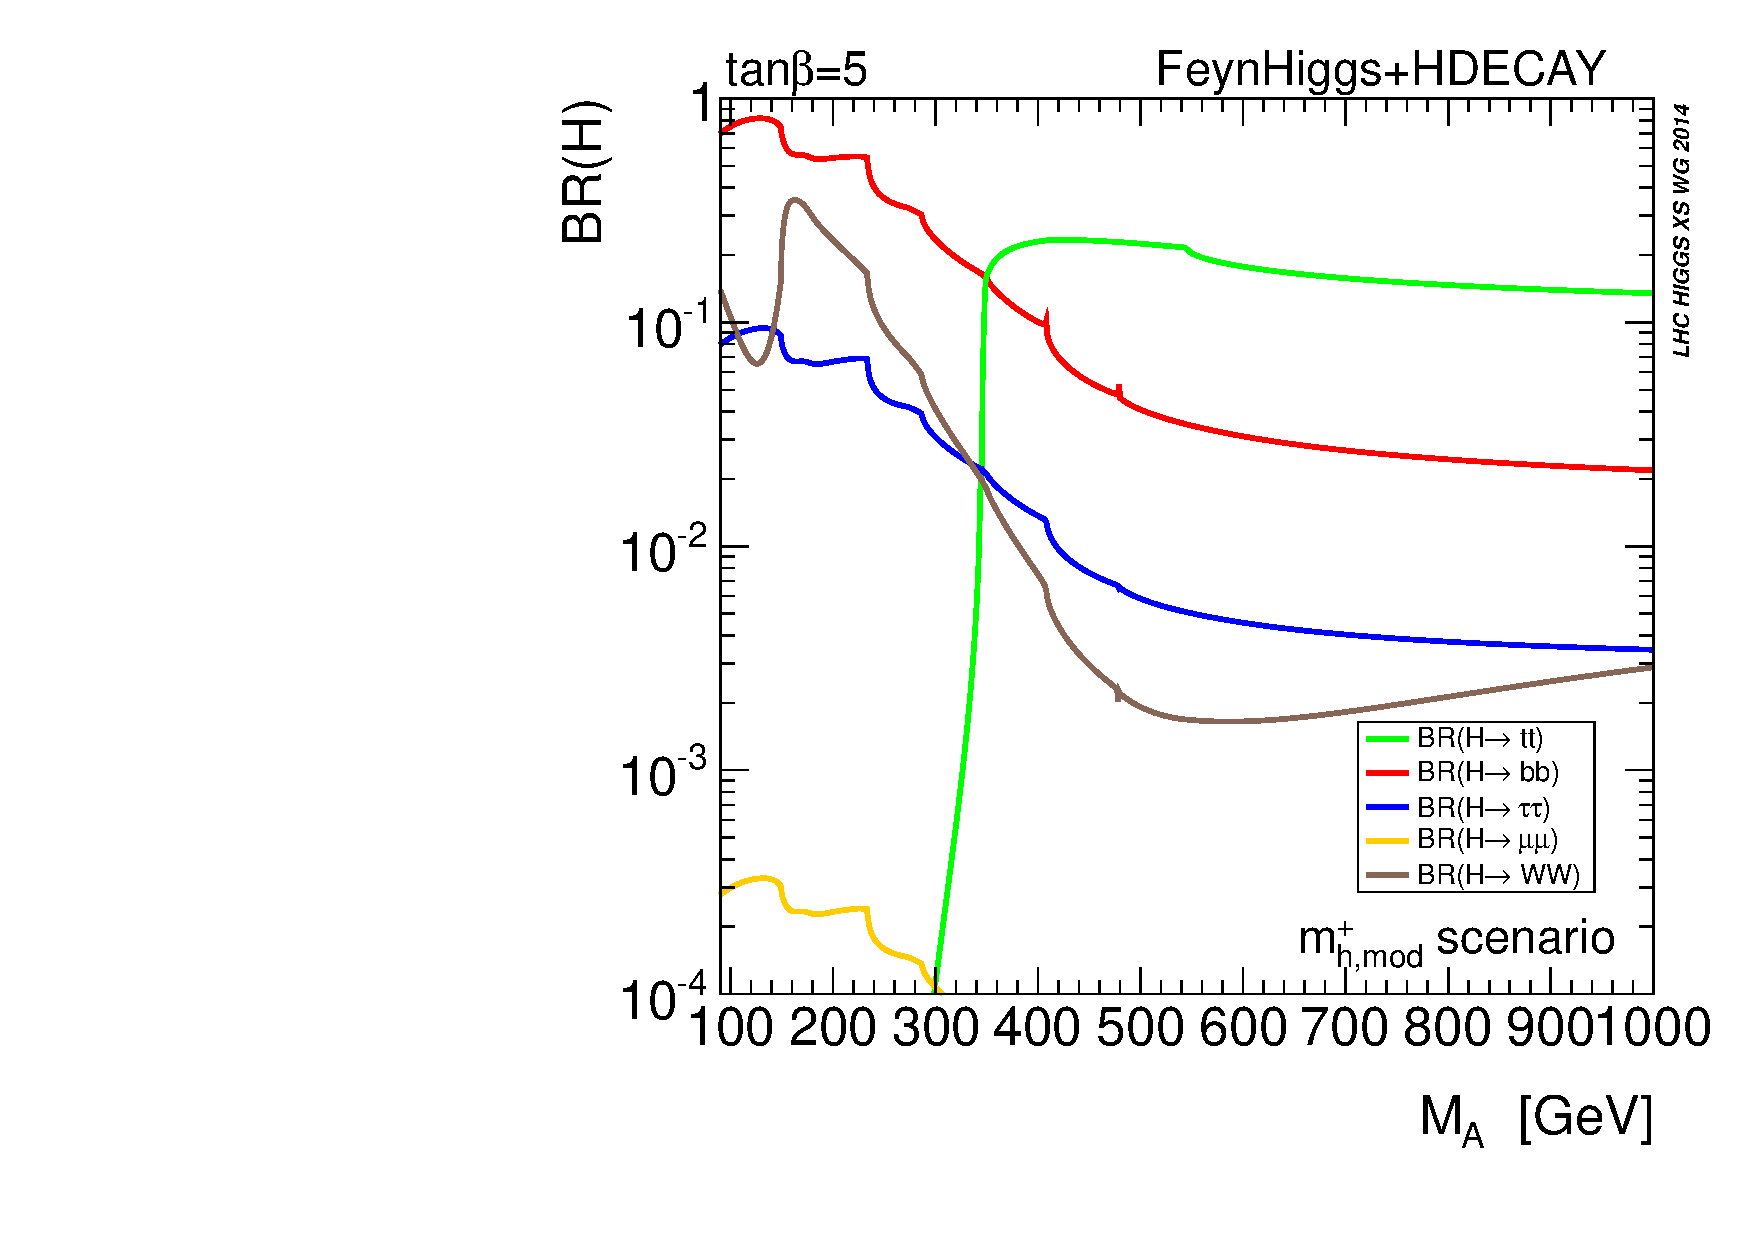
\includegraphics[width=0.5\textwidth]{./Theory/Figures/YR4HXS_BRSummary_H_mhmodp_tanbeta5_FeynHiggs_HDecay.pdf}}
\subfloat[\tanb=30]{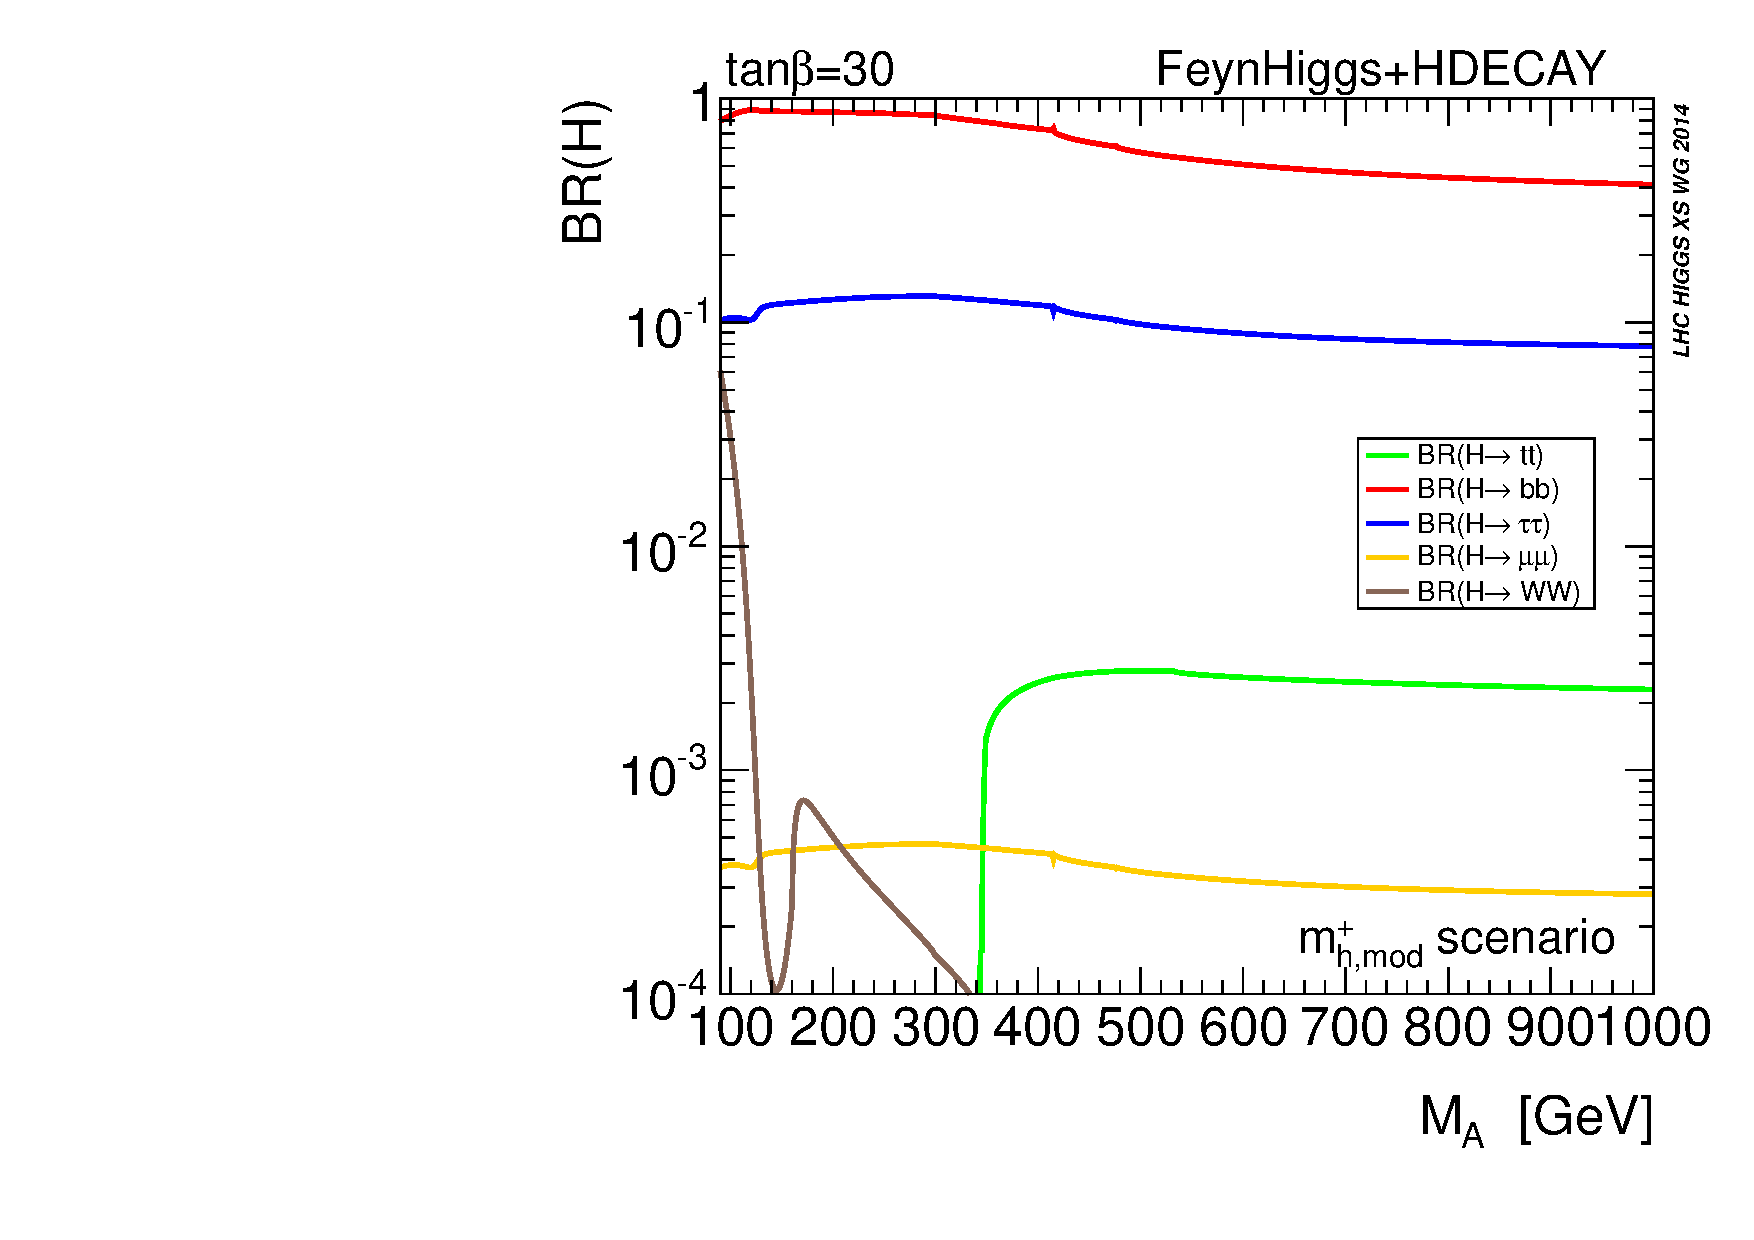
\includegraphics[width=0.5\textwidth]{./Theory/Figures/YR4HXS_BRSummary_H_mhmodp_tanbeta30_FeynHiggs_HDecay.pdf}}
\end{center}
\caption[Branching ratios of the \PHiggs boson in the $m_{\PHiggslight}^{\text{mod+}}$ scenario]{Branching ratios of the \PHiggs boson in the $m_{\PHiggslight}^{\text{mod+}}$ scenario,
at (a) \tanb=5~and (b) \tanb=30. The branching ratio into $\tau\tau$ (blue), $\Pbottom\APbottom$ (red) 
and $\mu\mu$ (yellow) is enhanced at high \tanb, while the branching ratio into 
WW (brown) and \ttbar (green) is reduced \cite{MSSM-xswg-twiki}.}
\label{fig:mssm_brtautau}
\end{figure}

The dominant neutral MSSM Higgs boson production processes at hadron colliders
are slightly different from the \ac{SM} Higgs boson production processes. 
Because the pseudoscalar A does not couple to the
vector bosons, and in the decoupling limit the coupling of \PHiggs to vector
bosons is suppressed with respect to the \ac{SM} expectation, \ac{VBF} and \PW or \PZ associated
production ($\PW\PHiggs$ or $\PZ\PHiggs$) are not as important as for the production of the \ac{SM} Higgs boson. As in the \ac{SM}, gluon fusion production is 
the dominant production mode at low \tanb.
An example tree-level Feynman diagram for gluon fusion production, which proceeds via
a quark loop, is given in figure \ref{fig:production_mssm}a.
At low \tanb~values this loop is dominated by top quarks, while at 
high \tanb~the b-quark loop dominates. This is a result of the enhanced coupling to down-type fermions at high \tanb. 
Due to the negative top-bottom loop interference effect the gluon fusion cross section decreases with increasing \tanb~up
to around \tanb~$=3$, where the cross section starts to increase with increasing \tanb~again.

Another consequence of the enhanced couplings to down-type fermions at high \tanb~is the dominance of b-associated production, where the Higgs boson is produced through
bottom quark fusion. The tree-level Feynman diagram for this process is shown in figure \ref{fig:production_mssm}b.

\begin{figure}[h!]
\begin{center}
\subfloat[Gluon fusion production]{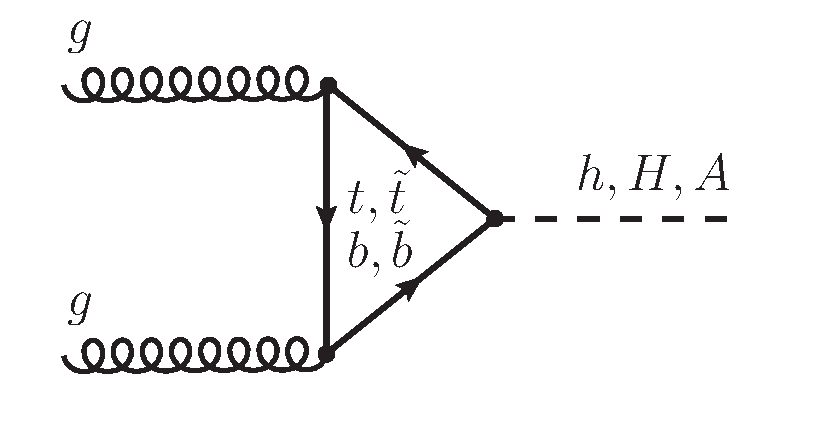
\includegraphics[width=0.5\textwidth]{./Theory/Figures/CMS-PAS-HIG-16-037_Figure_001-a.pdf}}
\subfloat[b-Associated production]{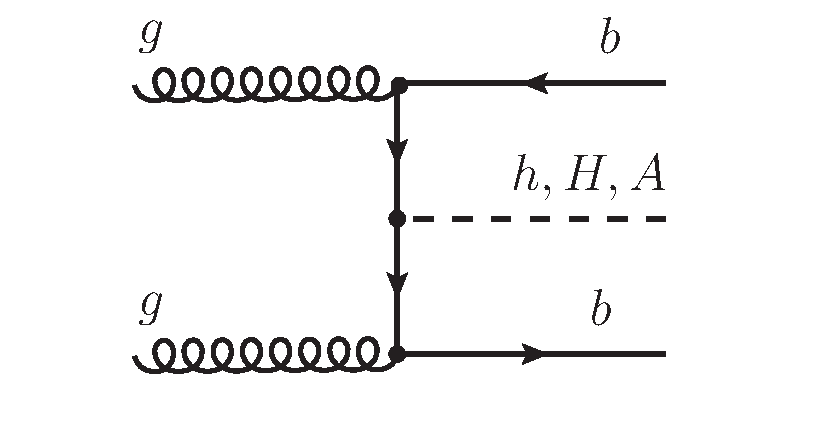
\includegraphics[width=0.5\textwidth]{./Theory/Figures/CMS-PAS-HIG-16-037_Figure_001-b.pdf}}
\end{center}
\caption[Tree-level Feynman diagrams of gluon fusion and b-associated production of neutral Higgs bosons in the MSSM]{Tree-level Feynman diagrams of (a) gluon fusion production and (b) b-associated
production of neutral Higgs bosons in the MSSM. The squarks in the gluon fusion production loop do not contribute to the production of the \PHiggsps boson.}
\label{fig:production_mssm}
\end{figure}

\subsection{Two Higgs doublet models}
\label{sec:theory_2HDM}
A different approach, also leading to an extended Higgs sector with
respect to the \ac{SM}, is found in \acp{2HDM} \cite{2HDM-I,2HDM-II}.
As the name suggests \acp{2HDM} are a generic class of models in which
there is not one, but two Higgs doublets. The addition of a second
Higgs doublet can not just be motivated by \ac{SUSY}, but also by other models.
An important point is that despite the presence of a second 
Higgs doublet, there are no explicit \ac{SUSY} particles in the \ac{2HDM}.

There are several different types of \ac{2HDM}, all distinguished by the couplings
of the different Higgs states to bosons and fermions. In its most general
form, there are nine free parameters in the potential of a CP-conserving 2HDM. 
These are taken as \tanb~and the mixing angle $\alpha$, already discussed in 
the context of the \ac{MSSM}, the masses of the five Higgs bosons,
and quartic couplings appearing in the potential. The most studied of the
\ac{2HDM}s, the type-II \ac{2HDM}, has a structure very similar to 
the MSSM Higgs sector. The tree-level couplings of the neutral Higgs bosons to 
vector bosons and fermions are the same as the tree-level \ac{MSSM} couplings 
in table \ref{tab:mssm_couplings}. %The decay \AtoZh is also possible,
%the \AtoZh~coupling is proportional to $\cos{(\beta-\alpha)}, like the \Htohh~coupling.

The behaviour of the \ac{2HDM} couplings in the \textit{alignment limit},
where $\cos{(\beta-\alpha)} = 0$, differs from that of the \ac{MSSM} couplings.
In particular, in the alignment limit of the \ac{2HDM} the decays \AtoZh~and \Htohh~vanish.
This is due to the fact that these couplings are
proportional to $\cos{(\beta-\alpha)}$ and there are no corrections
from \ac{SUSY} particles to make the branching ratios non-zero.

The inclusive cross section times branching ratio (\xsbr) for production of an \PHiggs boson 
and decays into various final states is shown in figure \ref{fig:2hdm_Hxsbr}a for an 
example of a type-II \ac{2HDM}, for two values of \tanb. Figure \ref{fig:2hdm_Hxsbr}b 
shows the inclusive \xsbr for production and decay
of an \PHiggsps boson in the same type-II \ac{2HDM} example, at two values of \tanb. At
low \tanb~the \xsbr for \Htohh production and decay and \AtoZh production
and decay are enhanced for $250\leq m_{\PHiggs}\leq 350\,\GeV$ and $220 \leq m_{\PHiggsps} \leq 350\,\GeV$, respectively.

\begin{figure}[h!]
\begin{center}
\subfloat[\PHiggs boson]{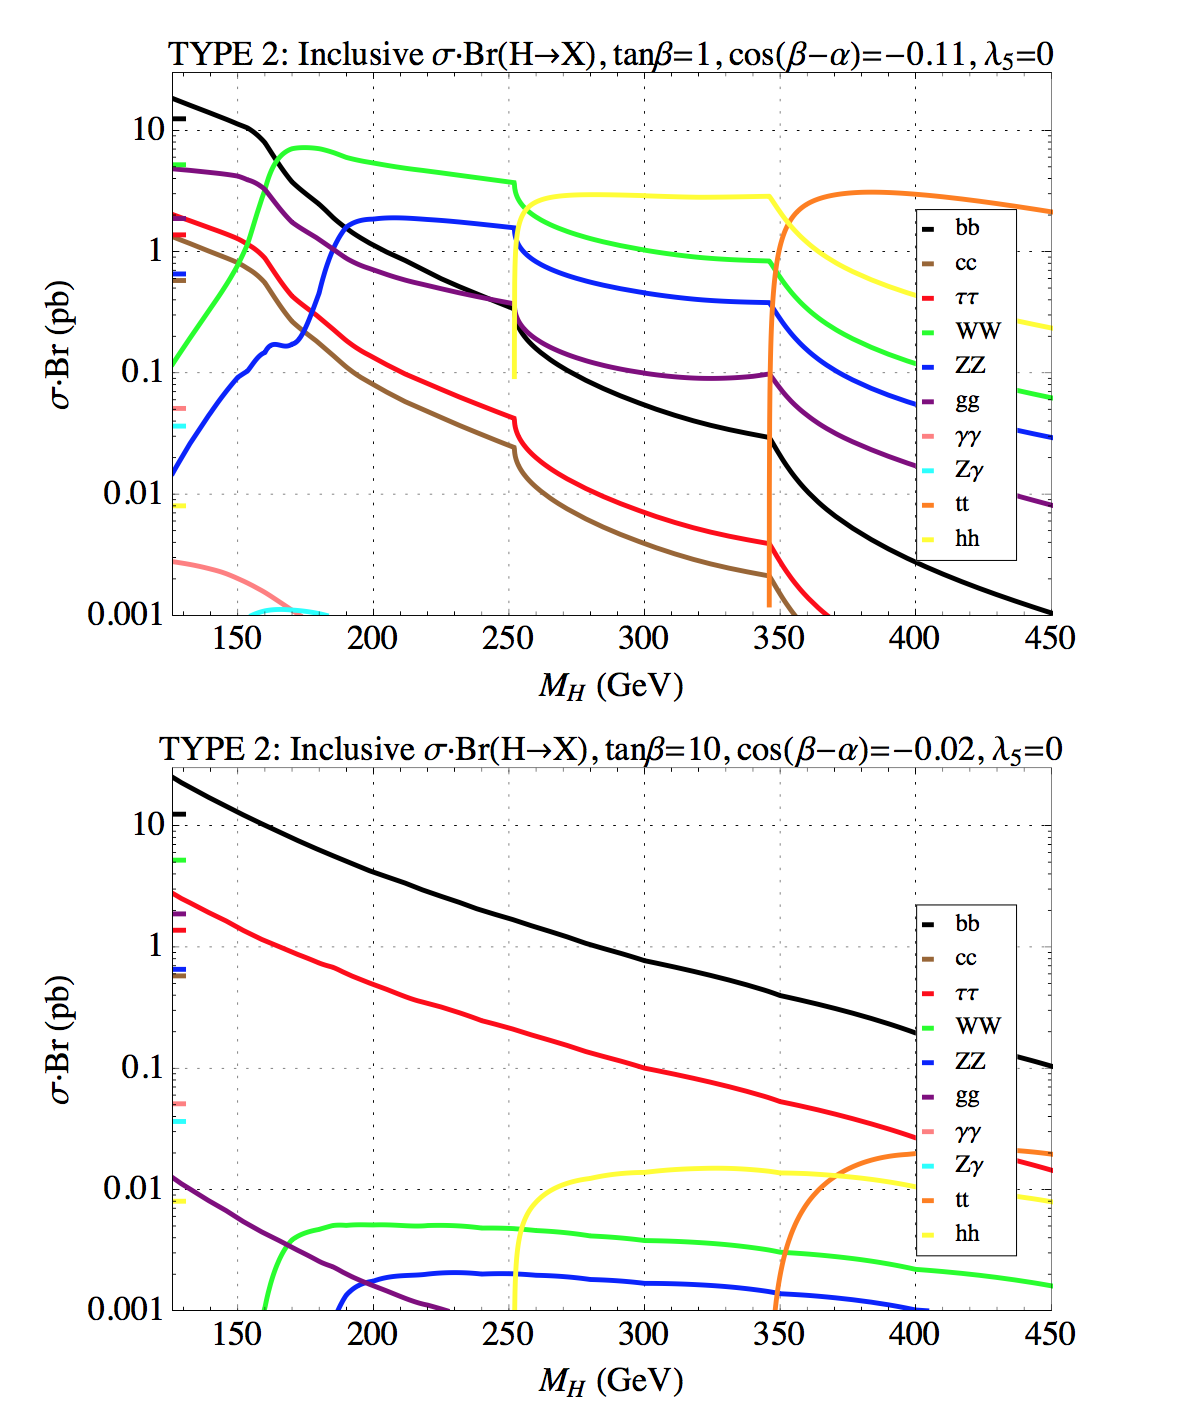
\includegraphics[width=0.516\textwidth]{./Theory/Figures/typeII2HDMxsbr.png}}
\subfloat[\PHiggsps boson]{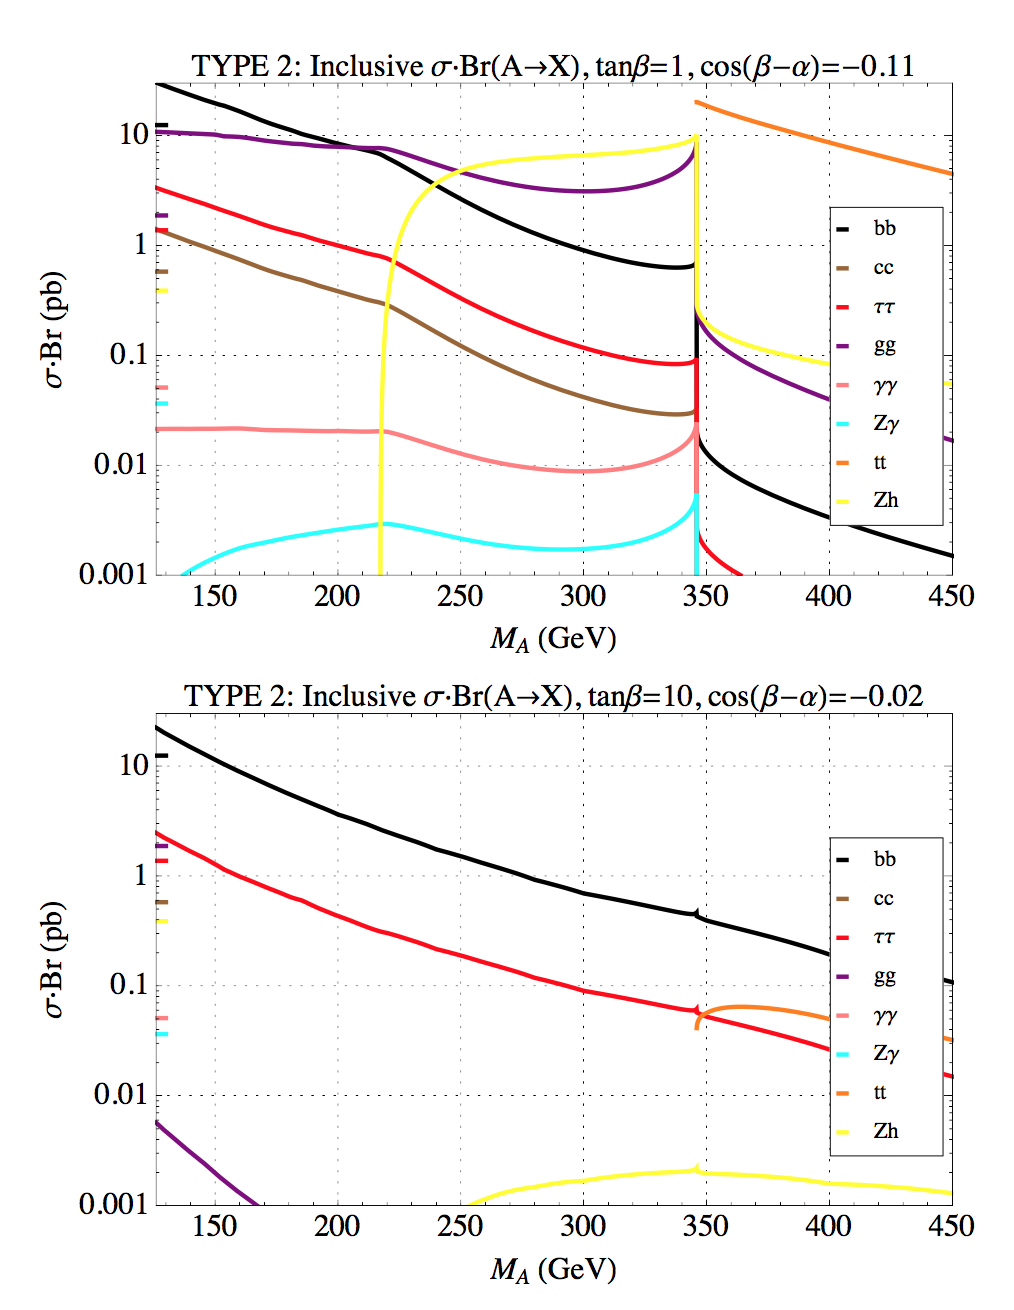
\includegraphics[width=0.484\textwidth]{./Theory/Figures/typeII2HDMxsbrA.png}}
\end{center}
\caption[Inclusive production \xsbr for an example of a type-II 2HDM, for the \PHiggs and \PHiggsps boson.]{Inclusive production \xsbr for an example
of a type-II \ac{2HDM}, for (a) the \PHiggs boson and (b) the \PHiggsps boson. The
top figures use \tanb=1 and $\cos{(\beta-\alpha)}=-0.11$, the bottom
figures are made for \tanb=10 and $\cos{(\beta-\alpha)}=-0.02$. At low \tanb~the \Htohh and
\AtoZh decays are enhanced for masses up to $350\,\GeV$ \cite{2HDM-II}.}
\label{fig:2hdm_Hxsbr}
\end{figure}


\section{MSSM benchmark scenarios}
\label{sec:theory_BSM_models}
Because the MSSM contains a large number of
SUSY-breaking parameters that affect the Higgs
sector, it is usual to define benchmark scenarios 
in which the only free parameters are \mA~and \tanb.
In these scenarios the SUSY parameters entering in 
the radiative corrections are fixed.

The parameters that need to be fixed in the benchmark scenarios are the 
\ac{SUSY} breaking scale $M_{\text{SUSY}}$, which is also the mass scale of the third generation squarks;
the higgsino mass parameter $\mu_{\text{MSSM}}$; the U(1) and SU(2) gaugino mass parameters, $M_1$ and $M_2$;
the masses of the stau, $m_{\tilde{\ell}_3}$, and the gluino, $m_{\tilde{g}}$; the 
trilinear couplings of the stops, sbottoms and staus to the Higgs field ($A_{\Ptop}$, $A_{\Pbottom}$ and $A_{\Pgt}$); and the 
stop, sbottom and stau mixing parameters ($X_{\Ptop}$, $X_{\Pbottom}$ and $X_{\tau}$).

Some of these parameters can be related to each other. For example,
$X_{\Ptop}$, $X_{\Pbottom}$ and $X_{\Pgt}$ can be expressed as:
\begin{equation}\label{eqn:trilinear_couplings}
\begin{split}
&X_{\Ptop} = A_{\Ptop}-\mu_{\text{MSSM}}\cot{\beta},\\
&X_{\Pbottom} = A_{\Pbottom}-\mu_{\text{MSSM}}\tan{\beta},\\
&X_{\Pgt} = A_{\Pgt} - \mu_{\text{MSSM}}\tan{\beta}.
\end{split}
\end{equation}
In addition, $M_1$ is fixed via the unification
relation,
\begin{equation}
M_1 = \frac{5}{3}M_2\tan{\theta_W}^2.
\end{equation}
%where $\theta_w$ is defined by $\cos{\theta_w} = \frac{m_W}{m_Z}$.
Some additional parameters which only have a
small effect on the MSSM Higgs boson sector are 
fixed to values compatible with 
exclusion limits from direct searches in all benchmark scenarios. The masses
of the first and second generation squarks are set to $1.5\,\TeV$, 
and the masses of the first and second generation sleptons to $500\,\GeV$. The trilinear
couplings of the first and second generation squarks and sleptons are taken to be zero.
%Since the discovery of the 125 GeV Higgs boson, only the MSSM benchmark
%scenarios 
%which contain a light Higgs boson with a mass of around 125 GeV
%are still accessible.
% in the mmax scenario the benchmark values have been chosen h
%such that the mass of the light CP-even Higgs boson is maximized for fixed tanβ and large
%MA (the scale of the soft SUSY-breaking masses in the stop and sbottom sectors, which
%sets the mass scale for the corresponding supersymmetric particles, has been fixed to 1 TeV
%in this scenario). This scenario is useful to obtain conservative bounds on tanβ for fixed
%values of the top-quark mass 

\subsection{The $m_{\PHiggslight}^{\text{mod+}}$ scenario}
\label{sec:theory_BSM_models_mhmodp}
The $m_{\PHiggslight}^{\text{mod+}}$ scenario \cite{MSSM-benchmark-scenarios}
is a modification of the $m_{\PHiggslight}^{\text{max}}$ scenario \cite{MSSM-mhmax}. The $m_{\PHiggslight}^{\text{max}}$ scenario, which
was used for interpretations of \ac{MSSM}
 Higgs boson searches at LEP and the Tevatron, allows
the mass of the light Higgs boson to reach the highest a-priori expected 
value of around $135\,\GeV$ for high \mA. There is only a small area of the \mA-\tanb~plane
in this scenario where the mass of the light Higgs boson is compatible with the
observed $125\,\GeV$ state. The modifications to the parameters of the $m_{\PHiggslight}^{\text{max}}$ 
scenario address this issue. In the $m_{\PHiggslight}^{\text{mod+}}$ scenario $M_{\text{SUSY}}$ is chosen
to be $1\,\TeV$. The stop mixing parameter is positive, $X_{\Ptop}= 1.5 M_{\text{SUSY}}$.
%This gives better agreement with muon g-2 results while the mhmod- scenario
%negative stop mixing (-1.9 M_SUSY) results in better agreements with B(b->sgamma) 
%meausrements 
The remaining parameters are set as $\mu_{\text{MSSM}}=200\,\GeV$, $m_{\tilde{g}} = 1.5\,\TeV$,
$m_{\tilde{\ell}_3} = 1\,\TeV$, and $A_{\Pbottom}=A_{\Ptop}=A_{\Pgt}$. 
%Figure \ref{fig:mhmodp_mh}a
%shows the mass of the light Higgs boson in the $m_{h}^{\text{mod+}}$ scenario, showing
%that its mass is compatible with 125 GeV over a large part of the parameter space. Masses within 
%a window $\pm 3$ GeV around 125 GeV are considered compatible with 125 GeV, where the 3 GeV
%variation corresponds to the theoretical uncertainty on the \ac{MSSM} prediction for \mh.


Figure \ref{fig:mhmodp_xs} shows the cross sections of
gluon fusion and b-associated production of the \PHiggs boson 
in the $m_{\PHiggslight}^{\text{mod+}}$ scenario. Gluon fusion 
production dominates at low \tanb, while b-associated production has a larger cross section
at high \tanb. The behaviour of the production cross sections of the \PHiggsps boson
is similar.

\begin{figure}[h!]
\begin{center}
\subfloat[$\sigma(\Pg\Pg\rightarrow \PHiggs)$]{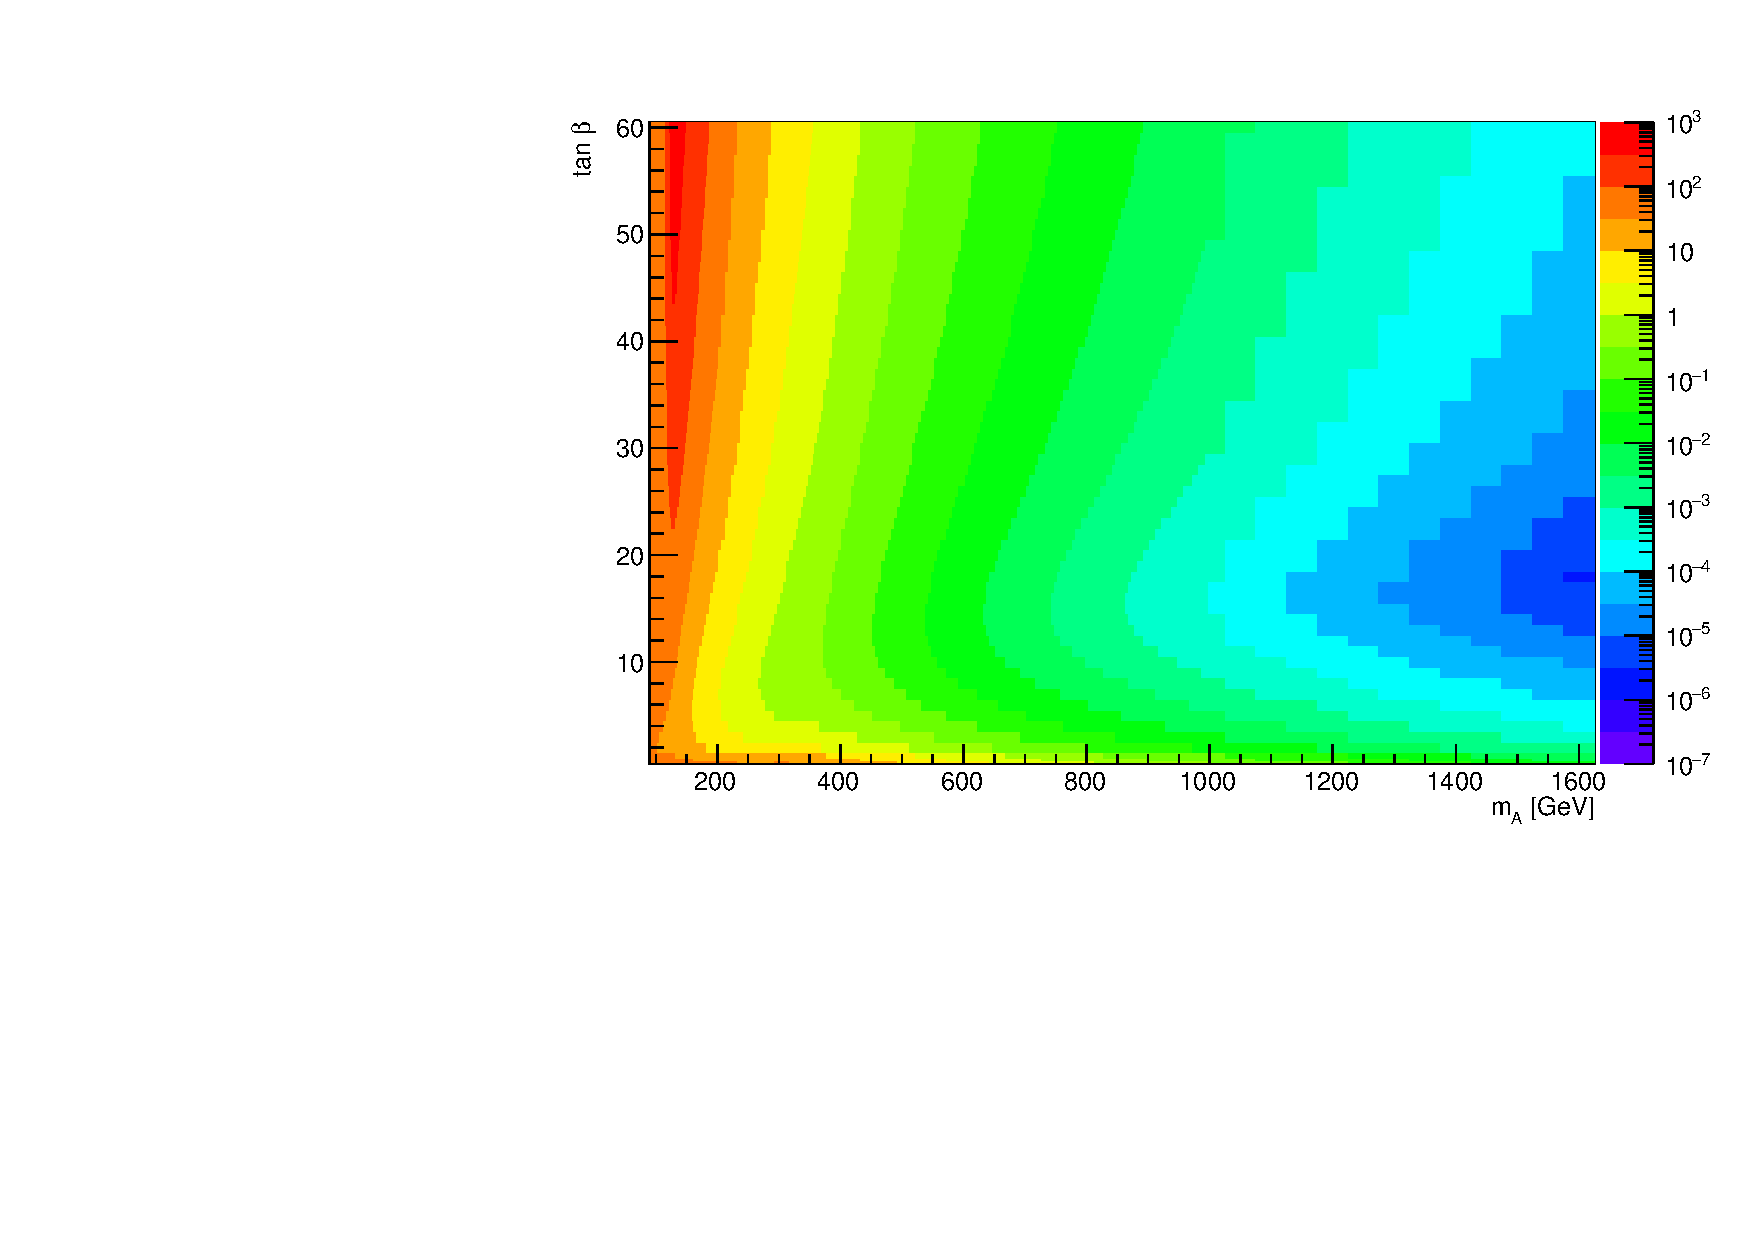
\includegraphics[width=0.5\textwidth]{./Theory/Figures/xs_ggH_mhmodp.pdf}}
\subfloat[$\sigma(\Pg\Pg\rightarrow \Pbottom\Pbottom\PHiggs)$]{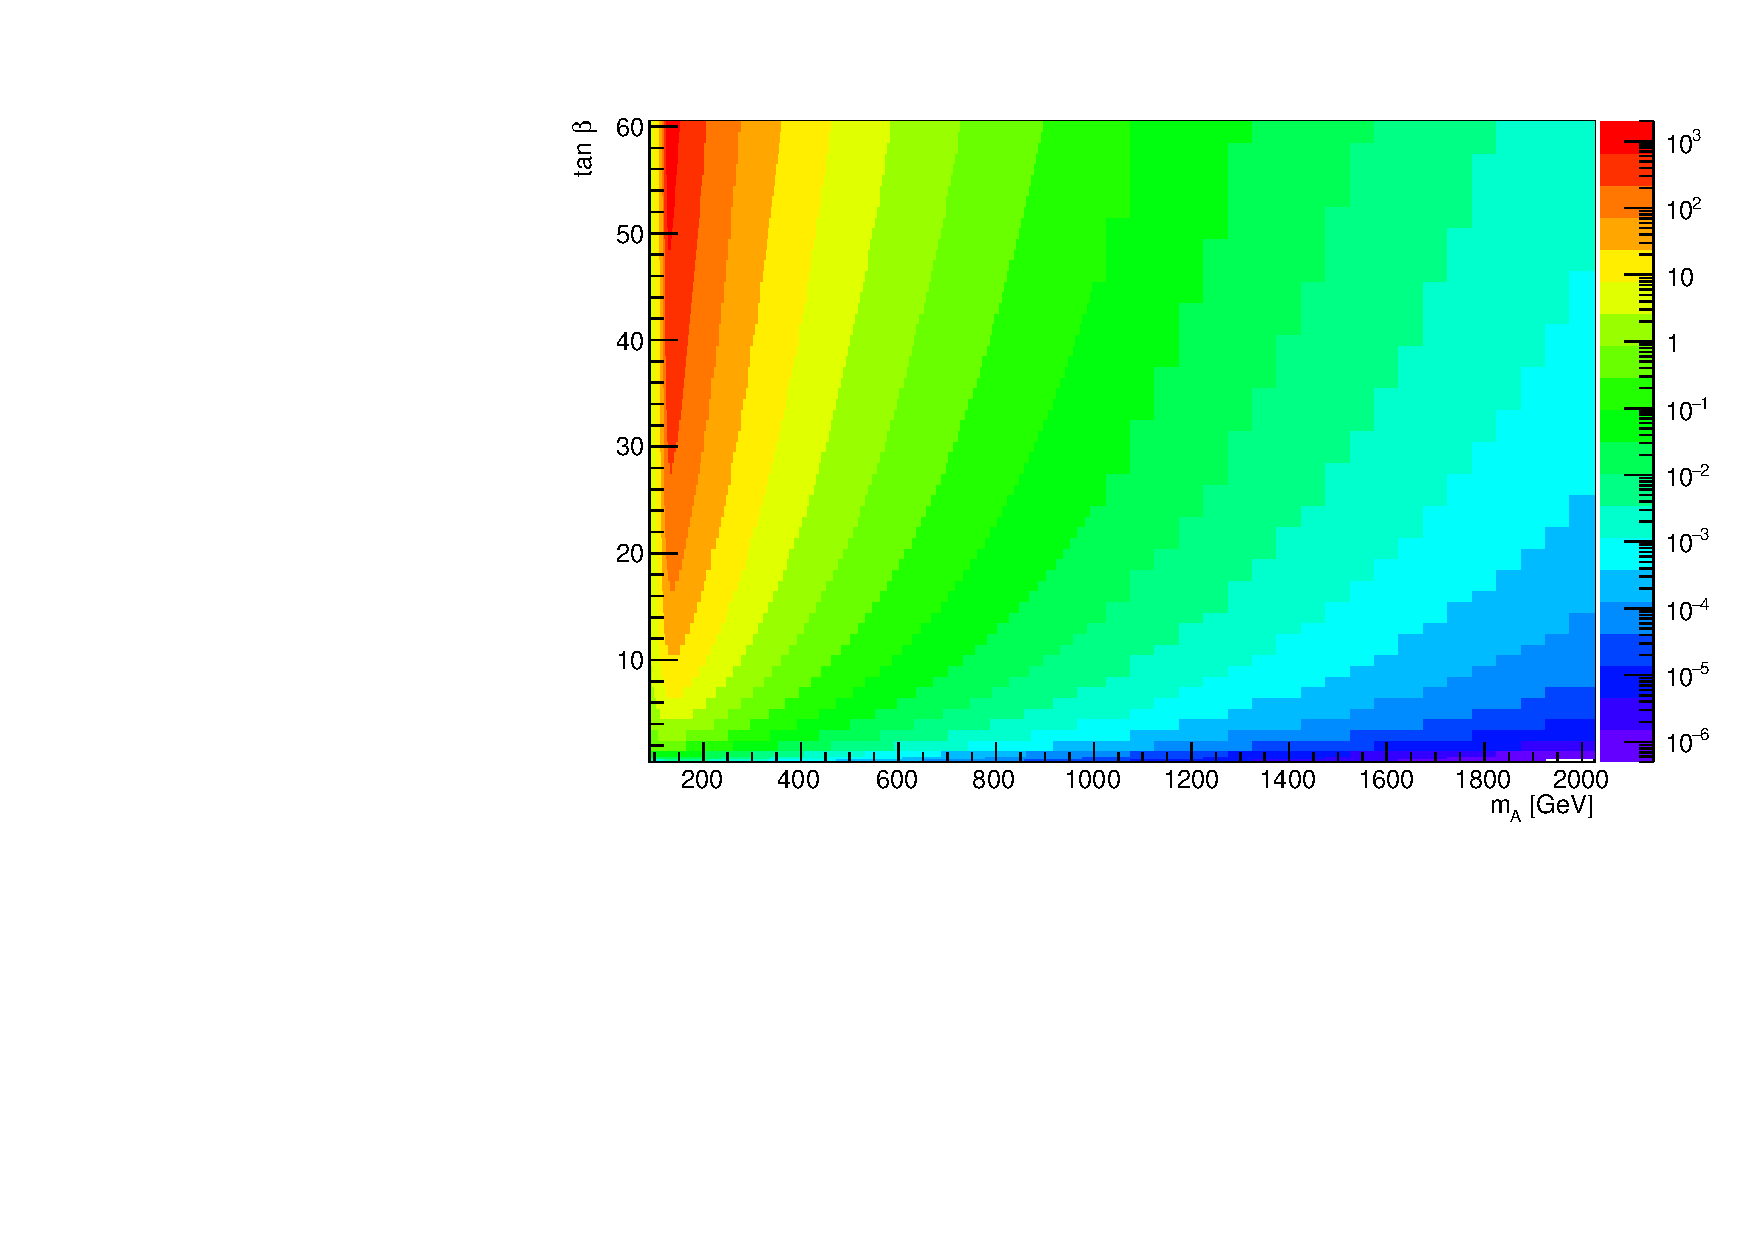
\includegraphics[width=0.5\textwidth]{./Theory/Figures/xsbbH4F_mhmodp.pdf}}
\end{center}
\caption[Production cross sections of  gluon fusion and b-associated
production of the \PHiggs boson in the $m_{\PHiggslight}^{\text{mod+}}$ scenario.]{Production cross section of (a) gluon fusion production and (b) b-associated production of the \PHiggs boson
in the $m_{\PHiggslight}^{\text{mod+}}$ scenario. The gluon fusion production cross section is larger at low \tanb, while
the b-associated production cross section is larger at high \tanb. These values are based on the
calculations in reference \cite{YR3}.}
\label{fig:mhmodp_xs}
\end{figure}

Figure \ref{fig:mhmodp_br} shows the branching ratios of the \PHiggs and \PHiggsps 
bosons into $\tau\tau$. The branching ratios into $\tau\tau$ are enhanced, especially at
high \tanb, showing how this decay channel is useful for MSSM Higgs boson searches.

\begin{figure}[h!]
\begin{center}
\subfloat[$\mathcal{B}(\PHiggs \rightarrow \tau\tau)$]{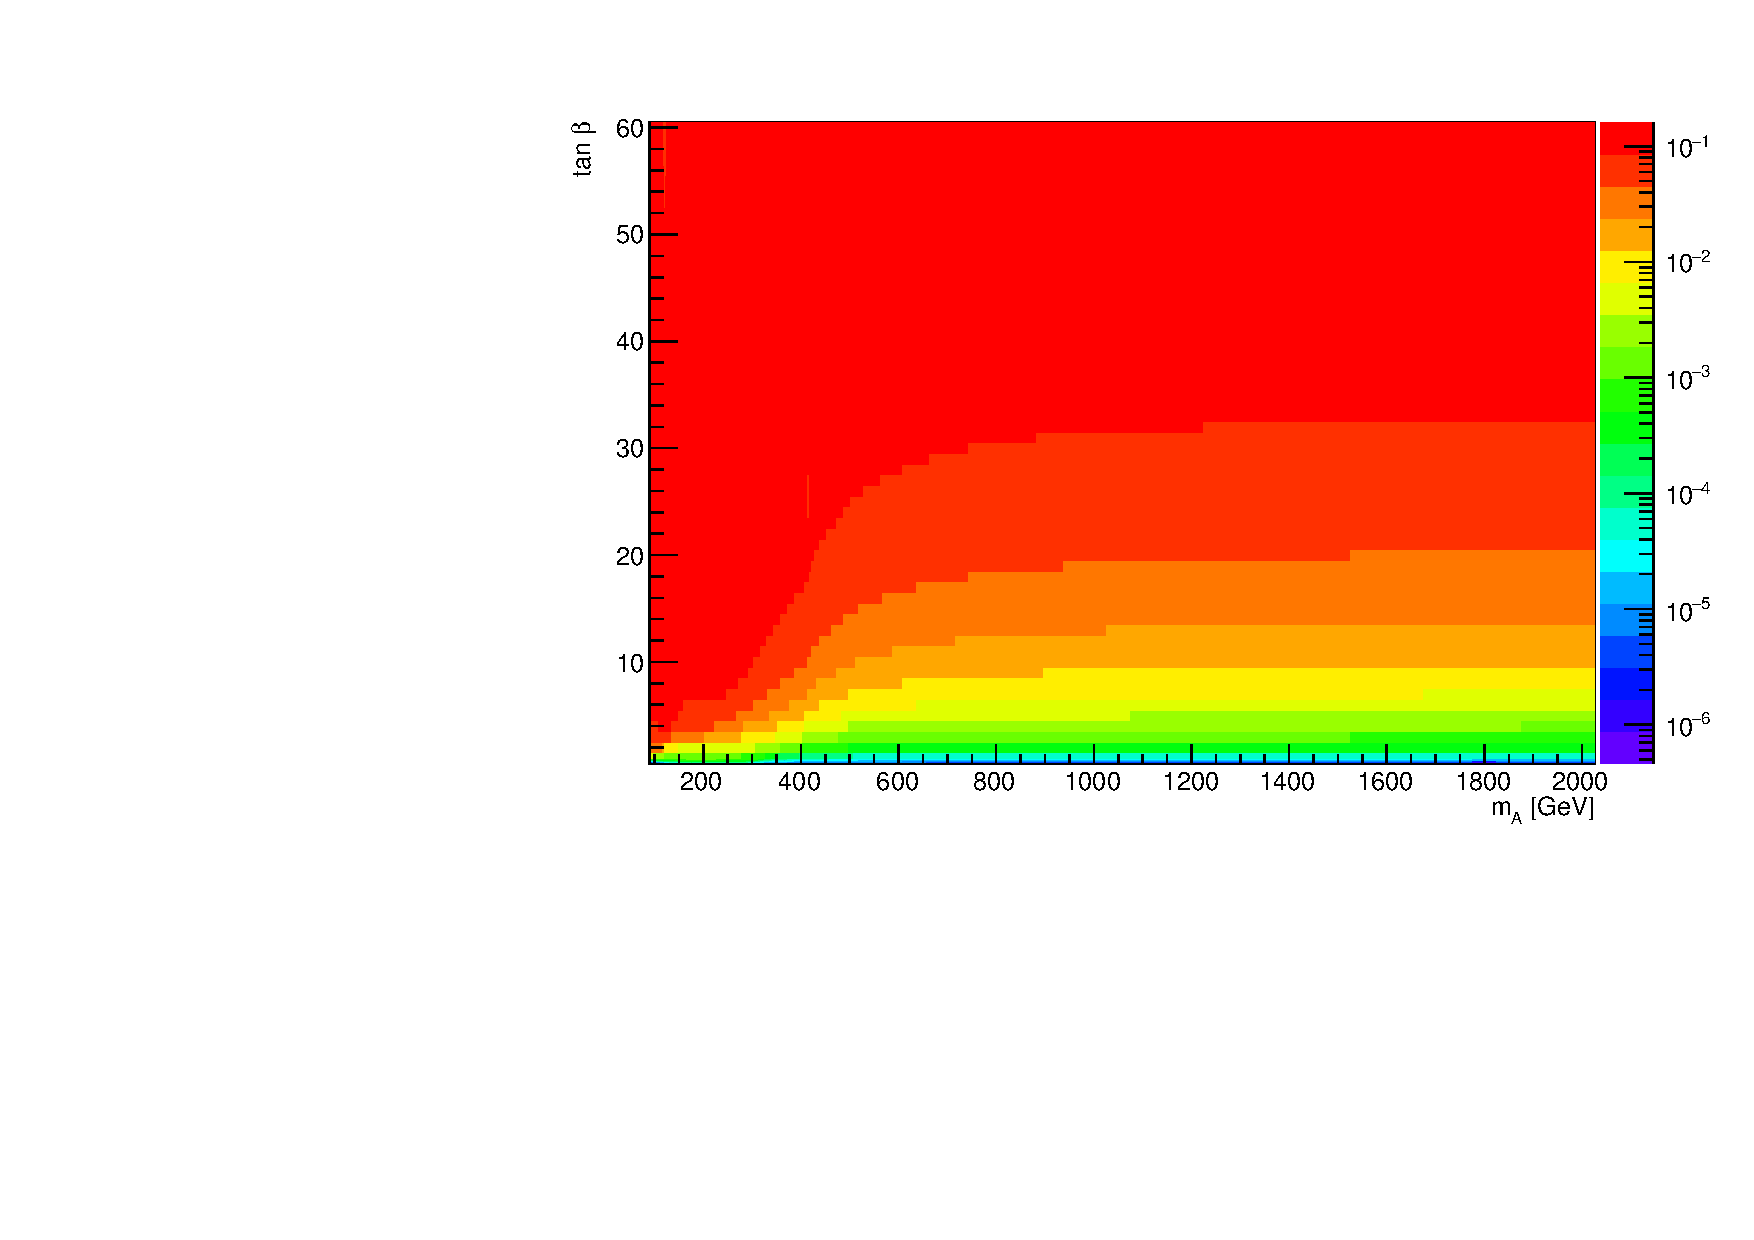
\includegraphics[width=0.5\textwidth]{./Theory/Figures/brHtautau_mhmodp.pdf}}
\subfloat[$\mathcal{B}(\PHiggsps \rightarrow \tau\tau)$]{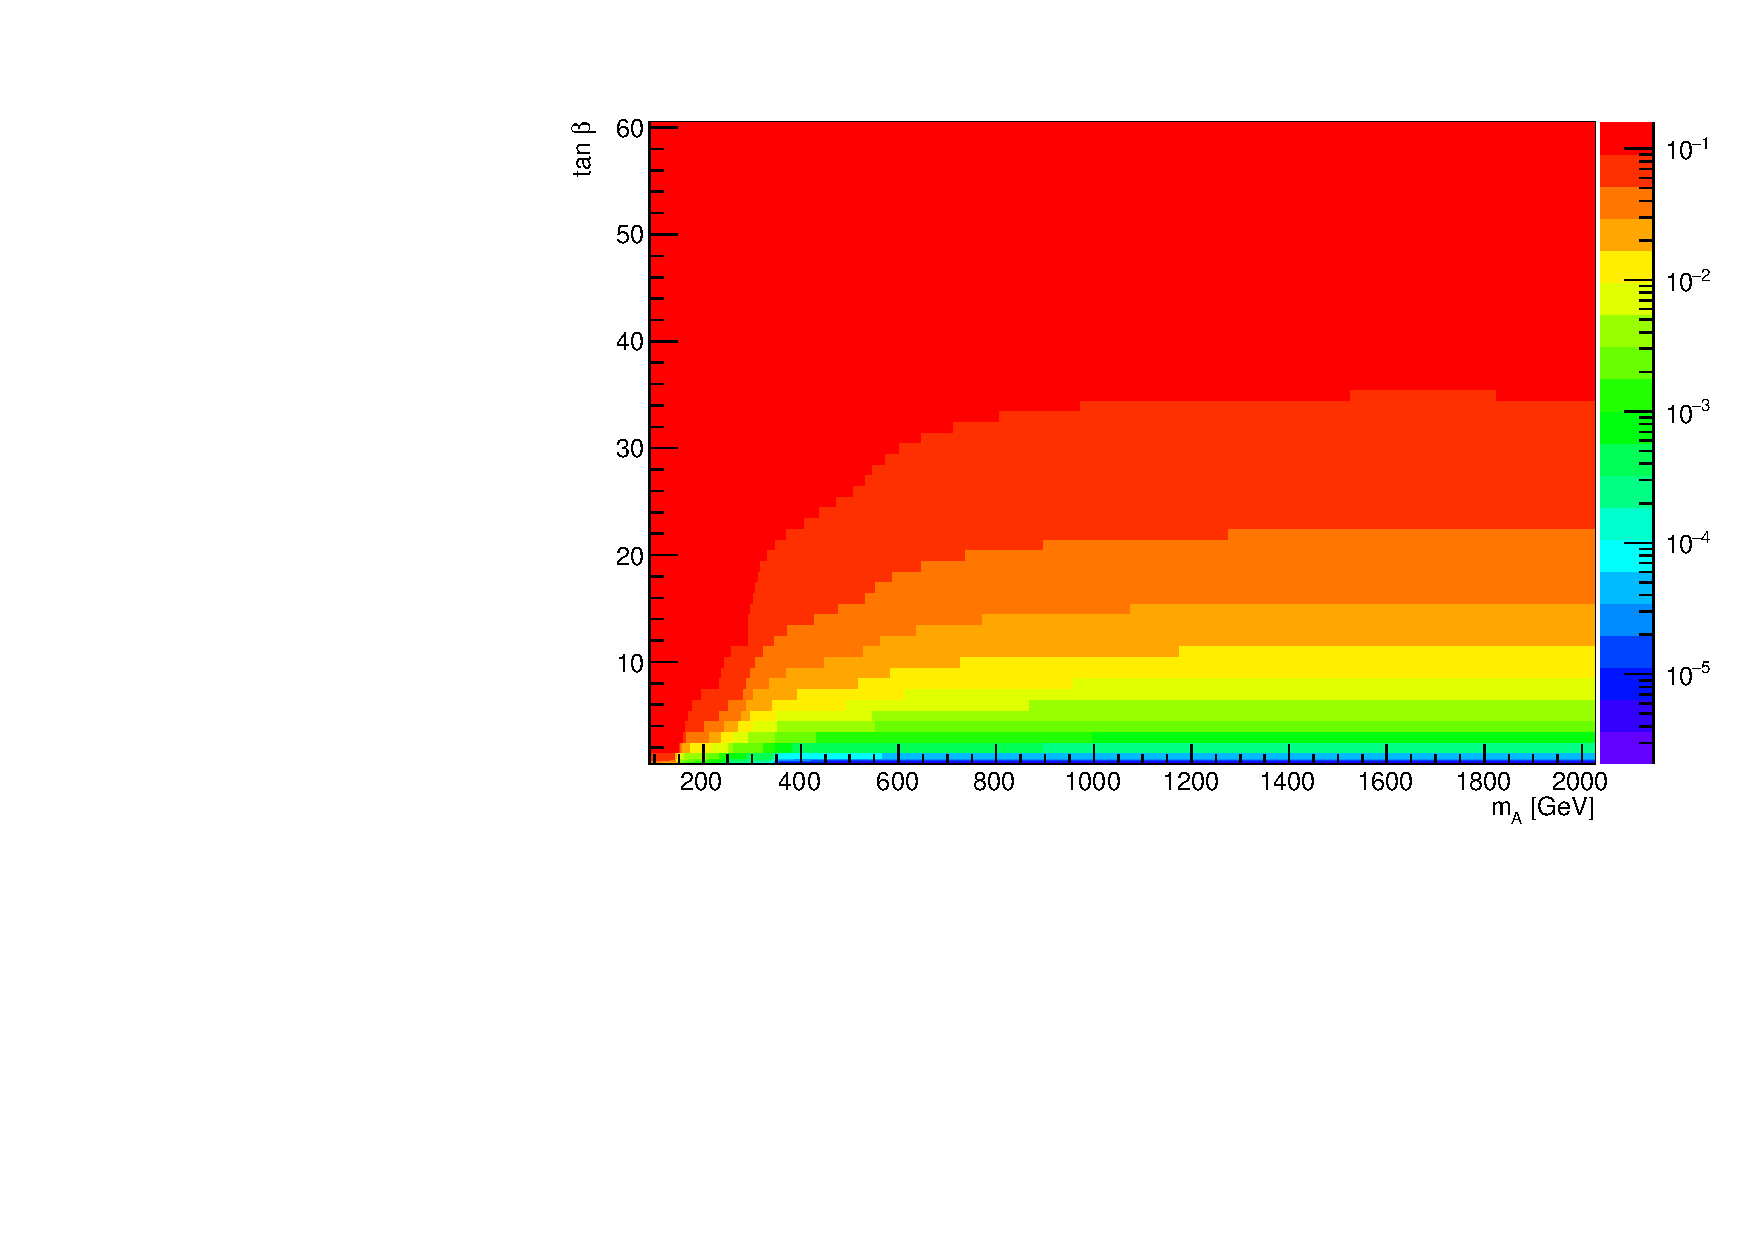
\includegraphics[width=0.5\textwidth]{./Theory/Figures/brAtautau_mhmodp.pdf}}
\end{center}
\caption[Branching ratios of the \PHiggs and \PHiggsps bosons into $\tau\tau$.]{Branching ratios of (a) the \PHiggs boson and (b) the \PHiggsps boson into $\tau\tau$. The branching
ratios into $\tau\tau$ are enhanced at high \tanb. These values are based on the
calculations in reference \cite{YR3}.}
\label{fig:mhmodp_br}
\end{figure}


\subsection{MSSM scenarios at low \tanb}
\label{sec:mssm_theory_lowtb}
The mass of the light Higgs boson in the \ac{MSSM} is said to
be compatible with $125\,\GeV$ if the light Higgs boson mass lies within 
$\pm 3\,\GeV$ of $125\,\GeV$. This mass window
corresponds to the theoretical uncertainty on the \ac{MSSM} prediction for \mh.
A large area of the \mbox{\mA-\tanb}~plane in the $m_{\PHiggslight}^{\text{mod+}}$ 
scenario contains a light Higgs boson with a mass compatible with
$125\,\GeV$. However, at low values of \tanb~this is not the case.
This is illustrated in figure \ref{fig:mhmodp_mh}a, where the mass of the light Higgs
boson in the $m_{\PHiggslight}^{\text{mod}+}$ scenario is shown.
The low \tanb~regime can be re-opened
if $M_{\text{SUSY}}$ is allowed to be greater than $3\,\TeV$ \cite{MSSM-reopen}. 
%But not too large, see ref above!
%Figure \ref{fig:tanb_accessibility} shows contours of constant
%light Higgs boson mass as a function of \tanb~and $M_{\text{SUSY}}$.
%It indicates that values of \mh~can be compatible with 125$\pm$3 GeV
%for \tanb~values down to 1 if $M_{\text{SUSY}}$ is around 100-1000 TeV. 
%\tanb~values of 3-5 are even accessible for $M_{\text{SUSY}}$ of around 10 TeV.
%
%\begin{figure}[h!]
%\begin{center}
%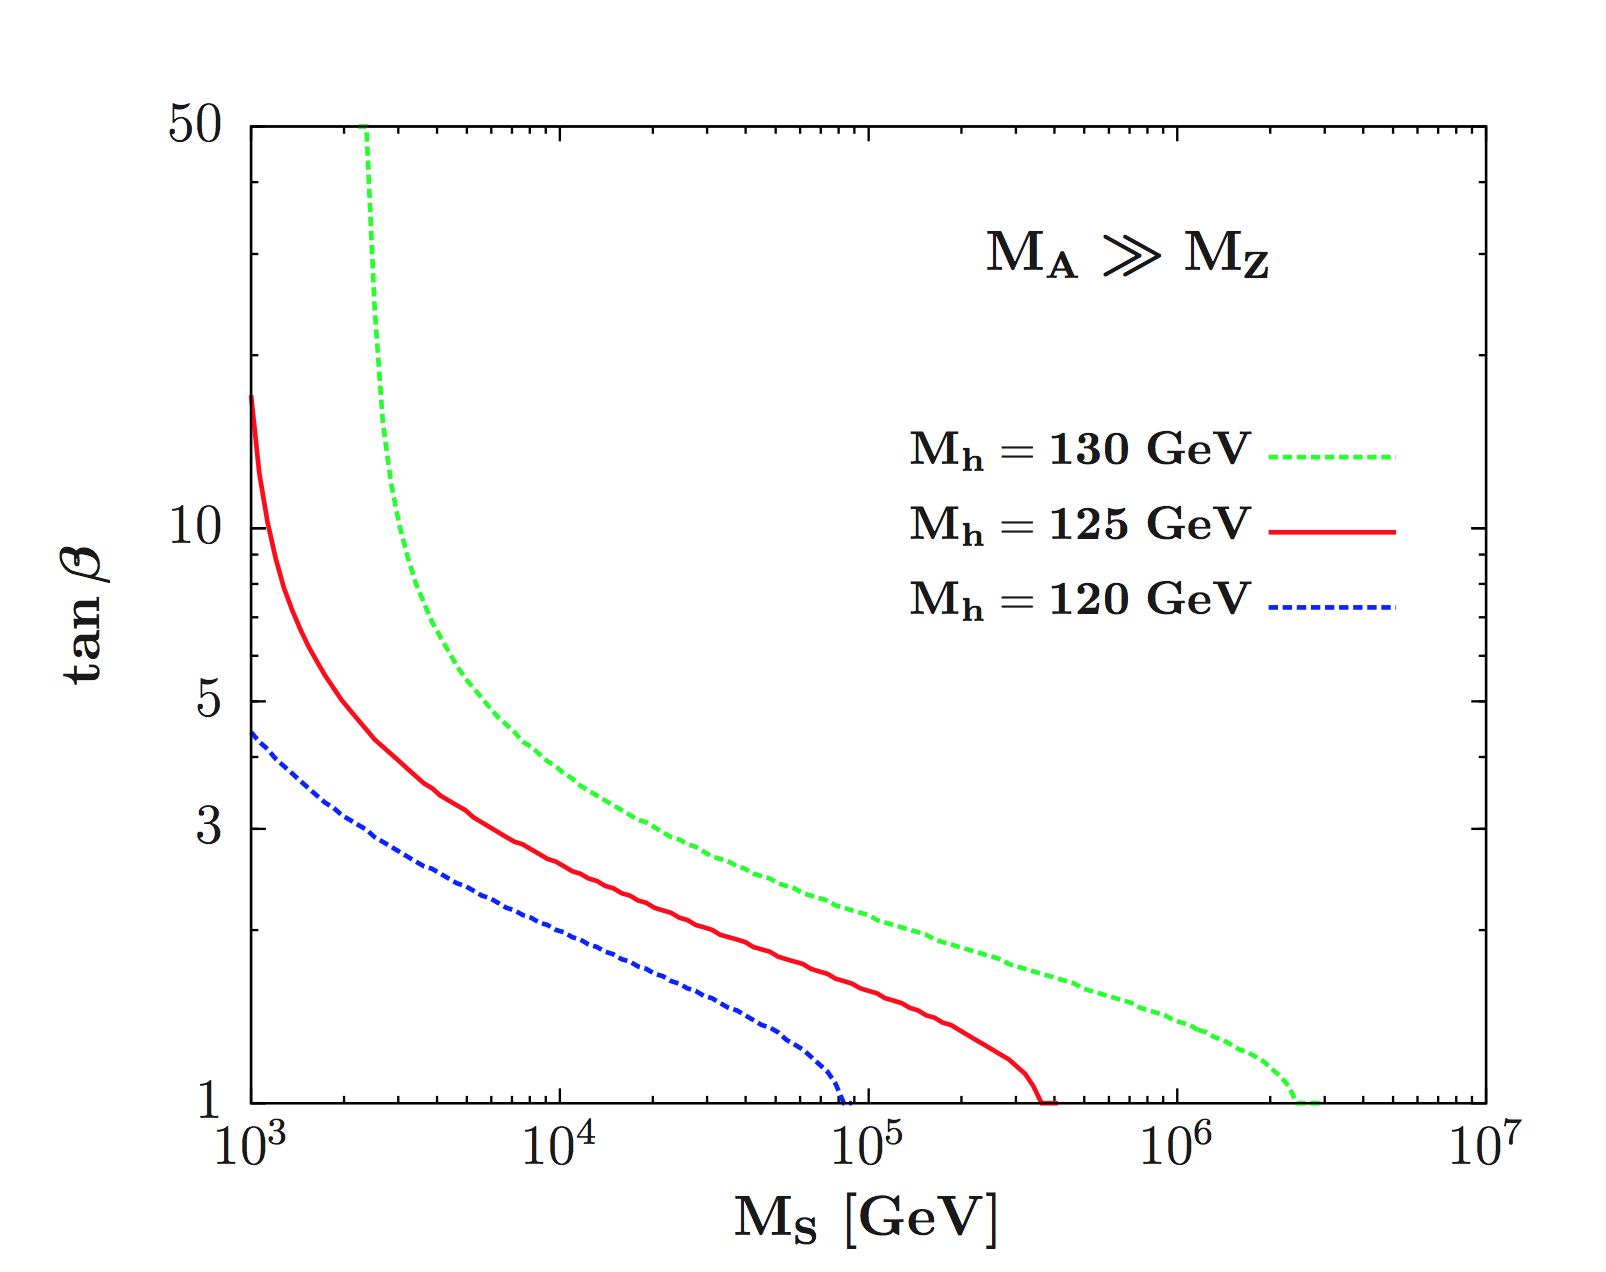
\includegraphics[width=0.5\textwidth]{./Theory/Figures/tanb_accessibility.png}
%\end{center}
%\caption{Contours of constant light Higgs boson mass as a function of \tanb~and $M_{\text{SUSY}}$.
%High values of $M_{\text{SUSY}}$ allow for light Higgs boson masses compatible with
%125 GeV down to low values of \tanb~\cite{hMSSM-2}.}
%\label{fig:tanb_accessibility}
%\end{figure}
%where the ±3 GeV variation corresponds to a rough estimate of the theoretical uncertainty of the MSSM prediction for mh, due to the unknown effect of higher-order correction

Two approches for the definition of an \ac{MSSM} scenario that gives
access to the low \tanb~region have been developed, they will be
discussed in the next sections.

\begin{figure}[h!]
\begin{center}
\subfloat[$m_{\PHiggslight}^{\text{mod}+}$ scenario]{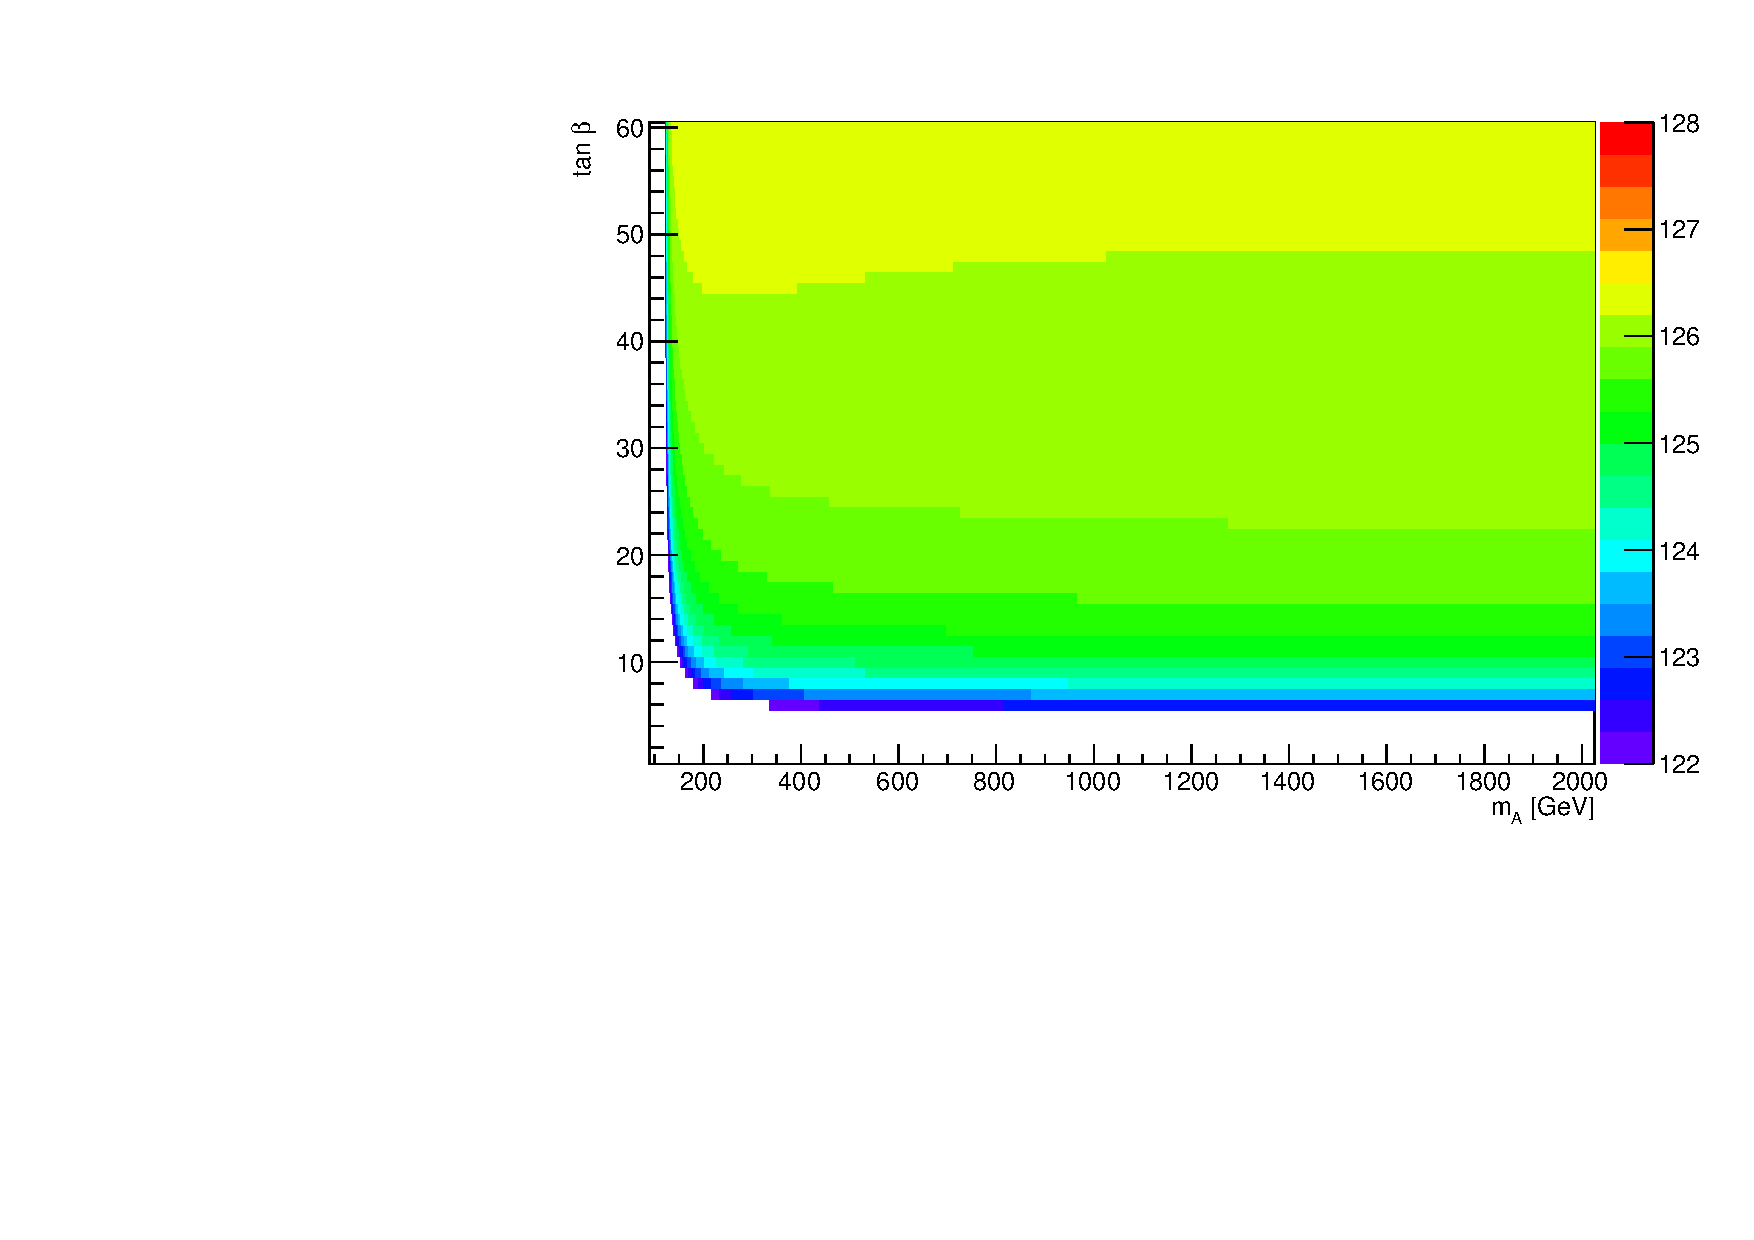
\includegraphics[width=0.5\textwidth]{./Theory/Figures/mh_mhmodp.pdf}}
\subfloat[Low-\tanb~scenario]{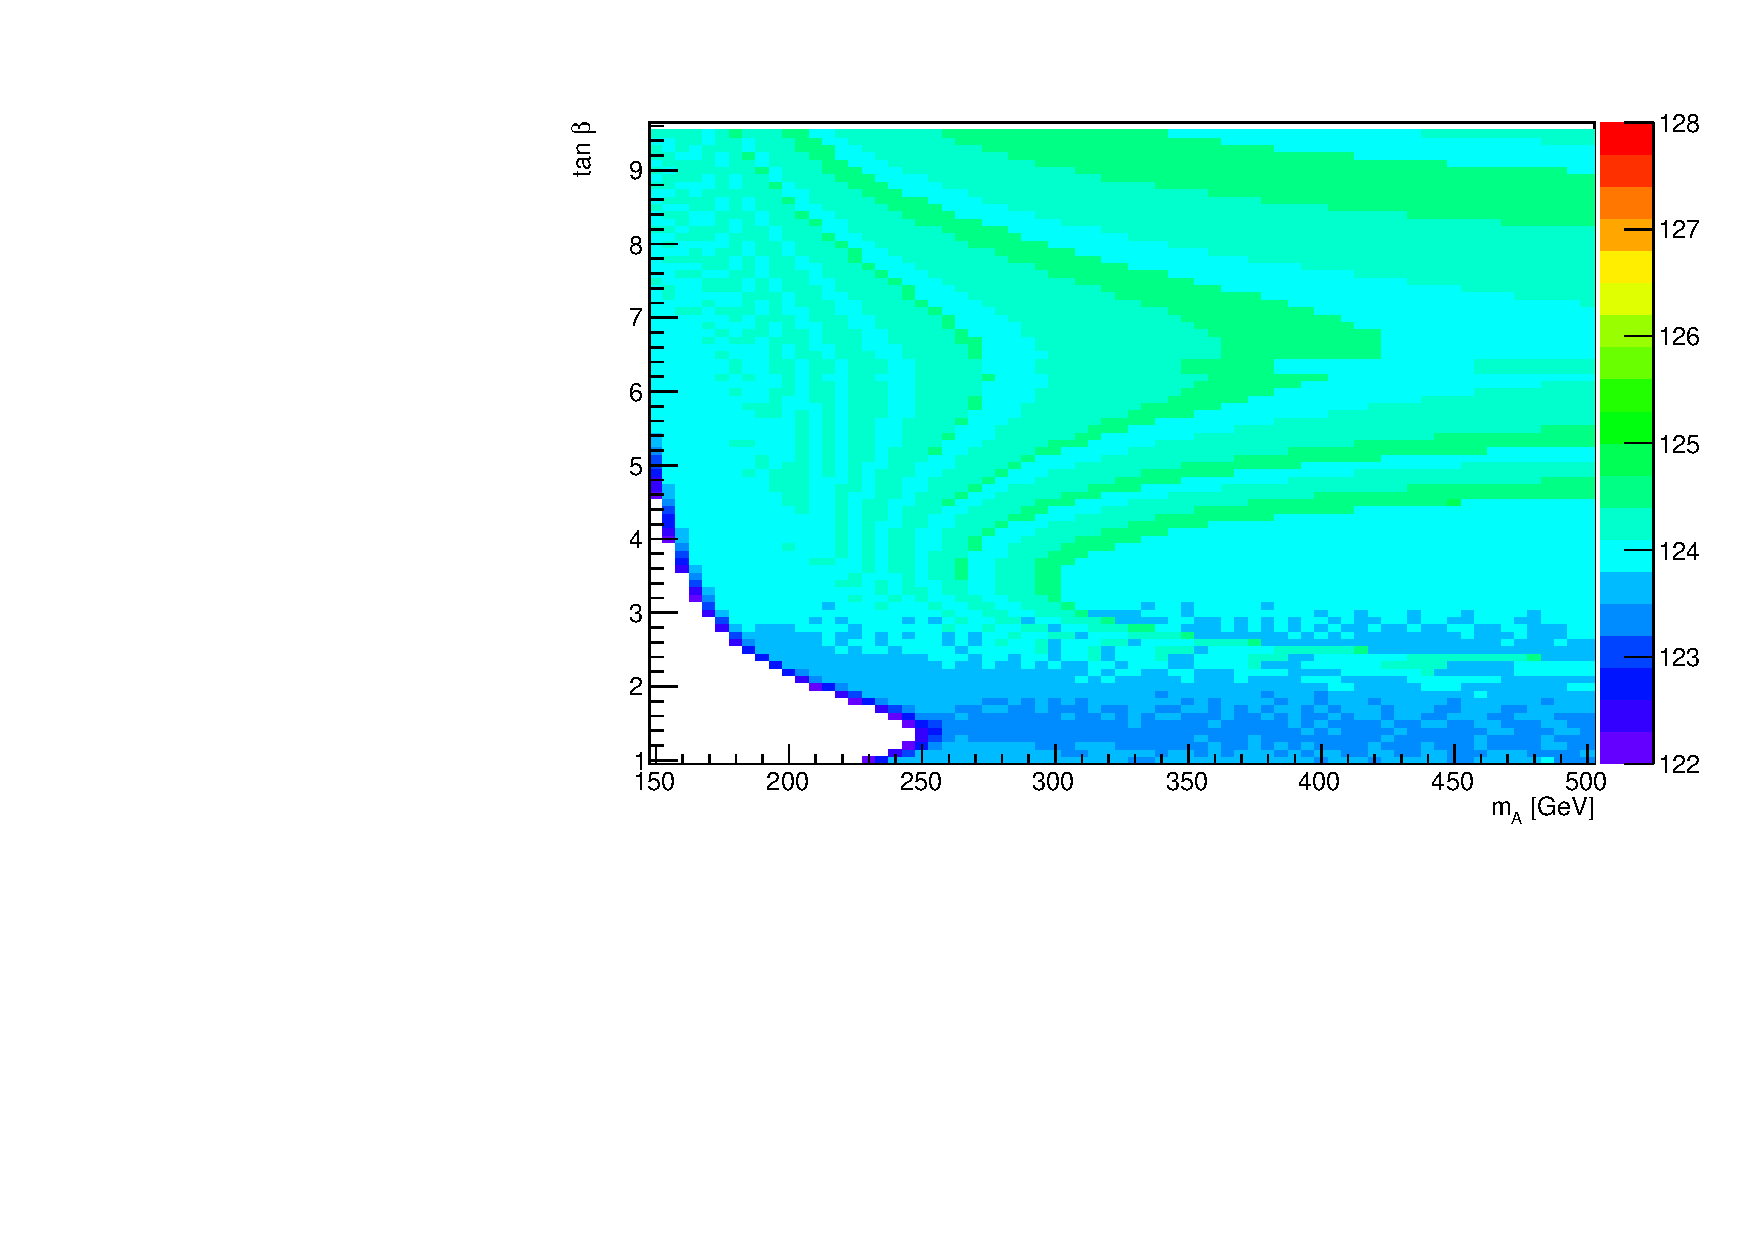
\includegraphics[width=0.5\textwidth]{./Theory/Figures/mh_lowtbhigh.pdf}}
\end{center}
\caption[The mass of the light Higgs boson, \mh, as a function of \mA~and
\tanb~in the $m_{\PHiggslight}^{\text{mod+}}$ scenario and the low-\tanb~scenario.]{The mass of the light Higgs boson, \mh, as a function 
of \mA~and \tanb~in (a) the $m_{\PHiggslight}^{\text{mod+}}$ scenario and (b) the low-\tanb~scenario. The white areas
indicate masses lower than $122\,\GeV$. The figures show that
the mass of the light Higgs boson is compatible with $125\,\GeV$ over a large
part of the \mA-\tanb~plane in the $m_{\PHiggslight}^{\text{mod+}}$ scenario, except at low \tanb. In the low-\tanb~scenario
the mass of the light Higgs boson is compatible with $125\,\GeV$ nearly everywhere. These values are based on the calculations in reference \cite{YR3}.}
\label{fig:mhmodp_mh}
\end{figure}

\subsubsection{The low-\tanb~scenario}
\label{sec:theory_BSM_model_lowtb}
In the low-\tanb~scenario \cite{Hein-low-tb-high,MSSM-lowtanb}, the SUSY parameters entering
the radiative corrections are tuned to obtain a light 
Higgs boson mass of around $125\,\GeV$ in most of the \mbox{\mA-\tanb}~plane considered.
Figure \ref{fig:mhmodp_mh}b shows that, apart from in a corner of \tanb~$=1$--$4$ and 
\mA~$=150$--$250\,\GeV$, \mh~is compatible with $125\,\GeV$.

%\begin{figure}[h!]
%\begin{center}
%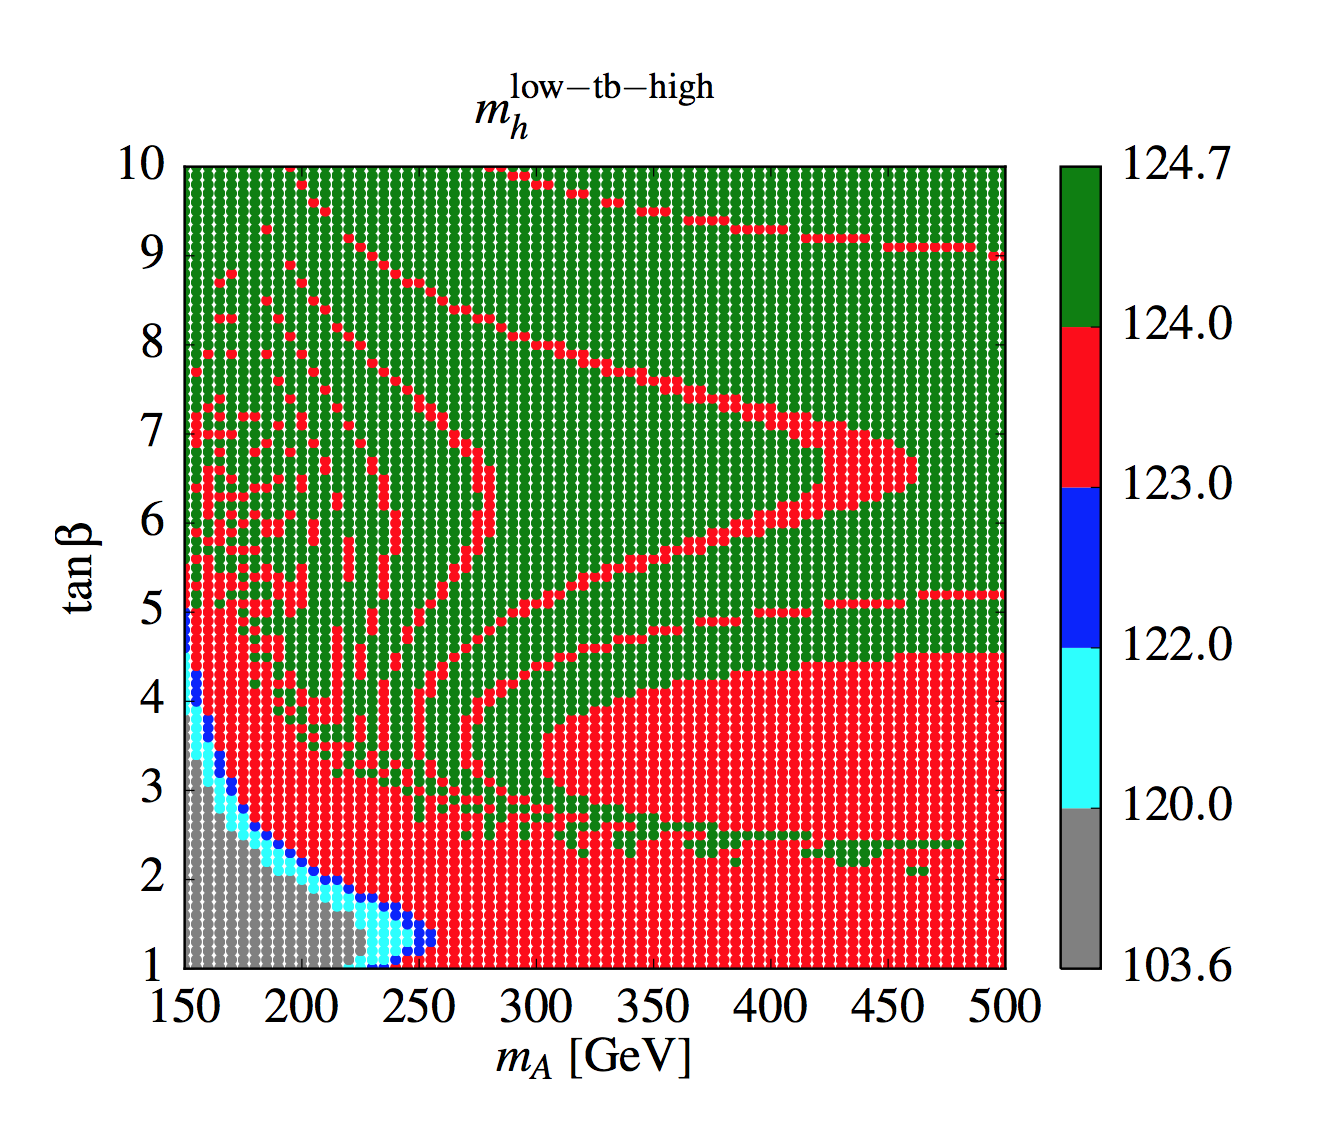
\includegraphics[width=0.5\textwidth]{./Theory/Figures/mh_lowtbhigh.png}
%\end{center}
%\caption{Mass of the light Higgs boson in the \mA-\tanb~plane of the low-\tanb~scenario.
%The mass is compatible with $125\,\GeV$ nearly everywhere \cite{MSSM-lowtanb}.}
%\label{fig:lowtbhigh_mh}
%\end{figure}
To obtain \mh~$\approx125\,\GeV$ over a large part of the parameter
space, 
$M_{\text{SUSY}}$ is not fixed but varies between a few $\TeV$ and $100\,\TeV$, while
varying the parameter $X_{\Ptop}$ as:
\begin{equation}
\begin{split}
\tan{\beta} \leq 2 &: \frac{X_{\Ptop}}{M_{\text{SUSY}}} = 2,\\
2 < \tan{\beta} \leq 8.6 &: \frac{X_{\Ptop}}{M_{\text{SUSY}}} = 0.0375\text{tan}^2\beta - 0.7\tan{\beta} + 3.25,\\
8.6 < \tan{\beta} &: \frac{X_{\Ptop}}{M_{\text{SUSY}}} = 0.
\end{split}
\end{equation}
The other trilinear couplings are set to $2\,\TeV$, with $\mu_{\text{MSSM}}$ set to $1.5\,\TeV$ and $M_2$ to $2\,\TeV$.

The branching ratios of \Htohh and \AtoZh in the low-\tanb~scenario are shown in
figure \ref{fig:lowtbhigh_br}. For both decay channels there are areas in the \mA-\tanb~plane
where the branching ratio is enhanced, indicating how analyses targeting such processes 
can be sensitive in this scenario. %REPHRASE
%The analysis presented in chapter \ref{chap:hhh} is interpreted
%in the low-\tanb~scenario.

\begin{figure}[h!]
\begin{center}
\subfloat[\Htohh]{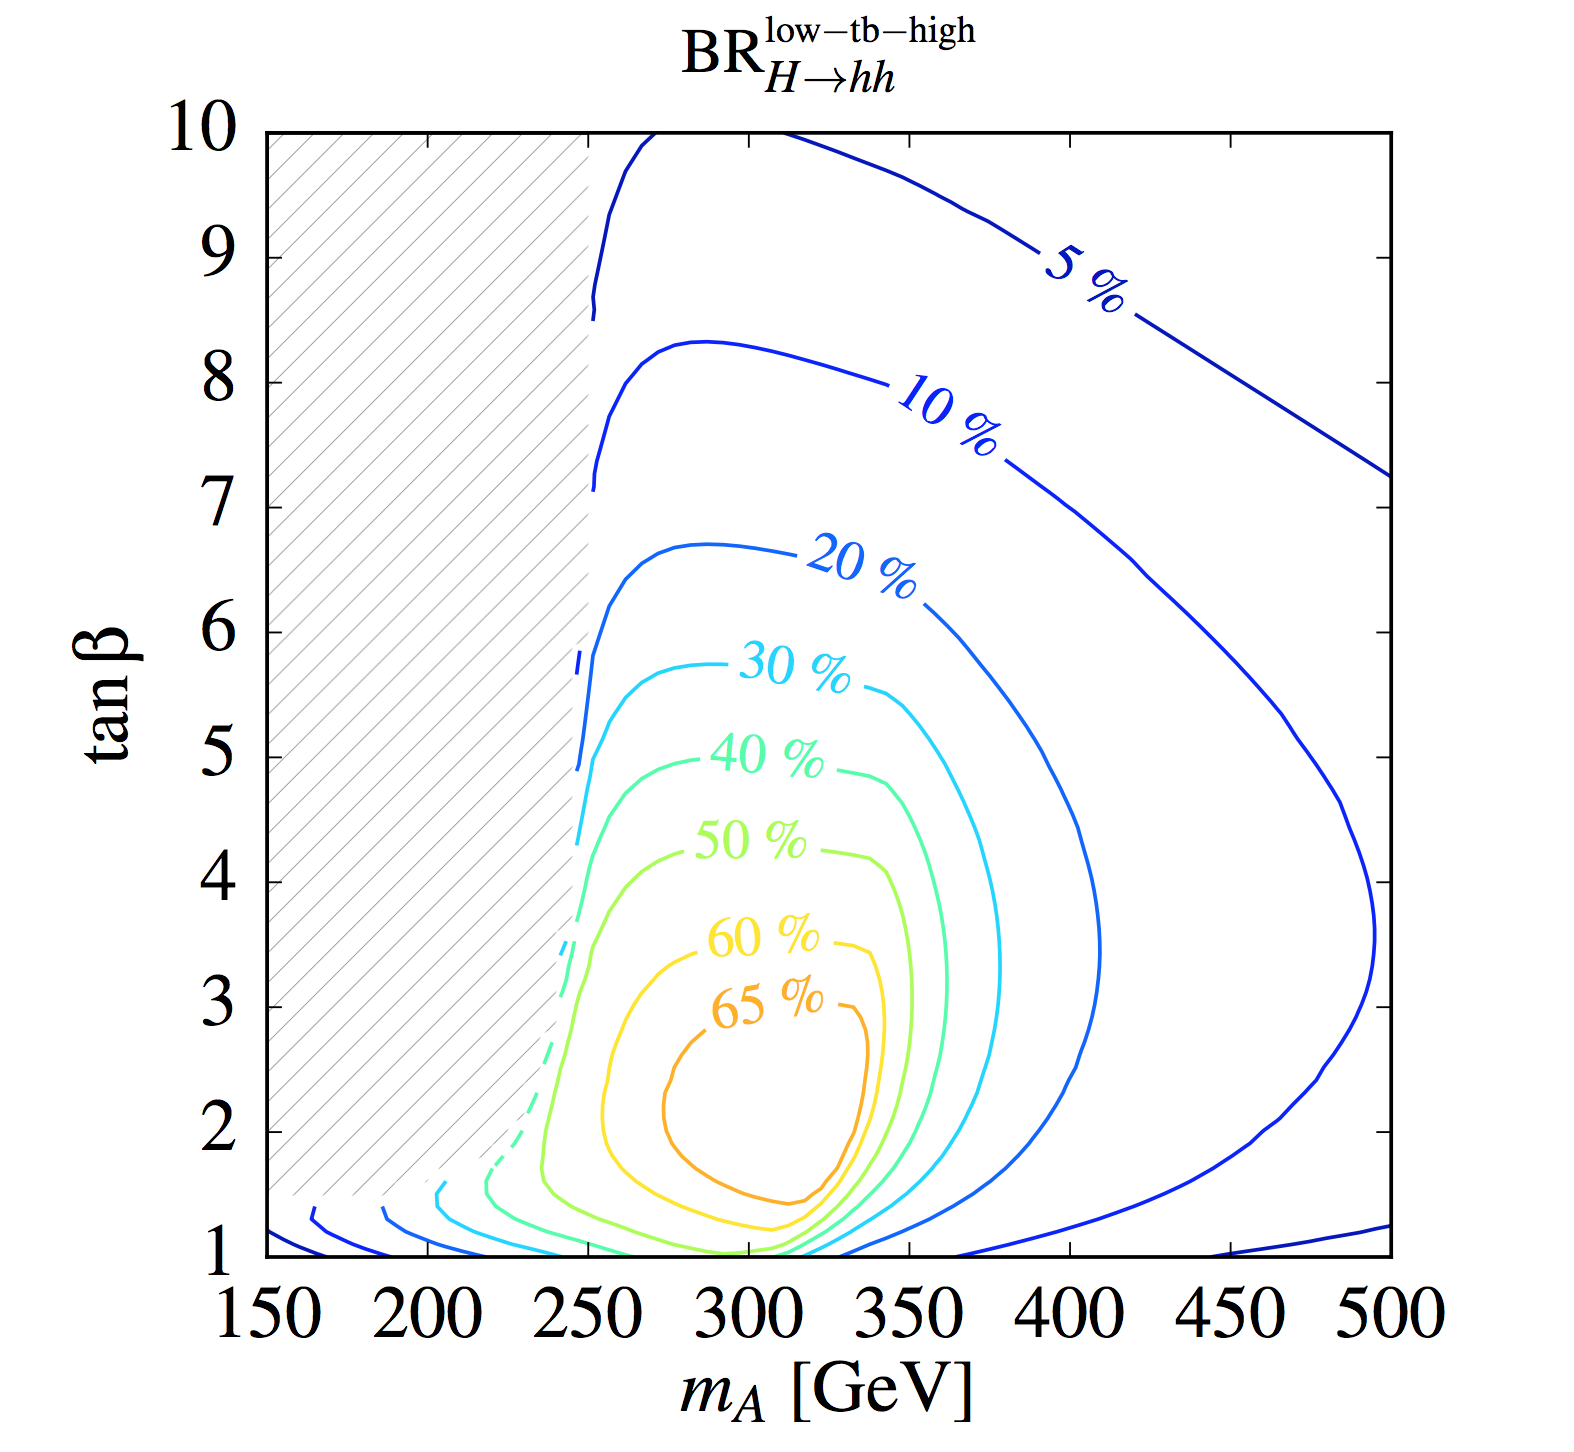
\includegraphics[width=0.5\textwidth]{./Theory/Figures/lowtbhigh_hhbr.png}}
\subfloat[\AtoZh]{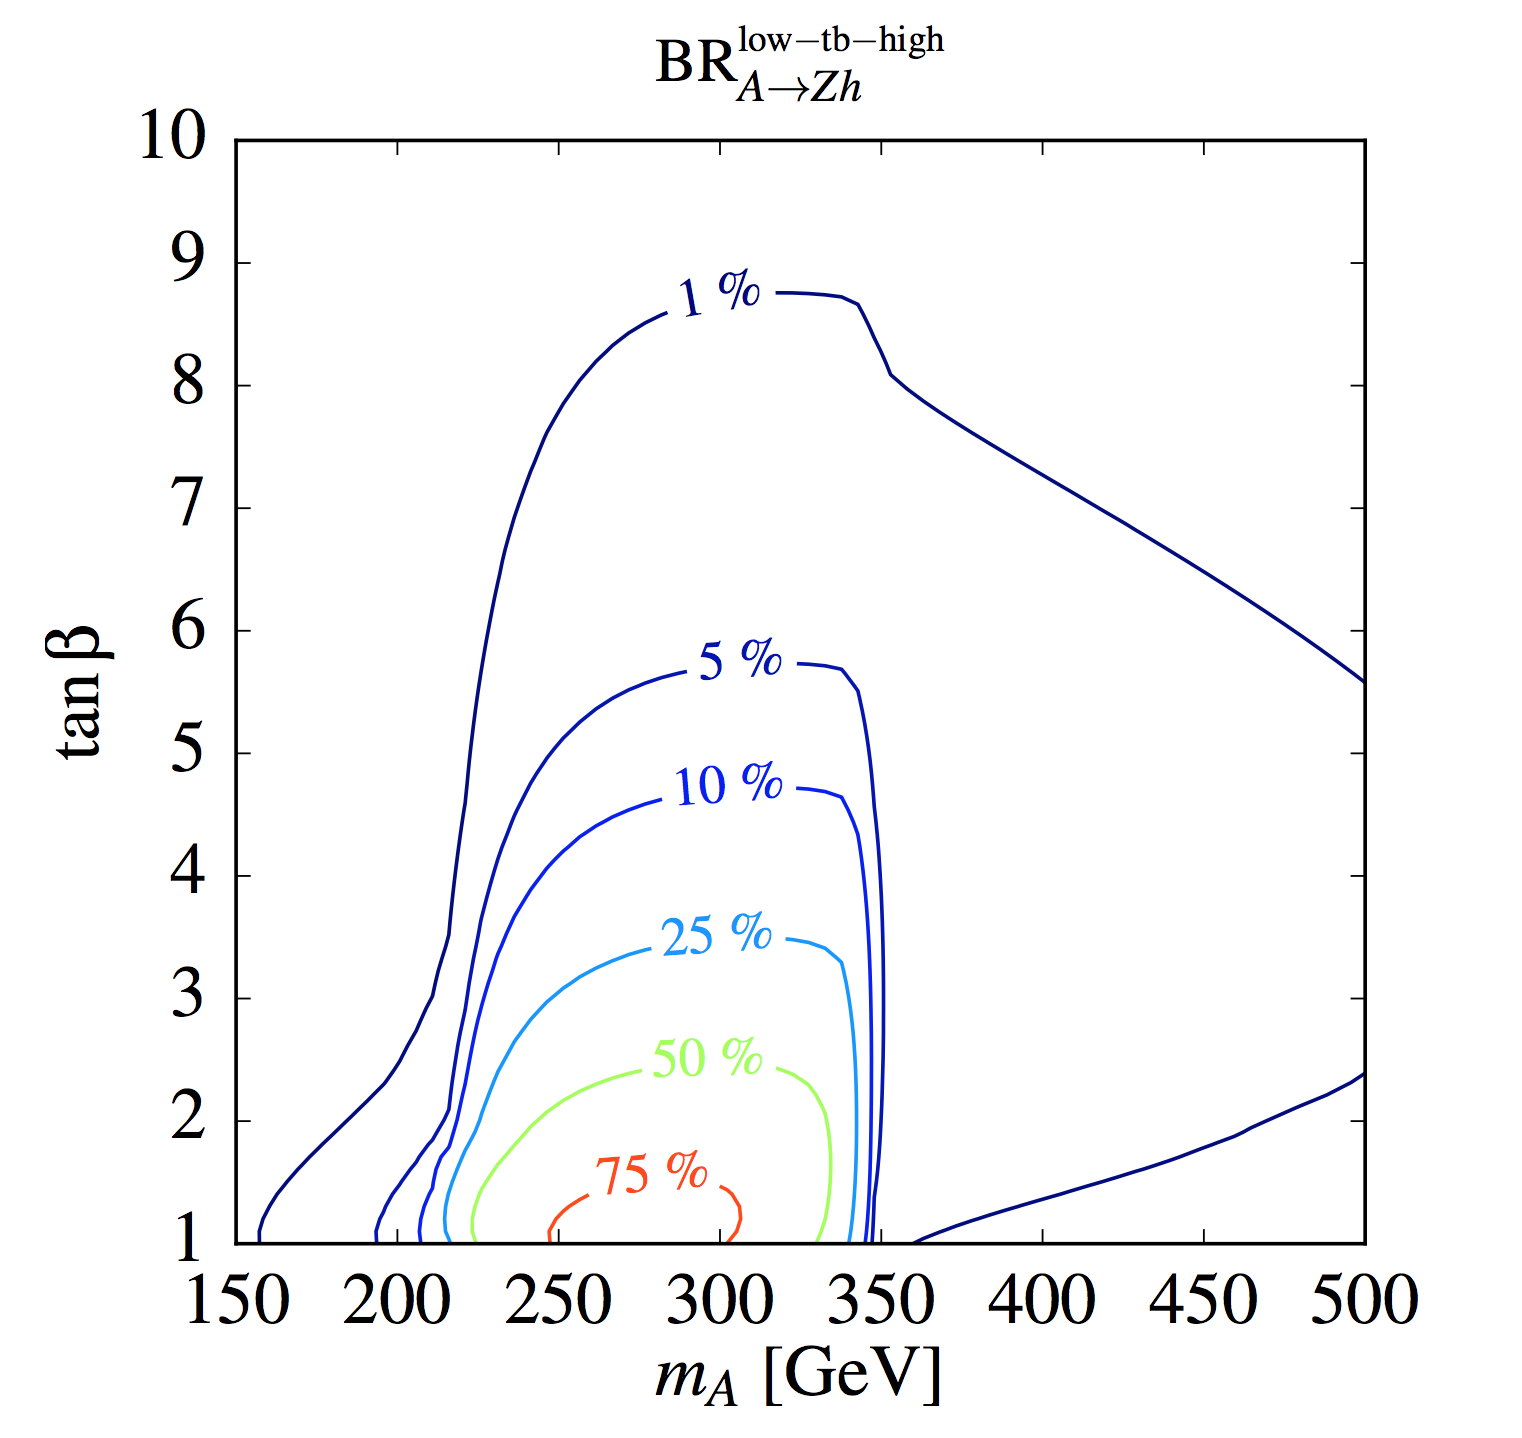
\includegraphics[width=0.5\textwidth]{./Theory/Figures/lowtbhigh_azhbr.png}}
\end{center}
\caption[Branching ratios of \Htohh and \AtoZh in the low-\tanb~scenario.]{Branching ratios of (a) \Htohh and (b) \AtoZh in the low-\tanb~scenario, indicating 
areas where both are significantly enhanced \cite{MSSM-lowtanb}.}
\label{fig:lowtbhigh_br}
\end{figure}

\subsubsection{The hMSSM scenario}
\label{sec:theory_BSM_models_hMSSM}
The hMSSM scenario \cite{hMSSM-1,hMSSM-2} uses a different approach, in
which \mh~$=125\,\GeV$ by construction. 

One of the assumptions of the hMSSM is that 
the mass matrix for the neutral CP-even states can
be decomposed as,
\begin{equation}
\label{eqn:hmssm_massmatrix}
\mathcal{M}^2_{\phi} = \mathcal{M}^2_{\text{tree}} + \begin{pmatrix}
\Delta\mathcal{M}^2_{11} & \Delta\mathcal{M}^2_{12} \\
\Delta\mathcal{M}^2_{12} & \Delta\mathcal{M}^2_{22} \end{pmatrix},
\end{equation}
where the $\Delta\mathcal{M}^2_{ij}$ are the radiative corrections.
The second assumption is that only $\Delta\mathcal{M}^2_{22}$ needs to be
taken into account, as this is the element that involves the stop-top correction
and so $\Delta\mathcal{M}^2_{22} \gg \Delta\mathcal{M}^2_{12},\Delta\mathcal{M}^2_{11}$. 
Finally, all SUSY particles are assumed to be heavy enough not to be
detected at the \acs{LHC} and apart from effects on the mass matrix, 
the effects on the Higgs sector can be neglected.
%all SUSY particles are heavy enough to escape detection at the LHC, and their effects on the Higgs sector other than those on the mass matrix, e.g. via direct loop corrections to the Higgs-boson couplings or via modifications of the total decay widths, can be neglected.

Using these assumptions the lightest eigenvalue
of the mass matrix can be inverted to get: 
\begin{equation}
\label{eqn:hmssm_deltam22}
\Delta\mathcal{M}^2_{22} = \frac{m_{\PHiggslight}^2(m_{\PHiggsps}^2+m_{\PZ}^2 - m_{\PHiggslight}^2) - m_{\PHiggsps}^2m_{\PZ}^2\text{cos}^22\beta}{m_{\PZ}^2\text{cos}^2\beta + m_{\PHiggsps}^2\text{sin}^2\beta - m_{\PHiggslight}^2}.
\end{equation}

This can be used to write,
\begin{equation}
\label{eqn:hmssm_mHalpha}
\begin{split}
m^2_{\PHiggs} &= \frac{(m_{\PHiggsps}^2+m_{\PZ}^2-m_{\PHiggslight}^2)(m_{\PZ}^2\text{cos}^2\beta+m_{\PHiggsps}^2\text{sin}^2\beta - m_{\PHiggsps}^2m_{\PZ}^2\text{cos}^22\beta)}{m_{\PZ}^2\text{cos}^2\beta+m_{\PHiggsps}^2\text{sin}^2\beta-m_{\PHiggslight}^2},\\
\tan{\alpha} &= -\frac{(m_{\PZ}^2+m_{\PHiggsps}^2)\cos{\beta}\sin{\beta}}{m_{\PZ}^2\text{cos}^2\beta+m_{\PHiggsps}^2\text{sin}^2\beta-m_{\PHiggslight}^2}.
\end{split}
\end{equation}
Combining this with the $\PHiggs$-$\PHiggslight\PHiggslight$ coupling,
\begin{equation}
\label{eqn:hmssm_Hhh}
\lambda_{\PHiggs\PHiggslight\PHiggslight} = \lambda_{\PHiggs\PHiggslight\PHiggslight,\text{tree}} + 3\frac{\Delta\mathcal{M}^2_{22}\sin{\alpha}}{m_{\PZ}^2\sin{\beta}}\text{cos}^2\alpha,
\end{equation}
gives enough information to determine the cross sections and branching
ratios of all of the five Higgs bosons as a function of \mA~and \tanb. The scenario
is only well defined in regions where the denominator in equations
\ref{eqn:hmssm_deltam22} and \ref{eqn:hmssm_mHalpha}, $m_{\PZ}^2\text{cos}^2\beta+m_{\PHiggsps}^2\text{sin}^2\beta - m_{\PHiggslight}^2$, is non-zero. 
This leads to a minimum accesible \mA~value of \mh~at high \tanb, and
a minimum accessible \mA~of around $151\,\GeV$ for \tanb=1. In addition, the scenario
can be formulated, but is not strictly valid, for values of \tanb~upwards of ten \cite{CMS-PAS-HIG-16-007}.
The reason for this is that direct higher order SUSY corrections to down-type
fermion couplings and corrections due to SUSY particles in loops become relevant
above \tanb=10, but these are omitted in the hMSSM approach.

%to the couplings to the h, as expected from the SM, as will be further discussed in Section 3. This scenario is strictly valid for mA > 130 GeV and tanβ < 10. It can still be formulated for values up to tanβ < 60 though the omission of direct higher order SUSY corrections to down-type fermion couplings (also referred to as ∆β corrections) and corrections due to SUSY particles in loops, which be- come relevant for tan β > 10 question the consistency of the predictions with SUSY. A detailed

The production cross sections of the \PHiggs and \PHiggsps bosons are
qualitatively similar to those in other \ac{MSSM} scenarios. Gluon fusion is dominant
at low \tanb, with b-associated production being more important at high \tanb. 

The branching ratios of the \PHiggs and \PHiggsps bosons into $\tau\tau$ follow a similar
pattern as in other MSSM scenarios, with large branching ratios at high \tanb.
%\begin{figure}[h!]
%\begin{center}
%\subfloat[$\sigma(gg\rightarrow\PHiggsps)$]{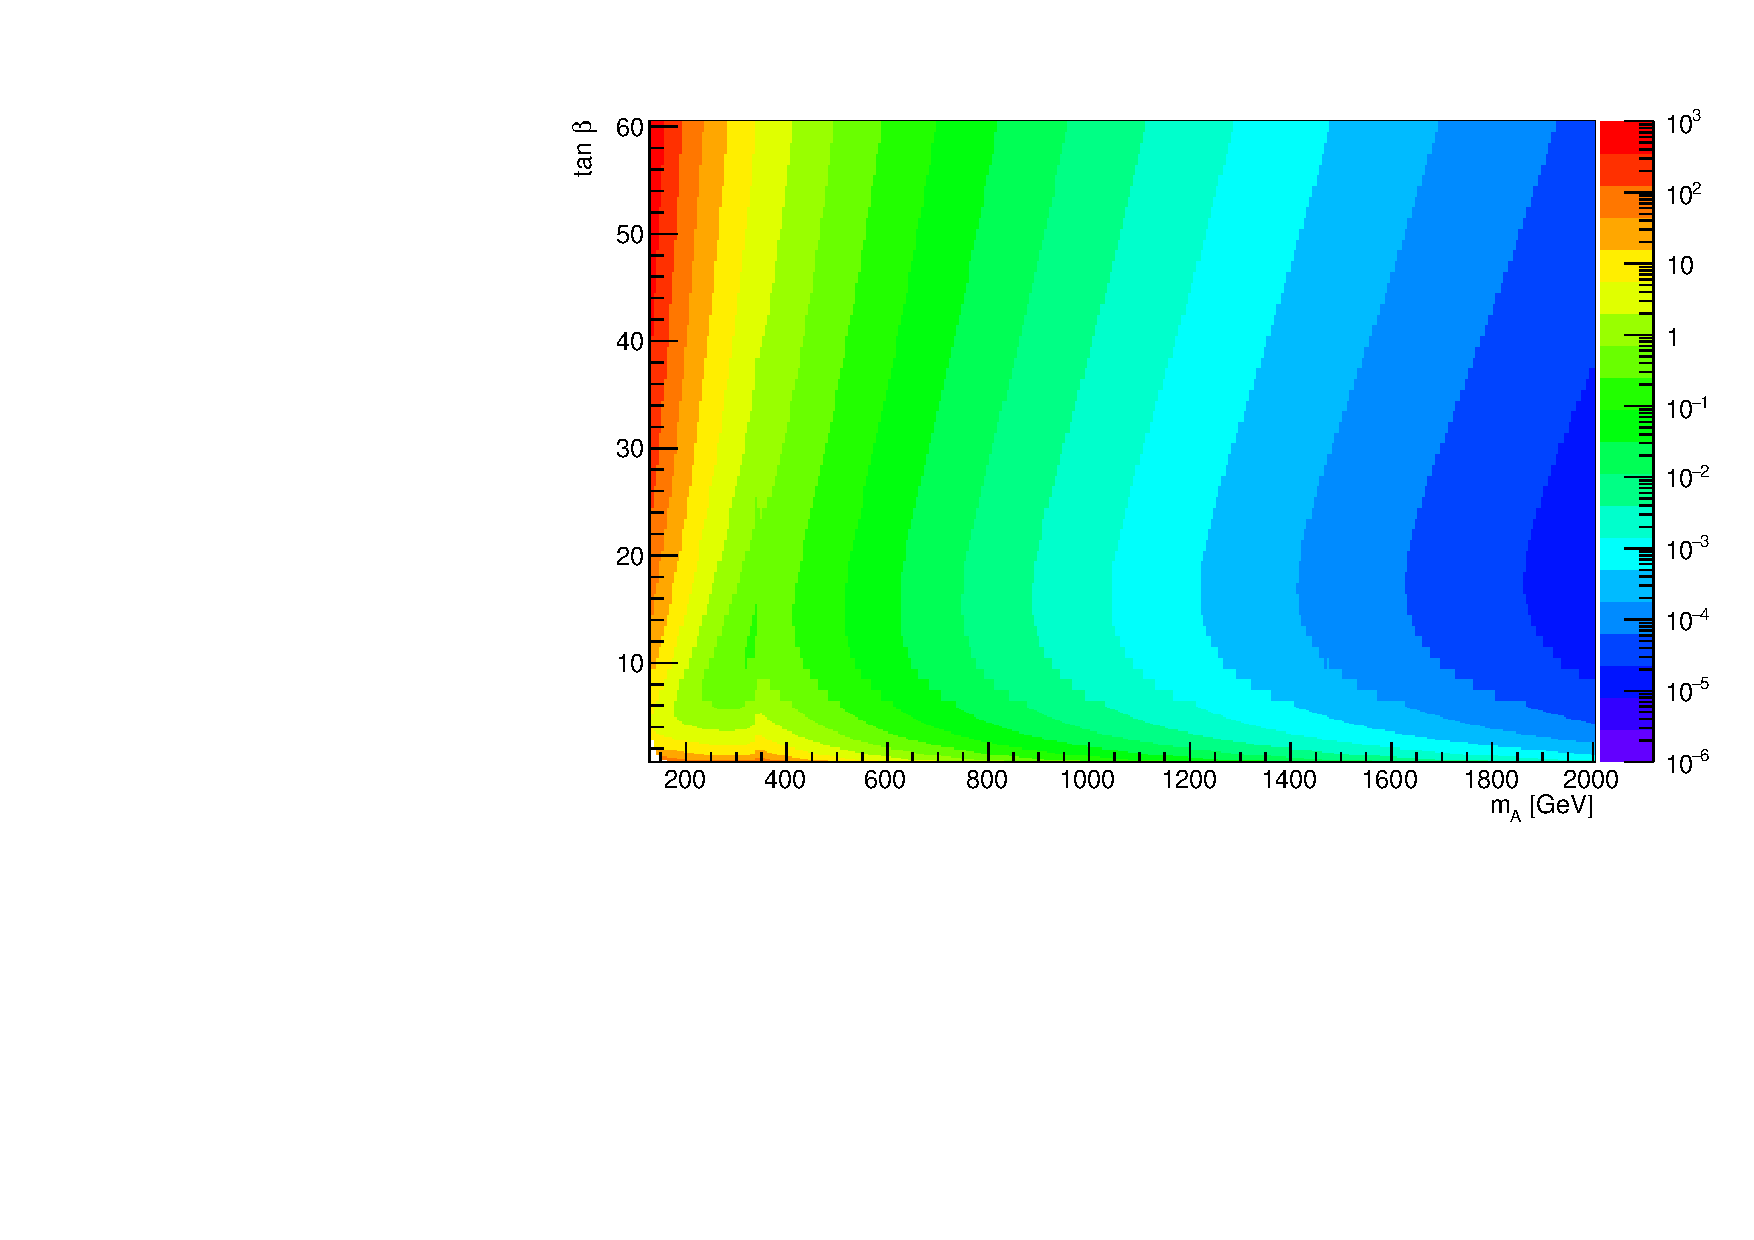
\includegraphics[width=0.5\textwidth]{./Theory/Figures/xsggA_hmssm.pdf}}
%\subfloat[$\sigma(bb\rightarrow bb\PHiggs)$]{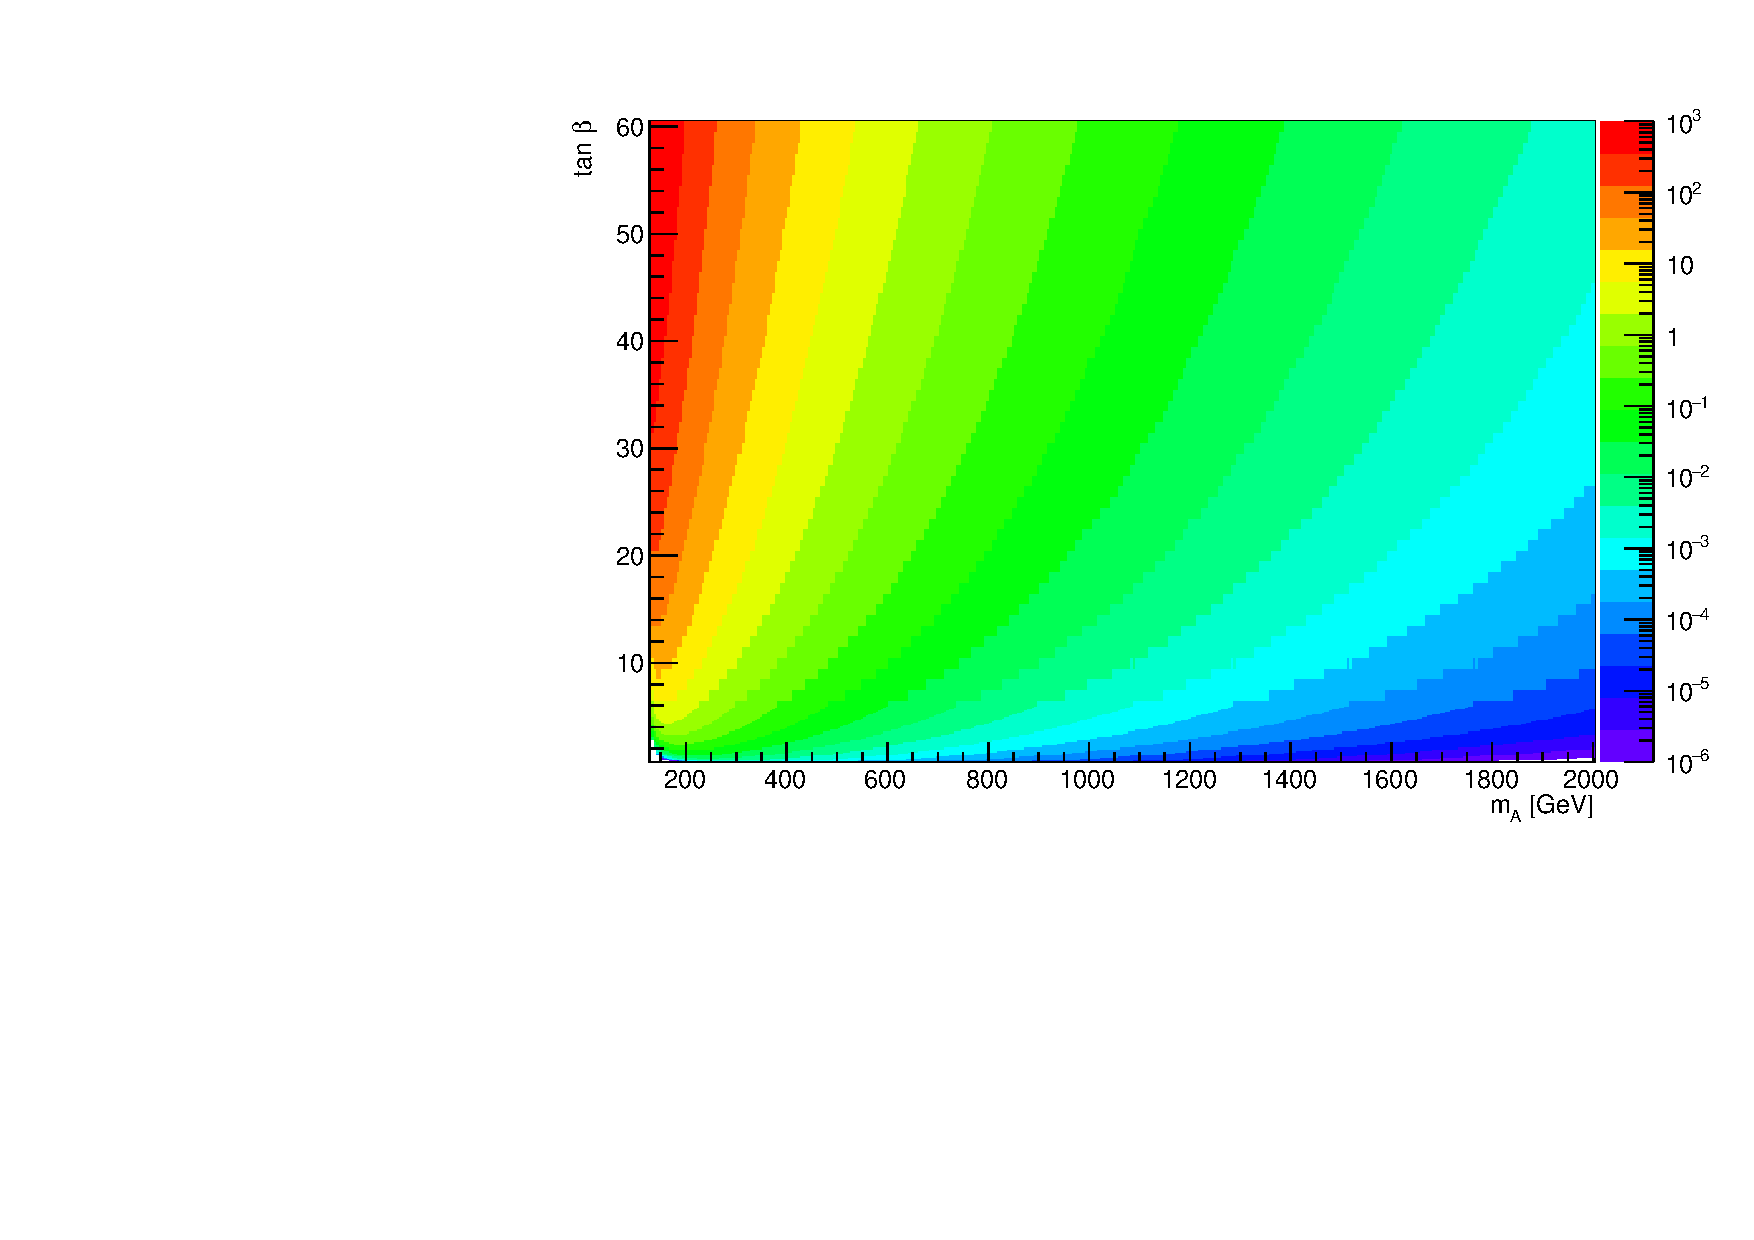
\includegraphics[width=0.5\textwidth]{./Theory/Figures/xsbbH4F_hmssm.pdf}}
%\end{center}
%\caption{Cross-sections at $\sqrt{s}=13$ TeV as a function of
%\mA~and \tanb~ in 
%the hMSSM scenario for (a) gluon fusion production of the \PHiggsps boson and (b)
%b-associated production (four--flavour scheme) of the \PHiggs boson. We can generally see the cross-sections increase
%with growing \tanb, apart from the gluon fusion cross section which decrease with increasing
%\tanb~for low \tanb.}
%\label{fig:hmssm_xs}
%\end{figure}
%\begin{figure}[h!]
%\begin{center}
%\subfloat[BR$(\PHiggs\rightarrow\Pgt\Pgt)$]{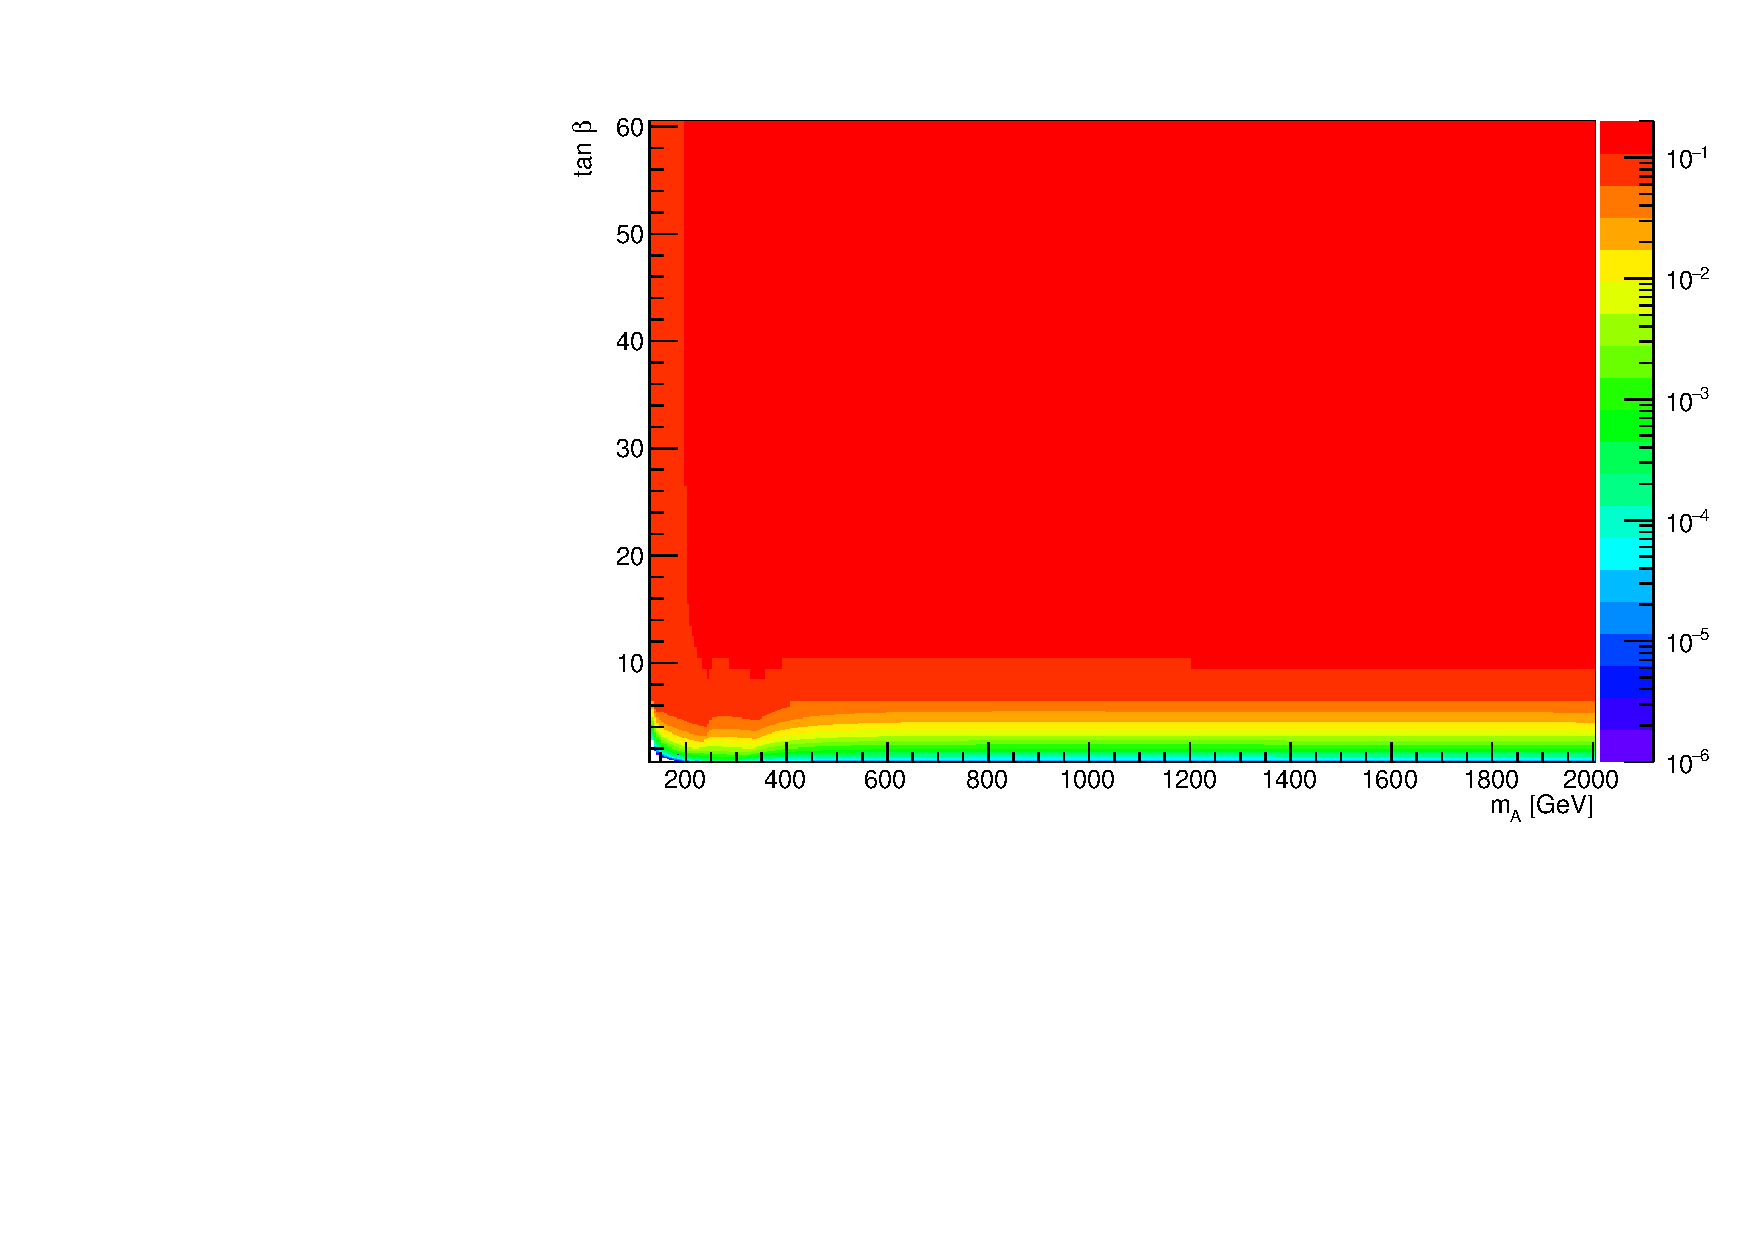
\includegraphics[width=0.5\textwidth]{./Theory/Figures/brHtautau_hmssm.pdf}}
%\subfloat[BR$(\PHiggsps\rightarrow\Pgt\Pgt)$]{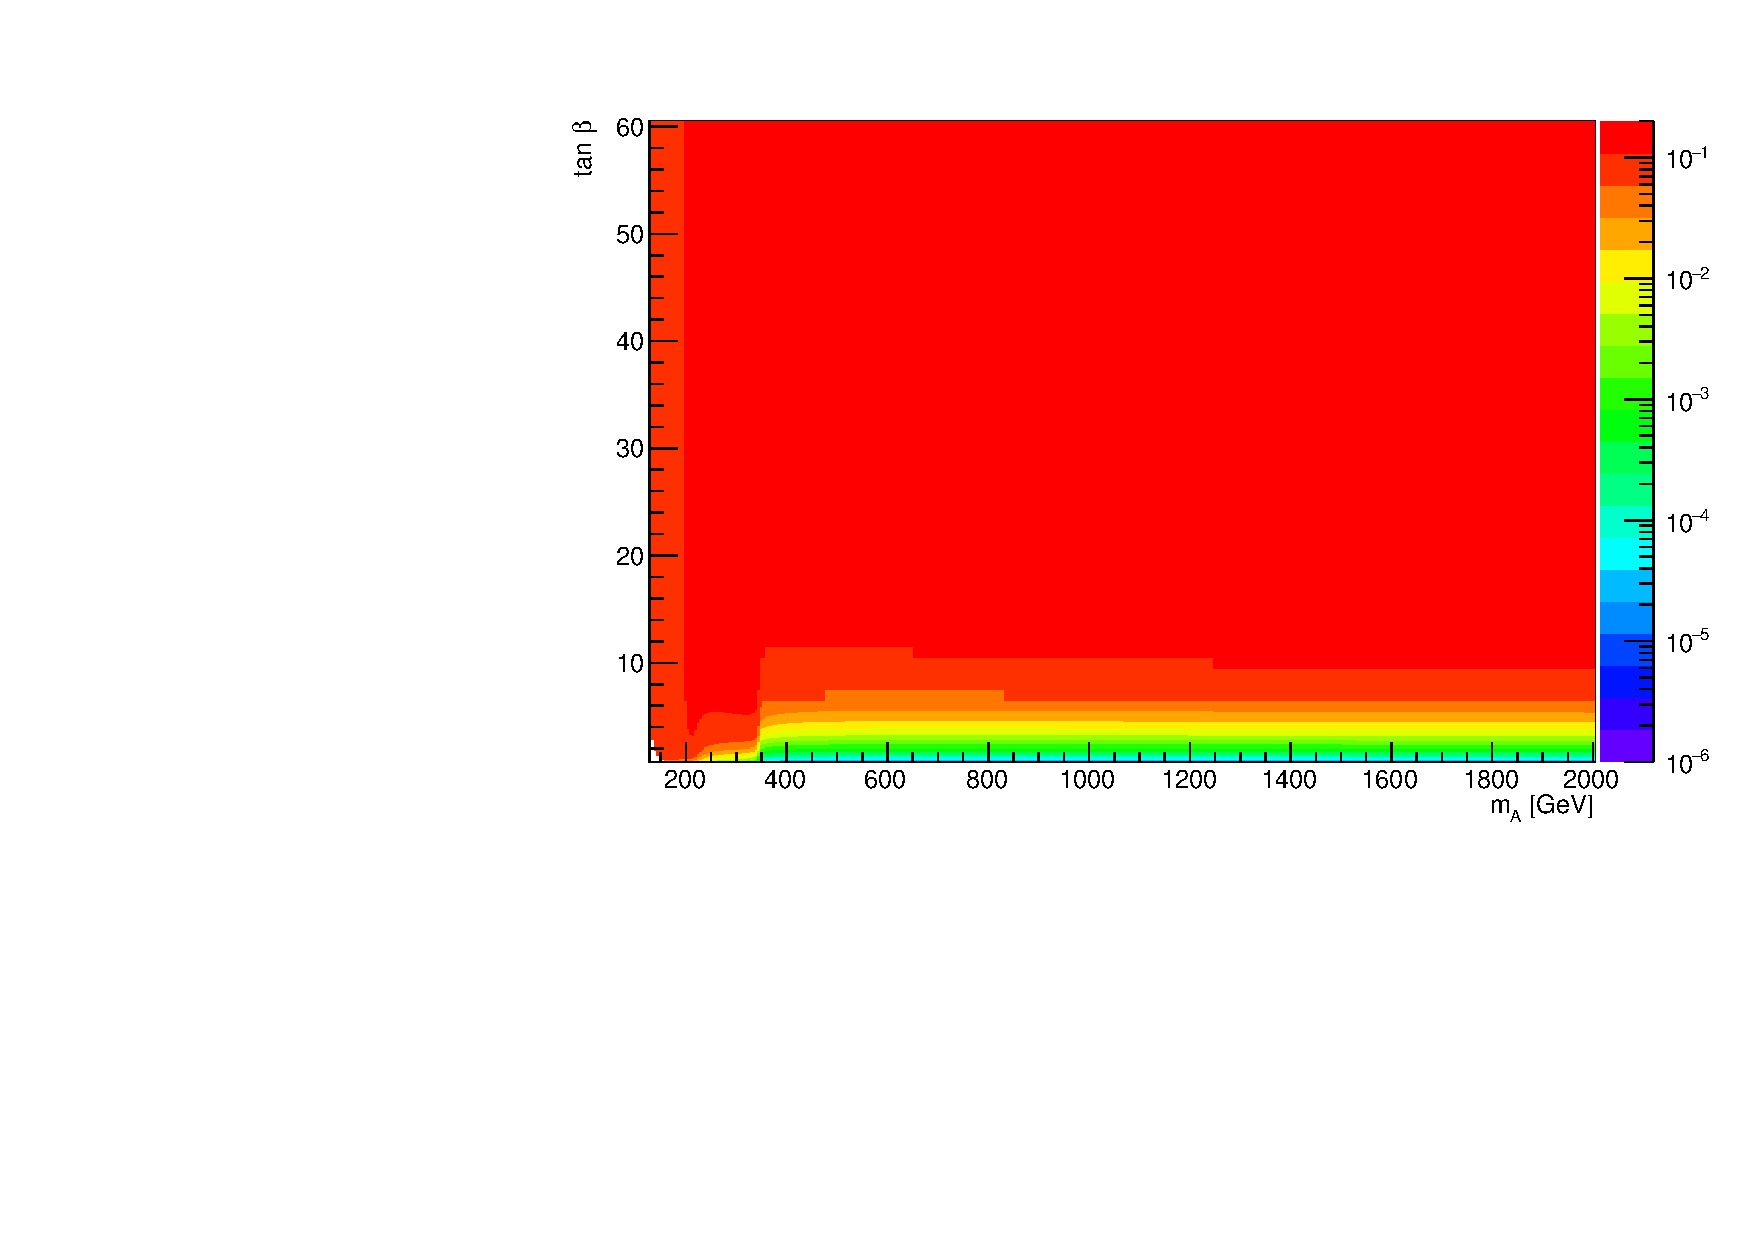
\includegraphics[width=0.5\textwidth]{./Theory/Figures/brAtautau_hmssm.pdf}}
%\end{center}
%\caption{Branching ratios of (a) the \PHiggs boson and (b) the \PHiggsps boson into \tautau. The
%branching ratio is enhanced at high \tanb.} 
%\label{fig:hmssm_brtautau}
%\end{figure}

\section{Status of BSM Higgs boson searches}
\label{sec:theory_BSMH_status}
With the data collected by the \ac{LHC}
experiments up to the end of 2012 many searches for \ac{BSM} Higgs
bosons were performed. Figure \ref{fig:bsm_summary} shows the interpretations
of different searches performed with the \acs{CMS} detector during this period
in the $m_{\PHiggslight}^{\text{mod+}}$ (figure~\ref{fig:bsm_summary}a)
and hMSSM (figure~\ref{fig:bsm_summary}b) scenarios. The direct search for heavier Higgs bosons decaying into pairs
of tau leptons sets the most stringent limits at high \tanb, with searches for 
heavy Higgs bosons decaying to $\Pbottom\Pbottom$ and to $\mu\mu$ both excluding smaller parts of the high-\tanb~region.
Searches for heavy Higgs bosons decaying to $\PW\PW$ and $\PZ\PZ$ are able to exclude part of the low-\tanb~region. In the 
hMSSM scenario searches for \Htohh and \AtoZh can exclude a small area at low \tanb~and between \mA~$=250$--$350\,\GeV$.
The red exclusion contour in figure \ref{fig:bsm_summary}b is the reinterpretation of the analysis presented in
chapter \ref{chap:hhh}.

Since the restart of the \acs{LHC} in 2015 searches for \AHtotautau, setting more stringent limits than those shown in figure \ref{fig:bsm_summary},
have been performed with the \acs{CMS} detector. The results of these searches will be presented in chapter \ref{chap:mssm}. 
Similar searches have been performed by ATLAS \cite{ATLASMSSMtautau2016}. Neutral \ac{BSM} Higgs bosons
are being searched for in other channels too, with some results for decays into $\Ptop\Ptop$ \cite{ATLASHttbar}, 
$\PZ\PZ$ \cite{CMSHZZ2016,ATLASHZZ2016}, and $\PW\PW$ \cite{ATLASHeavyHWW} already public.
In addition, searches for charged
Higgs bosons \cite{ATLASHplustaunu,ATLASHplustb,CMSHplustaunu} and
di-Higgs searches \cite{ATLASHbbgamgam,ATLASHgamgamWW,ATLASHhhbbbb,CMSbbgamgam,CMSHbbtautau,CMSHbbWW}, both in 
various final states, have been performed. %As more data are collected during Run 2 and beyond, the \ac{BSM}
%Higgs sector will continue to be probed.

\begin{figure}[h!]
\begin{center}
\subfloat[$m_{\PHiggslight}^{\text{mod+}}$ scenario]{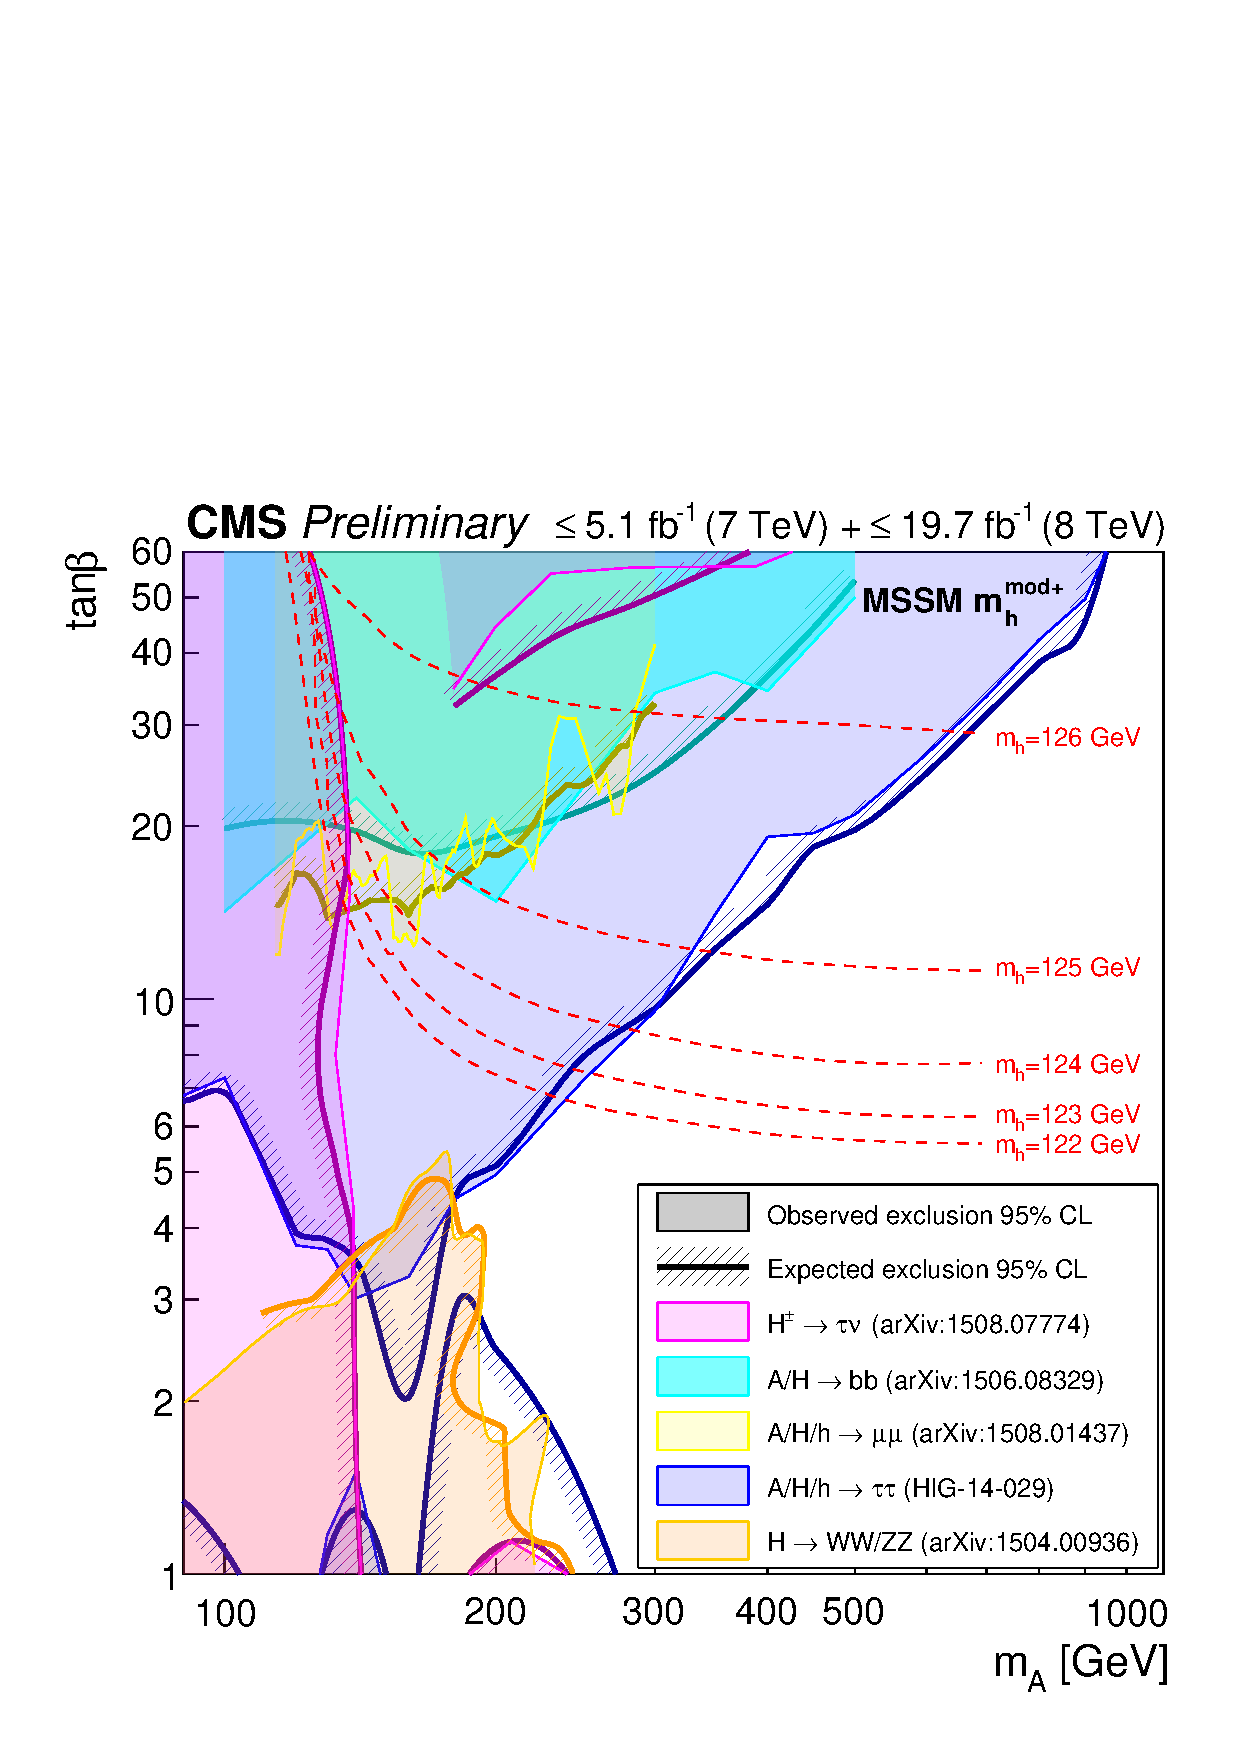
\includegraphics[width=0.5\textwidth]{./Theory/Figures/CMS-PAS-HIG-16-007_Figure_003-a.pdf}}
\subfloat[hMSSM scenario]{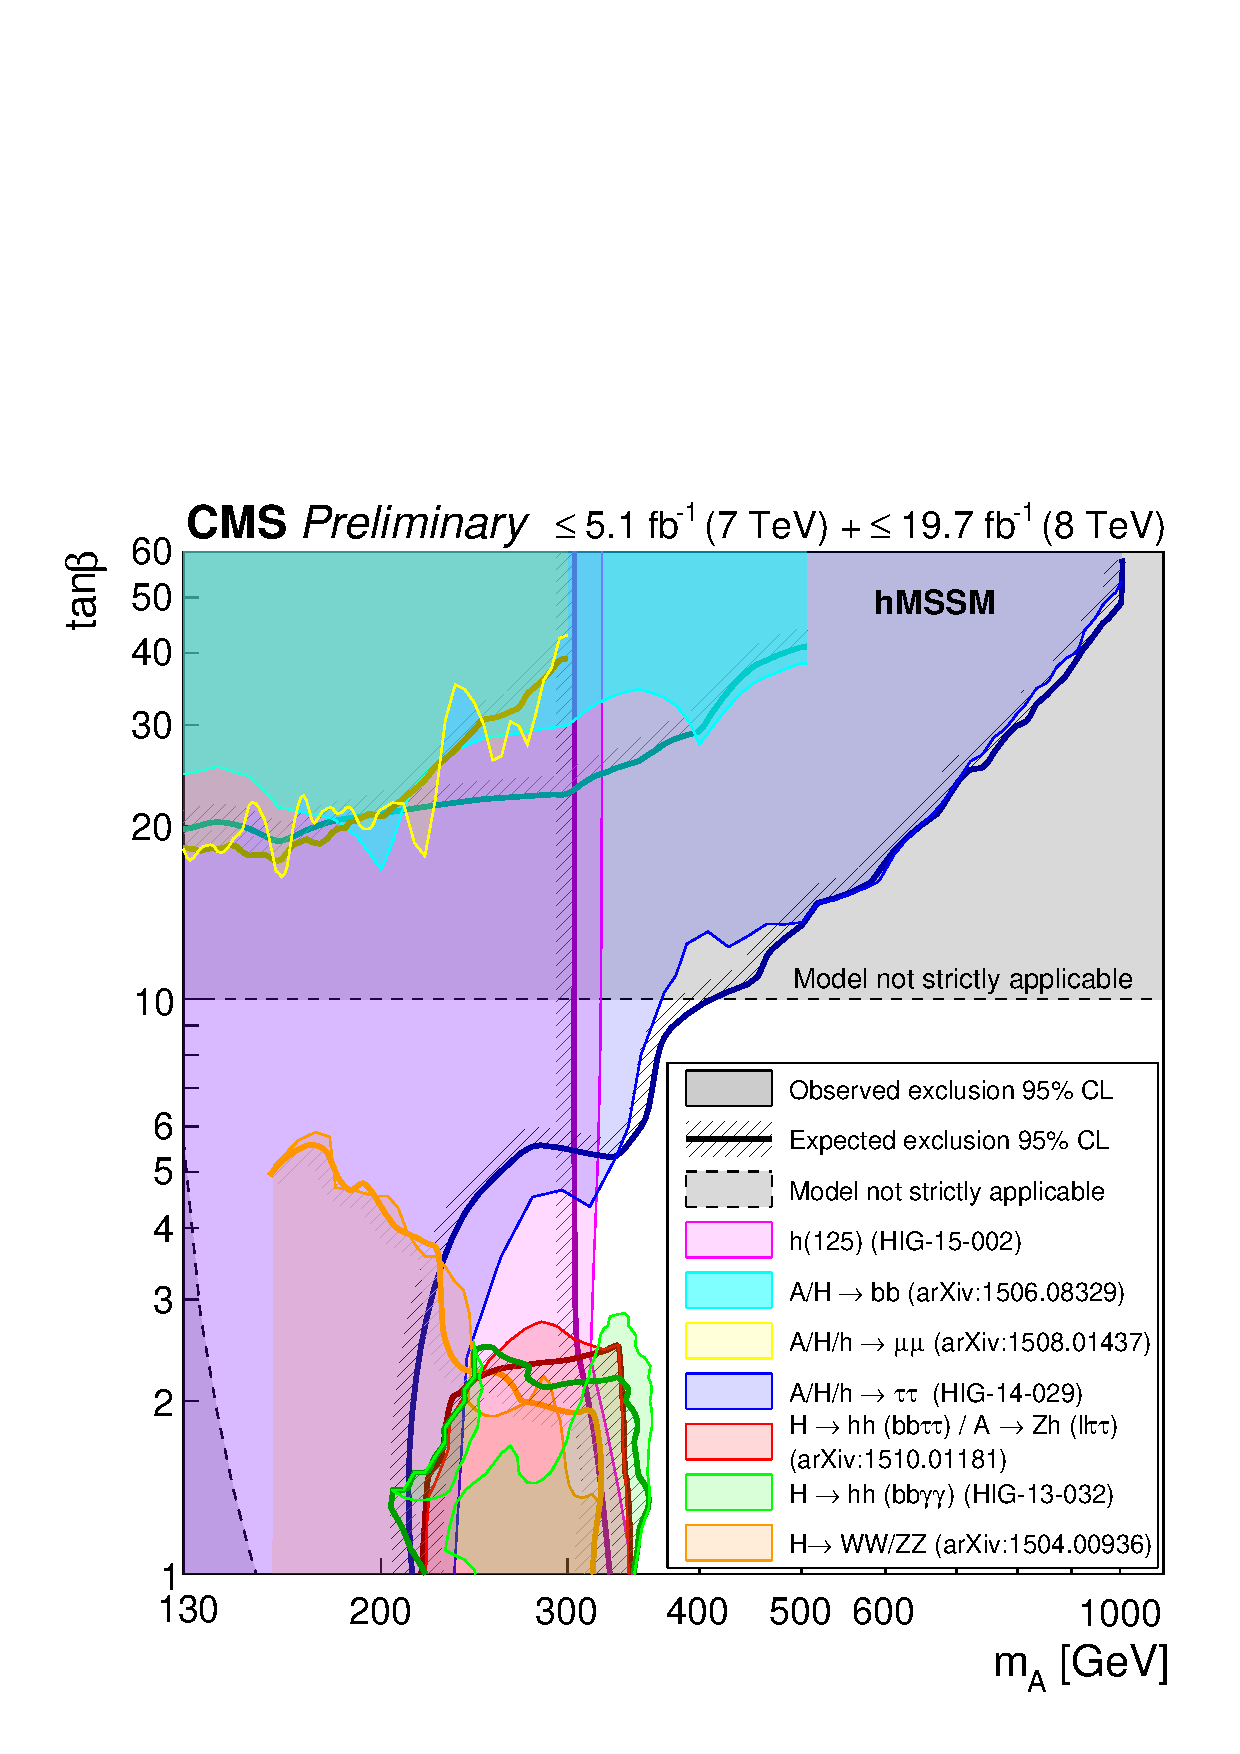
\includegraphics[width=0.5\textwidth]{./Theory/Figures/CMS-PAS-HIG-16-007_Figure_003-b.pdf}}
\end{center}
\caption[Summary of the interpretations of BSM Higgs boson searches using data up to the end of 2012 at CMS in the $m_{\PHiggslight}^{\text{mod+}}$ scenario and the hMSSM scenario.]{Summary of the interpretations of \ac{BSM} Higgs boson searches at \acs{CMS} using data
collected up to the end of 2012 in (a) the $m_{\PHiggslight}^{\text{mod+}}$ and (b) the
hMSSM scenario. The different coloured areas indicate the observed and expected exclusion from different searches in these
scenarios. The results from \ac{MSSM} Higgs boson searches with decays into tau leptons are shown in blue and exclude more of the parameter
space than any of the other searches. The \ac{MSSM} Higgs to $\Pbottom\Pbottom$ (cyan) and Higgs to $\mu\mu$ (yellow) searches are also sensitive in part
of the high-\tanb~region, with searches for Higgs to $\PW\PW$ or $\PZ\PZ$ (orange) providing exclusion power at low \tanb~and low mass. In the $m_{\PHiggslight}^{\text{mod+}}$ 
scenario the charged Higgs to $\Pgt\Pgn$ search (magenta) excludes the low mass region for all values of \tanb. Masses below around $300\,\GeV$ in the 
hMSSM scenario are excluded instead by constraints from \ac{SM} Higgs boson measurements (magenta). In this scenario small
areas of the low-\tanb~region are also excluded by the searches for $\PHiggs\rightarrow \PHiggslight\PHiggslight \rightarrow \Pbottom\Pbottom\tau\tau$ and $\PHiggsps\rightarrow \PZ\PHiggslight \rightarrow \ell\ell\tau\tau$ (red)
and the search for $\PHiggs\rightarrow \PHiggslight\PHiggslight \rightarrow \Pbottom\Pbottom\gamma\gamma$ \cite{CMS-PAS-HIG-16-007}.}
\label{fig:bsm_summary}
\end{figure}



  \chapter{The \acs{LHC} and the \acs{CMS} experiment}
\label{chap:CMSLHC}

\section{The \acs{LHC}}
\label{sec:CMSLHC_LHC}

The \acf{LHC} \cite{lhc-machine}  is a 26.7 km long synchrotron hadron accelerator and collider below the surface of the 
Franco-Swiss border near Geneva. It
is installed in the tunnel that previously housed the Large Electron Positron accelerator
that was operated by \acf{CERN} between 1989 and 2000.

The \ac{LHC} was designed to collide beams of protons with each other at centre-of-mass
energies of up to 14 TeV. It therefore consists of two rings in which the two beams
of protons are individually accelerated. In addition to colliding beams of protons, the \ac{LHC}
is also used for proton--lead and lead--lead collisions.

The \ac{LHC} does not operate on its own, a chain of accelerators leads
the protons into the \ac{LHC}. Figure \ref{fig:lhc_schematic} shows a schematic
of the \ac{CERN} accelerator complex.
\begin{figure}[h!]
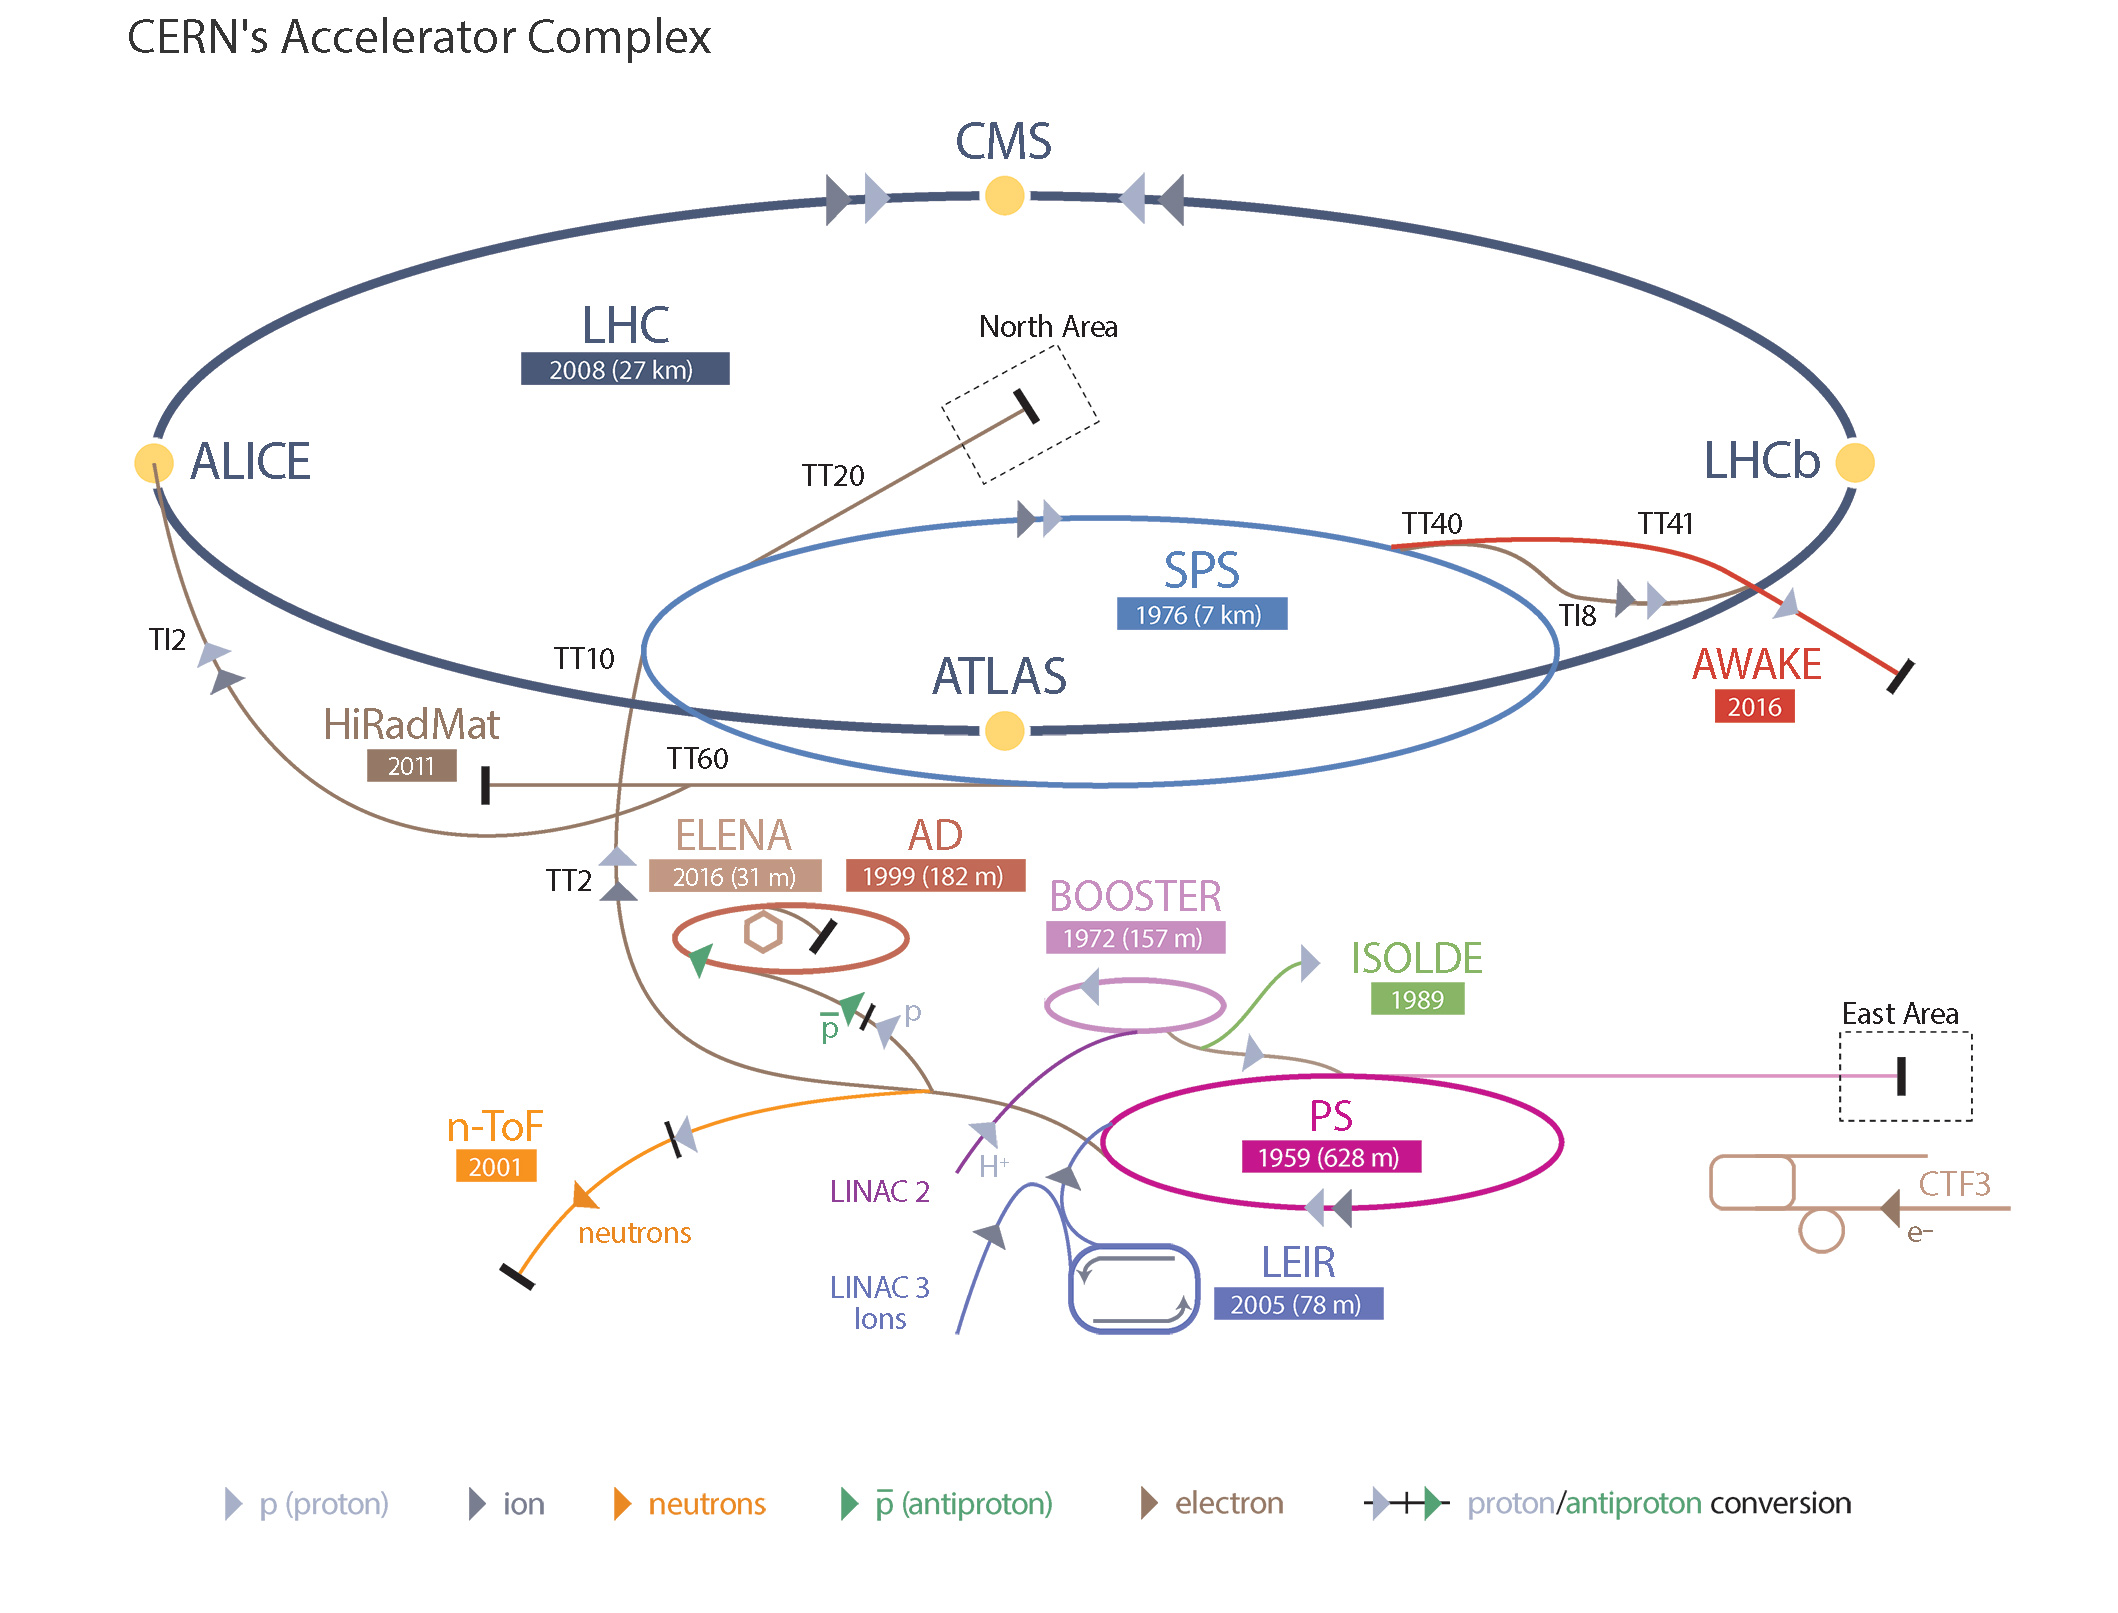
\includegraphics[width=0.8\textwidth]{./Detector/Plots/LHC_default.jpg}
\caption{Schematic of the \ac{CERN} accelerator complex \cite{lhc-schematic}.}
\label{fig:lhc_schematic}
\end{figure}
Protons originate from hydrogen gas, where electrons are stripped off the 
hydrogen atoms using an electric field. The protons then pass through an injector
chain which increases the energy of the protons in several steps. After the protons
are created from the hydrogen gas, they are accelerated to a centre of mass energy of
50 MeV in the Linac2 linear accelerator. They are then passed on to the
\acf{PSB} which accelerates the protons until they reach a centre of mass energy of 1.4 GeV.
The next accelerator in the chain, the \acf{PS}, further accelerates the protons to 25 GeV,
with the \acf{SPS} bringing the energy up to 450 GeV. When this energy has been 
reached the protons are injected into the \ac{LHC}, where they are further accelerated to 
the required centre of mass energy. The beams collide at four points
around the ring, where the collisions are recorded by the ATLAS\cite{atlas-jinst}, 
CMS\cite{cms-jinst}, ALICE\cite{alice-jinst}, and LHCb\cite{lhcb-jinst} detectors.

The processes the \ac{LHC} was built to study have a small cross-section
compared with the total proton-proton inelastic cross-section, as seen from figure
\ref{fig:stirling_xs}. For example, the production cross-section of the
standard model Higgs boson is 9-10 orders of magniuted smaller than the total p--p cross section.

\begin{figure}[h!]
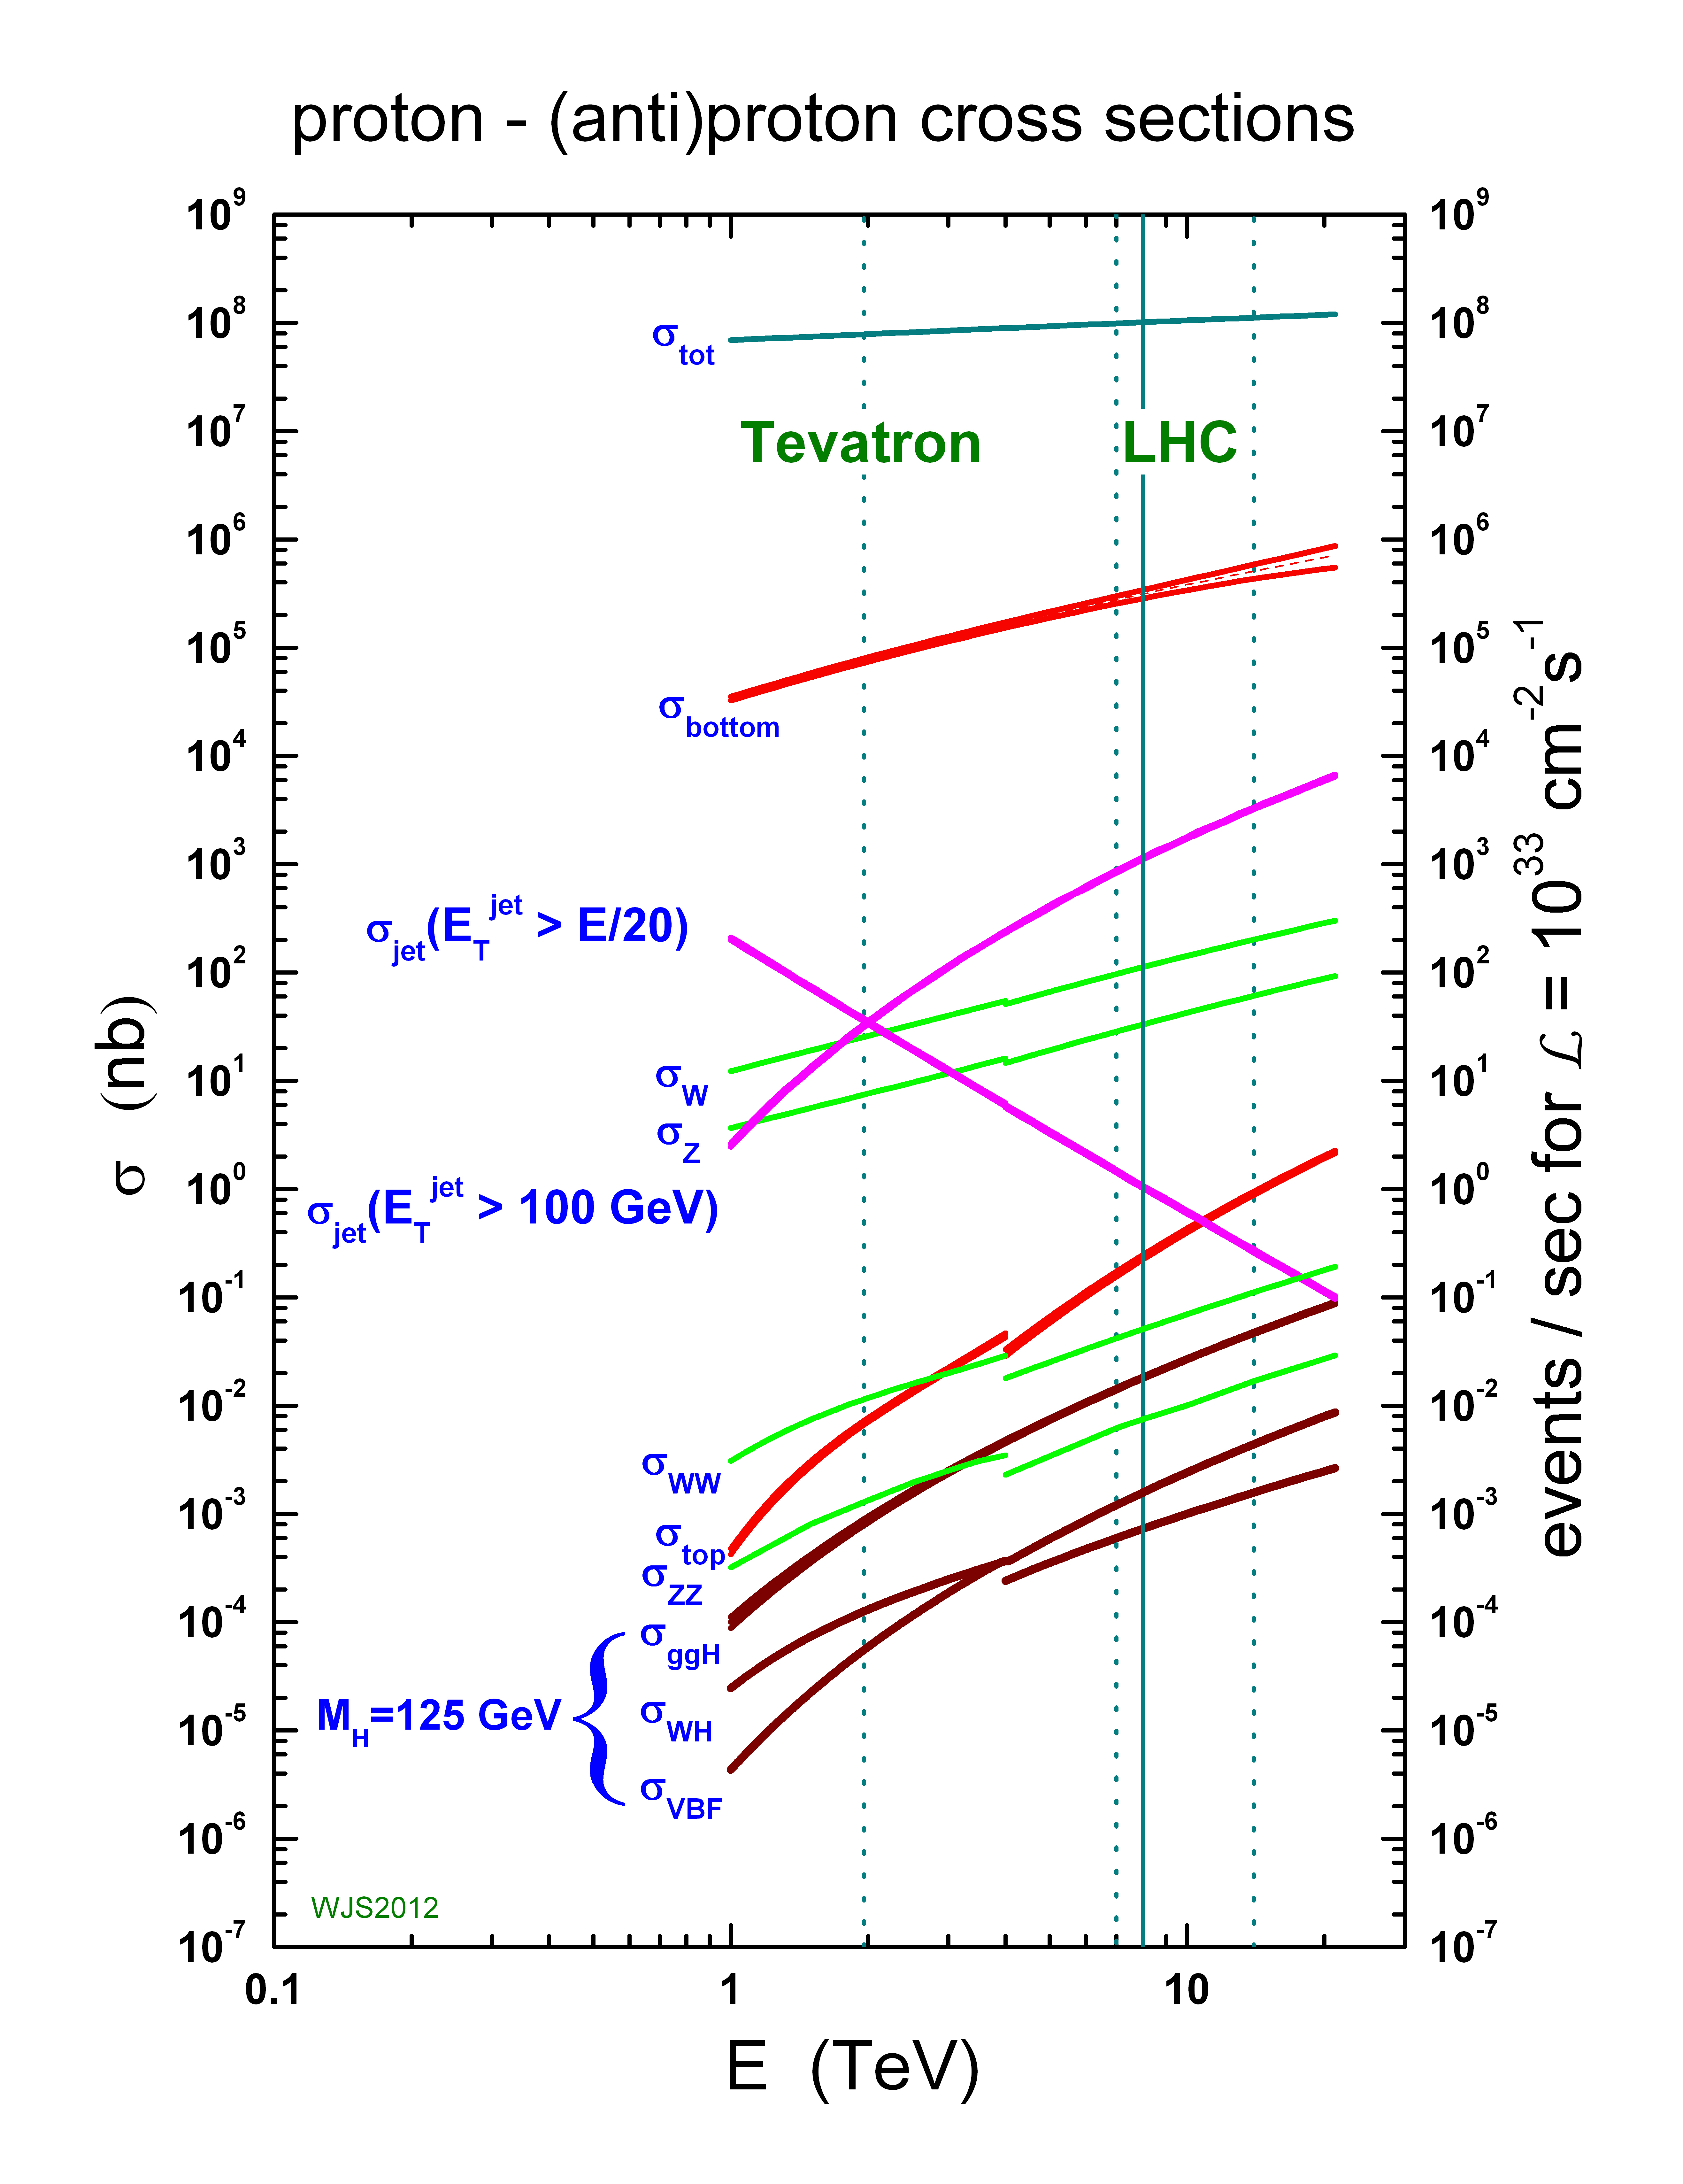
\includegraphics[width=0.5\textwidth]{./Detector/Plots/crosssections2013.jpg}
\caption{Total proton-proton cross section, and the cross-sections
for several processes studied at the LHC \cite{stirling-crosssection}.
The cross sections of these processes
are often many orders of magnitude smaller than the total p--p cross section.}
\label{fig:stirling_xs}
\end{figure}

In order to be able to study these relatively rare processes, 
the LHC operates at high instantaneous luminosity, defined as in equation
\ref{eqn:CMSLHC_luminosity}. 
\begin{equation}\label{eqn:CMSLHC_luminosity}
\mathcal{L} = \frac{N_b^2n_bf_{\text{rev}}\gamma}{4\pi\epsilon_n\beta^{*}}F
\end{equation}

In this equation, $N_b$ is the number of protons per bunch, $n_b$ the number of
bunches per beam, $f_{\text{rev}}$ the revolution frequency, $\gamma$ the 
Lorentz factor, $\epsilon_n$ the normalised beam
emittance, $\beta^{*}$ the $\beta$-function at the interaction point and F a reduction
factor due to the crossing angle. 

After an initial testing phase, the \ac{LHC} began its first physics run in May 2010 with 
a centre of mass energy of 7 TeV. The CMS experiment recorded an integrated luminosity of 45 pb$^{-1}$
during 2010. In 2011 the \ac{LHC} continued operating at a centre-of-mass energy of 7 TeV, delivering an integrated 
luminosity of 6.1 fb$^{-1}$ to the CMS experiment. The centre of mass energy was increased to 8 TeV
for the 2012 data-taking period, during which an integrated luminosity of 23.3 fb$^{-1}$ was delivered.
This completed Run 1 of the \ac{LHC}, after which the 2-year \ac{LS1} was used to 
upgrade the LHC and the detectors for collisions at a centre of mass energy of 13 TeV.

In April 2015 the \ac{LHC} restarted with collisions at a centre-of-mass energy of 13 TeV, and during 
this year 4.2 fb$^{-1}$ was delivered. Collisions at a centre-of-mass energy of 13 TeV continued
in 2016, when a total of 41.1 fb$^{-1}$ was delivered. 
The integrated luminosity as a function of time is shown in figure \ref{fig:CMSLHC_intlumi},
separated by running year.

\begin{figure}[h!]
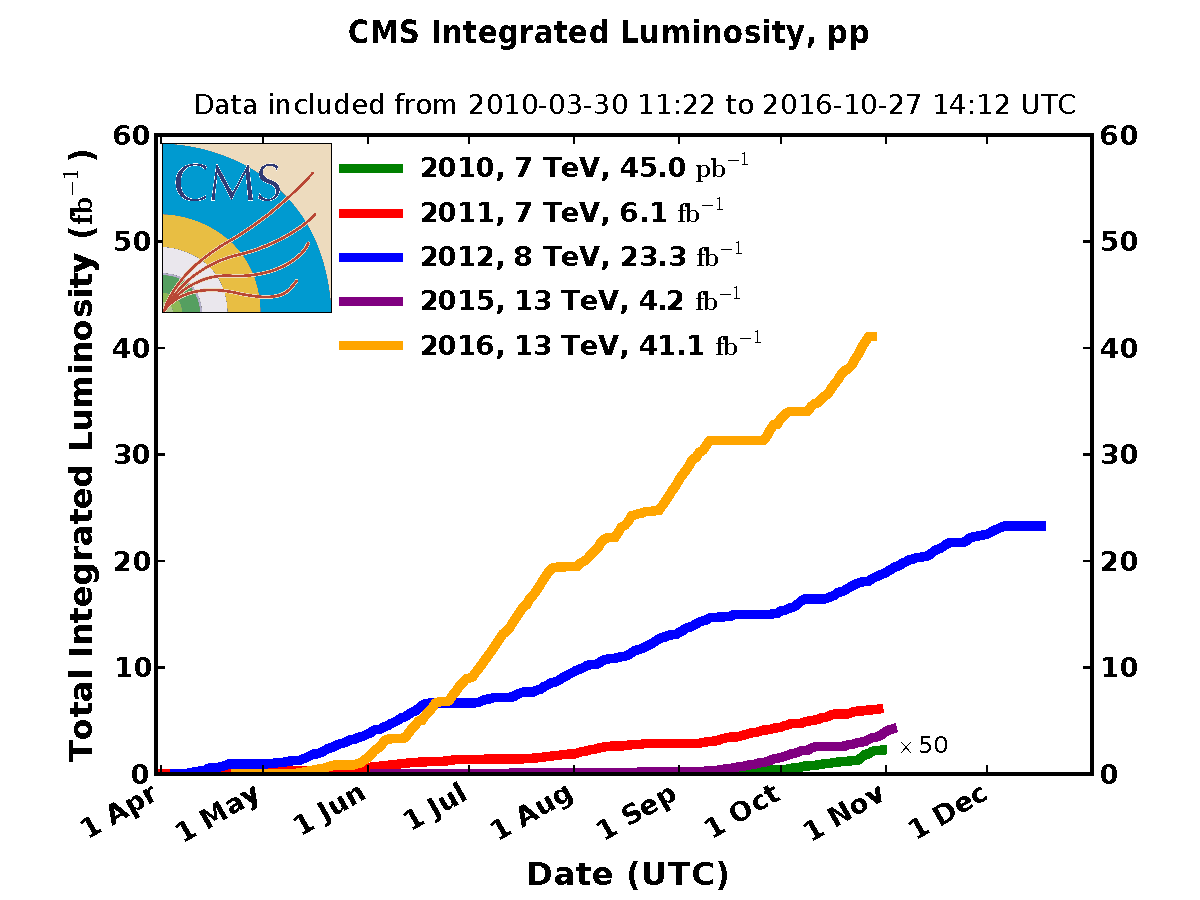
\includegraphics[width=0.85\textwidth]{./Detector/Plots/int_lumi_cumulative_pp_2.pdf}
\caption{Cumulative integrated luminosity for p--p collisions at the LHC, separated
by running year \cite{cms-lumi-public}.}
\label{fig:CMSLHC_intlumi}
\end{figure}

The data-taking efficiency of CMS is not 100\%, for example the detector might be
switched off for part of the time collisions are ongoing. In 2012, the data-taking 
efficiency was 93.5\%, in 2015 it was 90.3\% and in 2016 it was 92.4 \%

From all of the data that is recorded, a subset is used for analyses. Data is 
certified as good for use in analyses if it is known that all relevant subdetectors
were functioning correctly. The certification efficiency in 2012 was 90.4\%,
leading to an integrated luminosity of 19.7 fb$^{-1}$ for which all subdetectors
were working well, in 2015 it was 60.4 \%, leading to 2.3 fb$^{-1}$ of analysable data
for which the full detector was operational. An additional 0.6 fb$^{-1}$ was taken
with the magnet switched off. The certification efficiency for the full 2016 p--p running period was 95.4\%.

The \ac{LHC} was designed for a nominal
peak luminosity of $10^{32}$cm$^{-2}$s$^{-1}$ for proton-proton collisions. In 2012 peak
luminosities of $7.7*10^{33}$cm$^{-2}$s$^{-1}$ were reached, with the peak luminosity in
2015 being $5.1*10^{33}$cm$^{-2}$s$^{-1}$. Since July 2016
the \ac{LHC} has been operating at instantaneous luminosities upwards of the 
design luminosity, with peak luminosities of $1.5*10^{32}$cm$^{-2}$s$^{-1}$ reached
in October 2016.

Due to the high operating luminosity, multiple proton-proton collisions per 
bunch crossing are likely to occur. The average number of interactions
per bunch crossing is X in 2012, Y in 2015, Z in 2016. Additional 
interactions on top of events of interest are referred to as pile-up.

\section{The \acs{CMS} detector}
\label{sec:CMSLHC_CMS}
To meet the demands of the \ac{LHC} physics programme, the
 \ac{CMS} detector was designed to be very perfomant in searches
for physics at the TeV scale and to be able to 
function in the challenging high-luminosity environment.
The detector is 21.6 m long, 14.6 m in diameter, and weighs
12500 tonnes \cite{cms-jinst}. It consists of several subdetectors, as illustrated
in figure \ref{fig:cms_detector}. Surrounding the interaction
point is the silicon tracker, a cylinder 5.8 m in lenght and 2.6 m in 
diameter. Surrounding the silicon tracker
the lead-tungstate \ac{ECAL} is found, which in turn is enclosed
by a brass scintilator \ac{HCAL}. 

The tracking and calorimeter systems are surrounded by a superconducting
solenoid, 13 meter long and 6 meter in diameter and operating at 3.8 Tesla.
Charged particles are bent in this magnetic field, allowing for precise 
measurement of their momentum. Gaseous muon detectors are embedded in the 
iron return yoke of the solenoid.

For the measurement of physical quantities, \ac{CMS} uses a coordinate
system with the origin centred at the nominal collision point
inside the experiment. The y-axis points vertically upward, the x-axis
points radially inward toward the centre of the \ac{LHC} ring. The z-axis
points along the beam direction. As such the transverse momentum and energy, 
\pT and \ET are measured from the x- and y- components of the momentum and energy.
The azimuthal angle $\phi$ is measured in the x-y plane with respect to the x-axis, 
the polar angle $\theta$ measured with respect to the z-axis. A coordinate
more frequently used than the polar angle is the pseudorapidity $\eta = -\ln{[\tan{\frac{\theta}{2}}]}$.
Distances in the $\eta-\phi$ plane are given as $\Delta R = \sqrt{(\Delta\eta)^2+(\Delta\phi)^2}$. 

The subsystems of the \ac{CMS} detector will be described in more detail in the 
next sections.

\begin{figure}[h!]
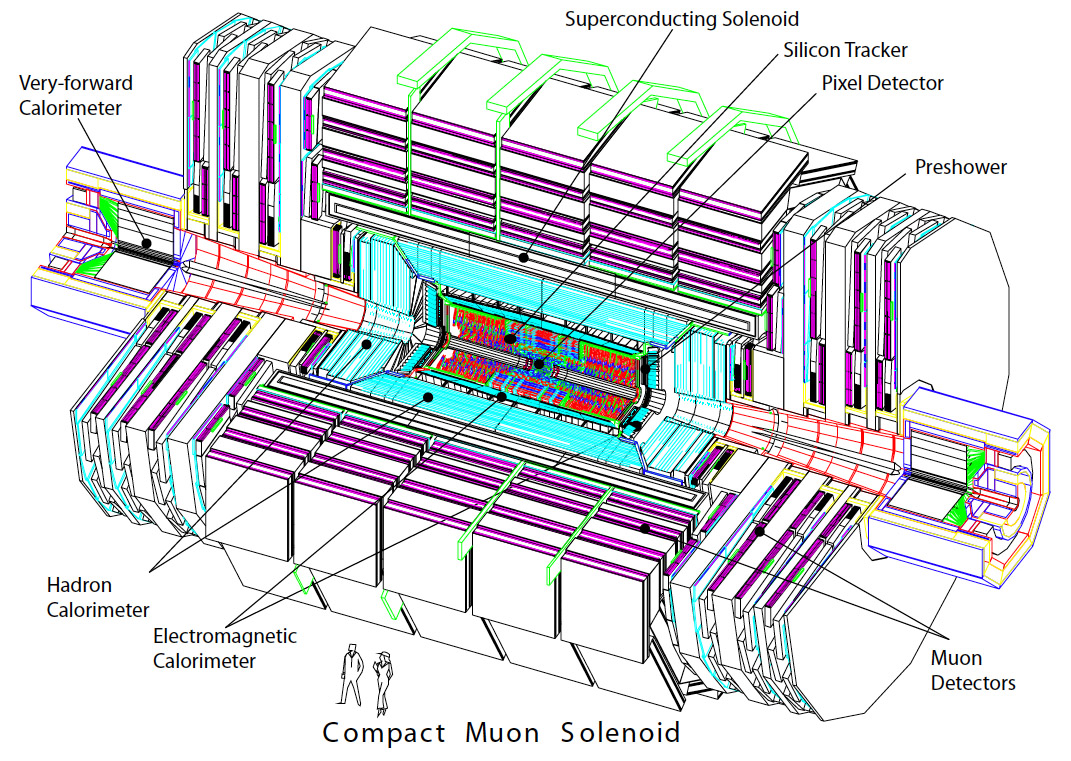
\includegraphics[width=0.8\textwidth]{./Detector/Plots/cms.png}
\caption{A blow-up view of the \ac{CMS} detector \cite{cms-jinst}, indicating the
different sub-parts of the detector.}
\label{fig:cms_detector}
\end{figure}

\subsection{Tracker}
\label{sec:CMSLHC_CMS_tracker}
The tracker \cite{cms-jinst} is the subdetector closest to the interaction point. It
is used for accurate reconstruction of charged particle trajectories and 
the precise reconstruction of secondary vertices, which are important to be
able to indentify heavy-flavour particles. This means a small impact parameter
resolution needs to be achieved, for which a highly granular system is required. 
Due to the large number of particles emerging from 
each collision, an average of 1000 per bunch crossing (every 25 ns) at LHC design operation, the 
system also needs to be fast-responding in order to reconstruct trajectories accurately.
At the same time, this large particle flux calls for a 
radiation-hard design that is able to survive in this harsh environment
for a longer period of time. These requirements motivate the use of a silicon tracking
system. When a charged particle passes through the silicon, an electron-hole pair
is created, which drift under an applied electric field and produce a current
that can be read out. %LEARN A BIT MORE ABOUT THIS

The tracker provides coverage up to $|\eta| < 2.5$ and consists of
several different components. A schematic of the tracking detector is given
in figure \ref{fig:CMS_tracker}. The part of the tracking system
closest to the interaction point is the silicon pixel detector, which 
consists of 3 layers of pixels in the barrel of the detector, with 
2 pixel endcap disks. The barrel layers sit at radii of 4.4, 7.3 and 10.2 cm 
and extend up to $z=\pm 26.5$ cm, with the disks placed at $z=\pm 34.5$ cm and
$z=\pm 46.5$ cm. The pixel detector consists of 66 million silicon pixels, each
$100 \mu m \times 150 \mu m$ in size. The choice of this pixel size is driven
by the achievable spatial resolution, which is $15-20 \mu m$ in the $r$ and $z$ directions.
This allows for 3D vertex reconstruction. With this layout, the pixel tracker
provides 3 precise position measurements along each charged particle trajectory.


\begin{figure}[h!]
\begin{center}
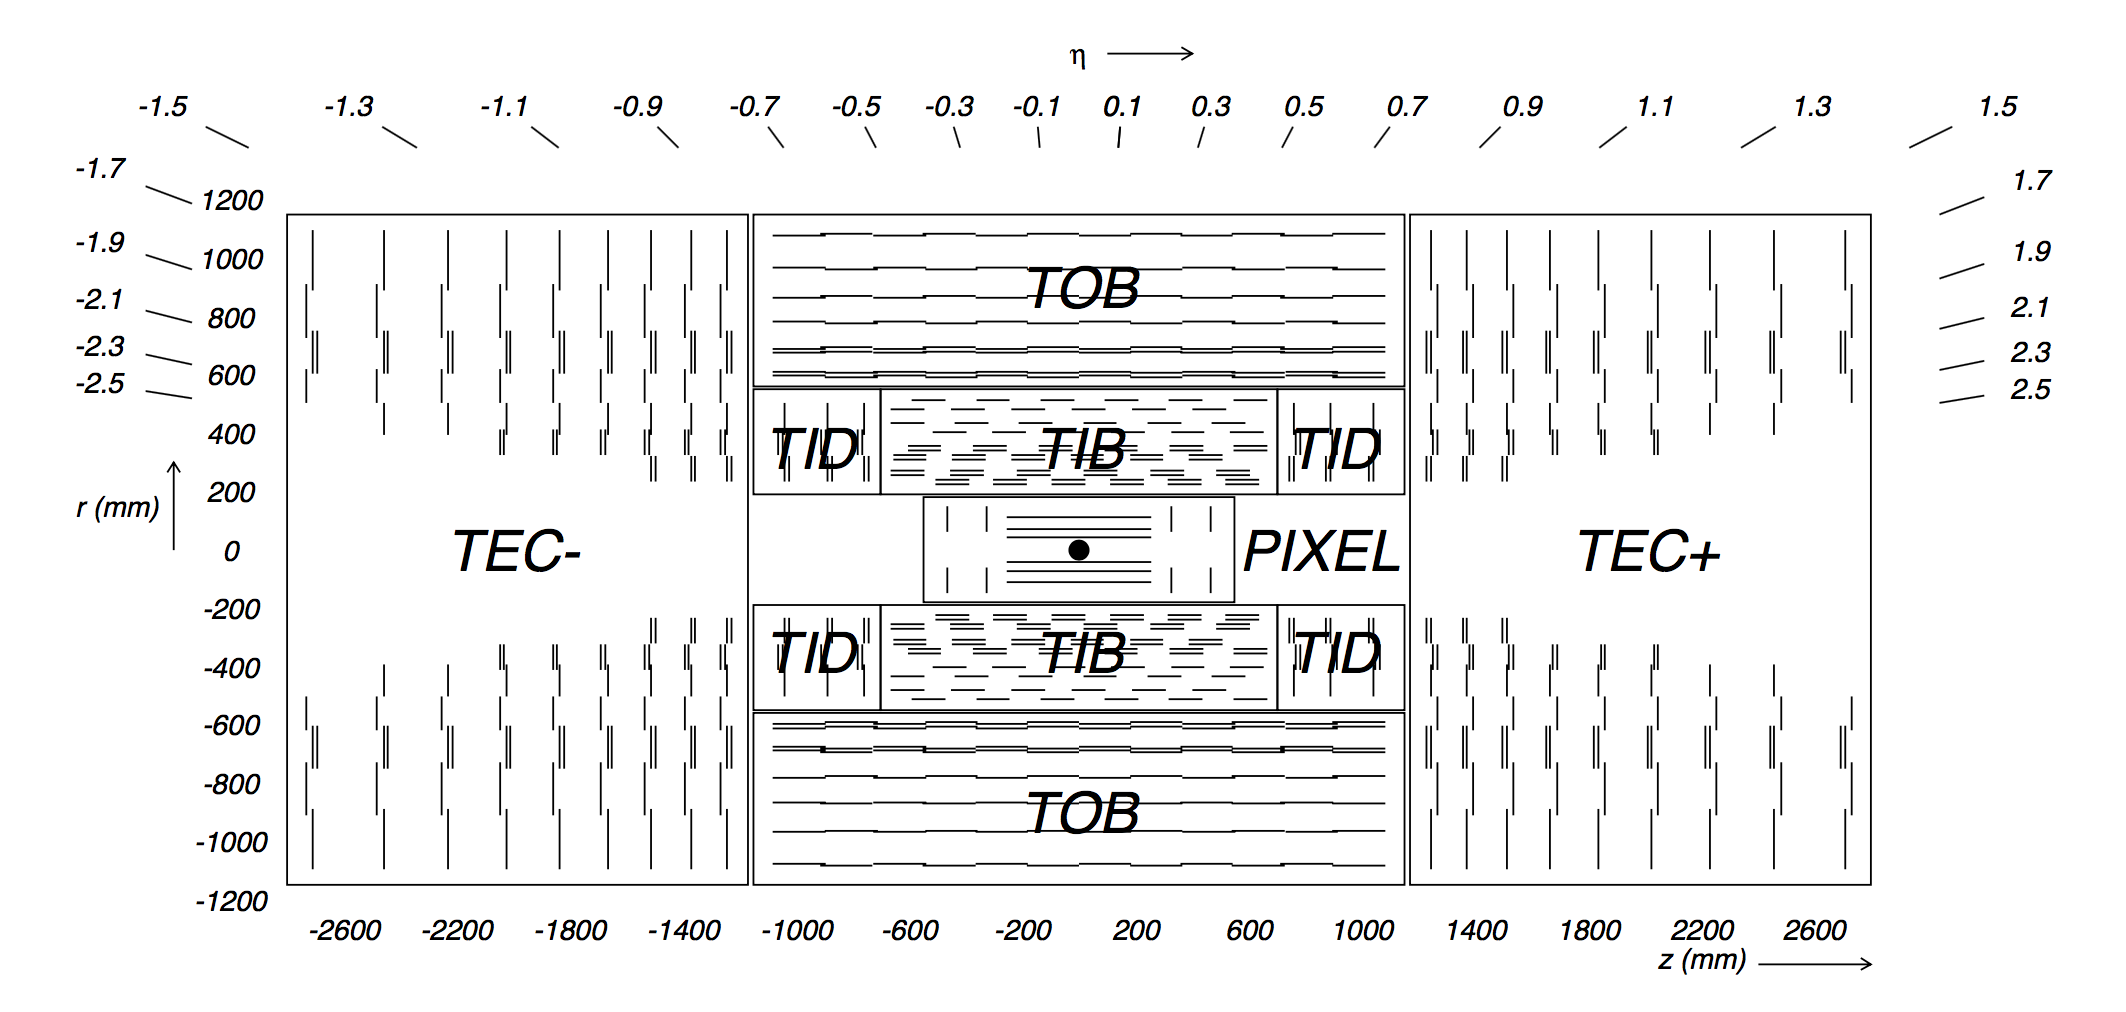
\includegraphics[width=0.9\textwidth]{./Detector/Plots/Tracker.png}
\caption{Schematic of the CMS tracker in the r-z plane, indicating the
positions of the pixel and strip detectors \cite{cms-jinst}. Each line 
on the plot represents a detector module}
\label{fig:CMS_tracker}
\end{center}
\end{figure}


Beyond the pixel detector the tracking system is made up of a silicon
strip detector consisting of over 9 million multiple different subsystems. The first part of the
silicon strip tracker consists of \ac{TIB} and \ac{TID}, providing 4 layers of
silicon strip detectors in the barrel plus 3 disks at both ends. These two systems
extend out towards a radius of 55 cm. The barrel layers and disks each consist
of silicon strips which are 10 cm long, $80-141\mu m$ wide and $320 \mu m$ thick. The \ac{TIB} and \ac{TID}
provide 4 measurements of the $r-\phi$ position  with a resolution of 23-35 $\mu m$.
The \ac{TIB} and \ac{TID} are surrounded by the \ac{TOB}, which consists of 6 layers of silicon strip sensors extending
up to an outer radius of 116 cm and up to $z=\pm 118$ cm. The strips in the \ac{TOB} are 500 $\mu m$ thick, around 25 cm long and 122-183 $\mu m$ 
wide and this subdetector provides 6 measurements of $r$ and $\phi$, with a resolution
of 35-53 $\mu m$. Beyond the z-range covered by the \ac{TOB}, coverage is provided by the \ac{TEC},
consisting of 9 disks of strips.In the \ac{TEC}, the thickness ranges from 320-500 $\mu m$ and the the strip width ranges from $97-184 \mu m$.
In this way this part of the system provides up to 9 $\phi$ measurements.

Some of the strip modules in the detector carry a second strip detector module mounted back-to-back with a stereo angle %FIXME WTF?
of 100 mrad, in order to provide measurements of the $z-$ coordinate in the barrel. This is achieved with a resolution of 230-530 $\mu m$.

The pixel tracker will be upgraded during the extended year-end technical stop in early 2017. %or just replaced?


\subsection{\acl{ECAL}}
\label{sec:CMSLHC_CMS_ecal}
The \ac{ECAL} \cite{cms-jinst} is a hermetic homogeneous calorimeter
made of nearly 76000 lead tungstate (PbWO$_4$) crystals. It has very
good energy resolution, is highly granular and fast-responding, which
are all needed to be able to detect $H\rightarrow \gamma\gamma$ decays.

Despite being further away from the interaction
point than the tracker, the materials in other parts of the detector
still need to be radiation hard. In order to be able to place
the calorimeters inside the bore of the solenoid, a compact \ac{ECAL}
had to be constructed, and to provide excellent resolution a 
highly granular system had to be designed. The lead tungstate crystals have a 
radiation length of 0.89 cm, a Moli\'ere radius of 2.2 cm, and 80\% of the light
from the crystals is emitted in 25 ns. This short radiation
length, small Moli\'ere radius and short scintillation decay time combined
with the radiation hardness of the material motivate the choice of lead tungstate. 

%Moliere radius: characteristic constant of a material giving scale of transverse dimenstion
%of fully contained EM showers. It is the radius of a cylinder containing on average 
%90pct of the shower's energy deposition. Related to radiation length as 
%molrad approx 0.0265X0 (Z+1.2) with Z the atomic number.
%Radiation length: mean distance over which a high energy electron
%loses all but 1/e of its energy by bremmstrahlung and 7/9 of th emean free path for pair production by 
%a high energy photon.

When a high energy electron or photon enters a crystal, it starts a
shower producing a cascade of lower energy particles. Electrons lose
energy through bremsstrahlung, with photons undergoing $\Pe^+ \Pe^-$ 
pair production. The shower continues until the photon energy drops below the 
$\Pe^+\Pe^-$ pair production threshold, and ionisation 
starts to dominate for electrons. The shower ionises the crystals, 
which return to their normal state by emitting scintillation light. 
As the crystals are 25.8 radiation lengths long, most of the shower
is contained inside them.

Figure \ref{fig:CMS_ECAL} shows a schematic of the \ac{ECAL}, indicating
the geometry. The \ac{ECAL} consists of different subsystems. The \ac{EB} 
covers the pseudorapidity range up to $|\eta|<1.479$, with
crystals of $0.0174 \times 0.0174$ in $\eta - \phi$. The \ac{EE}
provides coverage beyond the range of the \ac{EB}, up to $|\eta|<3.0$
Each endcap is divided into two halves. In front of the endcaps 
the preshower detectors, covering $1.653<|\eta|<2.6$ is a sampling
calorimeter whose main use is to indentify neutral pions in the endcaps. Additionally
it helps electron identification and improves the resolution
of position determination. Each of the two preshower detectors consist
of two layers of lead radiators to initiate the shower, with silicon sensors
placed after each layer of radiators to measure the deposited energy. The 
total thickness of the preshower comprises 3 radiation lenghts.

\begin{figure}[h!]
\begin{center}
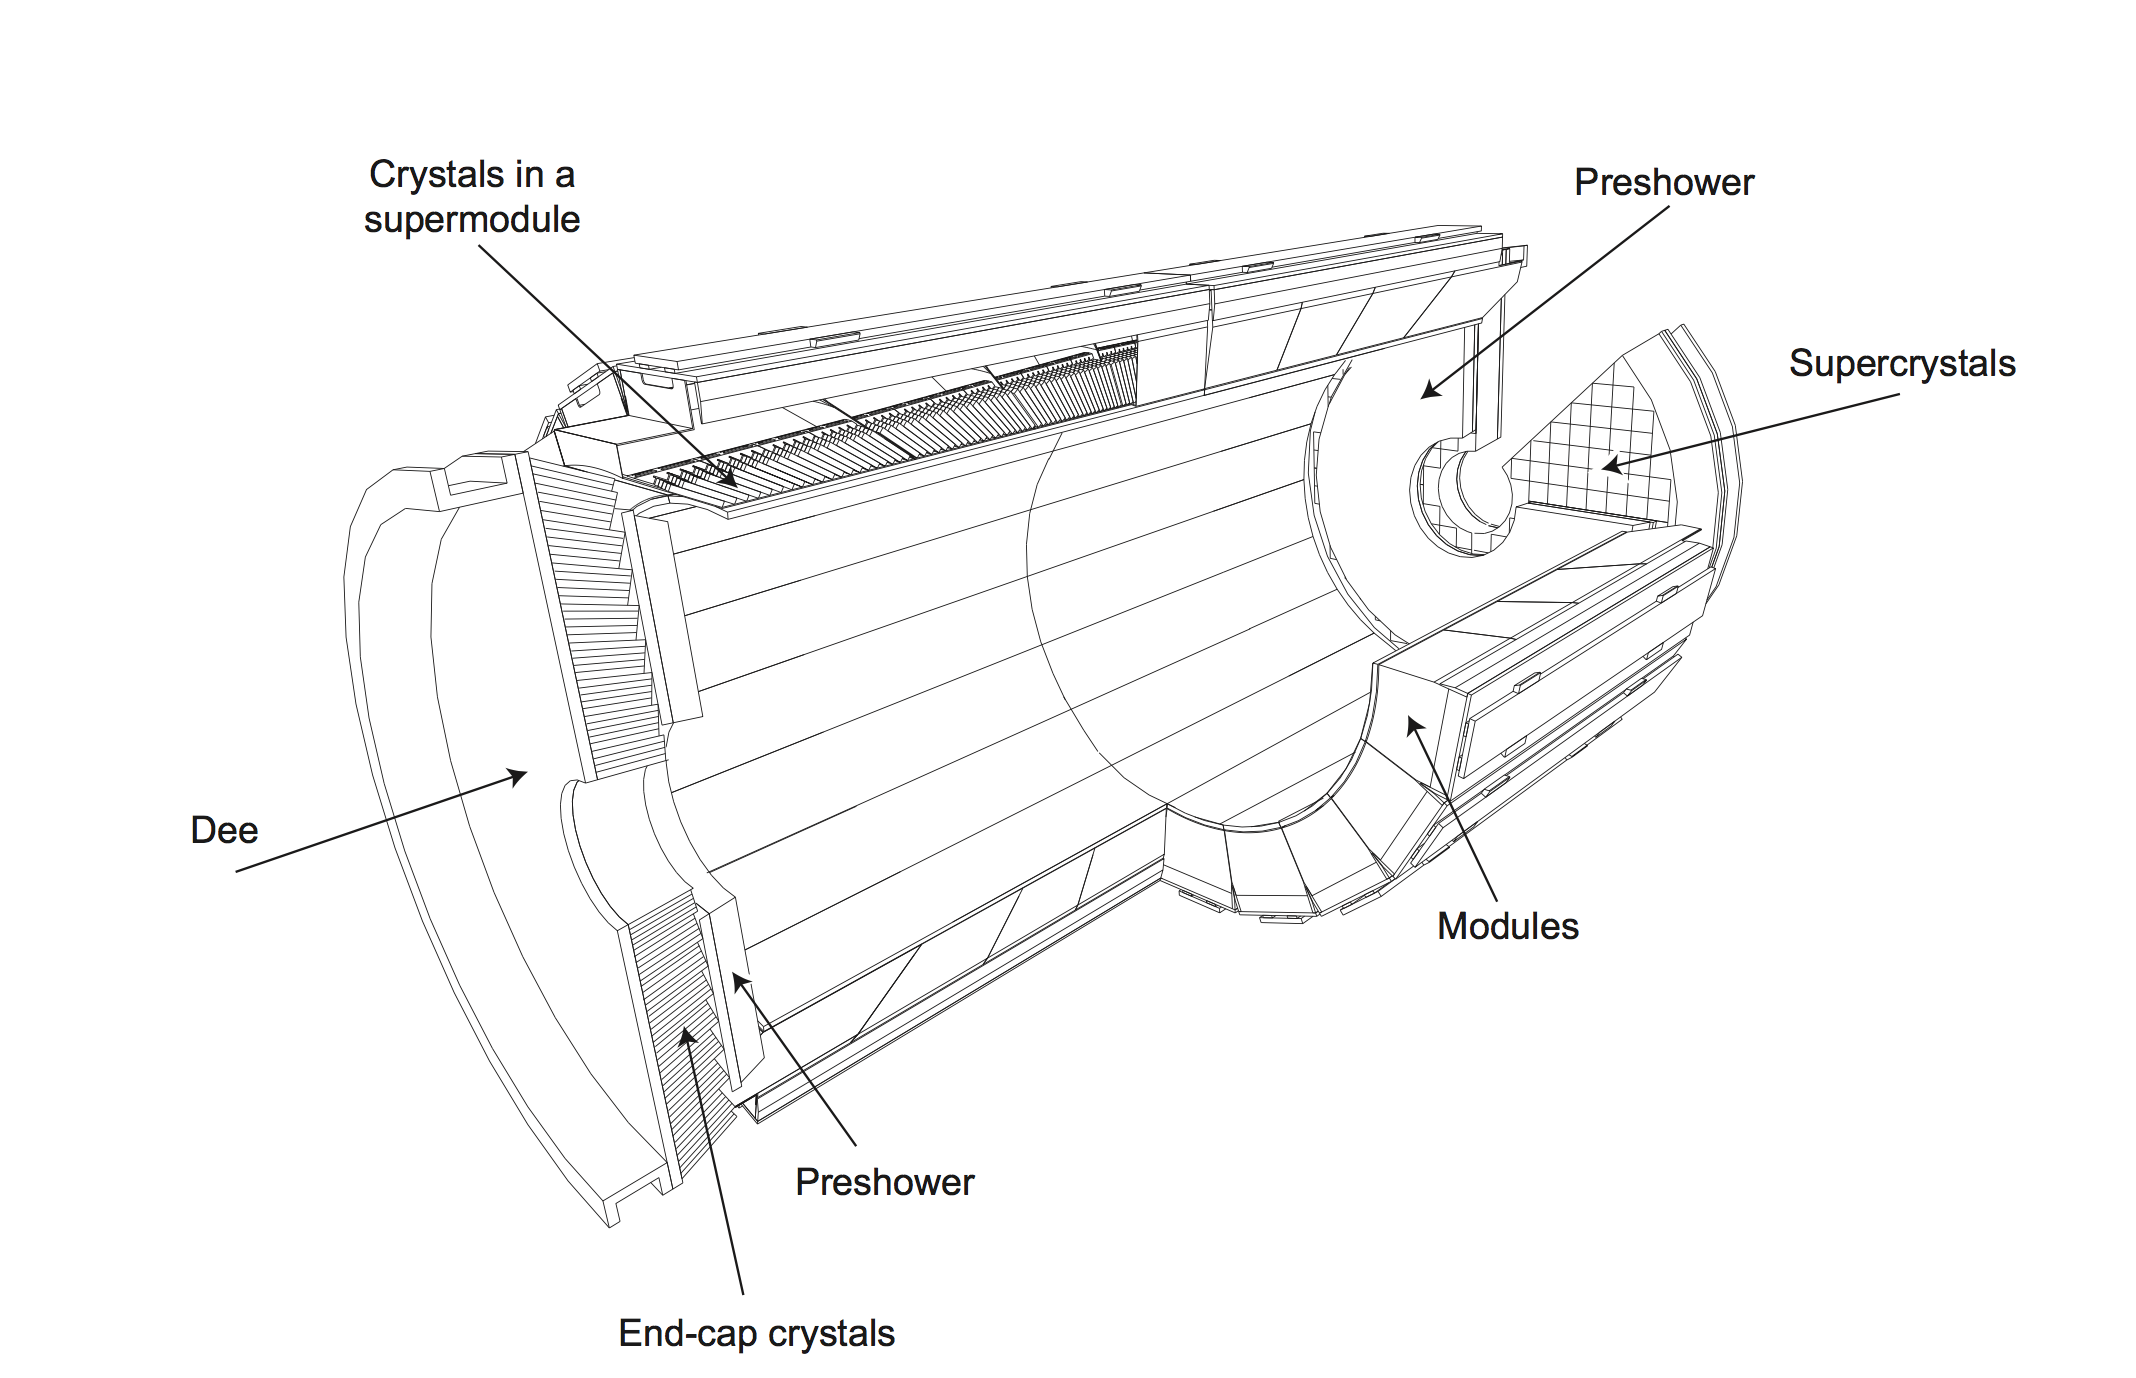
\includegraphics[width=0.9\textwidth]{./Detector/Plots/ECAL.png}
\caption{Layout of the \ac{ECAL}, indicating the position of the
different components \cite{cms-jinst}.}
\label{fig:CMS_ECAL}
\end{center}
\end{figure}

To preserve the energy resolution, the \ac{ECAL} crystal and
photodetector temperatures need to be kept stable within $\pm 0.05^o$C
as the number of scintillation photons emitted by the crystals,
and the amplification of the photodetectors are temperature dependent.
The nominal operating temperature, $18^o$C, is ensured by 
supplying the detector with water at this temperature.

To record the light yield of the crystals, amplifying photodetectors
need to be used. In the \ac{EB} avalance photodiodes are employed
for this, with vacuum phototriodes used in the \ac{EE}.

The energy resolution of the \ac{ECAL} can be parameterised as

\begin{equation}\label{eqn:ecalres}
\frac{\sigma}{E} = \frac{S}{\sqrt{E}}\bigoplus\frac{N}{E}\bigoplusC},
\end{equation}

where $S$ is the stochastic term, $N$ the noise term and $C$ the constant term.
The stochastic term arises from fluctuations in lateral shower containment and 
fluctuations in scintillation, the noise term due to noise from the electronics
and additional particles in the event, and the constant term comes
from calibration errors, and non-uniformity of longitudinal response.

The values of $S$, $N$ and $C$ have been measured in an electron
test-beam, without a magnetic field or material in front of the \ac{ECAL}. These
amounted to $S = 0.028$ GeV$^{\frac{1}{2}}$, $N = 0.12$ GeV, $C= 0.003$.
%S = 2.83 %pm 0.03%, C = 0.26% pm 0.04%



\subsection{\acl{HCAL}}
\label{sec:CMSLHC_CMS_hcal}
The \ac{ECAL} is surrounded by the \ac{HCAL}, important for the
measurement of the energies of strongly interacting particles. As
the \ac{ECAL} extends out to a radius of 1.77 m and the magnet coil
starting at a radius of 2.95 m the barrel region of the \ac{HCAL} consists
of the \ac{HB}, which sits inside the magnet coil, and the \ac{HO}, sitting outside it, 
to complement the \ac{HB}. The \ac{HB} and \ac{HO}  provide coverage up to $|\eta|<1.3$, 
beyond which they are complemented by the \ac{HE} and the \ac{HF}. The \ac{HE} provides
coverage between $1.3<|\eta|<3$ with the \ac{HF} extending this coverage up to $|\eta| = 5.2$
The locations of the different subcomponents of the \ac{HCAL} are shown
in figure \ref{fig:CMS_HCAL}.

\begin{figure}[h!]
\begin{center}
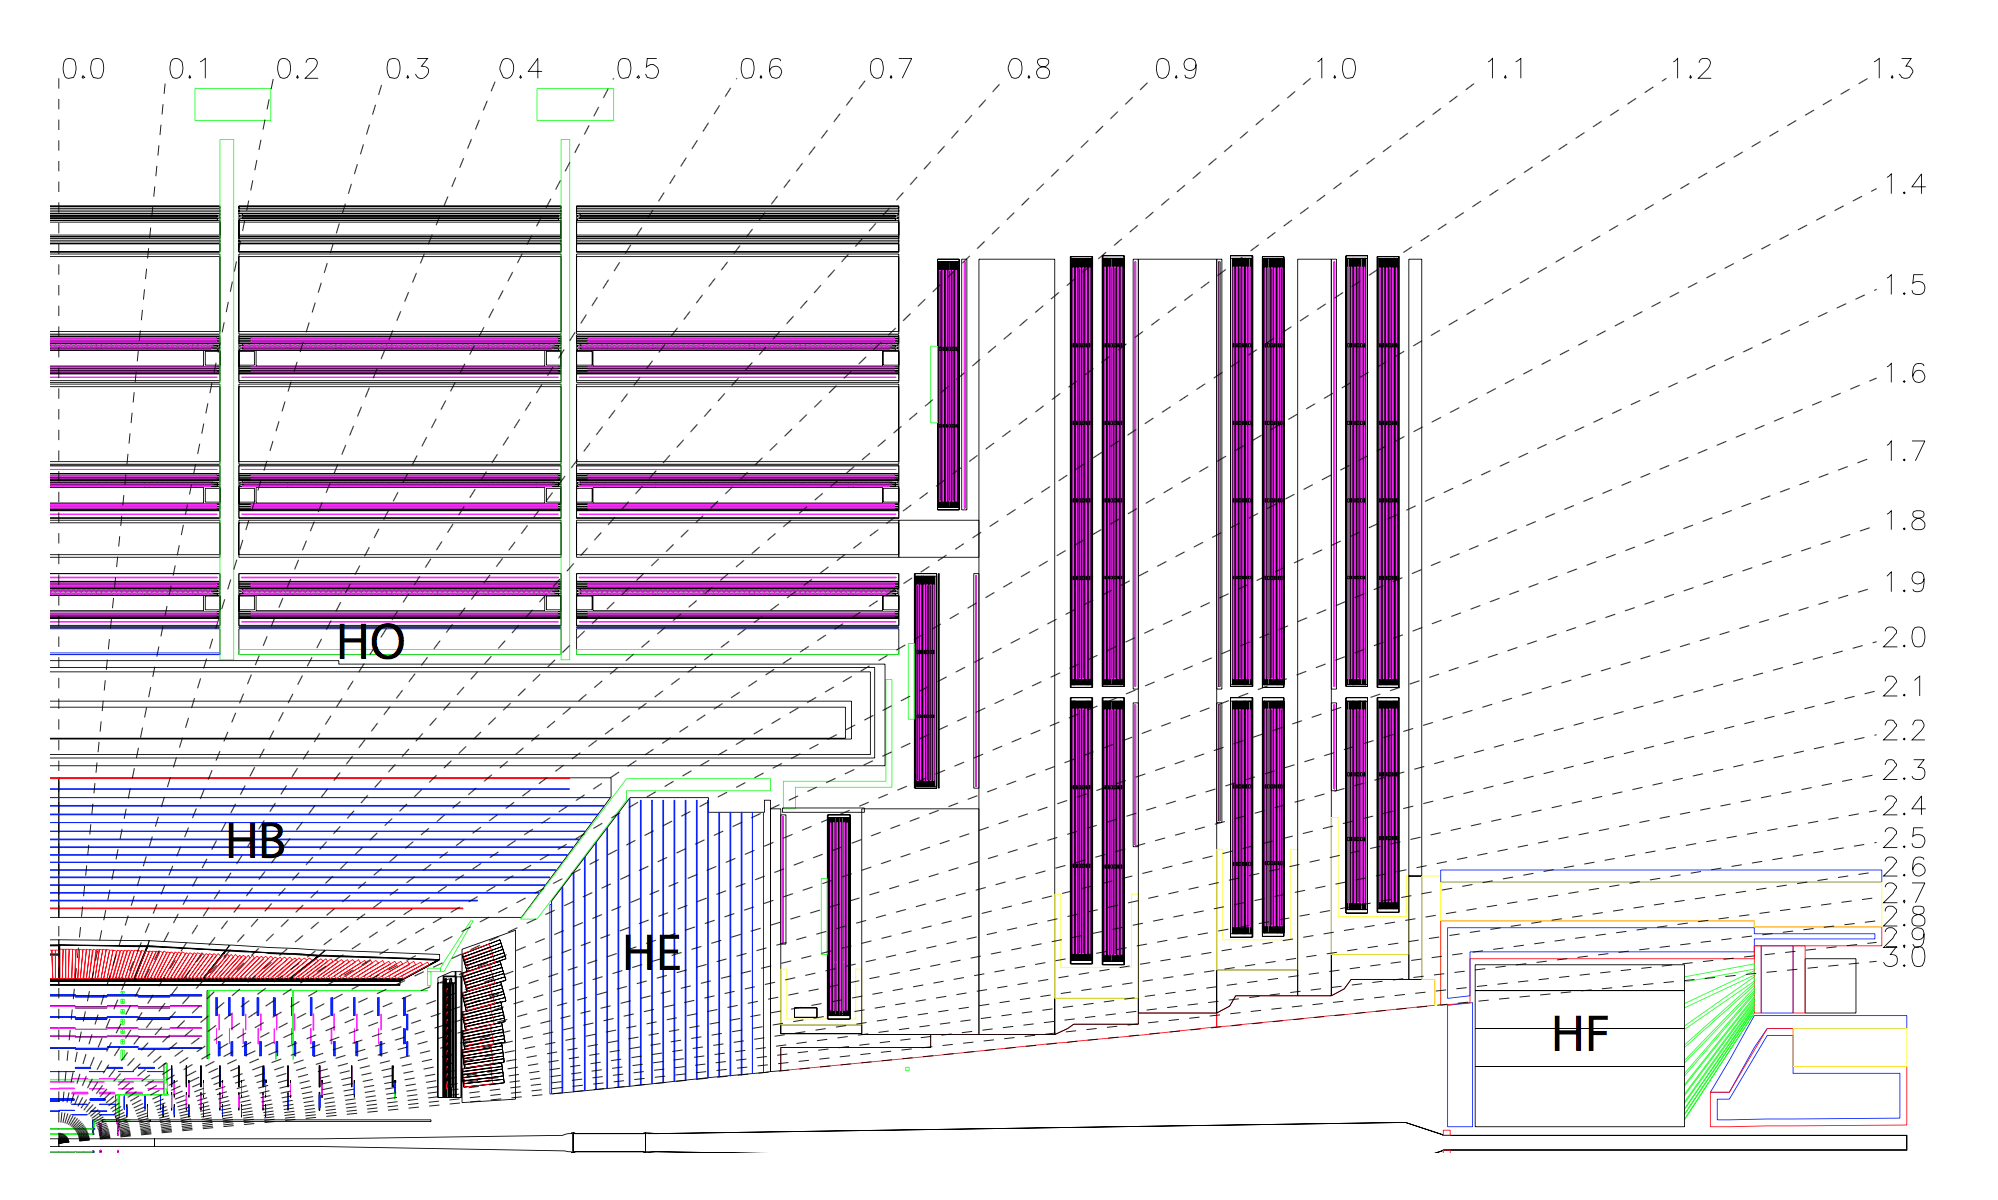
\includegraphics[width=0.9\textwidth]{./Detector/Plots/HCAL.png}
\caption{Illustration of the \ac{HCAL}, indicating the geometry
of the detector \cite{cms-jinst}.}
\label{fig:CMS_HCAL}
\end{center}
\end{figure}

The \ac{HB} and \ac{HE} are sampling calorimeters made of brass absorber
plates with tiles of plastic scintillator as the active material. The tiles 
are $0.087 \times 0.087$ in $\eta-\phi$ for $|\eta|<1.6$ and $0.17\times0.17$ in $\eta-\phi$
beyond this range.
The light from each tile is collected with a wavelength-shifting fibre, 
which is eventually read out using a hybrid photodiode. In the barrel, the \ac{HCAL}
has a thickness of between 5.82 and 10.6 interaction lenghts, which is not 
sufficient to identify for example late-starting showers. The \ac{HO}, sitting
outside of the magnet and using the coil as an additional absorber, extends the 
thickness to at least 11.8 interaction lenghts. 
The active material again consists of plastic scintillator tiles which roughly
map the granularity of the tiles in the \ac{HB}, read out by feeding the light
to a hybrid photodiode via wavelength shifting fibres.
%WTF: wavelength-shifting fibres

The \ac{HF}, providing coverage in the very forward region, is 
subjected to large radiation doses, requiring an extremely
radiation hard active material. For this reason quartz
fibres are used as active material. These fibres are embedded
in the steel absorber structure. Charged particles from the
shower initiated in the steel generate Cherenkov light in 
the quartz fibres, which is read out by photomultiplier tubes.
%Half of the fibres run over the full depth of the absorber
%while the other half starts at a depth of 22 cm, this is
%to distinguish electrons and photons (which deposit a large
%fraction of their energy in the first 22cm) from hadrons.

The energy resolution of the \ac{HCAL} for single charged pions 
was measured in a test beam \cite{cms-hcalecal}
and can be parameterised as 

\begin{equation}\label{eqn:hcal_res}
\frac{\sigma}{E} = \frac{S}{\sqrt{E}} \bigoplus C,
\end{equation}

where $S$ is the stochastic term, found to be 94.3\% %pm 1.2
and $C$ is the constant term, measured to be 8.4\% %pm 1.0
HCAL RESOLUTION!
%UPGRADE
During LS1, the \ac{HO} and \ac{HF} pmts were replaced 



\subsection{Muon system}
\label{sec:CMSLHC_CMS_muons}
One of the main physics goals of the \ac{CMS} experiment
at design was to search for $H\rightarrow ZZ\rightarrow 4\mu$ decays. Muons
suffer less from radiative losses in the tracker material, which means the most accurate
4-body mass can be constructed when using the dimuon final state of the $Z$'s.
Since the discovery of the Higgs boson the ZZ channel has continued to be an important
final state for Higgs measurements, at the same time many \ac{BSM} searches also make use of 
signatures with muons in the final state.
All of this means that good muon identification efficiency and precise muon momentum resolution
are very important. The \ac{CMS} muon system is made up out of three different subsystems which
are all necessary to ensure the identification requirements can be met. It is located
outside of the magnet coil, interspersed in the iron return yoke of the solenoid.
In the barrel of the detector the \ac{DT} chambers provide coverage for $|\eta|<1.2$, with
the \ac{CSC} covering the $0.9<|\eta|<2.4$ region. The \ac{RPCs}, covering the same
regions as both \ac{DT} and \ac{CSCs}, is used as a dedicated triggering system.

A cross-section of one quadrant of the detector, indicating
the positions of the \ac{DT},\ac{CSCs} and \ac{RPCs}, is shown in figure \ref{fig:CMS_MuonSystem}.
The top of the fourth muon endcap station as shown in this figure was added during \ac{LS1}, providing
additional layers of \ac{CSCs} and \ac{RPCs}.
\ac{LS1}.
\begin{figure}[h!]
\begin{center}
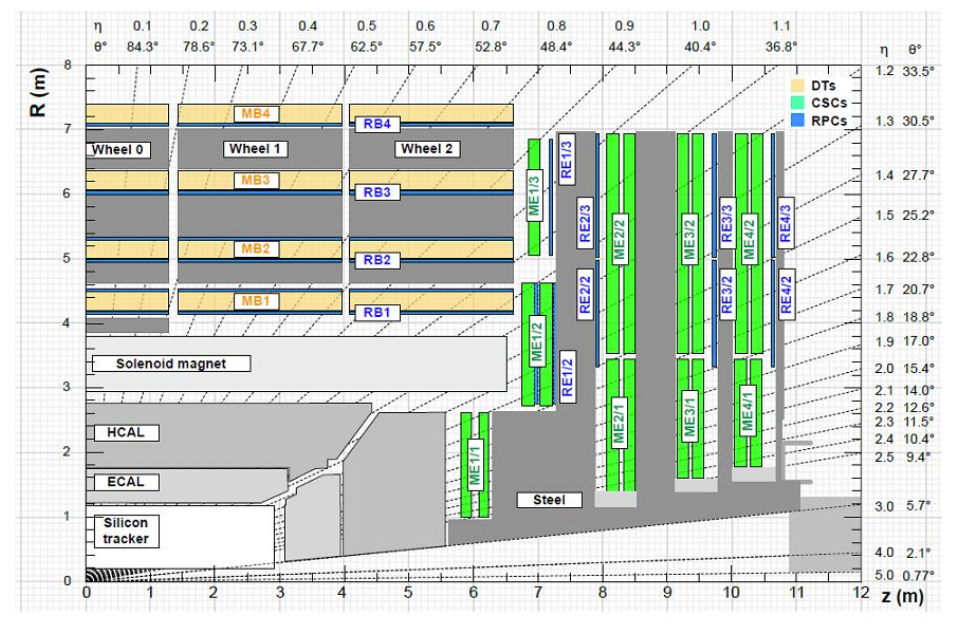
\includegraphics[width=0.8\textwidth]{./Detector/Plots/MuonSystemUpgrade.png}
\caption{Cross-section of one quadrant of the CMS detector, indicating
the positions of the different muon system components \cite{cms-muon-upgrade}. The 
fourth muon endcap stations were extended during \ac{LS1}, in Run 1 only the lower
part existed.}
\label{fig:CMS_MuonSystem}
\end{center}
\end{figure}

The \ac{DT} consists of layers of drift cells with a cross-section of $4.2 \times 1.3$ cm and
2.4 m long. The cells are filled with a mixture of %85\% 
Argon and carbon di-oxide gas.
Muons passing through the chamber ionise the gas, freeing electrons
which drift towards the anode wire running along the centre of the tube-shaped cell. 
This gives rise to an electric signal. There are 4 \ac{DT} stations in each wedge of 
the detector, each in turn consisting of 8 to 12 layers of drift tubes. Some of
these layers are oriented parallel to the beam line, providing a measurement of $\phi$.
There are also layers oriented orthogonal to the beam line, which give a measurement
of the z-coordinate. Measurements of the spatial resolution were made
during proton--proton running of the \ac{LHC} in 2010.
The spatial resolution of the \ac{DT} is 80-120 $\mu$m per chamber for
measurements in the $\phi$ direction, with the resolution of the $z$ measurement
is 130-400 $\mu$m\cite{cms-muon-7tev}.
%Drift lines distorted by magnetic field parallel to the wires

In the endcaps, where the muon rate is higher, the \ac{CSCs} provide
measurements of the muon track. These detectors are radiation-hard,
and have a fast response and fine segmentation.
Each of the CSC modules is a wedge-shaped
multi-wire proportional chamber %WTF
with 6 gaseous chambers bounded by cathode planes, with
sensitive strips placed on these plates in the
radial direction, to measure the coordinate in the  $r-\phi$ plane
of the muons. Anode wires in between the cathode planes
run along the $\phi$ direction and provide a measurement of
$\eta$. The resolution of the $r-\phi$ measurement is 40-120 $\mu$m \cite{cms-muon-7tev}.

In addition to the \ac{DT} and \ac{CSCs}, the \ac{RPCs} provide coverage
for $|\eta|<1.6$. These are made up of parallel plates, forming the anode and cathode,
with a gas gap in between. Ionisation of the gas due to the passing
muons is read out using aluminium strips running parallel to the 
beam axis. The position resolution of the \ac{RPCs} is much poorer than
that of the \ac{DT} and \ac{CSCs}, but their time response is very fast. As
a result of this the \ac{RPCs} can be used as an independent muon trigger
which can correctly identify the beam crossing from which the muon
originated.

To obtain precise muon momentum resolution, information from 
the tracker hits has to be combined with measurements in the
muon stations. The momentum resolution of the muon system
alone is 9\% for muons with \pT up to 200 GeV, and varies with $\eta$ 
between 15-40\% for muons with \pT of 1 TeV.


%Because of the uncertainty in the eventual background rates and in the ability of the muon system to measure the correct beam-crossing time when the LHC reaches full luminosity, a com- plementary, dedicated trigger system consisting of resistive plate chambers (RPC) was added in both the barrel and endcap regions. The RPCs provide a fast, independent, and highly-segmented trigger with a sharp pT threshold over a large portion of the rapidity range (|η| < 1.6) of the muon system. The RPCs are double-gap chambers, operated in avalanche mode to ensure good operation at high rates. They produce a fast response, with good time resolution but coarser position reso- lution than the DTs or CSCs. They also help to resolve ambiguities in attempting to make tracks from multiple hits in a chamber.

\subsection{Triggering and data processing}
\label{sec:CMSLHC_CMS_trigger}
When the \ac{LHC} is operating under standard conditions, protons are collided at a rate
of 40 MHz. This rate is too high for the \ac{DAQ} system to read out every event. In
addition this high collision rate produces such a large number of events that it would
not be feasible to write every single event, with sizes of around 1 MB, to tape. A trigger
system is therefore used to select events of interest for study, which reduces the rate
at which events are written to disk to  $\mathcal{O}(1 \text{ kHz})$.

The trigger system consists of two stages: the \ac{L1} trigger, which only makes use of
front-end electronics 
and reduces the event rate from 40 MHz to around 100 kHz, and the
\ac{HLT}, which runs on a computer farm with around 13000 CPU cores \cite{cms-trigger}.
During \ac{LS1} and the year-end technical stop at the end of 2015 the \ac{L1} trigger was
replaced by a completely upgraded system \cite{cms-trigger-tdr}, which provides amongst others 
improved object isolation, hadronic tau identification, muon \pT resolution and
jet finding with respect to the system used during Run 1.
An overview of the data flow in the \ac{L1} trigger is given in figure \ref{fig:CMS_Trigger}.

\begin{figure}[h!]
\begin{center}
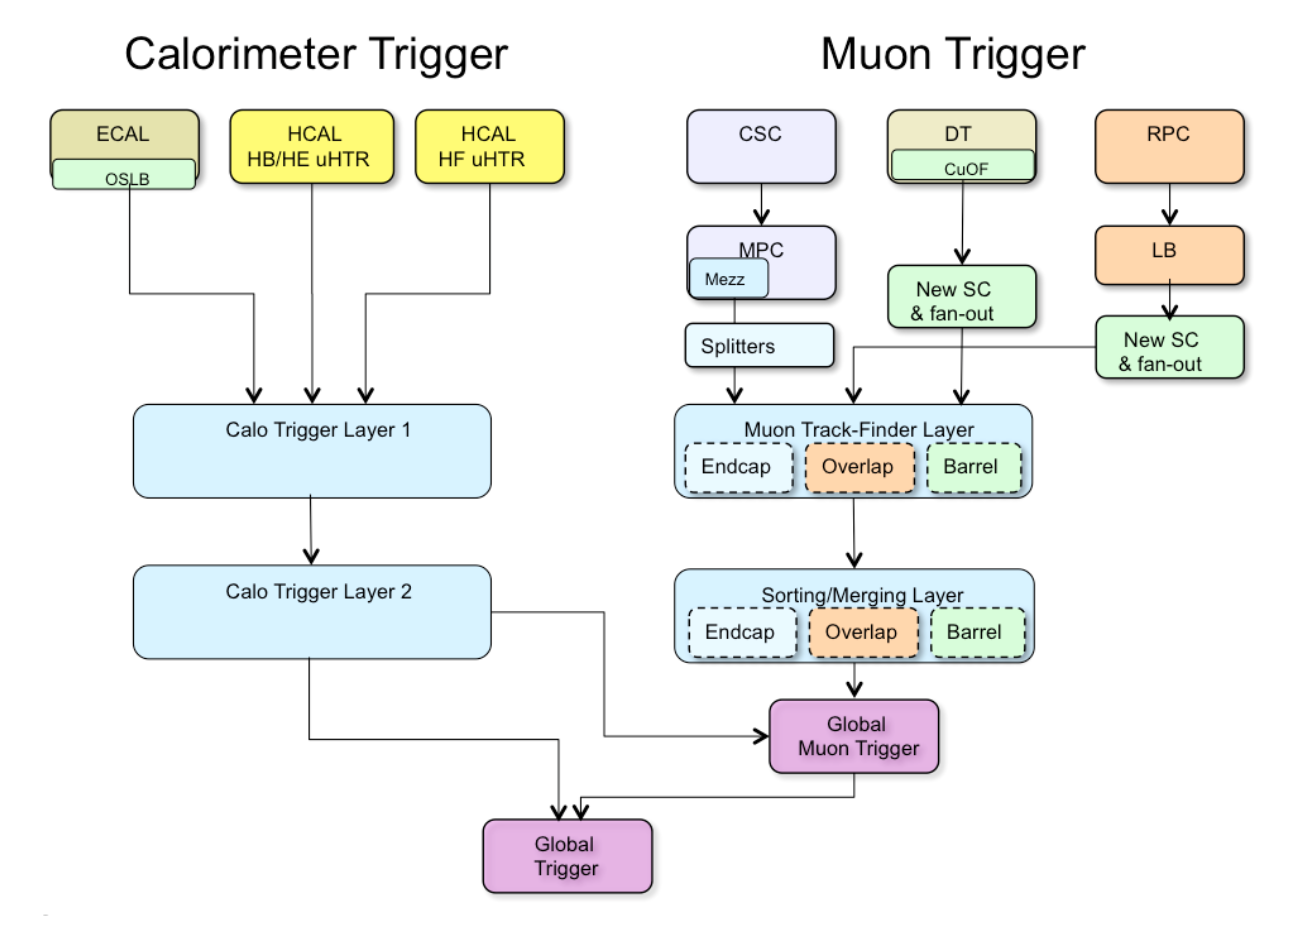
\includegraphics[width=0.5\textwidth]{./Detector/Plots/CMSTrigger.png}
\caption{Schematic of the different components of the \ac{L1} trigger \cite{cms-trigger-tdr}.}
\label{fig:CMS_Trigger}
\end{center}
\end{figure}


The \ac{L1} trigger only makes use of information from the calorimeters and the muon systems.
The calorimeter trigger starts from \ac{HCAL} and \ac{ECAL} energy deposits, 
which are fed to the first layer of the trigger. This layer maps onto
columns of the detector, receiving data from many bunch crossings. These data are passed
on to the second layer of the trigger in a way that bundles data from a single bunch crossing, but
different columns of the detector, to be processed on one node in the second layer of the
trigger. In this step basic object identification is performed based on the energy
deposits, so that a sorted list of the best candidates can be passed to the global trigger.
Hits in the muon chambers are read out and passed to the track finder layer 
of the muon trigger, which combines information from the \ac{CSC}, \ac{DT}
and \ac{RPC} systems in regions of $\eta-\phi$.
In further layers of the muon trigger the information from different
regions is combined, until finally the global muon trigger
can return a sorted list of the best muon candidates to the global trigger.
The global trigger combines the information from the calorimeter and muon triggers
to make a decision on whether the event should be sent to the \ac{HLT} or whether
it should be discarded. A decision has to be made within 3.2 $\mu s$, the maximum time during
which data can be stored in the front-end electronics before being lost.

%The muon trigger is a tracking trigger that measures the momentum of muons using the magnetic field in the steel yoke of the CMS solenoid; thus its resolution degrades with increasing momentum. This can be improved by maximizing the number of chamber hits along a muon trajectory and by improving the precision and number of position and angular measurements participating in the track fit applied in the trigger logic. Moreover, isolation criteria can be applied using the energy deposits in the calorimeter in order to further reduce the rate of muons from heavy flavor jets.

The \ac{HLT}, running on CPU nodes, makes use of the full information
from the detector, including tracker hits. This means particles
can be more accurately identified and their momentum is more
precisely known. The algorithms used in the \ac{HLT} are usually simpler
versions of those used in the full offline reconstruction. %Can't use full because time limited
During the 2012 run of the \ac{LHC} the \ac{HLT} operated with an output
capacity of around 1 kHz, for Run 2 this has increased. In August 2016, 
the \ac{HLT} output rate was 1.2 kHz for immediate data processing, with
an additional 0.6 kHz parked to be reconstructed and analysed when 
more processing power is available\cite{CMS-PAS-HIG-16-037}. %ie at the end of run 2

While the trigger system reduces the rate substantially, several
petabytes of data are produced by \ac{CMS} each year, in addition to 
even larger amounts of simulated datasets. To 
make these large amounts of data easily available for analysis, 
\ac{CMS} and the other \ac{LHC} experiments make use of the \ac{WLCG} \cite{lhc-wlcg}. 
The \ac{WLCG} pools the resources of computer centres at universities and research
laboratories around the world, based on a system of tiers. The Tier 0, at \ac{CERN} and
thw Wigner Research Centre for Physics in Budapest, performs the full reconstruction
and saves the data to tape. Datasets are copied to at least one Tier 1 centre, from
where data can be distributed to Tier 2 centres. The Tier 2 centres are located
at over 150 universities and research institutes around the world, providing 
resources for analysis of the datasets to all researchers associated with the experiment.




  \chapter{Object Reconstruction}
\label{chap:objects}

In this chapter the physics objects necessary to be able to perform searches with \Pgt leptons
in the final state, and how they are reconstructed in \ac{CMS}, will be discussed. The 
descriptions correspond to the algorithms as used during Run 2. Where there are differences
between the algorithms used in Run 1 and Run 2 this will be discussed at the end
of the relevant section.

\section{\acl{PF}}
\label{sec:objects_pf}
All stable particles are reconstructed and identified using the \ac{PF} algorithm, which
combines the information from all of the different subdetectors of \ac{CMS}. This makes
the identification of particles, and determination of position and momentum, as precise
as possible. All of these particles are then used to build for example jets, \MET and hadronically
decaying taus.

The \ac{PF} algorithm starts from charged particle tracks measured
by the inner tracker, muon tracks measured in the muon system, and 
energy deposits in the calorimeters. These energy deposits are combined
using a clustering algorithm, so that stable neutral particles can be identified,
separated from charged hadrons, and electrons and all Bremsstrahlung photons
can be reconstructed. Clustering is performed separately in the \ac{ECAL} barrel,
\ac{ECAL} endcaps, first and second \ac{PS} layers, \ac{HCAL} barrel and \ac{HCAL} endcaps, with no 
clustering employed in the \ac{HF}.
%And to aid energy measurement of charged hadrons for which
%tracks were low quality, or high pT
The clustering algorithm used for \ac{PF} starts from \textit{cluster seeds},
calorimeter cells with local energy maxima. Topological clusters are built by 
merging neighbouring cells into the cluster, provided that the cells
being merged in contain a certain minimum energy.
The threshold is 800 MeV in the \ac{HCAL} and two standard deviations above the
expected noise level in the \ac{ECAL}, meaning 80 MeV in the barrel and up 
to 300 MeV in the endcaps. Cell energies can be shared between multiple
\ac{PF} clusters, depending on the distance between a cell and the centre of the cluster.

Any given particle will usually give rise to multiple \ac{PF}
elements in the different subdetectors. To provide full reconstruction
of each particle, and avoid double counting,  the next step in the
\ac{PF} algorithm is to link the different elements. This is
achieved by defining a distance parameter between any two \ac{PF} elements
in the event, which quantifies the link quality. Directly and indirectly
linked elements are considered as input blocks to the reconstruction and
identification algorithm. Links between charged tracks and calorimeter
clusters are established by extrapolating the track from its last measured
tracker hit to the \ac{PS} layers, the \ac{ECAL} and the \ac{HCAL}. %in ECAL to expected maximum of a 
%typical longitudinal electron shower profile and in the HCAL at a depth correspnding to one interaction
%length.
If the extrapolated track position is within the boundaries of the cluster, plus the size
of one cell in each direction to account for gaps between cells and multiple scattering, the
track is said to be linked to the calorimeter cluster. The distance is taken as the distance $\Delta R$ 
between the position of the cluster and the position of the track. Tangents to tracks are also extrapolated
to the ECAL from the track--tracker layer interaction points, and clusters can be 
linked to the track as a possible Bremsstrahlung photon if the extrapolated tangent
position is within the boundaries of the cluster.
Links between calorimeter clusters are made when the cluster position in the
more granular calorimeter is within the cluster of the less granular calorimeter,
with the link distance again defined as the $\Delta R$ between two cluster positions.
To determine links between charged tracks in the inner tracker and a muon track
in the muon system, a global fit between the two tracks is performed, where the link
is accepted if requirements on the maximum $\chi^2$ of this fit are met. This
$\chi^2$ also determines the distance parameter.

For each block, particles are identified following a sequence
of tests. First, if there is a link between a tracker track and a muon system track,
a particle flow muon is identified if the combined tracker and muon system
momentum is compatible with the tracker-only momentum. %within three standard deviations
The muon track is removed from the block before the next step of the algorithm.

Secondly, tracks are refitted with the \ac{GSF}, the compatibility
of the track with the already linked \ac{ECAL} clusters is assessed using
\ac{BDTs} which take several variables into account. If the candidate
passes, it is identified as a particle flow electron and the track and
\ac{ECAL} clusters are removed from the block.

Following this, remaining tracks lead to charged hadrons. The track is
given the momentum from the track fit, assuming the mass of a charged pion. If
the energy measured in the calorimeters is compatible with the momentum assigned
to the track, within uncertainties, as charged hadron is identified and the
momentum redefined by fitting the tracker and calorimeter measurements. If
the energy of the calorimeter clusters linked to the track is significantly larger than the
charged particle momentum from the track fit, additional overlapping neutral particles
are identified. If the difference between tracker momentum and calorimeter
energies is larger than the total energy registered in associated \ac{ECAL} clusters,
a particle flow photon with energy equal to the total \ac{ECAL} energy is created.
Any remaining momentum difference is assigned to a particle flow neutral hadron. If the momentum
difference is smaller than the energy registered in associated \ac{ECAL} clusters 
only a particle flow photon is created. %Justified by fact that
%in jets 25% of the energy is carried by photons while neutral hadrons
%leave only 3% of the jet energy in the ECAL. This fraction is reduced by one order of magnitued
%for taus for which decays to final states with neutral hadrons are Cabbibo suppressed to a branching ratio of 
%about a percent.

Finally, any remaining \ac{ECAL} clusters not linked to a track give
rise to particle flow photons, with any \ac{HCAL} clusters
not linked to tracks giving rise to particle flow neutral hadrons.

\section{Tracks and vertices}
\label{sec:objects_pv}

\section{Electrons}
\label{sec:objects_ele}

\section{Muons}
\label{sec:objects_muo}

\section{Jets and b-tagging}
\label{sec:objects_jets}

\subsection{Jet energy corrections}
\label{sec:objects_jets_jec}

\section{Missing energy}
\label{sec:objects_met}

\subsection{Recoil corrections}
\label{sec:objects_met_recoilcorr}

\section{Hadronic taus}
\label{sec:objects_tau}
Taus are unstable particles and they decay before reaching the detector. In 17.4 \% of 
cases they decay to muons and neutrinos, with an additional 17.8 \% decaying to electrons
plus neutrinos. The remaining 64.8 \% decay hadronically. Hadronically decaying
taus are characterised by narrow jets containing either one or three charged
particles ($\pi^{\pm}, K^{\pm}$) and 0,1, or two neutral pions. An overview
of the most common possible decay modes is given in table \ref{tab:hadronic_tau_decays}

\begin{table}[htp]
\begin{center}
\caption{Summary of hadronic tau decay modes, indicating the branching fraction, and intermediate resonances where relevant \cite{pdg-2014}.}
\begin{tabular}{@{}lll@{}}
%\toprule
\textbf{Decay mode} & \textbf{Resonance} &\textbf{Branching fraction [\%]}\\
\midrule
\Ptaupm $\rightarrow$ h$^{\pm}$\Pnut & & 11.5\%\\
\Ptaupm $\rightarrow$ h$^{\pm}$\Ppizero\Pnut& $\rho$(770) & 26.0\% \\
\Ptaupm $\rightarrow$ h$^{\pm}$\Ppizero\Ppizero\Pnut & a$_{1}$(1260) & 9.5\% \\
\Ptaupm $\rightarrow$ h$^{\pm}$h$^{\mp}$h$^{\pm}$\Pnut & a$_{1}$(1260) & 9.8\% \\
\Ptaupm $\rightarrow$ h$^{\pm}$h$^{\mp}$h$^{\pm}$\Ppizero\Pnut & & 4.8\%\\
Other modes with hadrons & & 3.2\% \\
\midrule
Total & & 64.8\% \\
%\bottomrule
\end{tabular}
\label{tab:hadronic_tau_decays}
\end{center}
\end{table}

\subsection{Identification}
\label{sec:objects_tau_id}
Hadronic tau decays are reconstructed using the \texttt{hadrons plus strips} (HPS) algorithm~\cite{cms-tau-run1,cms-tau-2015}, 
which is seeded by jets clustered from \ac{PF} candidates, using the anti-\kT algorithm with a distance parameter $\Delta R = 0.4$. 
As table \ref{tab:hadronic_tau_decays}
shows, 60\% of hadronic tau decays contain at least one \Ppizero in the final state. There is a high
probability that photons from $\Ppizero \rightarrow \Pphoton \Pphoton$ decays convert to
\APelectron \Pelectron pairs in the tracker volume, which are bent in the magnetic field and 
therefore cause showers dispersed in the $\phi$ direction in the \ac{ECAL}. Therefore, to 
reconstruct the energy deposits \Ppizero candidates leave in the ECAL, 
the photon and electron constituents of the jet that seeds the $\tau_{h}$ reconstruction are clustered into strips.
The \Pe or \Pphoton with highest \pT that is not yet included in a strip is used to build a new strip.
The $\eta$ and $\phi$ of this candidate determine the initial position of the strip, the next highest \pT \Pe or \Pphoton  
within an $\eta \times \phi$ window centered on the strip location is added to the strip and the position is 
recomputed as the energy-weighted average of the electron/photon constituents in the strip.
This procedure is repeated until there are no more electrons or photons with \pT $>$ 0.5$~GeV  within the 
strip window. The $\Delta \eta$ and $\Delta \phi$ of the strip are varied based on the \pT or \ET to 
be added to the strip and on the energy the strip already has, as

\begin{equation}\label{eqn:dynamicstrip}
\begin{split}
&\Delta \eta  = f(\pT^{\Pe/\Pphoton}) + f(\pT^{\text{strip}}) \notag \\
&\Delta \phi  = g(\pT^{\Pe/\Pphoton}) + g(\pT^{\text{strip}})\\
\end{split}
\end{equation}

Where $\pT^{\Pe/\Pphoton}$ is the transverse momentum of the candidate to be added to the strip
and $\pT^{\text{strip}}$ is the transverse momentum of the strip before merging a new candidate in.\\
In addition, the strip size is bounded as $0.05 < \Delta\eta < 0.15$, $0.05 < \Delta\phi < 0.3$.

The functions $f(p_{\text{T}})$ and $g(p_{\text{T}})$ are defined as:

\begin{equation}\label{eqn:dynamicstripfg}
\begin{split}
&f(\pT) = 0.2\cdot \pT^{-0.66} \text{ and } \notag \\
&g(\pT) = 0.35\cdot \pT^{-0.71}.\\
\end{split}
\end{equation}

If the $\Sigma \pT$ of the strip is at least 2.5~GeV, it is considered as a \Ppizero candidate.
To reconstruct hadronic taus, charged particles and strips are combined into different signatures which are said to be
compatible with a certain decay mode if the selection listed below is satisfied. 
If a candidate satisfies more than one of the hypotheses, the one that maximises the \pT is retained.\\

The decay modes considered for reconstructing hadronic taus are:\\
\begin{itemize}
\item \textbf{One prong + 0 \Ppizero :} One charged particle, no strips.
\item \textbf{One prong + 1 \Ppizero :} One charged particle + one strip with mass $ 0.3 < m_{\Pgt} < 1.3 \sqrt{\pT/100}$~GeV. For momenta
less than 100 GeV, the upper limit is fixed to 1.3 GeV, and for momenta larger than 1044 GeV the upper limit on $m_{\Pgt}$ is fixed to 4.2 GeV.
\item \textbf{One prong + 2 \Ppizero :} One charged particle + two strips. The $\Pgt$ mass should be $0.4 < m_{\Pgt} < 1.2\sqrt{\pT/100}$~GeV. For momenta
less than 100 GeV, the upper limit is fixed to 1.2 GeV and for momenta larger than 1111 GeV the upper limit on $m_{\Pgt}$ is fixed to 4.0 GeV.
\item \textbf{Three prong + 0 \Ppizero: } Three charged particles with mass $0.8 < m_{\tau} < 1.5$~GeV. The tracks are required to originate 
within $\Delta z<0.4$~cm of the same vertex, and their total charge is required to be $\pm 1$.
\end{itemize}

\subsection{Isolation and discrimination against light leptons}
\label{sec:objects_tau_iso}


\subsection{Differences between Run 1 and Run 2}
\label{sec:objects_taus_diff}
Broadly speaking the algorithm used for hadronic tau reconstruction during Run 1
was similar to the Run 2 algorithm described earlier in this section. However, during
Run 1 strips were reconstructed using a fixed size of $0.05 \times 0.20$ in $\eta \times \phi$.
The dynamic size used in Run 2 was introduced to mitigate the effects of secondary particles
with low \pT and multiple \APelectron\Pelectron conversions, resulting in particles ending up outside of 
the strip window and making the hadronic tau seem less isolated than it actually is.
SOMETHING ABOUT Jet->Tau FAKE RATES AND e->TAU Misidentification




  \chapter{\texorpdfstring{Search for \Htohhtobbtautau}{Search for H -> hh -> bbtautau}}
\label{sec:hhh}
In this chapter the search for a heavy Higgs boson decaying to a pair of 125 GeV Higgs bosons, with one of these Higgs bosons decaying to 
a pair of b-jets and the other decaying to a pair of \Ptau leptons is discussed. In this analysis the \etau, \mutau and \tautau final states
of the \Pgt-pair are studied, these final states are referred to as channels.
The results of this search are model-independent
upper limits on heavy Higgs production cross--section times branching ratio into h(125)h(125)$\rightarrow b\bar{b} \tau\tau$, for
which all three channels are combined. The \etau and \mutau channels will be described in this chapter, the \tautau channel will not
be covered, although the limits shown in section \ref{sec:hhh_results} will include this final state.
In addition  the results are interpreted in the context of the MSSM and a type-II Two Higgs Doublet Model (2HDM), 
these interpretations are made in combination with the results of a search for \AtoZhtolltautau. 
This search will be summarised in this chapter, but will not constitute the main focus.
Both searches, and their interpretation, are detailed in reference \cite{CMS-HIG-14-034}.

The discovery of the 125 GeV Higgs boson by the ATLAS and CMS collaborations in 2012 \cite{HDiscoveryAtlas,HDiscoveryCMS} has opened up
new possibilities for probing the Higgs sector beyond the Standard Model. As discussed in chapter THEORY, in some MSSM scenarios, and some more
generic type-II 2HDM's, a heavy neutral Higgs boson H can decay to a pair of 125 GeV Higgs bosons for low values
of \tanb, probing a region of phase space not yet excluded by stringent existing limits. In regions where
the decay \Htohh is enhanced, the \AtoZh decay also has a large branching ratio, indicating the usefulness
of both channels for probing the low-\tanb region. The $b\bar{b}$\tautau final state is chosen for the combination
of the large $h(125) \rightarrow b\bar{b}$ branching ratio and the cleaner \htotautau final state.

\section{Datasets and \acl{MC} samples}
\label{sec:hhh_datasets}
The dataset used for this analysis corresponds to the full dataset collected by the CMS experiment during the 2012 $p-p$ 
running period of the LHC. 
Signal and background events were generated using several different \ac{MC} event generators. The \texttt{MadGraph}
\cite{madgraph} matrix element generator was used to generate samples of \Wjets, \Zellell, \ttbar and \ZZ ,\WZ and \WW
events. In addition to samples with a mixture of jet multiplicities (`inclusive' samples), samples binned in jet multiplicity
were used for the \Wjets and \Zellell backgrounds. This increases the background event statistics
in regions with multiple jets, which important for this analysis due to the presence of b-jets in the searched-for final state. 
The samples binned in jet multiplicity are combined with the
inclusive samples such that the fraction of events with each jet multiplicity is preserved.

Single top samples were produced with the \texttt{POWHEG} \cite{powheg1,powheg2} generator. Samples of $gg\rightarrow$\Htohhtobbtautau
were generated in steps of 10 GeV between \mH $= 260 - 350$~GeV using \texttt{PYTHIA 6} \cite{pythia64}. In all of the samples
\texttt{TAUOLA} \cite{tauola} is used to decay $\tau$s, and parton showering and hadronisation are modelled using \texttt{PYTHIA 6} \cite{pythia64}.
Minimum bias events generated using \texttt{PYTHIA 6} are added to all \ac{MC} samples to model additional
interactions. 

To better model the \Ztautau background, an embedding technique is used. In this method, 
\Zmm events are selected in data and the muons are replaced by generator-level taus. \texttt{TAUOLA} is used
to decay the taus and tau polarisation effectes are modelled using \texttt{TauSpinner} \cite{TauSpinner}. The detector
response to the tau decay products is modelled using the \texttt{GEANT4}-based \cite{Geant4} detector simulation, and 
tracks in the inner tracking system, hits in the muon systems and energy deposits in the calorimeters
due to the simulated taus are combined with the remains of the \Zmm event after the detector signals
of the two muons originiating from the \PZ have been removed. This technique is also applied to 
a \ttbar background sample to estimate the \ttbar contamination in the embedded sample. This contribution
needs to be subtracted from the \Ztautau background estimated using the embedded \Zmm sample to
avoid double counting with the \ttbar \ac{MC}.

\section{Event selection and categorisation}
\label{sec:hhh_selection}
A more detailed description of the physics objects used for this analysis is given in chapter OBJECTS
in this section only an overview of the event selection is presented.

\subsection{\texorpdfstring{Event selection in the \mutau channel}{Event selection in the mu-tau channel}}
\label{sec:hhh_selection_mutau}
The first step of event selection in the \mutau channel is a trigger 
which requires only a muon
at L1. At the level of the HLT a hadronic tau, reconstructed using a simpler version of the
PF algorithm, is also required. Loose isolation requirements are applied to this hadronic tau, and 
loose ID and isolation requirements are applied to the muon at this stage.

In the offline event selection, an oppositely charged \mutau pair is required, 
separated by $\Delta R > 0.5$.
The muon is required to have a \pT~of at 
least 20 GeV and $|\eta| < 2.1$, and should be compatible with originating from the 
primary vertex. This means the impact parameters $d_{xy}$ and $d_{z}$ must be smaller
than 0.045 and 0.2 cm respectively. Tight muon identification
criteria and tight isolation requirements $I_{\text{rel}}^{\mu} < 0.1$, as described 
in section OBJECTS, are applied. The hadronic tau must have a \pT~of at least
20 GeV, $|\eta| < 2.3$, and must have $d_{z} < 0.2$ cm. It is required to pass 
the decay mode finding identification
from the HPS algorithm, as described in section OBJECTS. Additionally
the raw combined isolation, described in the same section, is required to be
at most 1.5 GeV. To reject $\Pe/\Pgm \rightarrow \Pgt_{h}$ fakes, and to
reduce the contribution of \Zmm background events, the hadronic tau is 
also required to pass the tight working point of the anti-$\Pgm$ discriminator
and the loose working point of the cut--based anti-$\Pe$ discriminator, both
described in section OBJECTS.

After this selection there is still a chance more than one possible 
\mutau pair exists
in the event. If this is the case, the combination with largest 
\pT$^{\Pgm}$ + \pT$^{\Pgt_{h}}$ is chosen. In order to reduce \Zmm 
backgrounds further, for cases where the reconstructed hadronic tau originates
from a misidentified jet, the event is rejected if an opposite--charge pair 
of lower \pT (at least 15 GeV) muons, passing looser ID and isolation requirements
than the signal muon, can be formed. Additional vetos, requiring exactly one muon and 
exactly zero electrons to pass \pT $>10$ GeV and loose ID and isolation requirements, 
are applied to reduce the \WZ background. 

In addition to the requirements on the di--tau pair, at least 2 jets with \pT$ >20$ GeV are 
required. No b--tagging requirements are applied at this stage, these will be discussed 
in more detail in section \ref{sec:hhh_selection_categories}.

%Figure \ref{fig:Hhh_selection_kinematics_mt} shows some of the kinematic variables 
%of di-\Pgt candidates in the \mutau channel
%\begin{figure}[h!]
%\begin{center}
% \subfloat[Muon \pT]{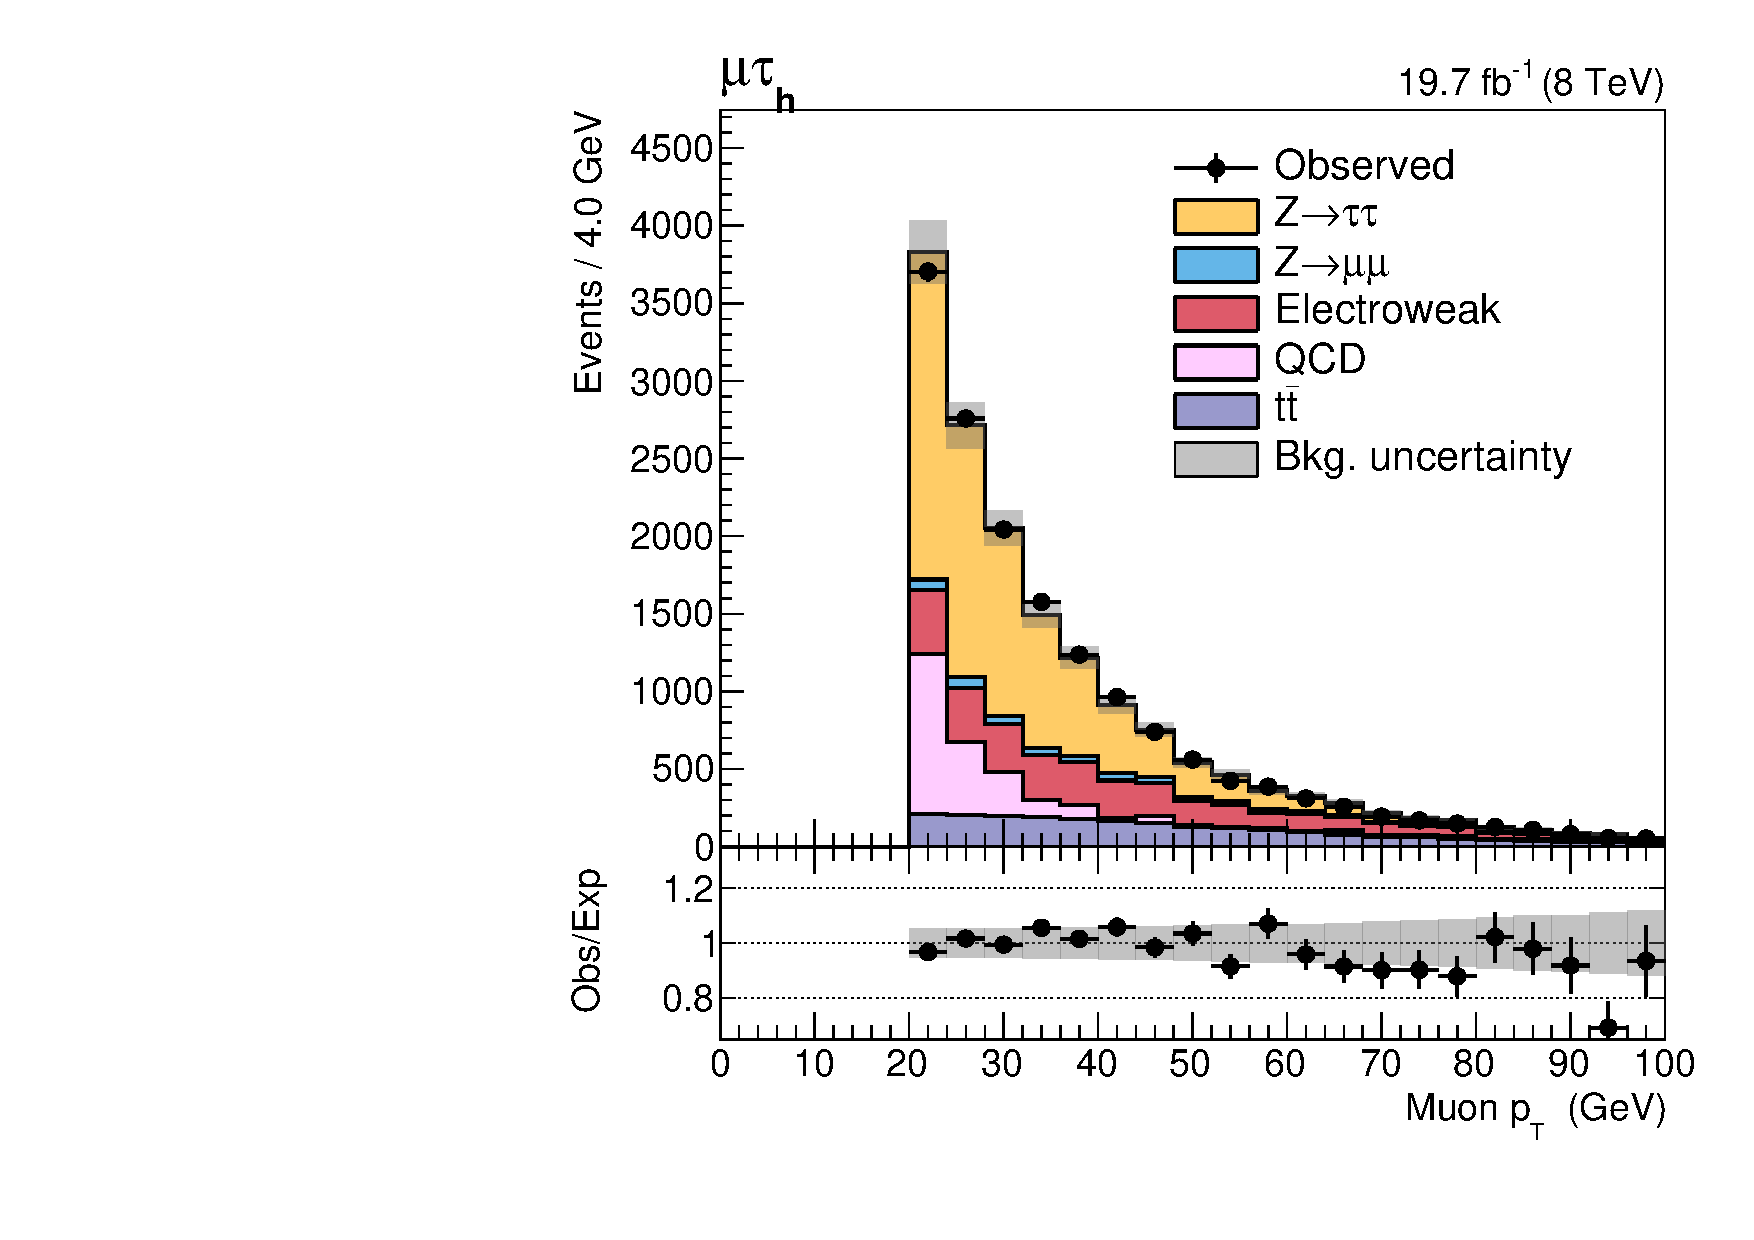
\includegraphics[width=0.5\textwidth]{Hhh/Plots/pt_1_2jetinclusive_mt_2012.pdf}}
%  \subfloat[Hadronic \Pgt \pT ]{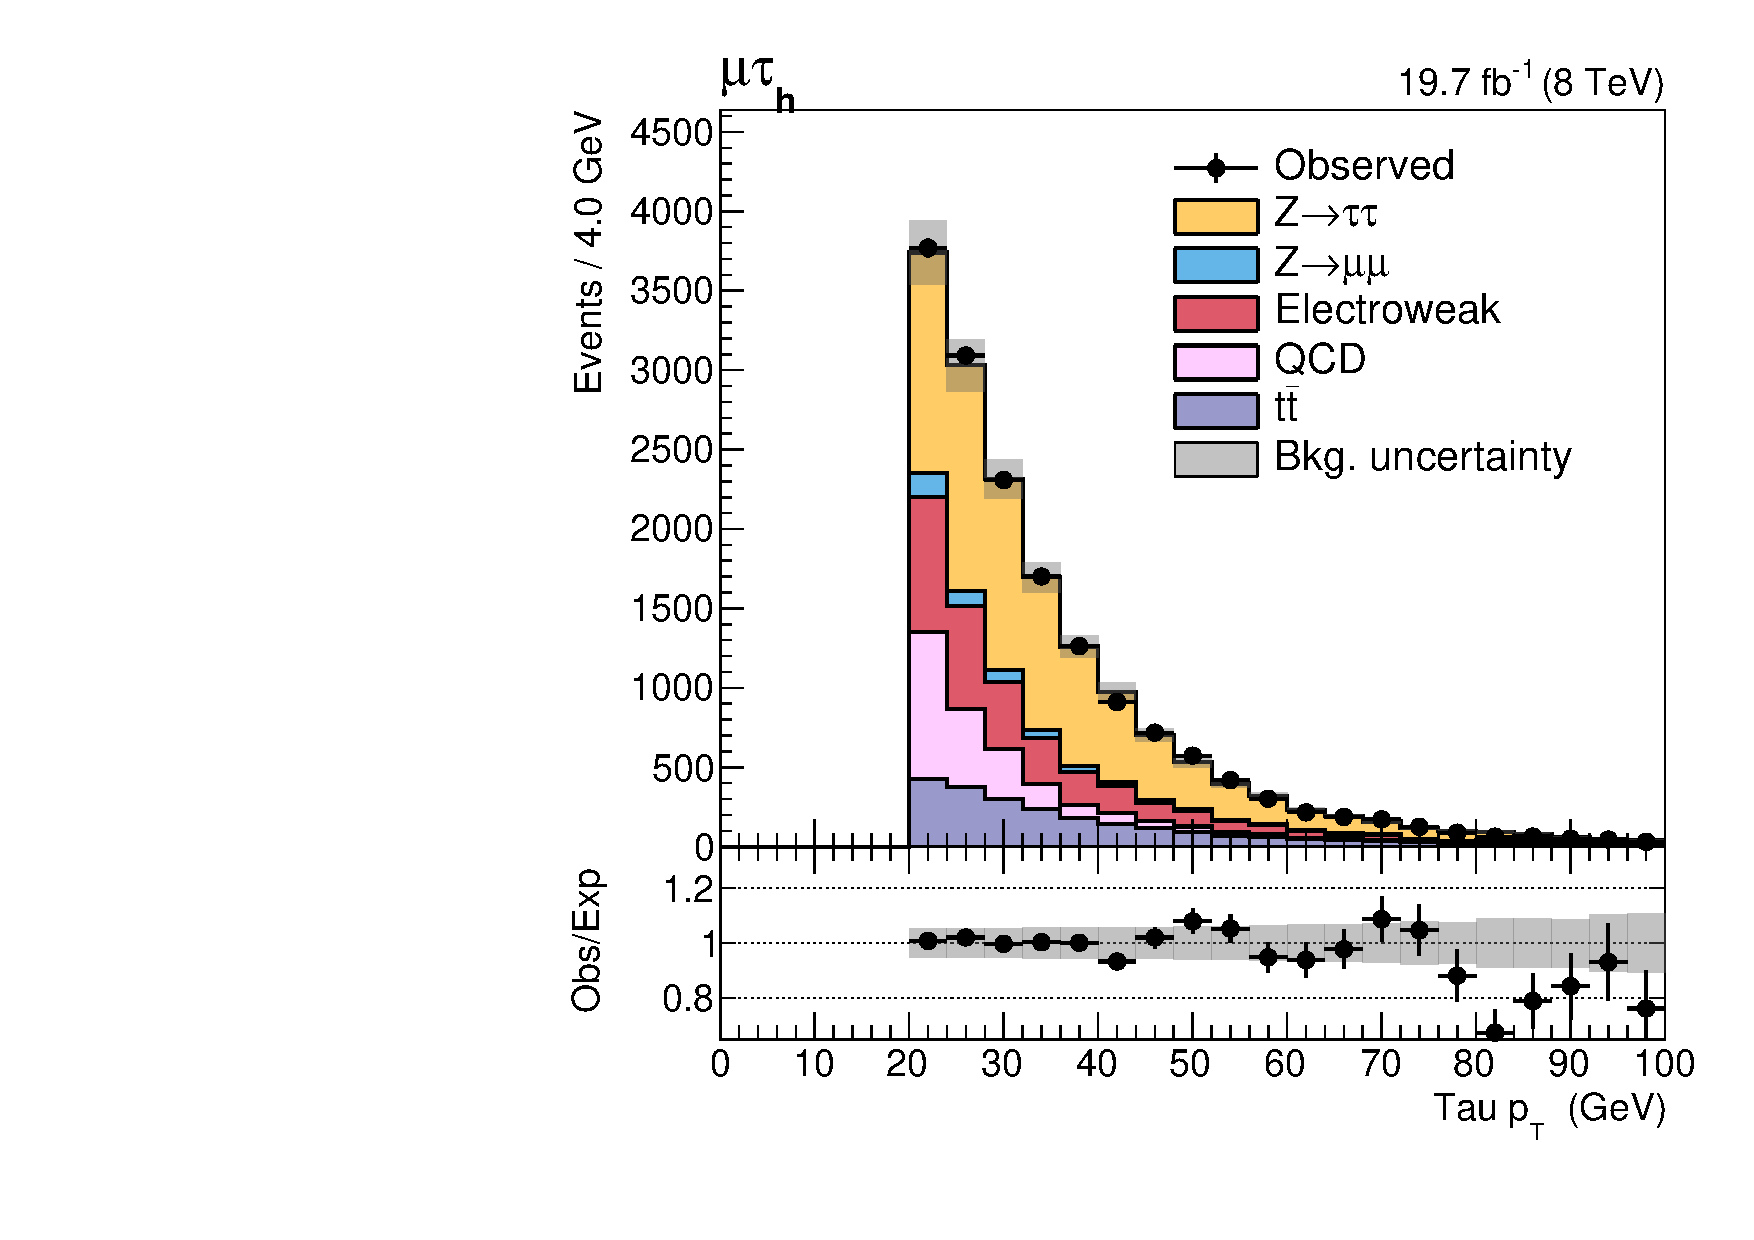
\includegraphics[width=0.5\textwidth]{Hhh/Plots/pt_2_2jetinclusive_mt_2012.pdf}}~\\
%  \subfloat[Muon $\eta$]{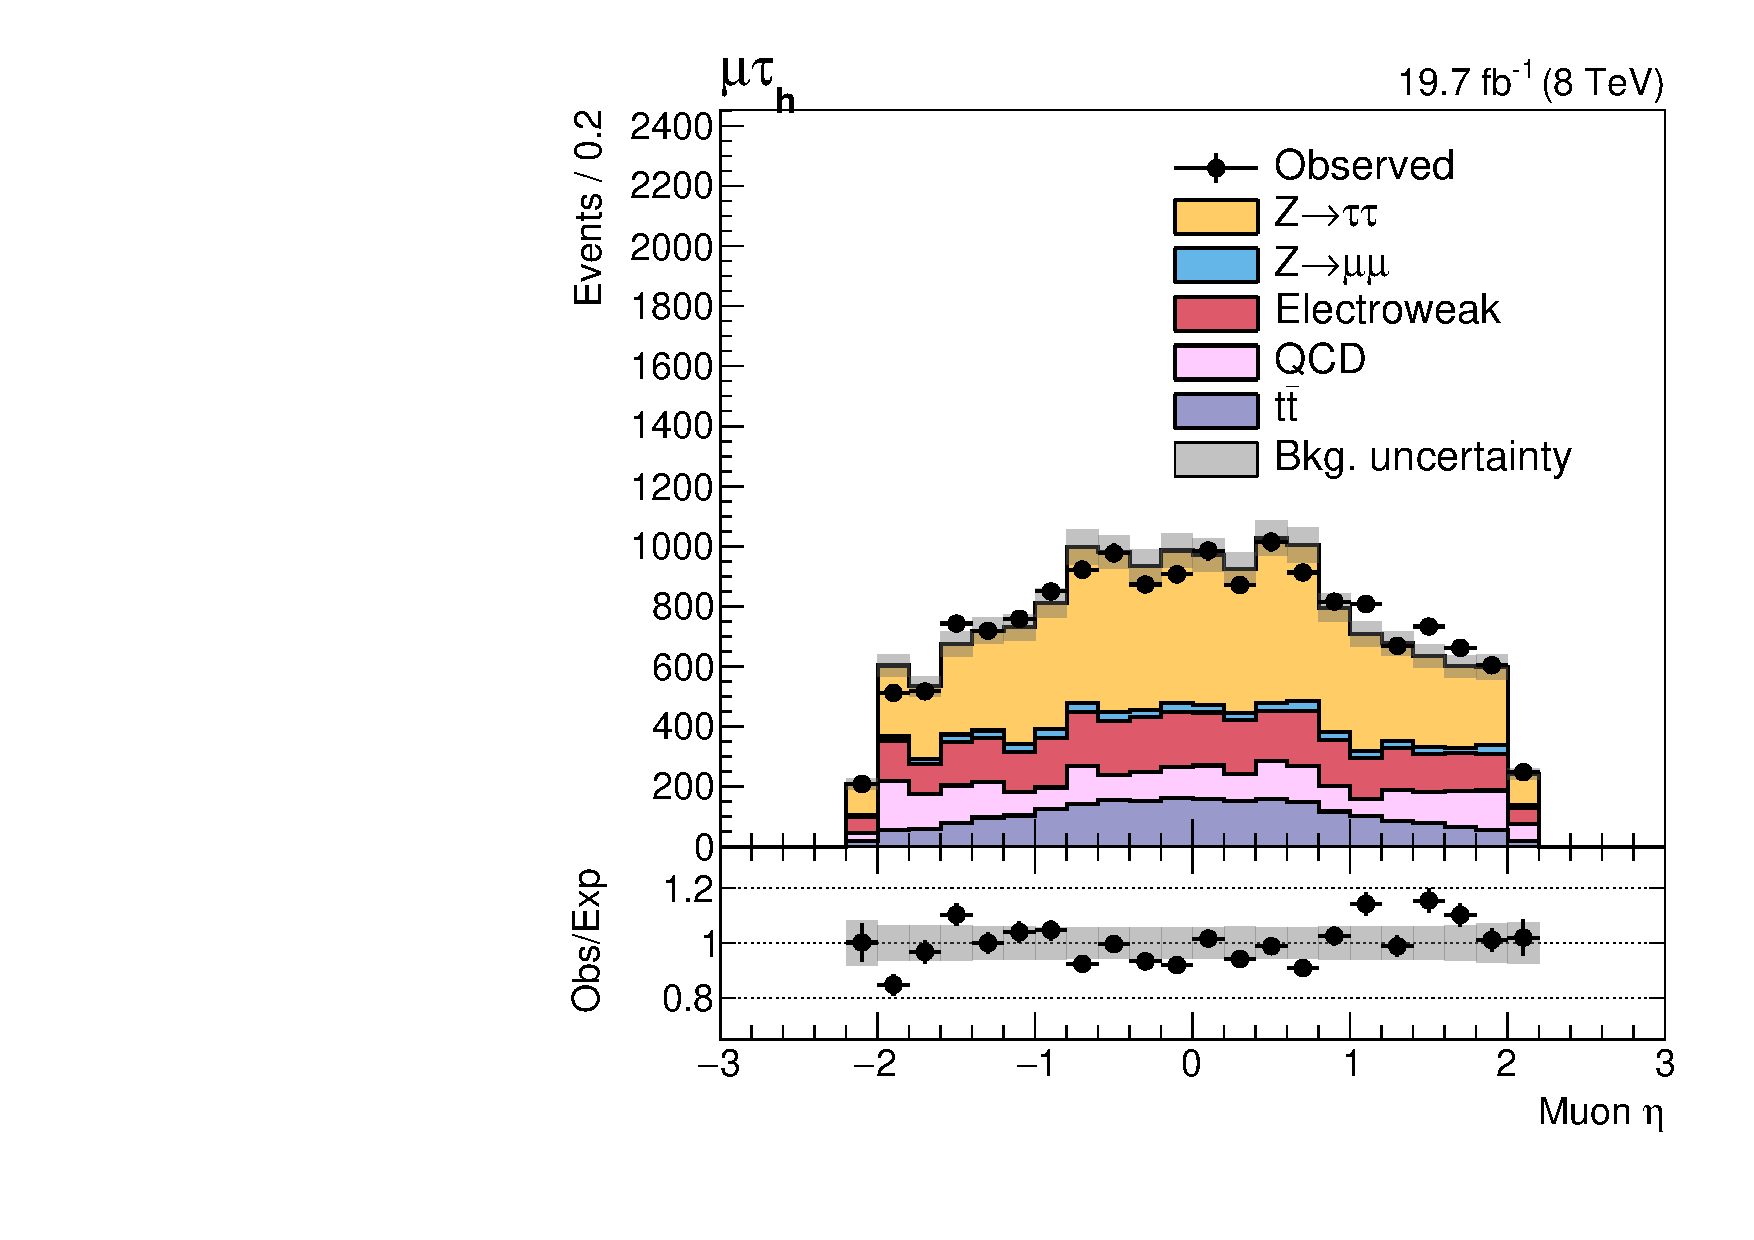
\includegraphics[width=0.5\textwidth]{Hhh/Plots/eta_1_2jetinclusive_mt_2012.pdf}}
%  \subfloat[Hadronic \Pgt $\eta$ ]{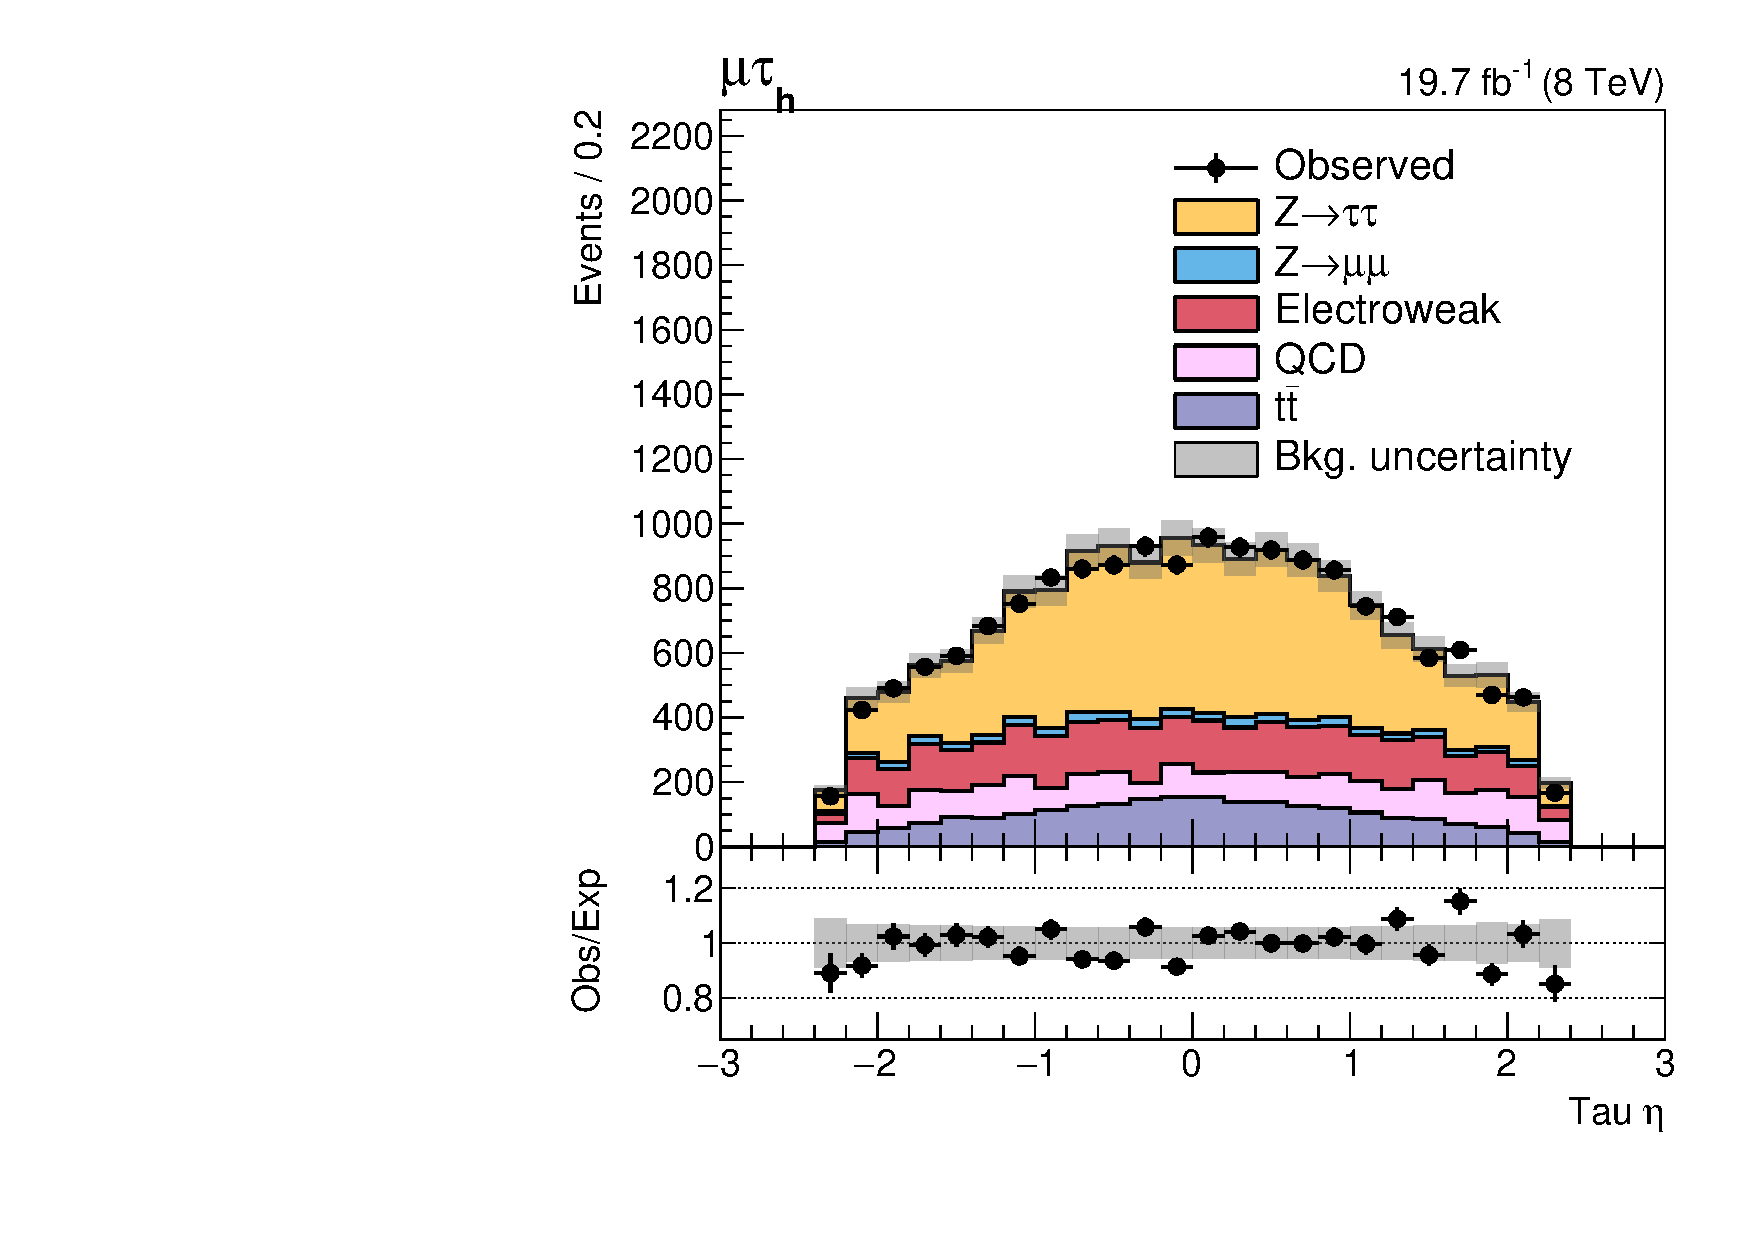
\includegraphics[width=0.5\textwidth]{Hhh/Plots/eta_2_2jetinclusive_mt_2012.pdf}}~\\
%
%\end{center}
%\caption{Plots of muon and hadronic \Pgt \pT and $\eta$ in the \mutau channel.}
%\label{fig:Hhh_selection_kinematics_mt}
%\end{figure}


\subsection{\texorpdfstring{Event selection in the \etau channel}{Event selection in the e-tau channel}}
\label{sec:hhh_selection_etau}
Events in the \etau channel are selected using a trigger which requires an electron at L1, and both an electron
and a hadronic tau at HLT.
The hadronic
tau is reconstructed in a similar way as for the trigger in the \mutau channel, and loose ID and isolation requirements
are also applied to the electron at this stage.

After the trigger selection, an oppositely charged \etau pair is required, again separated by $\Delta R >0.5$. 
The electron should have a \pT~of at least 24 GeV, $|\eta| < 2.1$, and should
satisfy $d_{xy} < 0.045$cm and $d_{z} < 0.2$ cm. The electron must pass the tight
working point of the electron MVA ID discriminator described in section OBJECTS, and the
relative isolation is required to be $I_{rel}^{\Pe} < 0.1$. The requirements placed on the
hadronic tau are similar to those required in the \mutau channel, apart from the anti-$\Pgm$ discriminator,
where the loose working point is required, and the anti--$\Pe$ discriminator, where the medium
working point of the MVA discriminator is required.

If there is more than one possible \etau pair, the pair with largest \pT$^{\Pe}$+\pT$^{\Pgt_{h}}$
is taken. Similar additional vetos as in the \mutau channel are applied.
the event is rejected if an opposite--charge pair of electrons with \pT $> 15$ GeV, passing looser ID and
isolation requirements than the signal electron requirements can be formed. To reduce the \WZ
background, events that have more than one electron or at least one muon passing \pT $>10$ GeV and loose ID and isolation
requirements are rejected.

In addition to the requirements on the di--tau pair, at least 2 jets with \pT $>20$ GeV are 
required. 

%Figure \ref{fig:Hhh_selection_kinematics_etmt} shows some of the kinematic variables 
%of di-\Pgt candidates in the \etau and \mutau channels
%\begin{figure}[h!]
%\begin{center}
% \subfloat[Electron \pT (\etau)]{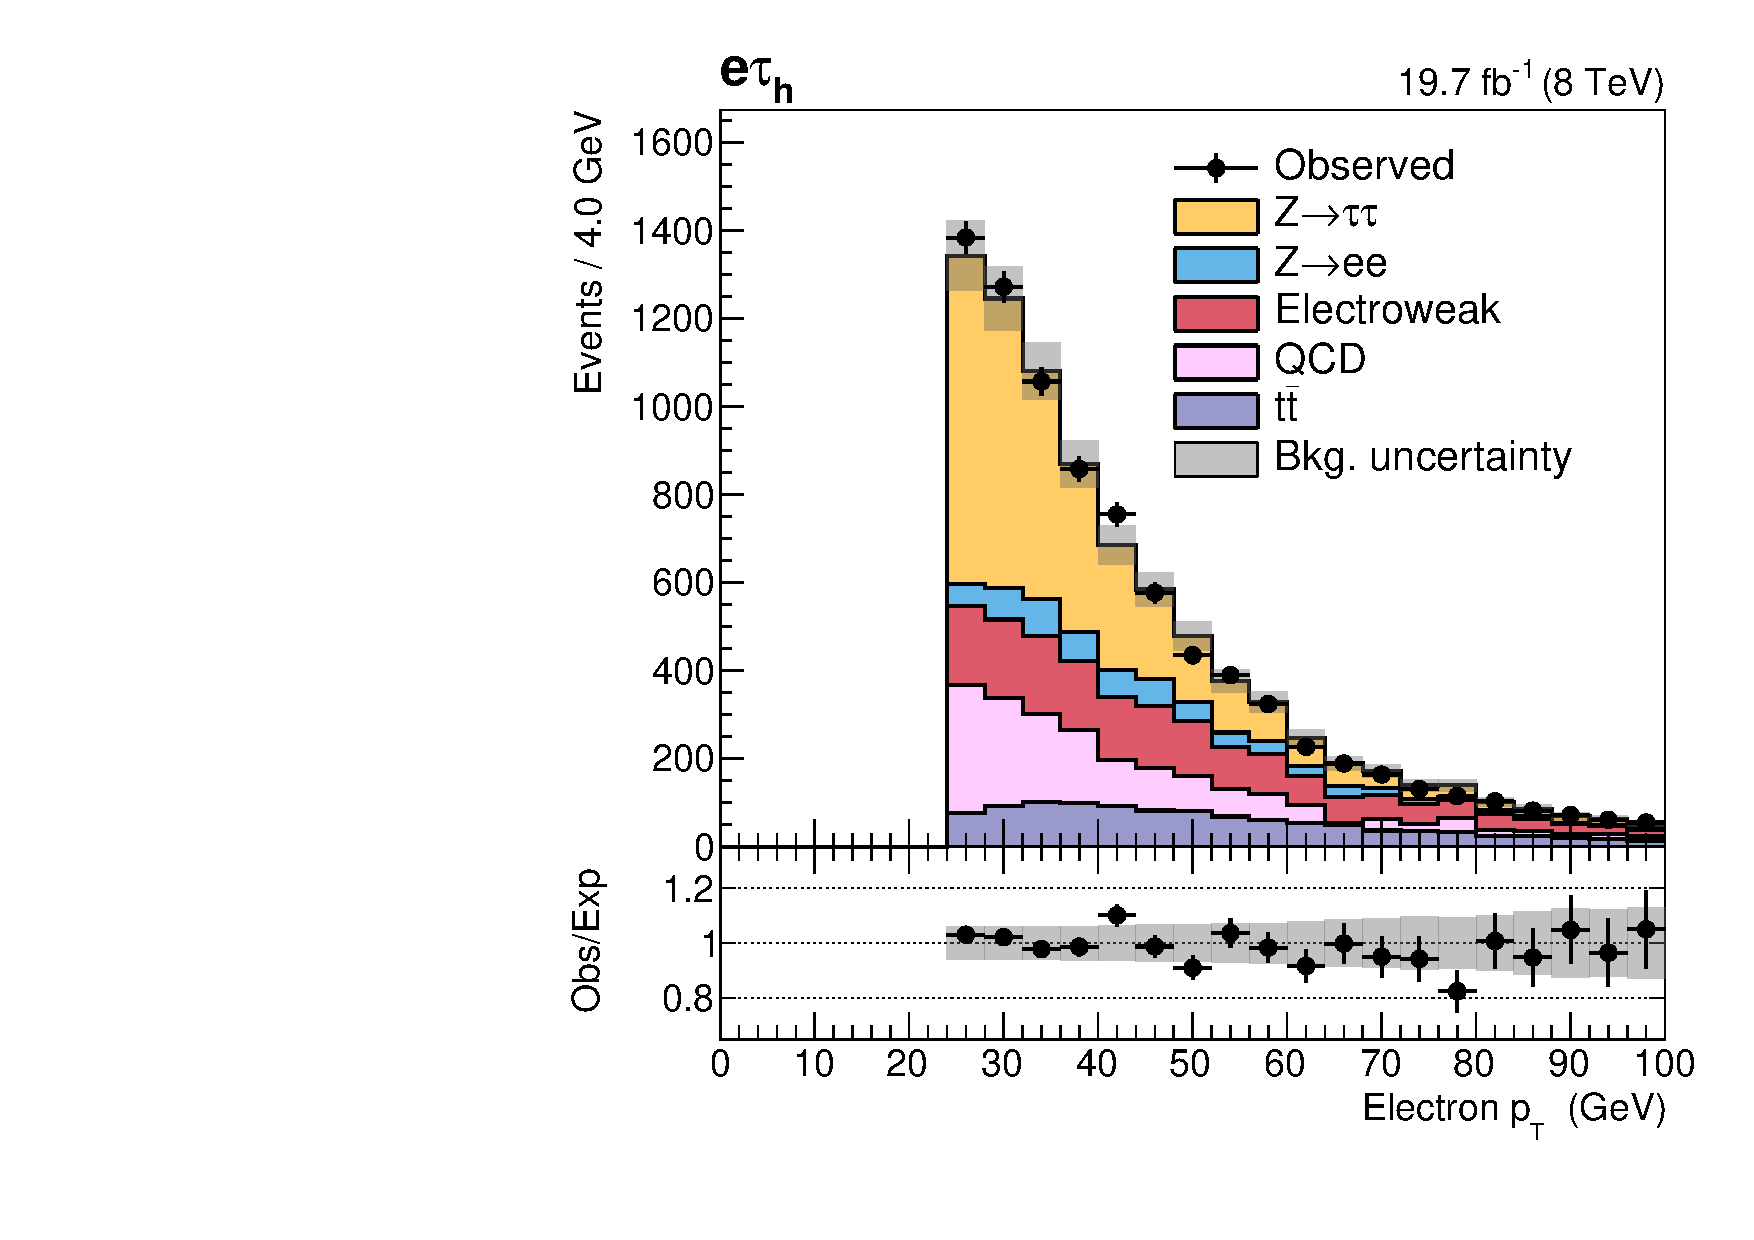
\includegraphics[width=0.5\textwidth]{Hhh/Plots/pt_1_2jetinclusive_et_2012.pdf}}
%  \subfloat[Hadronic \Pgt \pT (\mutau)]{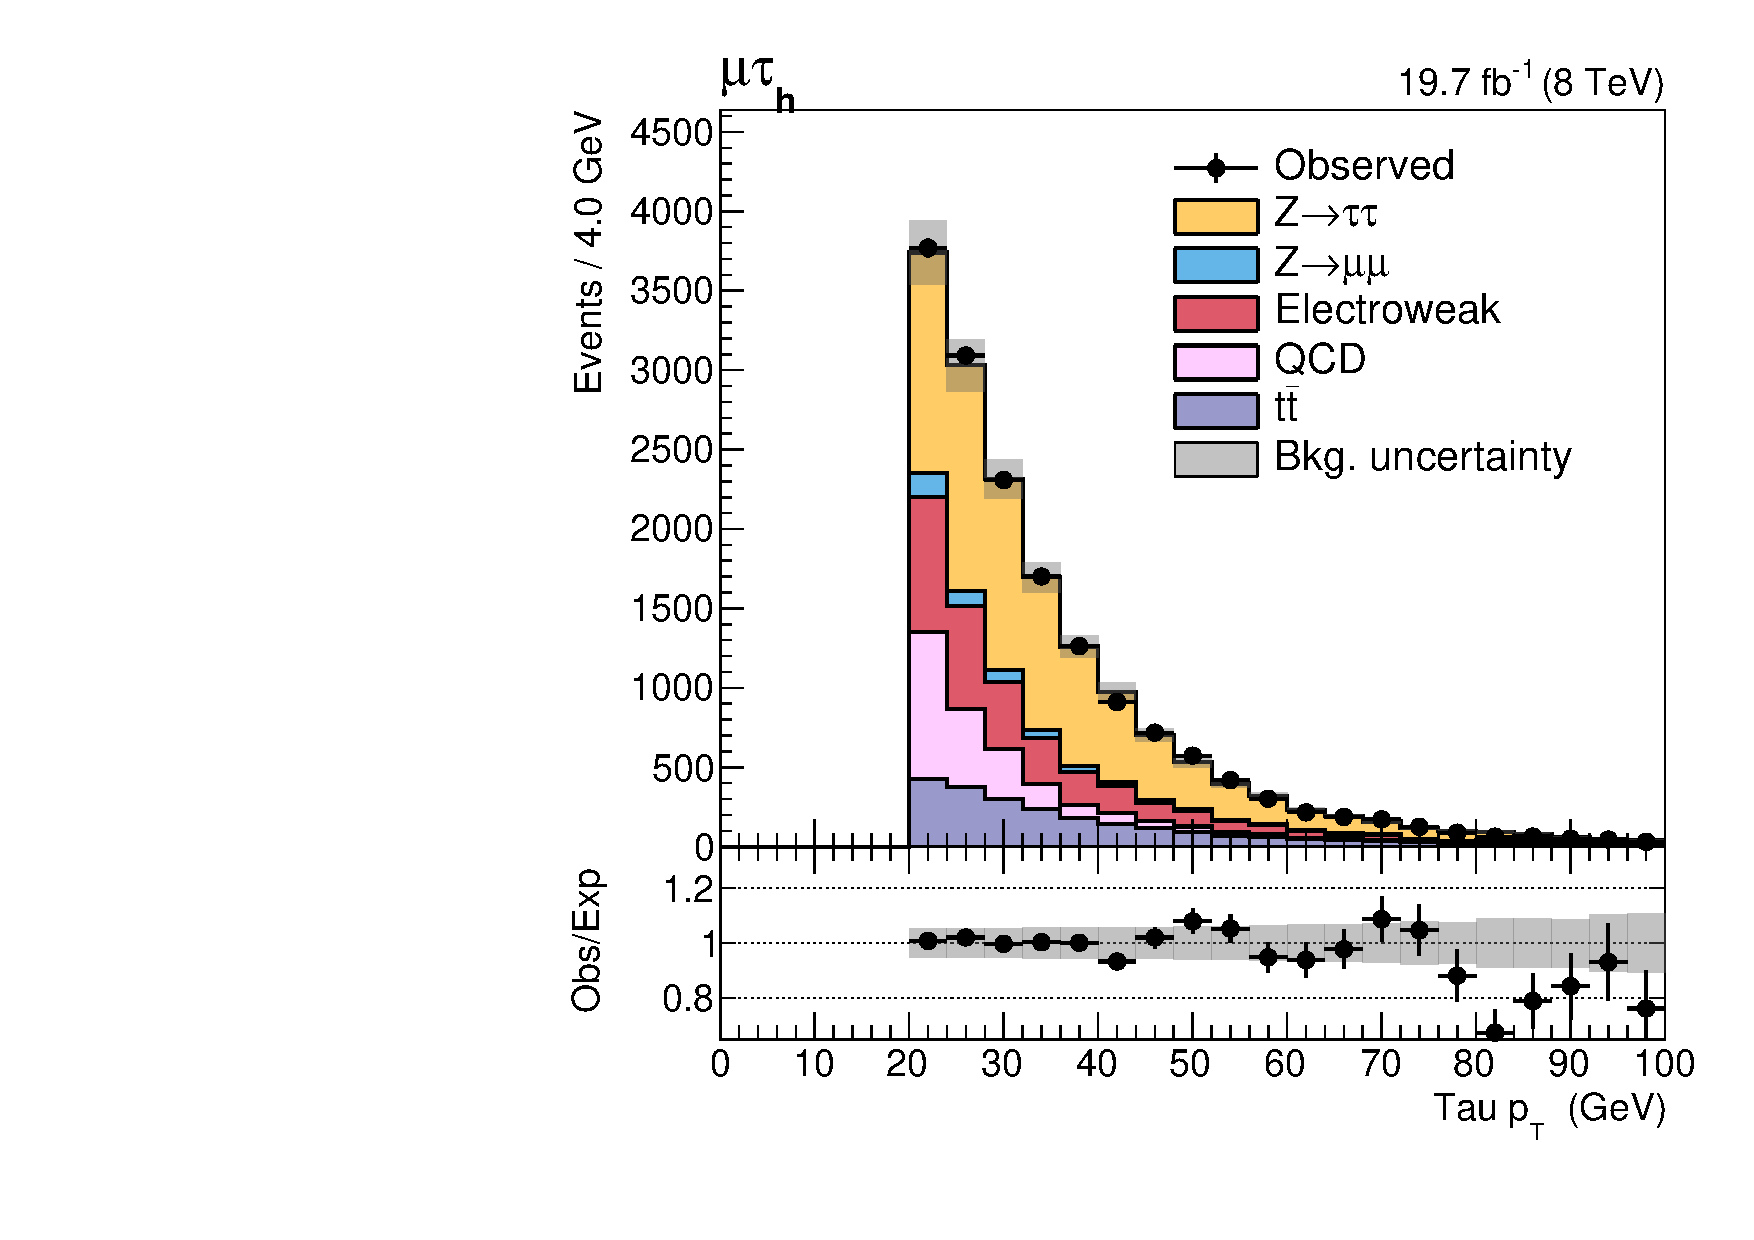
\includegraphics[width=0.5\textwidth]{Hhh/Plots/pt_2_2jetinclusive_mt_2012.pdf}}
%  \subfloat[Electron $\eta$]{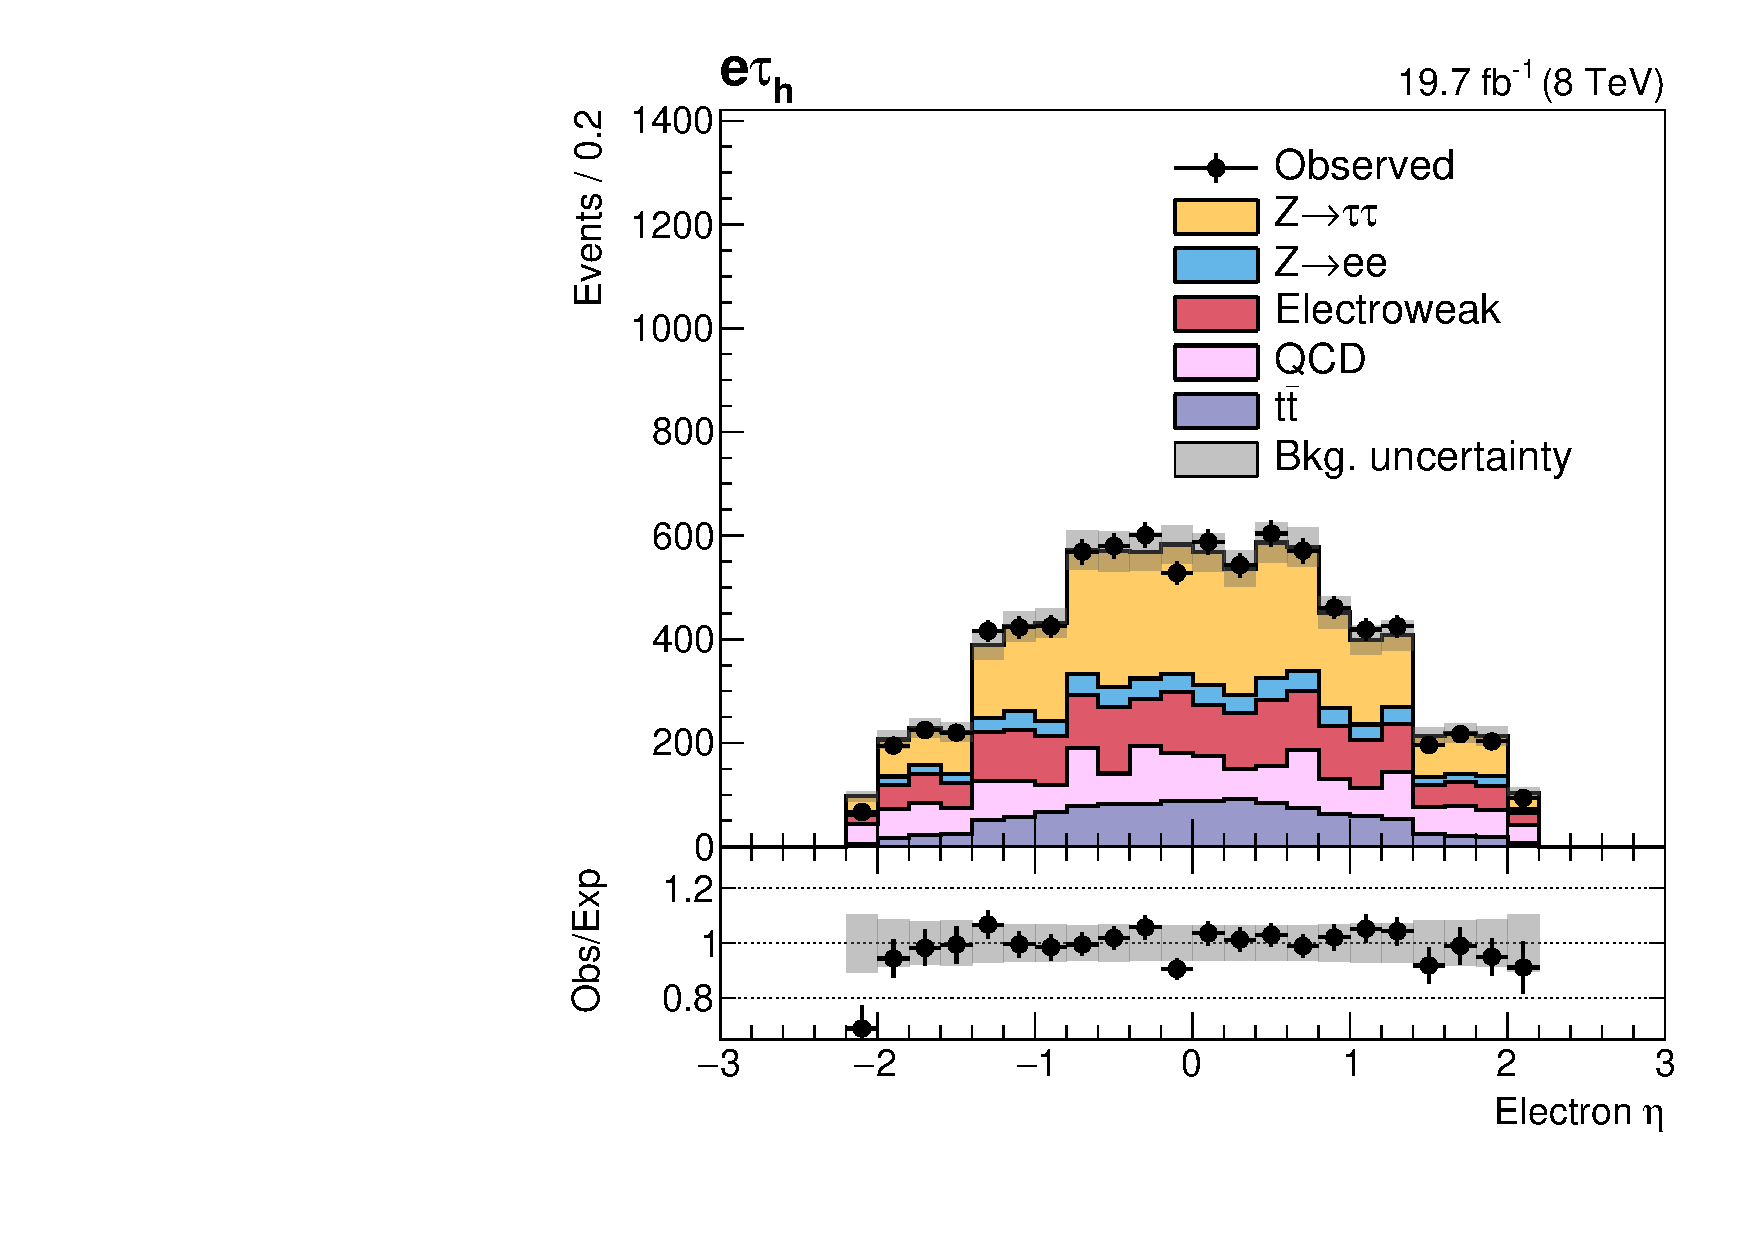
\includegraphics[width=0.5\textwidth]{Hhh/Plots/eta_1_2jetinclusive_et_2012.pdf}}
%  \subfloat[Hadronic \Pgt $\eta$ ]{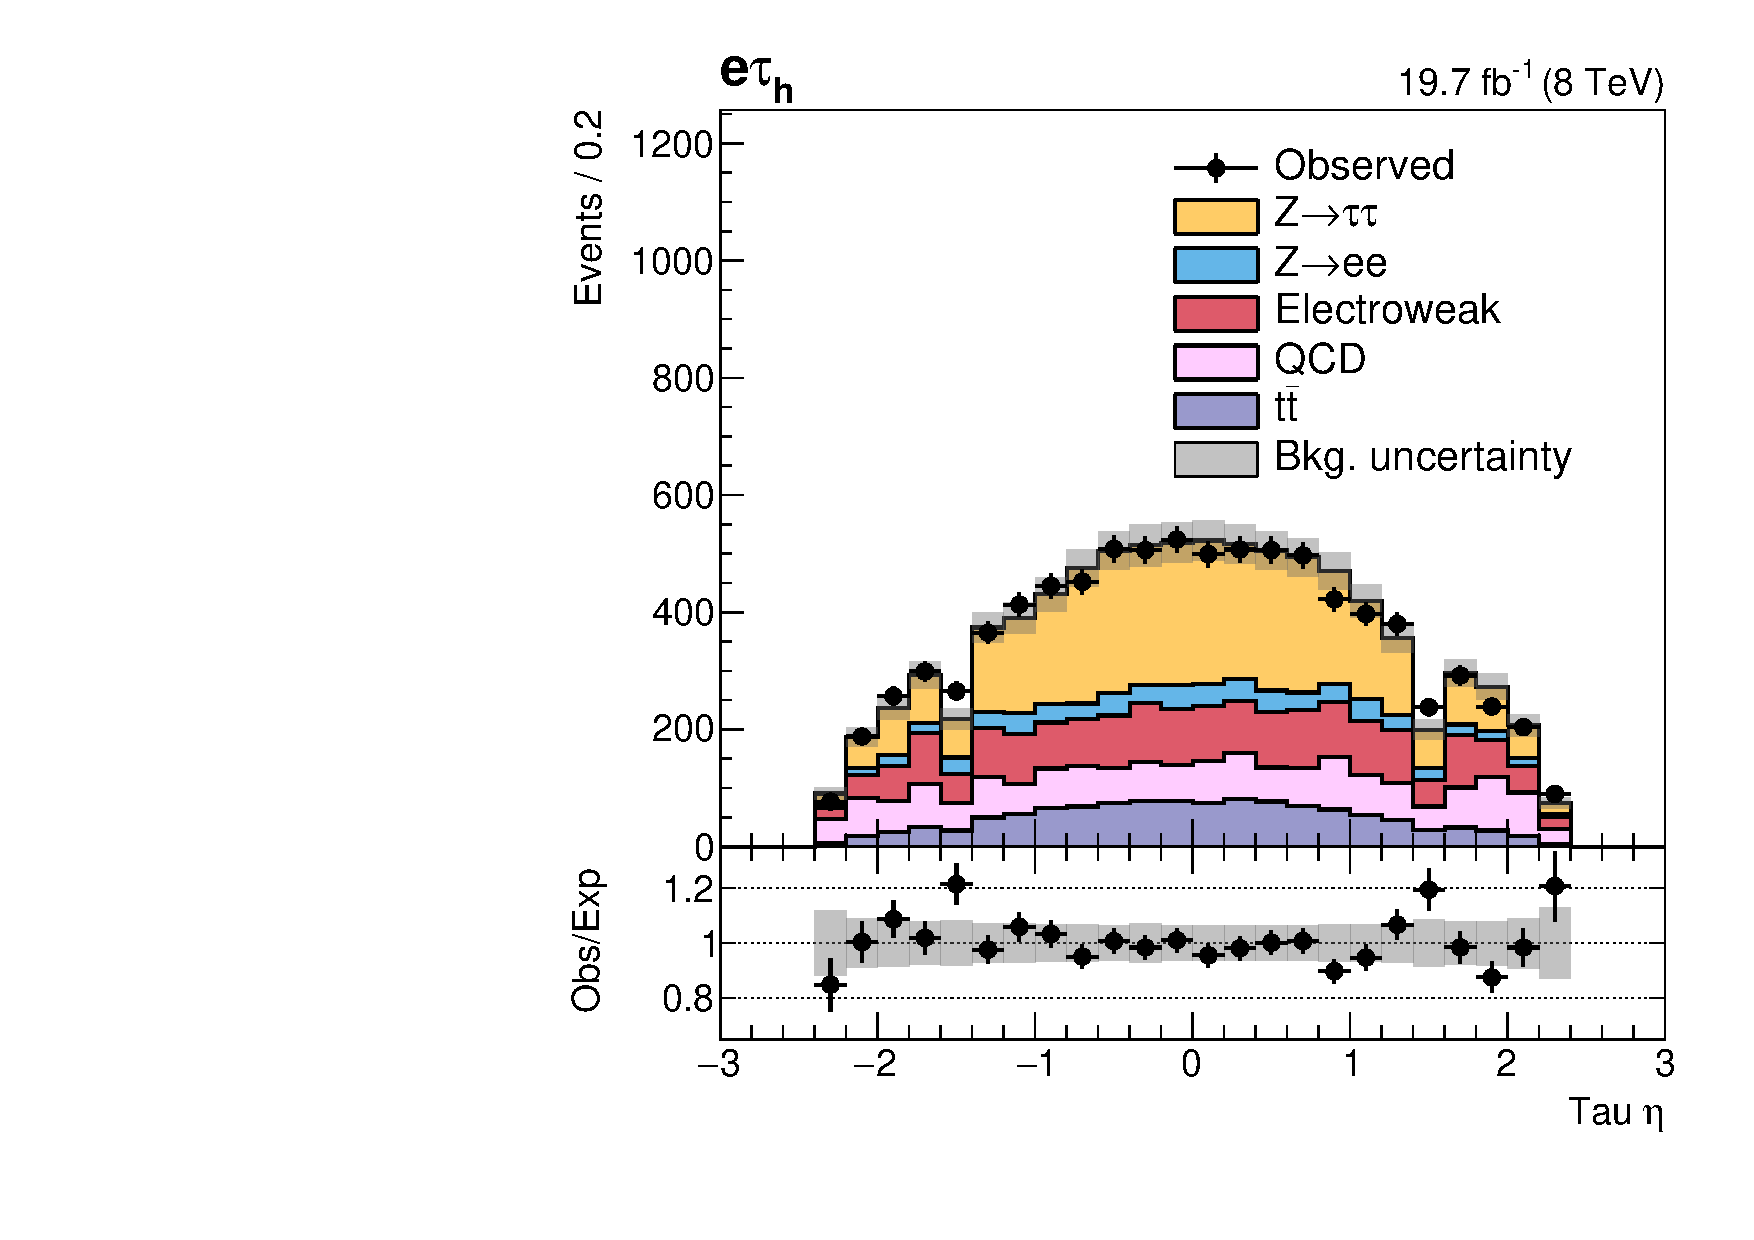
\includegraphics[width=0.5\textwidth]{Hhh/Plots/eta_2_2jetinclusive_et_2012.pdf}}~\\

%\end{center}
%\caption{Plots of electron \pT in the \etau channel and hadronic \Pgt \pT in the \mutau channel.}
%\label{fig:Hhh_selection_kinematics_etmt}
%\end{figure}


\subsection{Categorisation}
\label{sec:hhh_selection_categories}
In both channels a selection on the transverse mass \mT~between the electron/muon
and missing transverse energy, defined as in equation \ref{eqn:hhh_selection_mt}, is applied.
\begin{equation}\label{eqn:hhh_selection_mt}
m_{\text{T}} = \sqrt{2p_{\text{T}}E_{\text{T}}^{\text{miss}}(1-\cos{\Delta\phi})}
\end{equation}
In this eqation \pT~is the transverse momentum of the electron or muon, and $\Delta\phi$ the angle
between the light lepton and the missing transverse energy. The \mT~distributions for the \etau
and \mutau channels, using the selections as
described in sections \ref{sec:hhh_selection_mutau} and \ref{sec:hhh_selection_etau},
are shown in figure \ref{fig:Hhh_selection_mt}.

\begin{figure}[h!]
\begin{center}
\subfloat[\mutau channel]{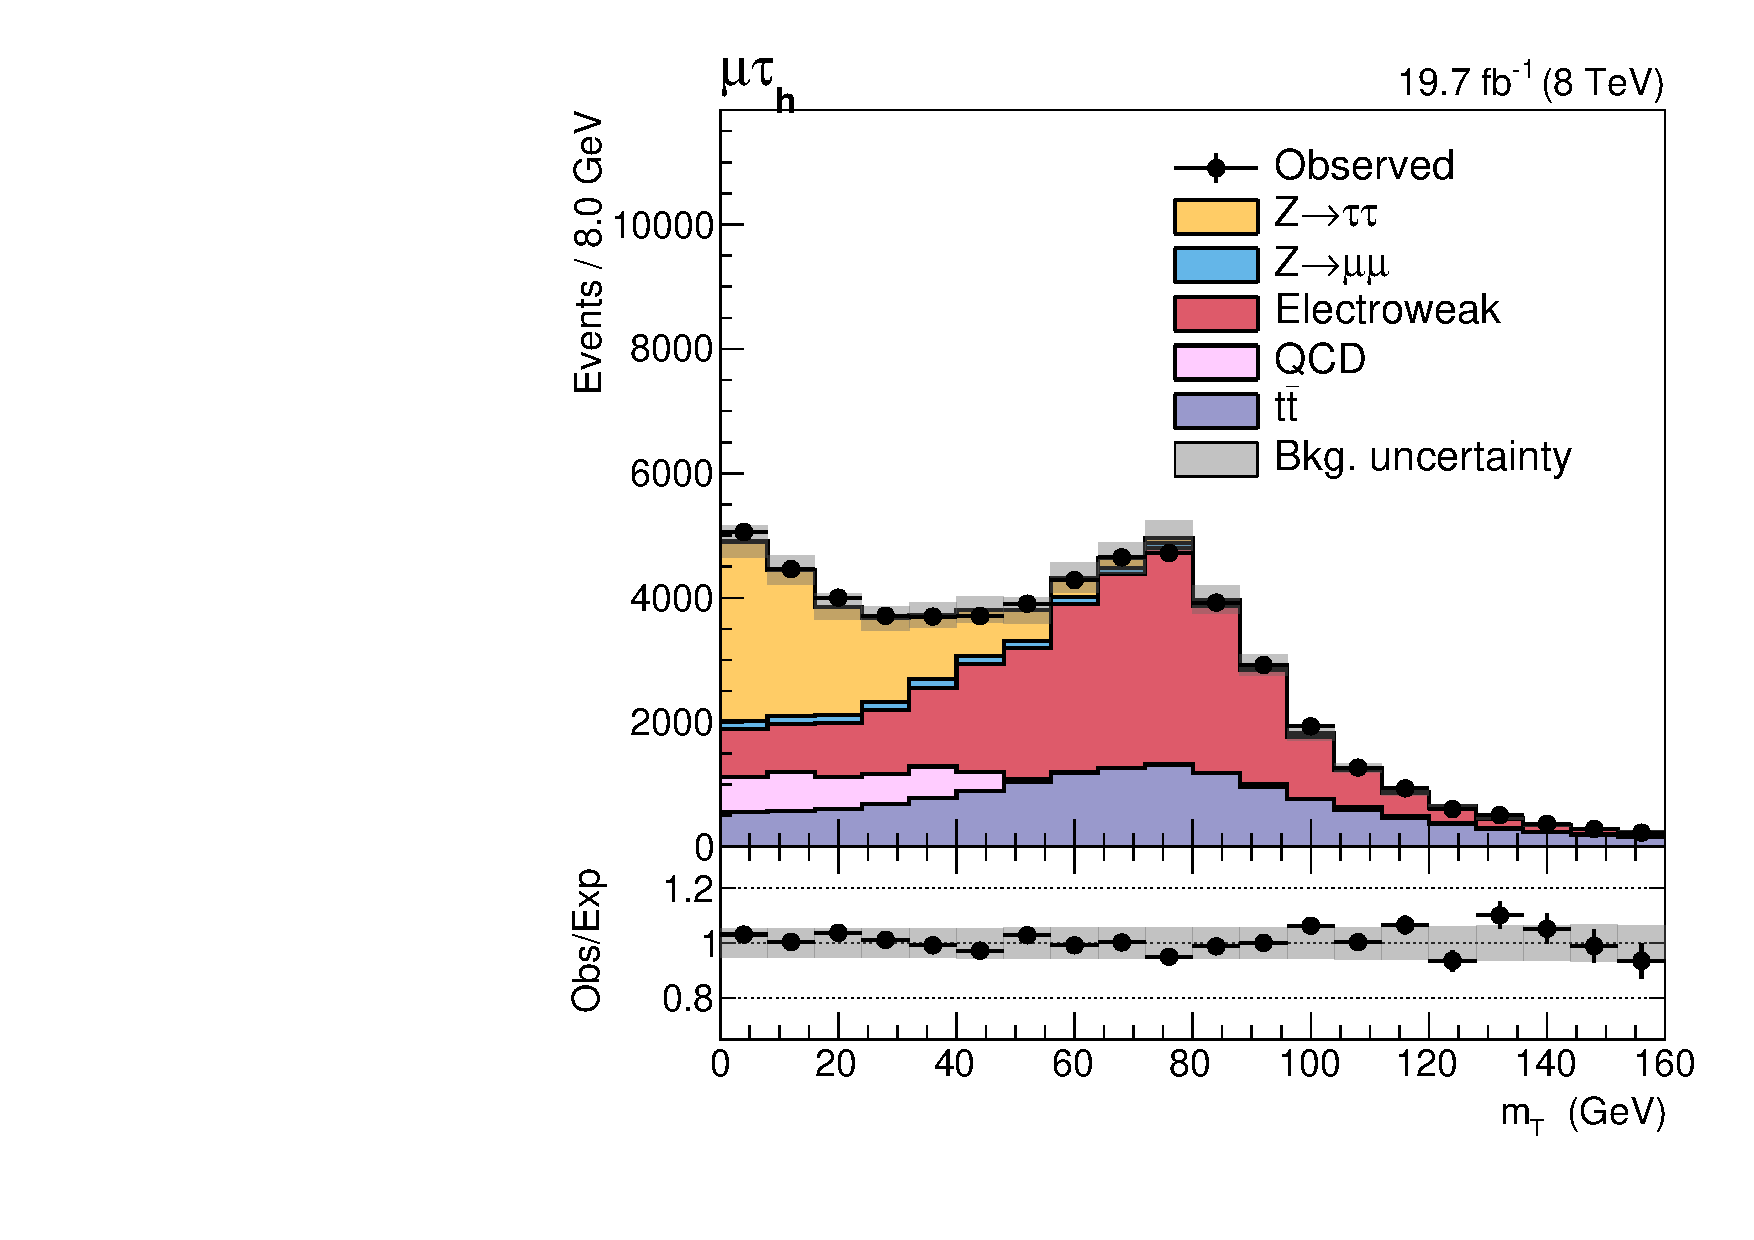
\includegraphics[width=0.5\textwidth]{Hhh/Plots/mt_1_2jetinclusive_mt_2012.pdf}}
\subfloat[\etau channel]{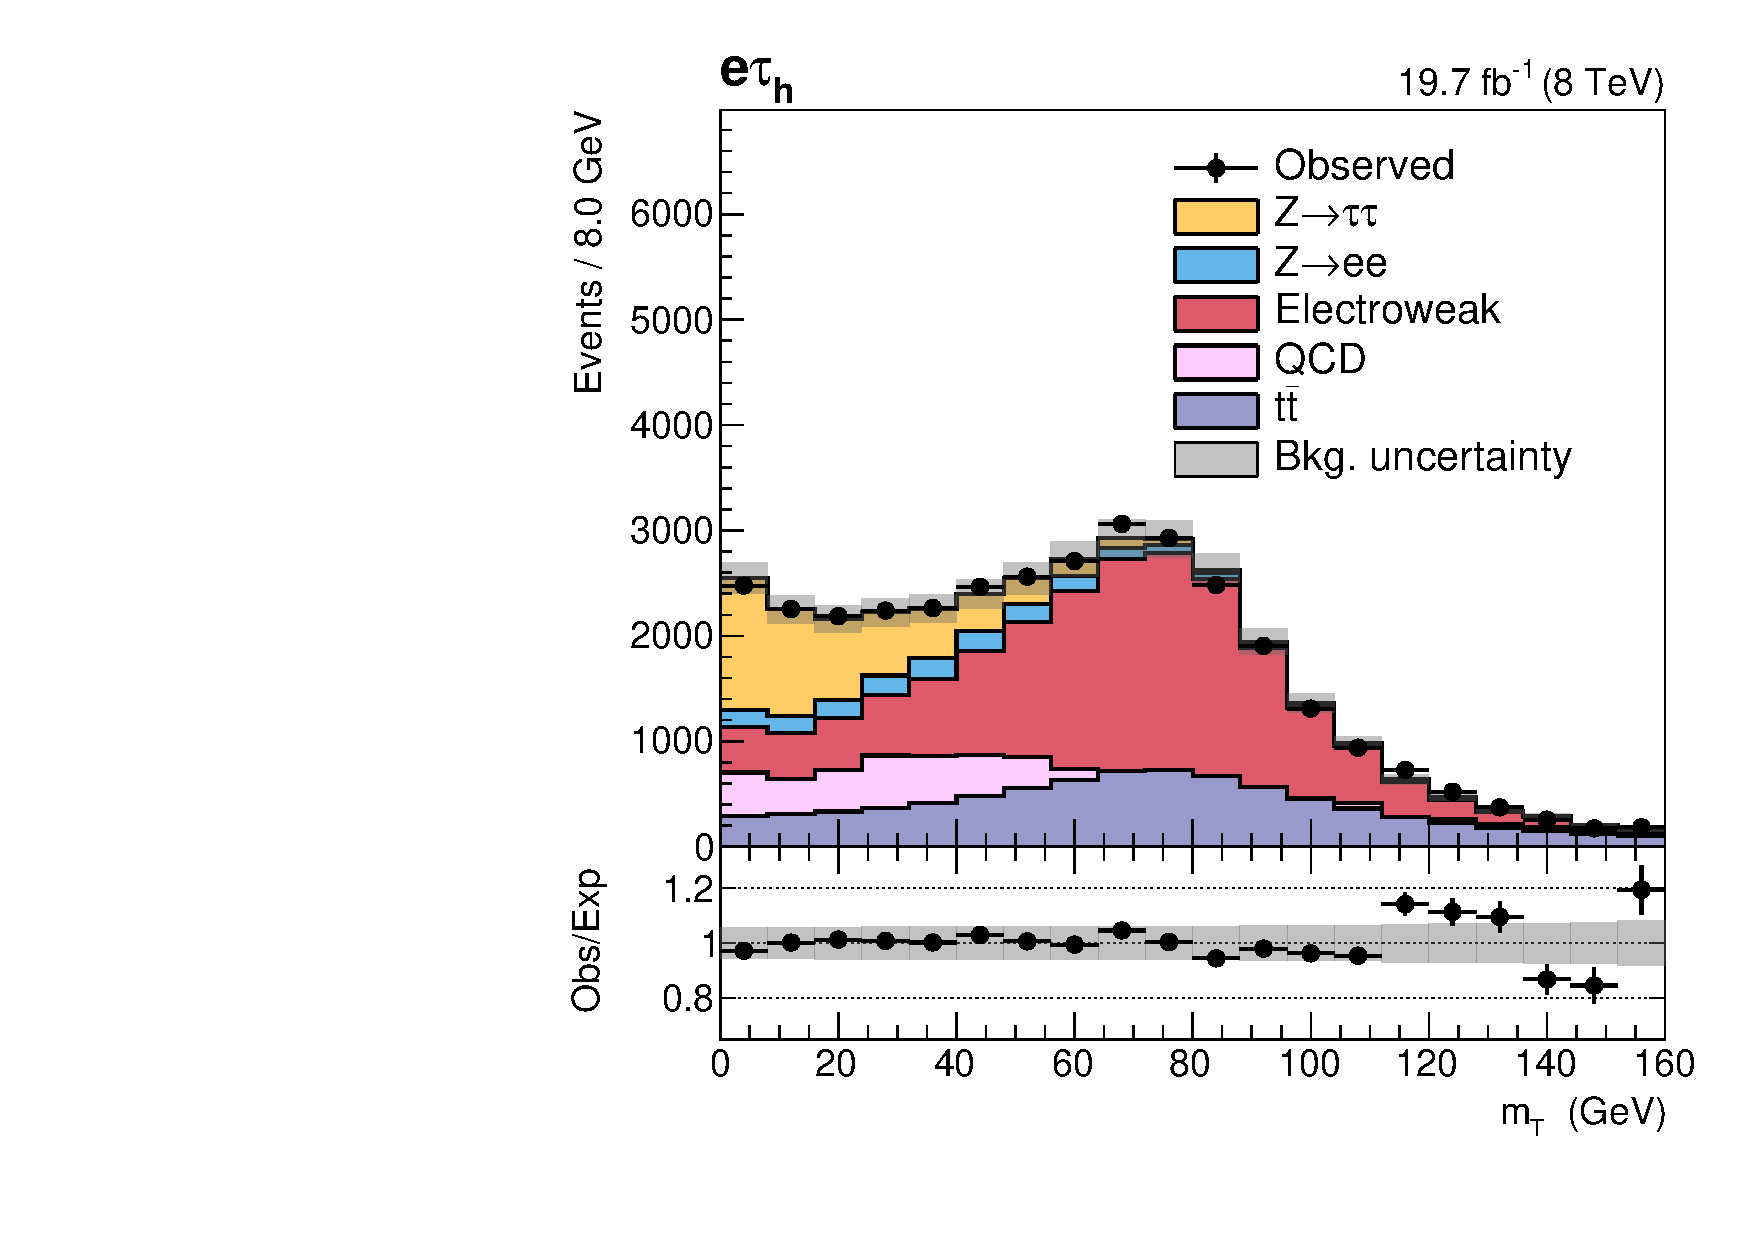
\includegraphics[width=0.5\textwidth]{Hhh/Plots/mt_1_2jetinclusive_et_2012.pdf}}
\end{center}
\caption{\mT~distributions in the \mutau (left) and \etau (right) channels}
\label{fig:Hhh_selection_mt}
\end{figure}

This quantity is required to be smaller than 30 GeV in both channels. In events
where the missing energy and the light lepton are oriented back--to--back, \mT~is
large, whereas it is closer to zero when the two are aligned. In $\PW\rightarrow\ell\nu$
events, as the W is very heavy, the lepton and neutrino are more likely to be emitted back--to--back,
therefore \mT~will be large. For \Ztautau and \htotautau events, in a $\tau\rightarrow\ell\nu\nu$ decay 
the neutrinos are more likely to travel in the same direction as the visible decay products of 
the tau, due to the smaller mass of the \Pgt compared with the \PW. Therefore requiring the
transverse mass to be less than 30 GeV reduces the \Wjets background. This effect
is also visible in figure \ref{fig:Hhh_selection_mt}, where the \Wjets and the much
smaller diboson and single-top backgrounds are combined into the `electroweak' background contribution, drawn in red.
%In this analysis the presence of at least 2 jets increases the relative fraction of \ttbar 
%background events. Because the missing energy can now originate from multiple
%heavy objects (two tops) the missing transverse energy alignment is randomised. In some
%cases the lepton and missing transverse energy can be very much like the W decay
%topology, whereas in other cases \mT will be lower

After applying the \mT~selection, events are divided into three categories to maximise
sensitivity to the signal: 2jet-0tag (at least 2 jets, exactly 0 of which are b-tagged), 2jet-1tag 
(at least 2 jets, exactly 1 of which is b-tagged), 2jet-2tag (at least 2 jets, at least 2 of which are b-tagged).
Jets are considered b-tagged if they pass the medium working point of the b-tagging discriminator described in section OBJECTS.
The 2jet-0tag category does not collect much of the signal and is dominated by 
backgrounds, the 2jet-2tag category is most sensitive to signal. 
Figure \ref{fig:Hhh_selection_bjets}, which shows the number of b-tagged jets in the 2-jet selection of the \mutau and \etau
channels, illustrates this.

\begin{figure}[h!]
\begin{center}
\subfloat[\mutau channel]{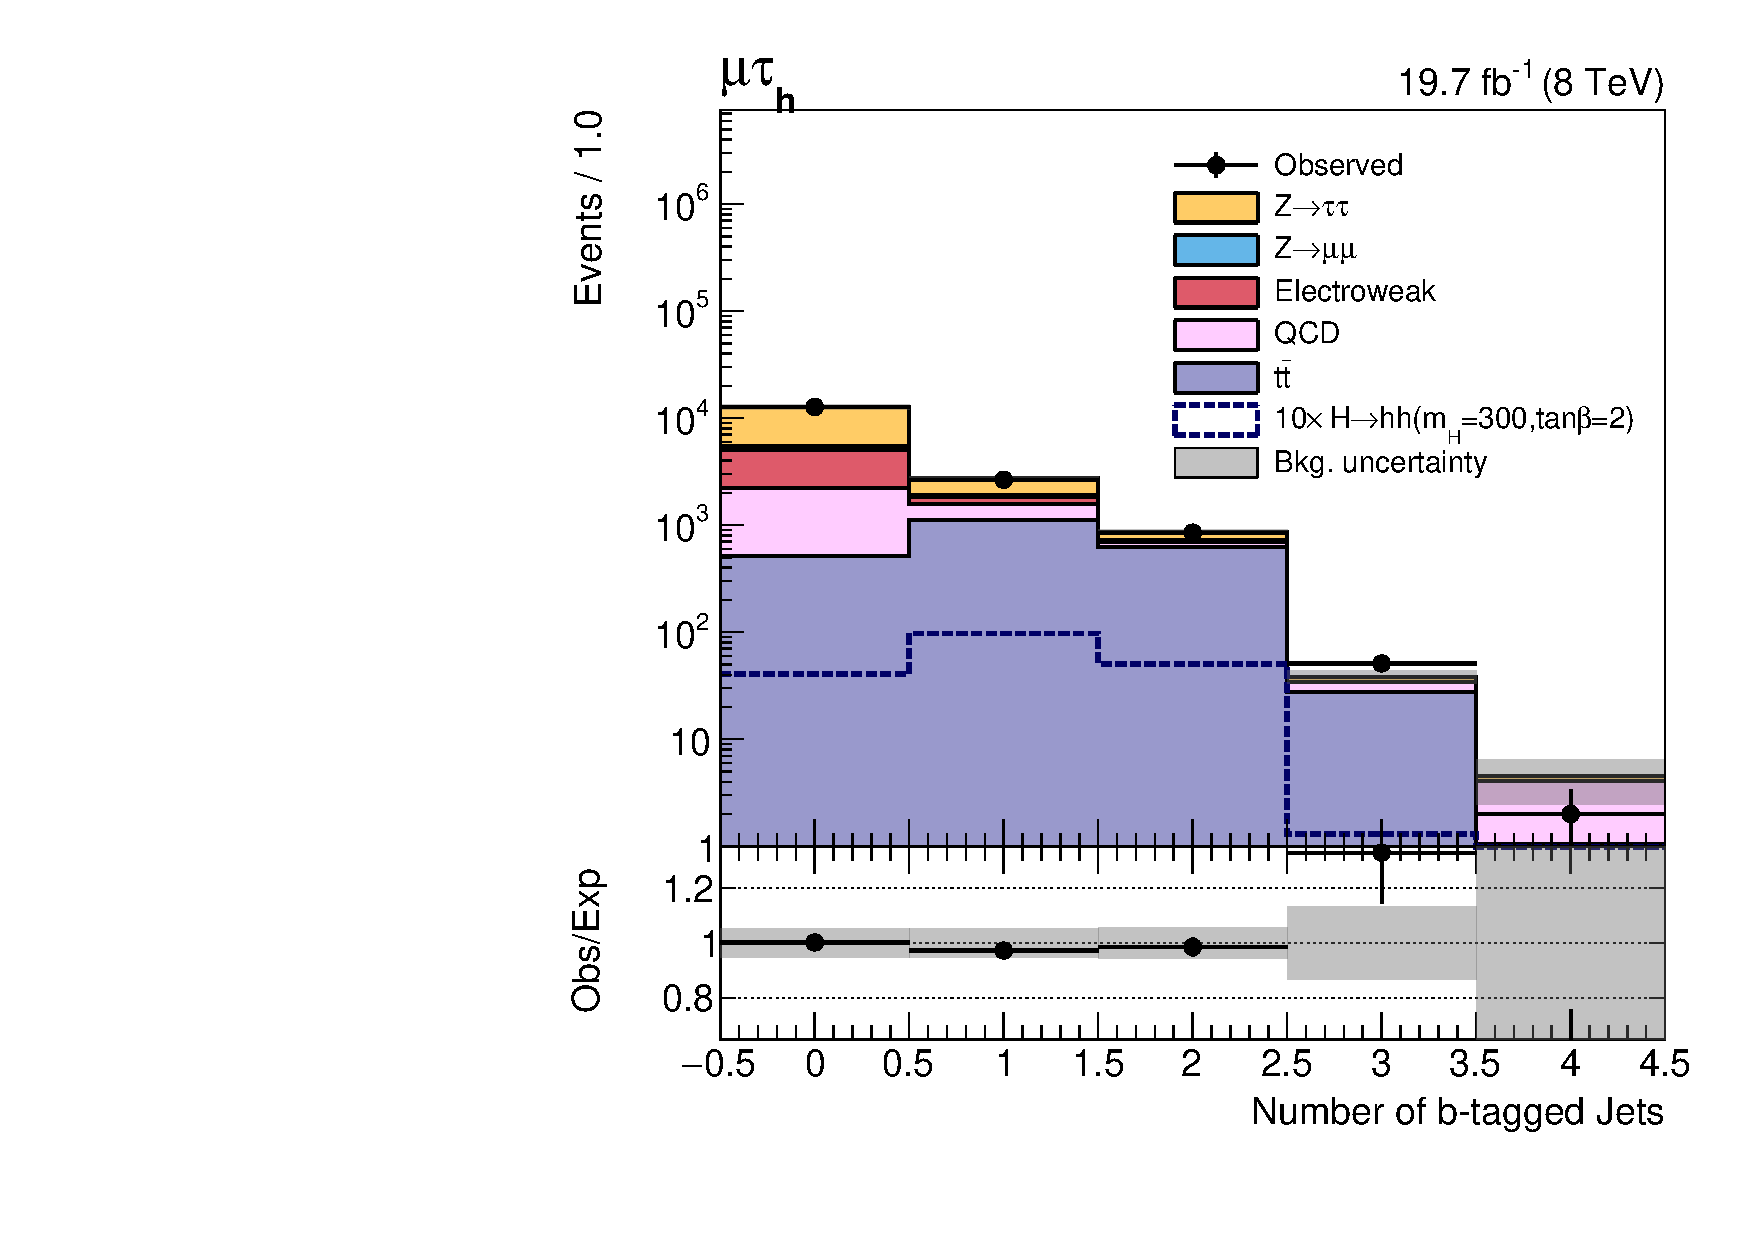
\includegraphics[width=0.5\textwidth]{Hhh/Plots/n_bjets_csv_2jetinclusive_mt_2012_log.pdf}}
\subfloat[\etau channel]{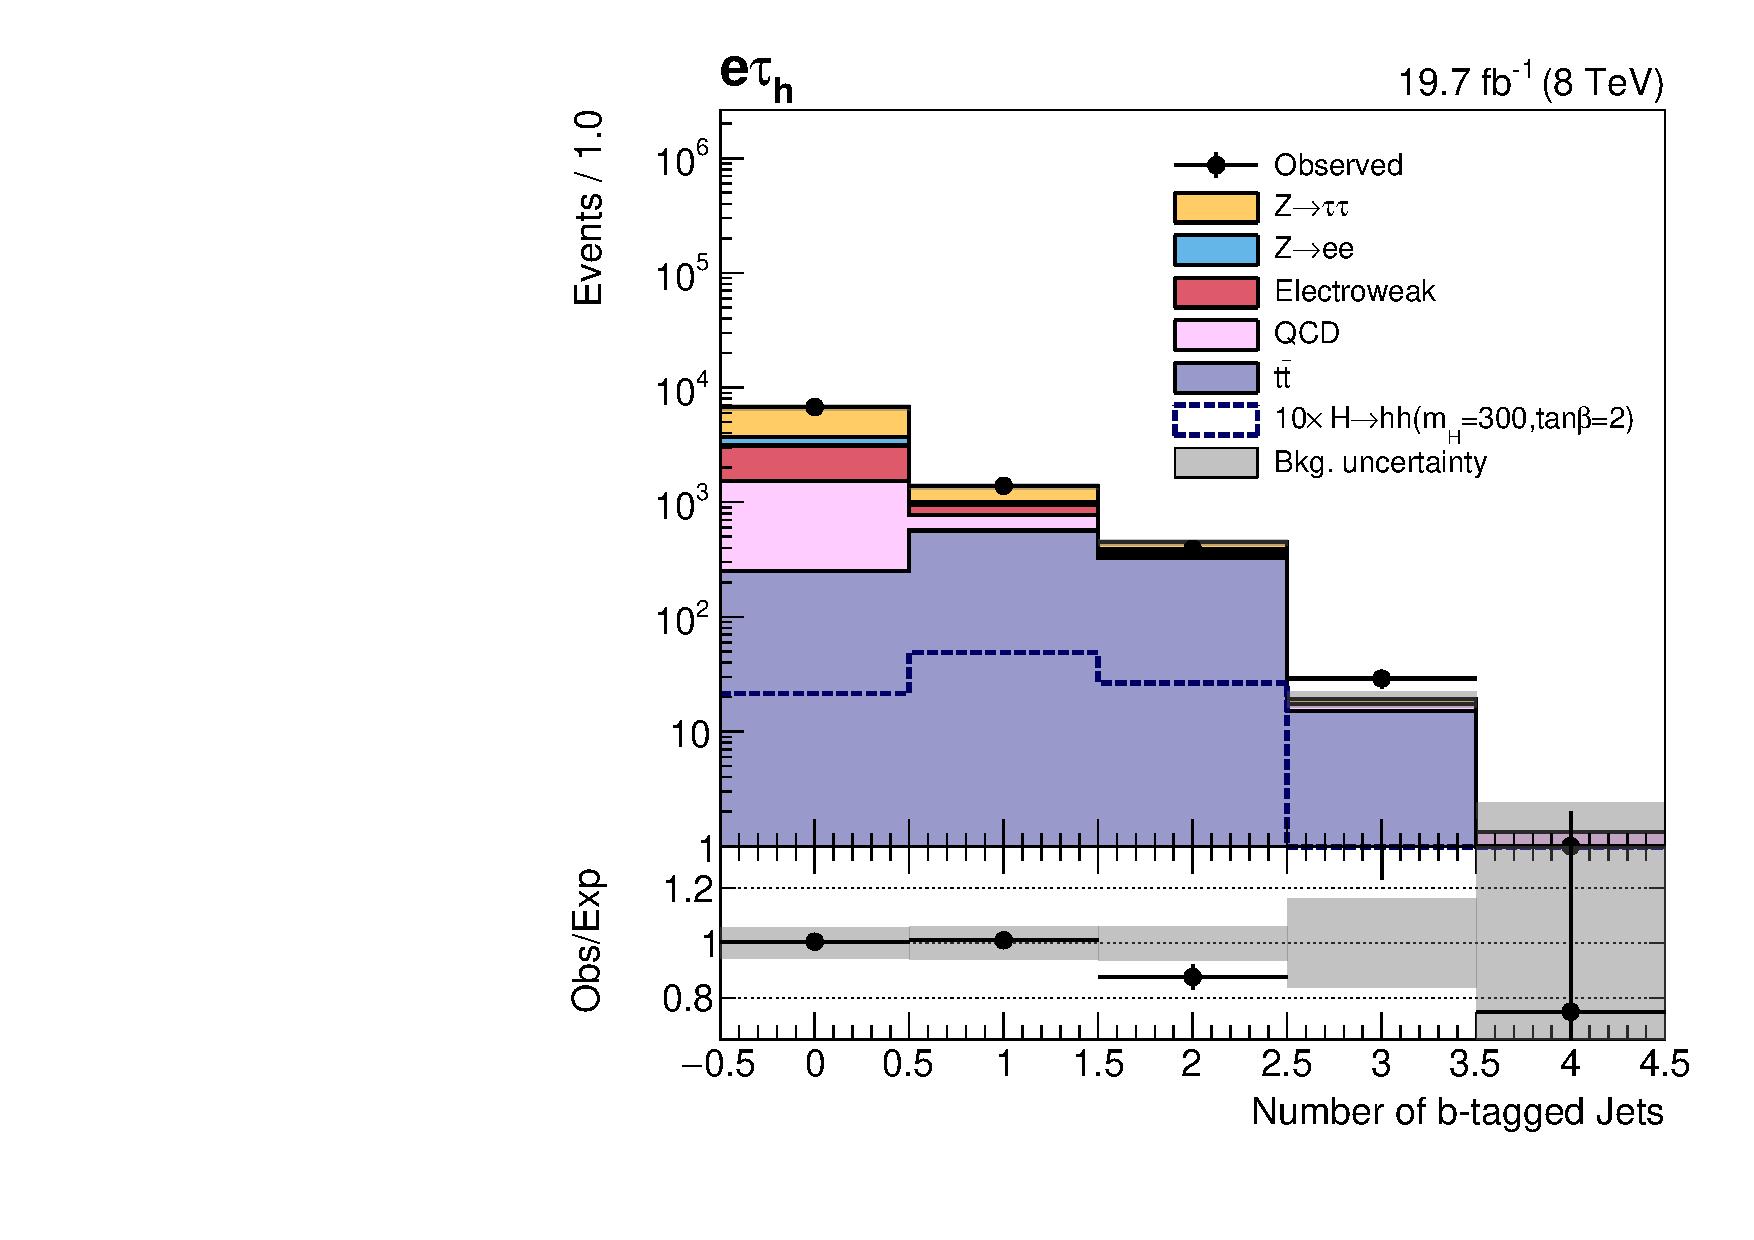
\includegraphics[width=0.5\textwidth]{Hhh/Plots/n_bjets_csv_2jetinclusive_et_2012_log.pdf}}
\end{center}
\caption{Number of b-tagged jets in the 2-jet selection of the \mutau (left) and \etau (right) channels. The signal
at \mH~=$300$~GeV and \tanb~=2, multiplied by a factor of 10, is overlaid on the figures.}
\label{fig:Hhh_selection_bjets}
\end{figure} 

In signal events, the di--tau pair and di--jet pair 
are the decay products of an 125 Gev Higgs boson, therefore their invariant
masses should be close to 125 GeV. To reduce background contributions
from events where the di--tau or di--jet mass is not compatible with
125 GeV, requirements are made on the di--jet invariant mass and the di--tau
invariant mass as reconstructed using the \texttt{SVFit} algorithm \cite{HDiscoveryCMS,SVFit}. This algorithm provides
a likelihood-based estimate of the di-tau mass using the visible decay products
of the taus and the reconstructed \MET. The use of this algorithm greatly
improves the separation between $Z\rightarrow\Pgt\Pgt$ and $H\rightarrow\Pgt\Pgt$ events, 
which is of great importance for the SM $H\rightarrow\Pgt\Pgt$ analysis \cite{HDiscoveryCMS}.
By requiring $70 < m_{jj} < 150 $GeV and $90 < m_{\Pgt\Pgt} < 150$ GeV a 
large number of background events can be rejected, while retaining
most of the signal. This is illustrated in figure \ref{fig:Hhh_selection_masscuts} for 
the 2jet-2tag category.

\begin{figure}[h!]
\begin{center}
\subfloat[$m_{\Pgt\Pgt}$]{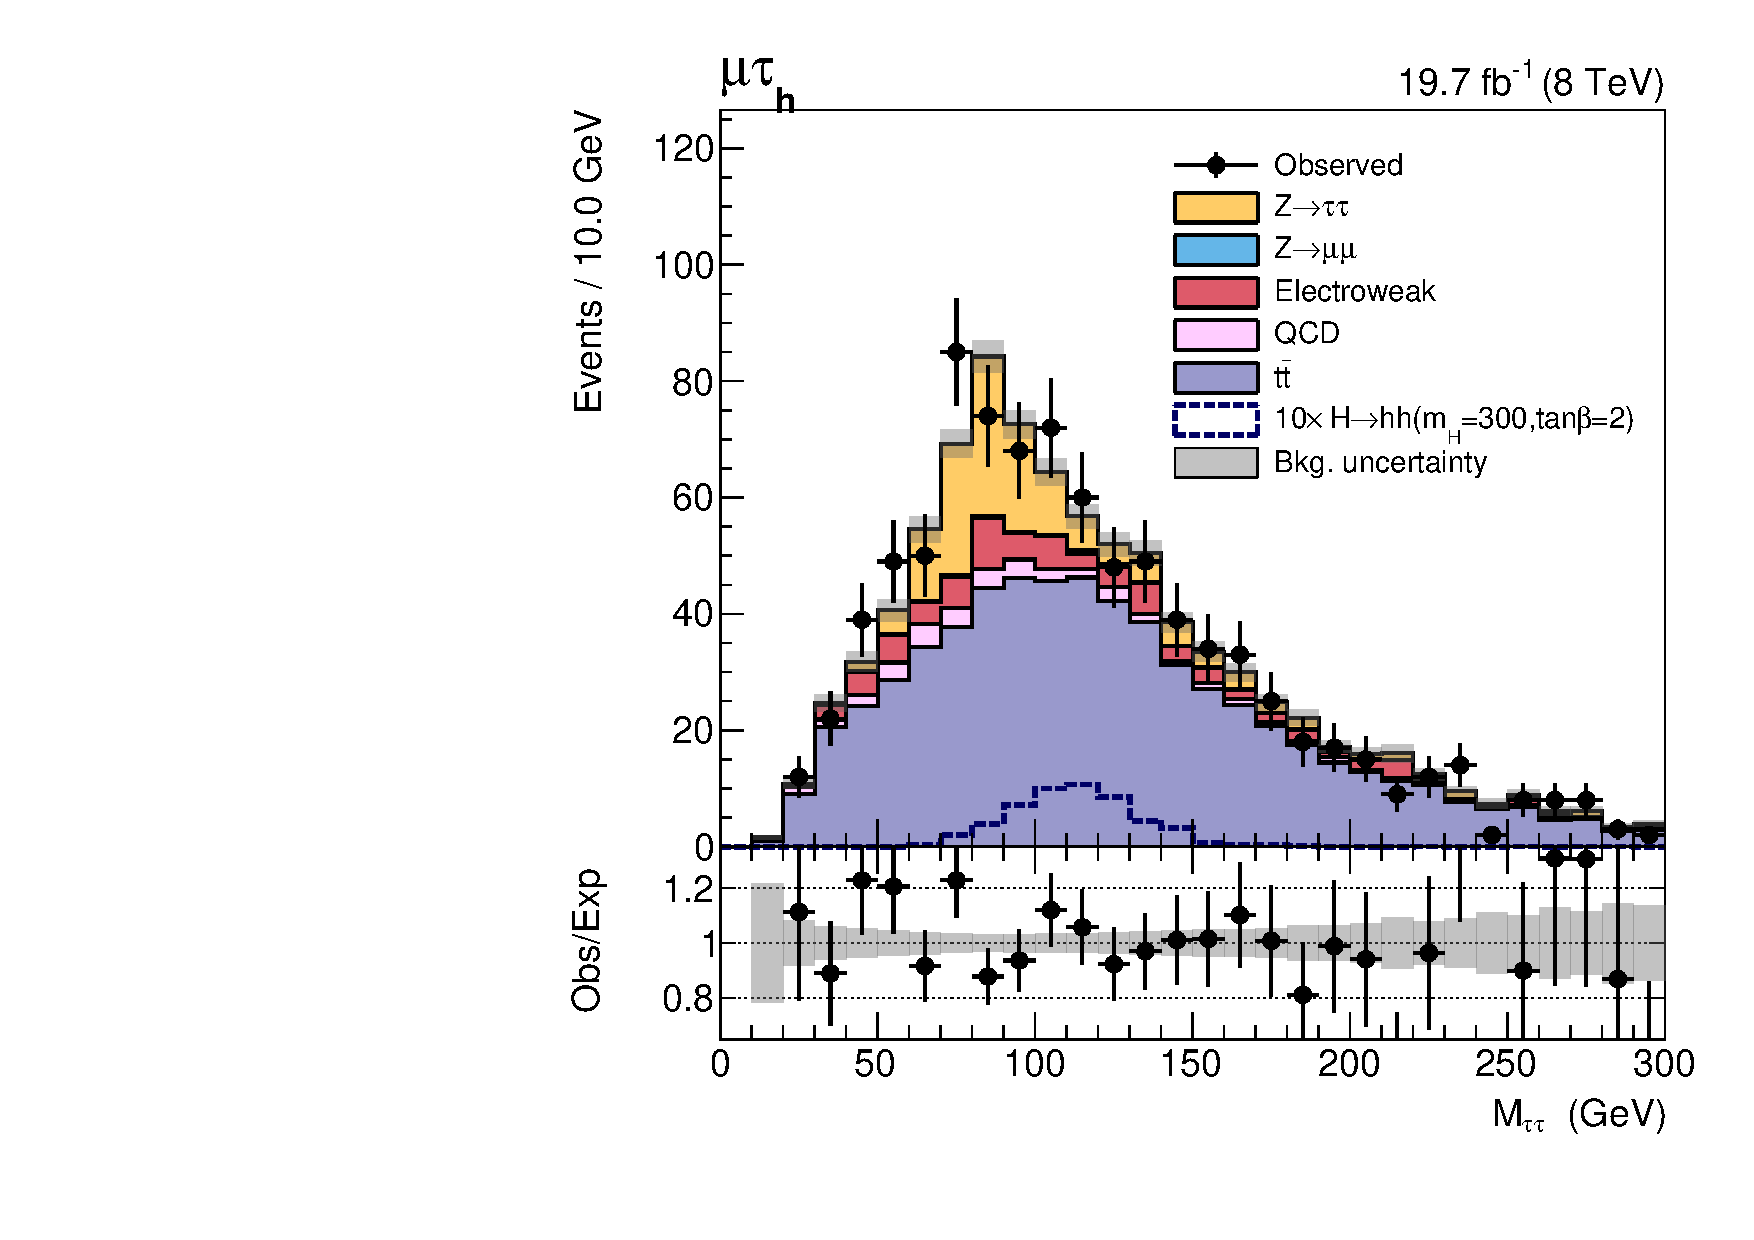
\includegraphics[width=0.5\textwidth]{Hhh/Plots/m_sv_2jet2tag_mt_2012.pdf}}
\subfloat[$m_{jj}$ ]{\includegraphics[width=0.5\textwidth]{Hhh/Plots/mjj_2jet2tag_mt_2012.pdf}}
\end{center}
\caption{Reconstructed di-\Pgt invariant mass (left) and di-jet invariant mass (right) in the 2jet-2tag category of the \mutau
channel. The signal for a heavy Higgs boson H with mass \mH = 300 GeV at \tanb=2 in the low \tanb~ MSSM scenario, enlarged by a factor 10, is overlaid on the figures.
In both variables the signal peaks at around 125 GeV.}
\label{fig:Hhh_selection_masscuts}
\end{figure}

\section{\acl{MC} to data correction factors}
\label{sec:hhh_datamc}
\ac{MC} samples are used for the estimation of some of the backgrounds and the signal, 
and it is therefore important to correct for any mismodelling. The \ac{MC} to data 
correction factors used for this are estimated in dedicated control regions.

A reweighting is applied to make the pile--up distribution in \ac{MC}
match the distribution observed in data, as described in chapter OBJECTS.

Data and \ac{MC} identification, isolation, and trigger efficiencies
are measured for electrons, muons and hadronic taus. The difference between
the efficiencies in data and \ac{MC} are applied to \ac{MC} events as a
scale factor $SF = \frac{\epsilon_{\text{Data}}}{\epsilon_{\text{MC}}}$.

For electrons and muons, these efficiencies are measured using a 
tag--and--probe method using \Zeenog and \Zmmnog events, respectively.
The hadronic tau identification, isolation and trigger efficiencies
are measured via a similar method that makes use of
$Z\rightarrow\Pgt\Pgt\rightarrow\Pgm\Pgt_{h}$ events.

The energy scale for hadronic taus is determined by fitting the mass of the 
hadronic tau candidate in $Z\rightarrow\Pgt\Pgt\rightarrow\Pgm\Pgt_{h}$ events.
This fit is performed separately for each hadronic tau decay mode to obtain
an energy scaling that is applied to reconstructed hadronic taus matched
to generator-level hadronic tau decays in MC events.

In the \etau channel a \ac{MC} to data scale factor is applied
to the \Zee background, to correct for differences in the $e\rightarrow\Pgt_{h}$
fake rate between data and \ac{MC}. This scale factor is derived separately
for the 1-prong + 0$\pi^0$ hadronic tau decay mode, and 1-prong + at least one
$\pi^0$ decay modes by fitting the visible mass of the \Pe+$\Pgt_{h}$ pair
in events passing the selection of the \etau channel as described in section
\ref{sec:hhh_selection_etau}, with the 2-jet requirement lifted.

Differences in \MET resolution and response between data and \ac{MC} are accounted for by
applying Z--recoil corrections to DY, \Wjets and signal \ac{MC} events. Chapter OBJECTS
gives more details on how these corrections are derived.

To correct for the difference in b--tagging efficiency and light jet mis--tagging
rates between data and \ac{MC} \pT~and $\eta$~dependent scale factors are 
derived using the method described in \cite{BTV8TeV}. There are separate scale factors for 
b-/c- jets and light jets. Multiple possible ways to apply these scale factors
exist, for this analysis this is done through a promote/demote method.

In this method a demotion or promotion probability is assigned to every
jet as in equation \ref{eqn:promotedemote}.
\begin{align}\label{eqn:promotedemote}
&P(\text{demote}) = 1 - SF \text{  for SF < 1 }  \notag \\
&P(\text{promote}) = \frac{(SF - 1)(\epsilon_{\text{MC}}-1)}{SF} \text{    for SF > 1}
\end{align}
In this equation $SF$ is the scale factor mentioned above, and $\epsilon_{\text{MC}}$ is
the b--tagging efficiency in \ac{MC} events for the type of jet (light, b- or c-)
in consideration.

\section{Discriminating variable}
\label{sec:hhh_discr}
The variable of interest in this analysis is the mass of the heavy Higgs boson H. This can be
reconstructed as the 4--body mass of the two jets and the two taus, however
a more accurate result can be obtained by using a kinematic fitting 
procedure that makes use of the 125 GeV mass constraint on the di--tau and
di--jet candidates. 

In a kinematic fit constraints are made on the event kinematics, in the
case of this analysis these constraints are
$m(\Pgt_{1},\Pgt_{2}) = m_{h} = 125 $~GeV and
$m(b_{1},b_{2}) = m_{h} = 125 $ GeV.
The kinematic observables related to the hadronic taus and jets
are varied within their uncertainties to fulfill these 
constraints. A $\chi^2$ cost term is introduced for each
observable that is varied with respect to the measurement,
the aim of the fit is to minimise the sum of these $\chi^2$ terms.

For b-jets, the reconstructed direction in $\eta$ and $\phi$ is 
assumed to be measured accurately in comparison with their energy.
Therefore only their energy is varied in the fit. In addition, we assume
that uncertainties in the energy measurement directly translate to
uncertainties in the momentum measurement, therefore $\vec{\beta} = \vec{p}/E$ is
also kept constant. 

Before the fit, from the mass constraint we have (equation \ref{eqn:kinfit_prefit})
~\vspace{-0.5\baselineskip}
\begin{align}\label{eqn:kinfit_prefit}
m_{h}^2 &= E_{h}^2 - \vec{p_{h}}^2 = (E_{b1}+E_{b2})^2 - (\vec{p_{b1}} + \vec{p_{b2}})^2 \notag\\
& = 2E_{b1}E_{b2} + m_{b1}^2 +m_{b2}^2 - 2\vec{p_{b1}}\vec{p_{b2}} \notag\\
& = m_{b1}^2 +m_{b2}^2 - 2E_{b1}E_{b2}(1-\vec{\beta_{b1}}\vec{\beta_{b2}})\notag\\
&\Rightarrow (1-\vec{\beta_{b1}}\vec{\beta_{b2}}) = \frac{m_h^2 - m_{b1}^2 - m_{b2}^2}{2E_{b1}E_{b2}}
\end{align}
When varying the energy of the first jet in the fit, equation \ref{eqn:kinfit_prefit} can be 
rewritten to derive an expression for the updated energy of the second jet. Using $\mathcal{A} = (1-\vec{\beta_{b1}}\vec{\beta_{b2}})$ 
and equation \ref{eqn:gamma_def}:
~\vspace{-0.5\baselineskip}
\begin{equation}\label{eqn:gamma_def}
\gamma = \frac{1}{1-\beta^2} \Rightarrow \gamma^2 = \frac{1}{1-\beta^2} = \frac{1}{1-p^2/E^2} = \frac{E^2}{m^2}
\end{equation}
We get:
~\vspace{-0.5\baselineskip}
\begin{align}\label{eqn:kinfit_variation}
m_h^2 &= m_{b1}^2 + m_{b2}^2 - 2E_{b1}E_{b2}(1-\vec{\beta_{b1}}\vec{\beta{b2}})\notag\\
&= m_{b1}^2 +\frac{E_{b2,fit}^2}{\gamma_{b2}^2} +2\mathcal{A}E_{b1}E_{b2,fit}\notag\\
\Rightarrow E_{b2}^{fit}& = \frac{(-2E_{b1}\mathcal{A} + \sqrt{4E_{b1}^2\mathcal{A} - 4(m_{b1}^2-m_{h}^2)\gamma_{b2}^{-2}})\gamma_{b2}^2}{2}\notag\\
&= - E_{b1}\mathcal{A}\gamma_{b2}^2+\sqrt{E_{b1}^2\mathcal{A}\gamma_{b2}^4 - (m_{b1}^2 - m_{h}^2)\gamma_{b2}^2}\notag\\
&\Rightarrow E_{b2}^{fit} = E_{b1}\mathcal{A}\gamma_{b2}^2(-1 + \sqrt{1+\frac{m_{h}^2 - m_{b1}^2}{E_{b1}^2\mathcal{A}\gamma_{b2}^2}})
\end{align}

The fitting procedure additionally modifies the masses of the b-jets as (equation \ref{eqn:kinfit_bjetmass})
~\vspace{-0.5\baselineskip}
\begin{equation}\label{eqn:kinfit_bjetmass}
m_{b_{1,2}}^{fit} = m_{b_{1,2}}\frac{E_{b_{1,2}}^{fit}}{E_{b_{1,2}}}
\end{equation}
The $\chi^2$ term for each b-jet is calculated as $\chi_{b1,2}^2 = \frac{E_{b1,2}^{fit}-E_{b1,2}^{meas}}{\sigma_{b1,2}}$.

For taus only the visible decay products are measured. Assuming the visible decay products of the \Pgt point in 
the same direction as the original \Pgt, a similar procedure as for the b-jets can be employed to constrain the mass of the second tau
when varying the mass of the first tau in the fit. The masses of the taus are kept fixed at $m_{\Pgt}$ throughout the procedure.

Due to the missing energy associated with the \Pgt decays, additional constraints
on the fit have to be used to reconstruct the correct tau energies. This is done by 
enforcing that the heavy Higgs boson recoil from the fit is close to the reconstructed recoil.

The measured recoil is (equation \ref{eqn:kinfit_recoilmeas})
~\vspace{-0.5\baselineskip}
\begin{equation}\label{eqn:kinfit_recoilmeas}
\vec{p_{\text{T,recoil}}}^{\text{meas}} = -\vec{p_{\text{T,H}}}^{\text{meas}} = -\vec{p_{\text{T,miss}}}^{\text{meas}} - \vec{p_{\text{T},b_{1}}}^{\text{meas}} - \vec{p_{\text{T},b_{2}}}^{\text{meas}} - \vec{p_{\text{T},\Pgt_1^{\text{vis}}}}^{\text{meas}} - \vec{p_{\text{T},\Pgt_2^{\text{vis}}}}^{\text{meas}}
\end{equation}
With the recoil from the fit (equation \ref{eqn:kinfit_recoilfit})
~\vspace{-0.5\baselineskip}
\begin{equation}\label{eqn:kinfit_recoilfit}
\vec{p_{\text{T,recoil}}}^{fit} = -\vec{p_{\text{T,H}}}^{fit} = - \vec{p_{\text{T},b_{1}}}^{fit} - \vec{p_{\text{T},b_{2}}}^{fit} - \vec{p_{\text{T},\Pgt_1}}^{fit} - \vec{p_{\text{T},\Pgt_2}}^{fit}
\end{equation}
A $\chi^2$ corresponding to the agreement between the fitted and measured recoil is reconstructed as (equation \ref{eqn:kinfit_recoilchi2})
~\vspace{-0.5\baselineskip}
\begin{equation}\label{eqn:kinfit_recoilchi2}
\chi^2_{\text{recoil}} = (\vec{p_{\text{T,recoil}}}^{\text{fit}} - \vec{p_{\text{T,recoil}}}^{\text{measured}})^T V_{\text{recoil}}^{-1}(\vec{p_{\text{T,recoil}}}^{\text{fit}} - \vec{p_{\text{T,recoil}}}^{\text{measured}})
\end{equation}
where the covariance matrix $V_{\text{recoil}}$ of the recoil vector is estimated as in equation \ref{eqn:kinfit_recoilcov} from the covariance matrices of the b-jets and
the covariance matrix of the missing transverse momentum. The latter is estimated in the process of determining the MVA \MET as discussed in the
OBJECTS section,
while the covariance matrices of the b-jets can be written in terms of position, momentum and resolution of the b-jets. 
~\vspace{-0.5\baselineskip}
\begin{equation}\label{eqn:kinfit_recoilcov}
V_{\text{recoil}} = V_{\vec{p_{\text{T,miss}}}} - V_{b_{1}} - V_{b_2} 
\end{equation}
The total $\chi^2$ term that needs to be minimised in the fit can then be written as (equation \ref{eqn:kinfit_chitot})
~\vspace{-0.5\baselineskip}
\begin{equation}\label{eqn:kinfit_chitot}
\chi^2 = \chi^2_{b_1} + \chi^2_{b_2} + \chi^2_{\text{recoil}}
\end{equation}
The result of the kinematic fit are the tau and b-jet 4-vectors with their energies and momenta
set to the best fit values found for them in the fit. These can then be added together to find
the mass of the heavy Higgs boson as reconstructed by the kinematic fit.

As illustrated in figure \ref{fig:kinfitvsmjj} the use of the kinematic fit greatly
improves the resolution of the reconstructed heavy Higgs mass in signal events, when 
compared with the simple 4-body mass reconstruction. It also shifts the mean of the
distribution closer to the true value. From the right hand side of
figure \ref{fig:kinfitvsmjj} we can see that the mass distribution for
background events is affected less by the kinematic fit, although due to the
invariant mass constraint the minimum of the reconstructed mass distribution
is forced to 250 GeV.

\begin{figure}[h!]
\begin{center}
\subfloat[Signal]{\includegraphics[width=0.5\textwidth]{Hhh/Plots/mHvsmttbb_signal.pdf}}
\subfloat[\ttbar background]{\includegraphics[width=0.5\textwidth]{Hhh/Plots/mHvsmttbb_ttbar.pdf}}
\end{center}
\caption{Comparison of the reconstructed heavy Higgs mass using the kinematic fit (blue) and
4-body mass without use of the kinematic fit (black) in signal events with $m_{H} = 300 $~GeV (left) and \ttbar background events (right) in 
the 2jet-1tag category of the \mutau channel. The kinematic fit greatly improves the resolution and 
accuracy of the mean of the mass distribution in signal events.}
\label{fig:kinfitvsmjj}
\end{figure}


\section{Background estimation}
\label{sec:hhh_backgrounds}
To estimate the shape and yield of backgrounds in this analysis, data--driven techniques are
used where possible. 
\subsection{\texorpdfstring{\Ztautau}{Z to tau tau}}
\label{sec:hhh_backgrounds_ztt}
The \Ztautau background is estimated using the embedded samples
described in section \ref{sec:hhh_datasets}. To estimate the 
yield of \Ztautau in each category, the total
yield after the initial event selection (before subdividing into categories) as
estimated in \Ztautau \ac{MC} samples is scaled by the efficiency with which 
such events pass the category selection in the embedded sample. The shape of
the \Ztautau background is taken from the embedded sample after applying the full
category selection. The contamination from \ttbar backgrounds in the embedded
sample is accounted for by subtracting this contamination, as evaluated using
the dedicated \ttbar embedded samples, from the \Ztautau background.
\subsection{\texorpdfstring{\ttbar}{ttbar}}
Both the \ttbar shape and normalisation are estimated using \ac{MC} samples.
These are checked against data in dedicated control regions, one such control
region uses the \emu final state of the taus. An \ac{MC}-to-data correction factor is estimated in 
this control region and applied to the yield estimate from \ac{MC} in the signal region. 
\subsection{\texorpdfstring{\Wjets}{W + jets}}
\label{sec:hhh_backgrounds_wjets}
The \Wjets background is greatly reduced by requiring \mT~to
be less than 30 GeV. To estimate the remaining contribution
from \Wjets in the signal region a sideband with \mT~greater
than 70 GeV is used in the 2jet-0tag and 2jet-1tag categories.
Contributions from other backgrounds are subtracted 
from the data in this region, and a high-\mT~to low- \mT~
extrapolation factor is determined from the \Wjets \ac{MC} 
samples. The yield in the signal region is then the other-background-subtracted
data yield in the high-\mT~region multiplied by this extrapolation factor.
In the 2jet-2tag, a slightly different high-\mT~sideband of 60-120 GeV is used 
to give larger statistics for the \Wjets estimate after other backgrounds are
subtracted. The method of extrapolating this yied estimate into
the signal region is otherwise analogous.

The \Wjets shape is taken from the \ac{MC} samples. To 
increase the statistics for this estimate, the b-tagging definition
in the 2jet-1tag and 2jet-2tag categories is loosened to the loose (instead of medium)
working point for the purposes of shape estimation.
\subsection{QCD}
\label{sec:hhh_backgrounds_qcd}
A fully data-driven method is used to estimate the QCD background. Data events
passing the signal region selection cuts, but with the di-\Pgt candidates of
same sign, are used for this. The contributions from other backgrounds are 
subtracted, and the contribution from opposite- and same-sign QCD are
not exactly the same an OS/SS ratio is applied to the data-other backgrounds in the same--sign region.
The OS/SS ratio is measured using data with the 
the electron/muon isolation requirements inverted. 

For the 2jet-0tag and 2jet-1tag categories the yield is taken directly from
the same-sign subtracted data multiplied by the OS/SS ratio. In the 2jet-2tag
category the statistics are too low for this, so another sideband is defined
in which the electron/muon isolation requirement is inverted. This 
sideband is then used to determine an extrapolation factor from events
with 2 jets to events passing the 2jet-2tag category selection. This extrapolation
factor is then applied to a QCD estimate as described above, but using the 2-jet 
selection only, to obtain the yield in the 2jet-2tag category.

The shapes in all categories are taken from same-sign data with the electron/muon
isolation inverted. For the 2jet-1tag and 2jet-2tag categories, in addition to 
inverting the light lepton isolation requirements, the category definition
is loosened to obtain the shapes. For the purposes of QCD shape
estimation, jets are considered b-tagged if they pass a looser b-tagging
working point than the working point used elsewhere in the analysis.
\subsection{Other backgrounds}
\label{sec:hhh_backgrounds_other}
The remaining backgrounds of \Zellell, di-boson and single-top
events are small. Both shape and normalisation are
estimated using \ac{MC} samples.
 
\section{Systematic uncertainties}
\label{sec:hhh_uncs}
Two types of systematic uncertainties are considered: normalisation
uncertainties (which affect only the yield of a process), and shape
uncertainties (which affect both the yield and shape of a process). Section \ref{sec:hhh_results_extraction}
describes how these uncertainties are taken into account in the final result.
\subsection{Normalisation uncertainties}
\label{sec:hhh_uncs_norm}
\subsubsection*{Luminosity uncertainty}
The uncertainty on the luminosity measurement amounts to 2.6\% for data collected during
2012. This uncertainty is applied to all processes in which
the normalisation is estimated using MC samples.
\subsubsection*{Identification, isolation and trigger efficiencies}
A systematic uncertainty due to the uncertainty in efficiency measurements
for the leptons is derived by combining the uncertainties on these measurements
in quadrature. For electrons and muons this leads to a 2\% uncertainty, for hadronic taus a 6\% 
uncertainty is measured on the tau identification efficiency, with an additional uncertainty of 3 \% for
the \Pgt legs of the triggers. This uncertainty is applied to all processes for which
the normalisation is estimated using MC samples.
\subsubsection*{$e\rightarrow\Pgt_{h}$ and $\mu\rightarrow\Pgt_{h}$ fake rates}
The uncertainty on both the $e\rightarrow\Pgt$ fake rate measurement and the
$\mu\rightarrow\Pgt$ fake rate measurement is 30\%. The central value of the $\mu\rightarrow\Pgt$
fake rate is close to 1, which is why it is not applied, but the uncertainty is 
taken into account.
\subsubsection*{B-tag scale factors}
The b-tag scale factors are varied within their uncertainties to determine the effect
on the yields of each process. Both a b-tagging uncertainty and a light jet mis-tagging
uncertainty are obtained by considering the percentage by which these backgrounds
change when the scale factors are varied within their uncertainty. The b-tagging
efficiency uncertainty amounts to 1-10\% for most processes in most categories, except for the 2jet-2tag
category where a 70\% uncertainty applies to the W background. Due to the nature
of the estimation method, where other backgrounds are subtracted from the data to 
obtain a W estimate, and the presence of large amounts of \ttbar, a 10\% change in the \ttbar
yield can vary the W yield by such large amounts.
The b mistagging rate uncertainty varies between 1-5\% for all processes in all channels.
\subsubsection*{\MET resolution and response}
Uncertainties on the \MET resolution and response are estimated by varying
the recoil correction parameters within their estimated uncertainties. This 
leads to a 1-10\% uncertainty, depending on category and process considered.
\subsubsection*{Background normalisation}
\begin{itemize}
\item \Ztautau : the normalisation of the embedded samples attracts a 3.3\% uncertainty, which is derived
from combining the estimated normalisation uncertainty on the embedded samples themselves, and the uncertainty on the \ttbar embedded samples. In addition an uncertainty of 5-6\% for extrapolation from the inclusive selection to the category selection is applied.
\item \Zellell: As this is a very small background after requiring 2 jets, the uncertainty on this estimate is derived from the statistical uncertainty on the yield estimate, which varies between 20-90\%
\item \ttbar: the uncertainty on the \ttbar cross section is 10\%
\item di-boson and single top: the uncertainty on the di-boson and single-top cross section is 15\%
\item \Wjets: As the \Wjets yield is estimated from a high \mT~sideband in data, the uncertainty on this yield estimate is primarily due to the statistics available in the control region, the uncertainty ranges from 10\% in the 2jet-0tag cateogry to 100\% in the 2jet-2tag cateogry
\item QCD: The QCD normalisation uncertainty is obtained by adding the statistical uncertainty on the data-subtracted same-sign region in quadrature with the 10\% uncertainty on the OS/SS ratio. This yields a 20\% uncertainty in the 2jet-0tag category, a 40\% uncertainty in the 2jet-1tag category and a 60-100\% uncertainty in the 2jet-2tag category.
\end{itemize}
\subsection{Shape uncertainties}
\label{sec:hhh_uncerts_shape}
\subsubsection*{Tau energy scale}
The energy of hadronically decaying taus is varied up and down by its 3\% uncertainty. As this directly affects the kinematic fit mass distribution this uncertainty is then applied as a shape uncertainty.
\subsubsection*{Jet energy scale}
The uncertainties on the jet energy corrections are applied by shifting the jet energy up and down by the \pT~and $\eta$ dependent uncertainty. Again, as this affects the shape of the kinematic fit mass distribution this uncertainty is applied as a shape uncertainty.
\section{\texorpdfstring{Overview of \AtoZhtolltautau}{Overview of A->Zh->lltautau}}
\label{sec:hhh_azh}
In this section a summary of the \AtoZhtolltautau analysis, which is combined with the 
analysis described so far for the purposes of model interpretations, is given.

The search for \AtoZhtolltautau also uses the full dataset collected by the CMS experiment during
the 2012 $p-p$ running period of the LHC. In this search the \mumu and \ee final states of the \PZ boson
and the \emu, \etau, \mutau and \tautau channels of the \htotautau decay are considered, leading to a total of
eight final states. 

First the \PZ candidate is chosen as a pair of isolated electrons or muons, with opposite charge, and 
invariant mass of the pair between 60-120 GeV. In case there is more than one possible pair, the 
pair with invariant mass closest to the \PZ mass is chosen. The \htotautau decay is chosen by selecting
an oppositely charged pair of isolated leptons in the four channels mentioned earlier. To ensure no overlap
between different final states is possible, events with additional electrons or muons satisfying the
\pT~and $\eta$ requirements are discarded.

To reject some of the backgrounds from misidentified leptons and \ZZ production, a requirement is made
on the scalar sum of the visible transverse momenta of the two $\tau$ candidates from the \htotautau decay.
This selection changes by final state and has been chosen to optimise the analysis sensitivity to an 
\AtoZh signal with \mA $= 220 - 350 $ GeV. Furthermore \ttbar events are discarded by rejecting
events with at least one b-tagged jet. 

Remaining backgrounds from \ZZ, triboson and \ttbar\PZ production are estimated using
\ac{MC} samples. Backgrounds from \PZ+jets %($\ell\ell\tautau$ channel) 
and \WZ+jets %($\ell\ell\mutau$ and $\ell\ell\etau$ channels) 
events, with at least one misidentified lepton, are estimated from control regions in data.

For signal extraction, the mass of the A boson \mA is used. This mass is reconstructed by combining the
4-vector of the \PZ candidate with the 4-vector of the \Ph -candidate as obtained by using the 
\texttt{SVFit} algorithm. The expected and observed 95\% confidence level upper limits, for
all $\ell\ell\tau\tau$ final states combined, is shown in figure \ref{fig:AZhUpperLimits}

\begin{figure}[h!]
\begin{center}
\includegraphics[width=0.5\textwidth]{Hhh/Plots/CMS-HIG-14-034_Figure_010-a.pdf}
\caption{The 95\% confidence level expected (dashed) and observed (solid)
upper limits on the $\sigma \times BR$ for the \AtoZhtolltautau process.
The green and yellow bands indicate the $\pm 1 \sigma $ and $2\sigma$
expectations \cite{CMS-HIG-14-034}.}
\label{fig:AZhUpperLimits}
\end{center}
\end{figure}

More detail on this analysis can be found in reference \cite{CMS-HIG-14-034}.
Systematic uncertainties are also applied in the \AtoZhtolltautau analysis. 
For the purposes of combining the results with the \Htohhtobbtautau search,
some of these are correlated between the two analyses.
This applies to the
luminosity uncertainty and the uncertainties on b-tagging efficiency
and light jet mistagging rate.

\section{Results}
\label{sec:hhh_results}
\subsection{Signal extraction}
\label{sec:hhh_results_extraction}
The kinematic fit mass $m_{H}^{\text{kinfit}}$ is used as the discriminating variable in this analysis.
For each channel and category, the compatibility of the $m_{H}^{\text{kinfit}}$ distribution
of the observed data with the expected background distribution can be assessed. All bins
of the $m_{H}^{\text{kinfit}}$ distribution are used to perform a shape analysis. The 
methods used for this were developed by the LHC Higgs Combination Group \cite{LHCHComb2011} 
and are used for all Higgs analyses in ATLAS and CMS. 

For the data a likelihood function is constructed as (equation \ref{eqn:hhh_likelihood}).
\begin{equation} \label{eqn:hhh_likelihood}
\mathcal{L}(\text{data}|\mu, \theta) = \Sigma_i\text{Poisson}(n_{i}|(\mu\cdot s_i(\theta) + b_i(\theta)) )\cdot p(\tilde{\theta}|\theta)
\end{equation}

Where $\text{Poisson}(n_{i}|(\mu\cdot s_i(\theta)+b_i(\theta)))$ is given as (equation \ref{eqn:hhh_poisson}), with $n_i$ the number of 
data events, whether observed or pseudo-data, in bin i.
\begin{equation}\label{eqn:hhh_poisson}
\text{Poisson}(n_{i}|(\mu\cdot s_i(\theta)+b_i(\theta))) = \frac{(\mu\cdot s_i(\theta) + b_i(\theta))^{n_i})}{n_i!}e^{-(\mu\cdot s_i(\theta)+b_i(\theta))}
\end{equation}

The first term of equation \ref{eqn:hhh_likelihood} integrates over all bins of the $m_{H}^{\text{kinfit}}$ distribution 
in all channels and categories. $s$ represents the number of expected signal events
in each bin, and $b$ the number of expected background events. These are functions of 
$\theta$, the full set of nuisance parameters. The systematic uncertainties discussed in section 
\ref{sec:hhh_uncs} are each represented by a nuisance parameter $\theta_j$. The signal strength
modifier $\mu$ can represent different quantities depending on the normalisation of the 
signal expectation. In the case of the \Htohhtobbtautau analysis the signal is normalised
to 1 pb, so the signal strenght modifier represents
the cross-section $\times$ branching ratio of a possible signal.

The second term of equation \ref{eqn:hhh_likelihood} $p(\tilde{\theta}|\theta)$ represents the full set of 
probability density functions of the uncertainties on the nominal
values of the nuisance parameters $\tilde{\theta}$. Each nuisance parameter represents a systematic uncertainty
as discussed in section\ref{sec:hhh_uncs}. The functional form of the probability density function
depends on the type of systematic uncertainy. Normalisation uncertainties are applied as log-normal constraints.
For a log-normal constraint an $n~\sigma$ upwards pull on a nuisance parameter $\theta$ measured with a systematic
uncertainty $\kappa$ multiplies the yield of processes affected by this nuisance parameter by $(1+\kappa)^n$, while
an $n~\sigma$ downwards pull multiplies the process yields by $(1+\kappa)^{-n}$, ensuring that process
yields do not become negative. Shape uncertainties are accounted for using a vertical template morphing
technique. For each nuisance parameter that affects the shape of the fitted distribution, two additional
templates corresponding to the quantity varied by $\pm 1 \sigma$ are generated. A nuisance
parameter $\lambda$ is added to the likelihood model as a gaussian constraint to smoothly interpolate between
the nominal and $\pm 1\sigma$ templates. Limitations in event statistics for shape templates
are accounted for by the Barlow-Beeston method\cite{BarlowBeeston}, in which each of the bins of each 
shape template are allowed to float within their statistical uncertainty, independent of the other bins. These
variations are controlled by log-normal constraints in the likelihood function.

To compare the data with the background only and signal + background hypotheses, a test
statistic $q_{\mu}$ can be defined. This is a single 
number that is used to distinguish between the two hypotheses. The test
statistic used for LHC Higgs analyses, known as the profile likelihood, is given 
in equation \ref{eqn:hhh_profilelikelihood}.
\begin{equation}\label{eqn:hhh_profilelikelihood}
q_{\mu} = -2\text{ln}\frac{\mathcal{L}(data|\mu,\hat{\theta_{\mu}})}{\mathcal{L}(\text{data}|\hat{\mu},\hat{\theta})}
\end{equation}

Where we require $0 \leq \hat{\mu} \leq \mu$.

In this equation $\mu$ is the signal strenght modifier being tested, $\hat{\theta_{\mu}}$ denotes the values of the
nuisance parameters which maximise the likelihood for that particular $\mu$, while $\hat{\mu}$ and $\hat{\theta}$ are
the values of signal strength modifier and nuisance parameters which give the global maximum of the likelihood.
The requirements on $\mu$ ensure that the signal strength is non-negative ($ 0 \leq \hat{\mu}$) and that
a one-sided confidence interval is constructed so as not to allow the observation of  a 
signal with strength $\hat{\mu} > \mu$ to cause rejection of the signal hypothesis ($ \hat{\mu} \leq \mu$).

The probabilities of finding a value $q_{\mu}$ at least as large as the observed value $q_{\mu}^{\text{obs}}$, assuming the signal+background hypothesis
and assuming the background-only hypothesis, are given in equations \ref{eqn:hhh_pvaluesig} and \ref{eqn:hhh_pvaluebkg}, respectively.

\begin{equation}\label{eqn:hhh_pvaluesig}
p_{\mu} = P(q_{\mu} \geq q_{\mu}^{\text{obs}} | \text{s+b}) = \int_{q_{\mu}^{\text{obs}}}^{\infty} f(q_{\mu} | \mu,\hat{\theta_{\mu}^{\text{obs}}}) dq_{\mu}
\end{equation}

\begin{equation}\label{eqn:hhh_pvaluebkg}
1-p_b = P(q_{\mu} \geq q_{\mu}^{\text{obs}} | \text{b}) = \int_{q_{0}^{\text{obs}}}^{\infty} f(q_{\mu} | 0,\hat{\theta_{0}^{\text{obs}}}) dq_{\mu} 
\end{equation}

Where $f(q_{\mu}|\mu,\hat{\theta_{\mu}})$ and $f(q_{\mu} | 0,\hat{\theta_0})$ are the probability density functions of $q_{\mu}$ under
the signal+background and background-only hypotheses.

Using this, $CL_s$ is defined as (equation \ref{eqn:hhh_cls})
\begin{equation}\label{eqn:hhh_cls}
CL_s(\mu) = \frac{CL_{s+b}}{CL_b} = \frac{p_{\mu}}{1-p_b}
\end{equation}


The value of $\mu$ for which $CL_s{\mu}$ equals $\alpha$ is referred to as the upper limit on $\mu$ at
confidence level $1-\alpha$. Upper limits at the LHC are generally
quoted at 95\% confidence level. %, therefore the upper limit on cross-section times branching ratio
%for the \Htohhtobbtautau process at this level is obtained as the value of $\mu$ for which $CL_s$ 
%equals 0.05. The use of $CL_s$ to set
The use of $CL_s$ to set exclusion limits is referred to as the modified frequentist approach\cite{CLS}.

The distributions $f(q_{\mu}|\mu,\hat{\theta_{\mu}})$ and $f(q_{\mu}|0,\hat{\theta_0})$ are determined
using toy MC datasets. These datasets are generated from the signal+background or background-only expectations respectively. 
For each toy dataset the nuisance parameters are fixed to their best-fit values as found in the fit to observed data.
The rates of each bin in the toy dataset are set using poisson fluctuations around the expectation in that bin, and the effect of
systematic uncertainties is taken into account by sampling a set of pseudo measurements $\tilde{\theta}'$ for each toy, based on the 
pdf $p(\tilde{\theta}|\theta)$.
The probability distribution function of $q_{\mu}$ under the relevant hypothesis (signal+background or background-only)
can by found be accumulating a large number of toy datasets and evaluating $q_{\mu}$ for each of them.

This method of generating toy MC datasets is computationally intensive.
In the limit of large statistics $f(q_{\mu})$ follows a known formula \cite{AsymptoticFormula}.
This formula, known as the asymptotic approximation, allows for the calculation
of the observed limit as well as the median and $\pm 1$ and $2\sigma$ expected limits using
the properties of the Asimov dataset, a dataset in which the observation in 
each bin exactly matches the predictions of the model. This method is used for the analysis
described in this chapter, removing the need to generate toy datasets.

\subsection{Model-independent results}
\label{sec:hhh_results_modelindep}

The $m_{H}^{\text{kinfit}}$ distributions in all categories of the \mutau and \etau channels, after the fit to
observed data has been performed, are shown in figures \ref{fig:hhh_results_mhkinfit_mutau} and \ref{fig:hhh_results_mhkinfit_etau} 
respectively.

\begin{figure}[h!]
\begin{center}
\subfloat[2jet-0tag]{\includegraphics[width=0.5\textwidth]{Hhh/Plots/htt_mt_0_shapes_postfit.pdf}}
\subfloat[2jet-1tag]{\includegraphics[width=0.5\textwidth]{Hhh/Plots/htt_mt_1_shapes_postfit.pdf}}~\\
\subfloat[2jet-2tag]{\includegraphics[width=0.5\textwidth]{Hhh/Plots/htt_mt_2_shapes_postfit.pdf}}
\end{center}
\caption{Distributions of $m_{H}^{\text{kinfit}}$ in the 2jet-0tag, 2jet-1tag and 2jet-2tag categories 
of the \mutau channel. The \Htohhtobbtautau signal for \mA $= 300 $~GeV at \tanb=2 in the low \tanb~MSSM
scenario, multiplied by 10, is also overlaid. Note that at low \tanb \mA$\neq$\mH, ~\mH~ at the point
in the MSSM scenario considered is around 316 GeV.}
\label{fig:hhh_results_mhkinfit_mutau}
\end{figure}

\begin{figure}[h!]
\begin{center}
\subfloat[2jet-0tag]{\includegraphics[width=0.5\textwidth]{Hhh/Plots/htt_et_0_shapes_postfit.pdf}}
\subfloat[2jet-1tag]{\includegraphics[width=0.5\textwidth]{Hhh/Plots/htt_et_1_shapes_postfit.pdf}}~\\
\subfloat[2jet-2tag]{\includegraphics[width=0.5\textwidth]{Hhh/Plots/htt_et_2_shapes_postfit.pdf}}
\end{center}
\caption{Distributions of $m_{H}^{\text{kinfit}}$ in the 2jet-0tag, 2jet-1tag and 2jet-2tag categories 
of the \etau channel. The \Htohhtobbtautau signal for \mA $ = 300 $~GeV at \tanb=2 in the low \tanb~ MSSM
scenario, multiplied by 10, is also overlaid. Note that at this low value of \tanb \mA$\neq$ \mH, in 
this case \mH is around 316 GeV.}
\label{fig:hhh_results_mhkinfit_etau}
\end{figure}

None of these distributions show hints of an excess.

The model-independent 95\% CL expected and observed upper limits are shown in the left-hand side 
panel of figure \ref{fig:hhh_results_modelindep}, with the right-hand side of the same figure
showing the expected sensitivity per channel. These figures include the contribution from the 
\tautau channel not described in this chapter. The expected upper limit
on the \Htohhtobbtautau process is around 0.3 pb, the observed ranges
from 0.2 pb at low mass to 0.4 pb at high mass. We can
see that the \mutau channel is the most sensitive at masses lower than 320 GeV, with 
the \tautau channel being the most sensitive beyond this mass point. The \etau channel is always
less sensitive than the \mutau channel, but at low mass it is still more sensitive than the \tautau 
channel.

\begin{figure}[h!]
\begin{center}
\subfloat[]{\includegraphics[width=0.5\textwidth]{Hhh/Plots/CMS-HIG-14-034_Figure_008-d.pdf}}
\subfloat[]{\includegraphics[width=0.5\textwidth]{Hhh/Plots/hhh_limit_comparison.pdf}}
\caption{Expected and observed 95\% CL upper limits on cross-section times branching ratio
for the \Htohhtobbtautau process. In these limits the three final states of \etau, \mutau and \tautau are combined \cite{CMS-HIG-14-034} (left).
The right hand side panel shows the expected 95\% CL upper limits on cross-section times branching ratio for the \Htohhtobbtautau
process, separated by channel. The blue line shows the limit for the \tautau channel, the green line for the \mutau channel, the red line
for the \etau channel and the black line the limit for all three channels combined. Up to around \mH$= 320$~GeV the \mutau channel is the most
sensitive, with the \tautau channel being more sensitive at higher masses.}
\label{fig:hhh_results_modelindep}
\end{center}
\end{figure}

%\begin{figure}[h!]
%\begin{center}
%\includegraphics[width=0.7\textwidth]{Hhh/Plots/CMS-HIG-14-034_Figure-aux_033.pdf}
%\caption{Expected 95\% CL upper limits on cross-section times branching ratio for the \Htohhtobbtautau process.
%The blue line represents the limit for the \tautau channel, the green line for the \mutau channel and the
%red line for the \etau channel. The black line shows the limit for all three channels combined. We see that up to around
%$m_H = 320$ GeV the \mutau channel is the most sensitive, with the \tautau channel being more sensitive at higher masses. FIXME remake this plot!}
%\label{fig:hhh_results_modelindep_perchannel}
%\end{center}
%\end{figure}


\subsection{Model-dependent results}
\label{sec:hhh_results_modeldep}
The results of the analysis are interpreted in two scenarios, the low \tanb~MSSM
scenario, and a type II two--Higgs doublet model (2HDM), both discussed in section THEORY

\subsubsection{Interpretation in a type II 2HDM}
\label{sec:hhh_results_modeldep_2HDM}
NOTE: move description of 2HDM to theory section + expand
A 2HDM of type II has more free parameters than specific MSSM benchmark scenarios: the physical masses of the Higgs bosons (\mh, \mH,
\mA, \mHplus), the ratio of the vacuum expectation values of the two Higgs doublets (\tanb),
the CP-even Higgs mixing angle ($\alpha$) and $m_{12}^{2} = m_{\PHiggsps}^{2}[\tan{\beta}/(1+\tan{\beta}^2)]$.
To leave two free parameters, it is enough to fix the masses of the physical Higgs bosons. For this
interpretation the assumption that \mA = \mH = \mHplus = $300$~GeV, and \mh = $125$~GeV, is made.

The couplings of the Higgs bosons to quarks and leptons, and of heavy Higgs bosons to other
particles, are defined by $\alpha$ and $\beta$, as in table \ref{tab:hhh_2HDM_couplings}.

\begin{table}[htp]
\begin{center}
\caption{Couplings in the type II 2HDM}
\begin{tabular}{@{}ll@{}}
%\toprule
\textbf{Decay} & \textbf{Coupling}\\
\midrule
$\PHiggslight \rightarrow$ up--type quarks & $\text{SM coupling} \times \frac{\cos{\alpha}}{\sin{\beta}}$ \\
$\PHiggslight \rightarrow$ down--type quarks, leptons & $\text{SM coupling} \times -\frac{\sin{\alpha}}{\cos{\beta}}$ \\
$\PHiggs \rightarrow \PHiggslight\PHiggslight$ & $\sim$ \cosba $\times$ terms containing masses,\\
 & mixing angles, quartic couplings \\
$\PHiggsps \rightarrow \PZ\PHiggslight$ & $\sim$ \cosba\\
%\bottomrule
\end{tabular}
\label{tab:hhh_2HDM_couplings}
\end{center}
\end{table}

The interpretations are made in the \cosba--\tanb~plane. Figure \ref{fig:HhhandAZh2HDMOverlaid}
shows the observed and expected exclusion at 95\% confidence level for the \Htohh
and \AtoZh analyses, overlaid on the production cross--section times branching ratio.
The exclusion contours have some interesting features, most of which can be explained by the couplings
from table \ref{tab:hhh_2HDM_couplings}. When \cosba=0, in the alignment limit, the couplings
of all particles are exactly standard model--like. This is reflected in the \Htohh and \AtoZh branching ratios, 
which both vanish as \cosba~approaches 0. This leads to the corridor of non--exclusion down the 
centre of the plots in figure \ref{fig:HhhandAZh2HDMOverlaid}. Additionally,
as the couplings of \PHiggslight to pairs of b--quarks and $\Pgt$ leptons are porportional 
to $\frac{\sin{\alpha}}{\cos{\beta}}$, the branching ratios of \Htohhtobbtautau
and \AtoZhtolltautau vanish when $\alpha = 0$, leading to the corridor of non--exclusion
at \cosba $ > 0$ and low \tanb~in the \AtoZh figure. A similar corridor is starting
to become visible in the $\sigma \times BR$ structure of the \Htohh interpretation, but
the analysis is not yet sensitive enough to actually observe this corridor.
region.
%Additional regions of non--exclusion at low \tanb and \cosba near -1 are visible in the \Htohh 
%interpretation, these are a result of the complex \Htohh branching ratio.

\begin{figure}[h!]
\begin{center}
\subfloat[\Htohhtobbtautau]{\includegraphics[width=0.5\textwidth]{Hhh/Plots/Hhh2HDM.pdf}}
\subfloat[\AtoZhtolltautau]{\includegraphics[width=0.5\textwidth]{Hhh/Plots/AZh2HDM.pdf}}
\caption{Search for \Htohhtobbtautau (left) and \AtoZhtolltautau (right) interpreted in a type II 
2HDM, assuming $m_{H} = m_{A} = m_{H^{+}} = 300$ GeV. The expected (dashed line)
and observed (solid line) exclusion contours at 95\% confidence level are overlaid
on the cross--section times branching ratio of the searched-for process.
Regions of the \cosba-\tanb~plane where the cross--section times branching
ratio is larger than the model-independent upper limit set for $m_{H} = 300 $~GeV 
(see figure \ref{fig:hhh_results_modelindep} and \ref{fig:AZhUpperLimits}) are excluded.}
\label{fig:HhhandAZh2HDMOverlaid}
\end{center}
\end{figure}

%\begin{figure}[h!]
%\begin{center}
%\includegraphics[width=0.85\textwidth]{Hhh/Plots/AZh2HDM.pdf}
%\caption{Search for \AtoZhtolltautau interpreted in a type II 
%2HDM, assuming $m_{H} = m_{A} = m_{H^{+}} = 300$ GeV. The expected (dashed line)
%and observed (solid line) exclusion contours at 95\% confidence level are overlaid
%on the cross--section of $gg\rightarrow \PHiggsps$ production
%times the branching ratio of \PHiggsps into \Zhtolltautau.
%Regions of the \cosba-\tanb plane where the cross--section times branching
%ratio is larger than the model-independent upper limit set for $m_{A} = 300 $~GeV 
%(see figure \ref{fig:AZhUpperLimits}) are excluded.}
%\label{fig:AZh2HDMOverlaid}
%\end{center}
%\end{figure}

A combined interpretation of both analyses in this model is presented
in the left-hand side panel of figure \ref{fig:HhhAZhMSSM2HDM}. Some of the features discussed earlier
in this section are also visible in this combined interpretation.


\subsubsection{Interpretation in the low \tanb~MSSM scenario}
\label{sec:hhh_results_modeldep_lowtb}
The low \tanb~MSSM scenario, as discussed in section THEORY
is an MSSM scenario that has been adapted to allow \mh $=125 \pm 3$~GeV for \tanb~values
as low as 1.  

The left-hand side panel of figure \ref{fig:HhhAndAZhlowtanb} shows the cross-section times branching ratio
of the \Htohhtobbtautau process in the low \tanb~ MSSM scenario. Comparing these values 
to the expected and observed upper limits in figure \ref{fig:hhh_results_modelindep} we 
can see that the cross-section times branching ratio in this model is, with exception of a few very small 
areas, lower than the upper limits set by this analysis. This analysis on its own is
therefore not sensitive enough to exclude any of the \mA-\tanb~region in this model. Note that
at low \tanb ~ \mA$\neq$ \mH, and therefore \mH~is not in the studied range of $260-350$ GeV
throughout the entire \mA-\tanb~plane shown here.

The \AtoZhtolltautau analysis on the other hand can exclude parts of the \mA-\tanb~region
in this model by itself. The expected and observed 95\% CL exclusion contours are overlaid 
on the cross-section times branching ratio for this process in the low \tanb~MSSM scenario in the right-hand side panel 
of figure \ref{fig:HhhAndAZhlowtanb}. The sharp drop in cross-section times branching ratio, and therefore exclusion,
near \mA $ = 350$ GeV arises from the fact that near this mass the decay $\PHiggsps \rightarrow t\bar{t}$ becomes
kinematically allowed, resulting in a reduction of the \AtoZh branching ratio.


\begin{figure}[h!]
\begin{center}
\subfloat[\Htohhtobbtautau]{\includegraphics[width=0.5\textwidth]{Hhh/Plots/Hhhlowtbhigh.pdf}}
\subfloat[\AtoZhtolltautau]{\includegraphics[width=0.5\textwidth]{Hhh/Plots/AZhlowtbhigh.pdf}}
\caption{Cross-section times branching ratio of the \Htohhtobbtautau process (left) and of the
\AtoZhtolltautau process (right) in the low-\tanb ~MSSM scenario. On the right-hand side
plot the expected and observed 95\% CL exclusion limits for the \AtoZhtolltautau analysis in the low \tanb ~MSSM scenario
have been overlaid on the cross-section times branching ratio. Areas where the cross-section times branching
ratio is larger than the upper limits in figure \ref{fig:AZhUpperLimits} are excluded. The exclusion rapidly drops
off at $m_A = 350$ GeV due to the turn-on of the $\PHiggsps \rightarrow$ \ttbar process.
No expected and observed exclusion contours
have been overlaid on the lef-hand side plot as the cross-section times branching
ratio is smaller than the upper limits set in figure \ref{fig:hhh_results_modelindep}.}
\label{fig:HhhAndAZhlowtanb}
\end{center}
\end{figure}



%\begin{figure}[h!]
%\begin{center}
%\includegraphics[width=0.85\textwidth]{Hhh/Plots/AZhlowtbhigh.pdf}
%\caption{Expected and observed 95 \% CL exclusion limits for the \AtoZhtolltautau analysis
%in the low \tanb MSSM scenario, overlaid on the cross-section times branching ratio. Areas where
%the cross-section times branching ratio is larger than the upper limits in figure \ref{fig:AZhUpperLimits}
%are excluded. The exclusion rapidly drops off at $m_A = 350$ GeV due to the turn-on of the
%$ \PHiggsps \rightarrow$ \ttbar process.}
%\label{fig:AZhlowtanbOverlaid}
%\end{center}
%\end{figure}


The combined interpretation of both analyses in this model is presented in the right-hand side panel of
figure \ref{fig:HhhAZhMSSM2HDM}.
The exclusion in this scenario is driven by the \AtoZh search as the \Htohh search is not
very sensitive in this model. Combining the two analyses we do see that a slightly larger amount
of the \mA-\tanb~plane can be excluded than using the \AtoZhtolltautau analysis alone. The features
described for the plot on the right-hand-side of figure \ref{fig:HhhAndAZhlowtanb} are also visible in this figure. In a small region of phase
space, at low \mA~and low\tanb, this scenario predicts a light Higgs boson mass that is not compatible with 125 GeV within 3 GeV.
This region is therefore excluded, this is indicated by the red band. 

%\begin{figure}[h!]
%\begin{center}
%\includegraphics[width=0.85\textwidth]{Hhh/Plots/CMS-HIG-14-034_Figure_012.pdf}
%\caption{Combined interpretation of searches for \AtoZhtolltautau and 
%\Htohhtobbtautau in a type II 2HDM, assuming $m_{H} = m_{A} = m_{H^{+}} = 300$ GeV.
%The shaded blue area bounded by the solid black line indicates the observed 
%95\% confidence level excluded region. The dashed black line indicates the expected
%exclusion, with the grey bands indicating the $\pm 1\sigma$ and $2\sigma$ 
%exclusion limits \cite{CMS-HIG-14-034}.}
%\label{fig:HhhAZh2HDM}
%\end{center}
%\end{figure}


\begin{figure}[h!]
\begin{center}
\subfloat[type-II 2HDM]{\includegraphics[width=0.5\textwidth]{Hhh/Plots/CMS-HIG-14-034_Figure_012.pdf}}
\subfloat[low \tanb ~MSSM scenario]{\includegraphics[width=0.5\textwidth]{Hhh/Plots/CMS-HIG-14-034_Figure_011.pdf}}
\caption{Combination of the \AtoZhtolltautau and \Htohhtobbtautau searches
interpreted in a type II 2HDM assuming $m_{H} = m_{A} = m_{H^{+}} = 300$ GeV (left) and interpreted
in the low \tanb ~MSSM scenario (right). The shaded blue area bounded by
the solid black line indicates the observed excluded region at 95\% confidence level.
The dashed black line indicates the expected exclusion, with the grey bands showing
the $\pm 1\sigma$ and $2\sigma$ expected exclusion \cite{CMS-HIG-14-034}. The area
bounded by the red line is the region of phase space where \mh $\neq 125 \pm 3$ 
GeV and is therefore excluded.}
\label{fig:HhhAZhMSSM2HDM}
\end{center}
\end{figure}

  \chapter{\texorpdfstring{Search for MSSM \AHtotautau}{Search for MSSM A/H -->tautau}}
\label{chap:mssm}

In this chapter the search for neutral Higgs bosons \PHiggs or \PHiggsps
decaying to a pair of \Pgt leptons will be discussed. The results presented
here correspond to those from an analysis peformed on 12.9 fb$^{-1}$ collected
at $\sqrt{s}=13$ TeV during the first half of the 2016 p--p running period of the \ac{LHC}, 
detailed in reference \cite{CMS-PAS-HIG-16-037}. The \etau, \mutau, \tautau and \emu final
states of the di-\Pgt pair were studied. The results of this search are 
model--independent upper limits on $\sigma \times$ BR of \PHiggs or \PHiggsps 
production in the two decay modes (see THEORY) and decay into $\Pgt\Pgt$. In 
addition, the results are interpreted in MSSM benchmark scenarios and 2D likelihood
scans of the two production modes are performed. A very similar analysis
was performed on 2.3 fb$^{-1}$ of data collected at $\sqrt{s}=13$ TeV during the 2015 \ac{LHC} p--p running period. 
As it is so similar to the analysis performed on the 2016 dataset it
will not be described in detail here, more information can be found in reference \cite{CMS-PAS-HIG-16-006}.
The results of the 2015 analysis will be shown, in addition to a combination of the 2015 and 2016 datasets.

For the analysis described in this chapter, as well as the 2015 analysis not detailed
here, I was responsible for optimisation of object selection and categorisation,
as well as studies of background methods for the \mutau, \etau and \tautau channels,
evaluation of systematic uncertainties in all four channels, and for producing
the statistical results, including model--dependent interpretations.

\section{Datasets and MC samples}
\label{sec:mssm_datasets}
The dataset used for this analysis corresponds to an integrated 
luminosity of 12.9 fb$^{-1}$ collected at a centre--of--mass
energy of 13 TeV during the first half of
the 2016 p--p running period of the \ac{LHC}. Section
\ref{sec:mssm_combination} includes the combination of this
dataset with a dataset collected during the 2015 p--p running
period of the \ac{LHC}. This dataset corresponds to an integrated
luminosity of 2.3 fb$^{-1}$ collected at $\sqrt{s} = 13$ TeV.

Signal and background events were generated using
various \ac{MC} event generators. Signal samples
for the $\Pg\Pg \rightarrow \phi$ and $\Pg\Pg \rightarrow b\bar{b}\phi$
production processes of $\PHiggs/\PHiggsps$ were generated using \texttt{PYTHIA 8.1} \cite{pythia81}.
These samples were produced in a range of masses between 90 GeV and 3.2 TeV.
This range is slightly wider than the range in which MSSM Higgs sector
benchmark computations are available, 90 GeV -- 2 TeV, and 
improves on the mass range, up to 1 TeV, studied during Run 1 in the context of BSM Higgs searches.
SM Higgs signal samples are used for the interpretation of the analysis results in 
MSSM benchmark scenarios. These samples are generated using \texttt{Powheg} \cite{powheg1,powheg2,powheg3}.

\ttbar- and single-top background samples are generated using \texttt{Powheg},
with \texttt{MadGraph5\_aMC\@NLO} \cite{amcnlo} used for the generation of di--boson background
samples and part of the W+$\gamma$ background included in the \emu channel only.
\Wjets and \Zll backgrounds are generated with the \ac{MadGraph 5} \cite{madgraph}
matrix element generator. Both samples containing a mixture
of jet multiplicities (`inclusive' samples) and samples with 1,2,3 or 4 jets (`exclusive' samples)
are generated. These exclusive samples increase the available number of
background events with higher jet multiplicities.  Part of the W+$\gamma$ background
samples are also generated with this event generator.
%note LO samples used because to get same number of effective
%events would need to generate more NLO samples
The `inclusive' and `exclusive' samples are reweighted
before they are combined so as to preserve the correct
fractions of events with each jet multiplicity.

Parton showering and hadronisation are modelled using \texttt{PYTHIA 8} for all 
samples. Minimum--bias events generated with \texttt{PYTHIA 8} are
added to all \ac{MC} samples to model additional interactions. A reweighting
is then applied to the \ac{MC} samples to make the pile--up distribution match
that observed in data.

%THIS SECTION SHOULD JUST GO INTO THE DETAILED EVENT SELECTION
%SECTION
%\section{Optimisation of object selection}
%\label{sec:mssm_baseline_opt}
%At the start of Run 2 of the \ac{LHC} an effort was first made to
%optimise the default, \textit{baseline} di-\Pgt pair selection. This provides
%a common starting point for all $\PHiggs \rightarrow \Pgt\Pgt$ analyses, on
%top of which additional selections can be made for specific analyses such
%as the MSSM \AHtotautau analysis presented in this chapter. 

%\subsection{Electrons and muons}
%\label{sec:mssm_baseline_opt_elemu}
%For the optimisation of the baseline selection of
%electrons and muons the main optimisable
%selection is the choice of isolation discriminator and
%of 

\section{Event selection and categorisation}
\label{sec:mssm_eventsel}
In this section an overview of the event selection,
and how it was optimised, is given. More detailed information
on how the used objects used are reconstructed, 
and a more in--depth description of the identification criteria, 
is given in chapter \ref{chap:objects}.

\subsection{Pair selection and vetos}
\label{sec:mssm_eventsel_pairs}
The basis of the event selection is the selection of \mutau, \etau,
\tautau and \emu pairs following the requirements described
in the following subsections. After applying trigger
requirements, identification criteria and kinematic cuts
more than one possible candidate pair can exist. In this
case the pair is chosen as follows:
\begin{itemize}
\setlength{\itemsep}{-\baselineskip}
\item Prefer the pair with most isolated candidate 1 (muon for \mutau and \emu channels,
electron for \etau channel, either of the $\Pgt_h$s in \tautau channel). For electrons
and muons this means the object with the smallest relative isolation value is preferred, for $\Pgt_h$s the
object with raw MVA isolation value nearest to 1.
\item If the isolation of candidate 1 is the same in both pairs, prefer the pair with highest candidate 1 \pT.
\item If the \pT of candidate 1 is the same in both pairs, prefer the pair with most isolated
candidate 2 (e for the \emu channel, the other $\Pgt_h$ for the \tautau channel, 
and the $\Pgt_h$ for \etau and \mutau channels).
\item If the isolation of candidate 2 is the same in both pairs, prefer the pair with highest candidate 2 \pT.
\end{itemize}

To prevent overlap with other channels, events are rejected
if there are muons and electrons, other than those in the selected pair,
with \pT $>10$ GeV and passing loose ID and isolation requirements.
This also reduces backgrounds from \WZ events. 
In addition to this, \Zee events are 
reduced in the \etau channel by rejecting events
where an opposite--sign pair of electrons of \pT $>15$ GeV
and passing very loose ID and isolation requirements can be formed. 
In the \mutau channel the contribution from \Zmm events
is reduced in a similar fashion. 




\subsection{\texorpdfstring{Event selection in the \mutau channel}{Event selection in the mu tau channel}}
\label{sec:mssm_eventsel_mt}
The first selection layer in the \mutau channel is a trigger
that only requires a muon at \ac{L1}. At the level of the \ac{HLT}, 
loose identification and isolation criteria are then applied to this muon.

The offline event selection proceeds to require an oppositely charged
muon and hadronically decaying tau, which are well--separated ($\Delta R > 0.5$).
The minimum \pT of the muon is required to be 23 GeV, with $|\eta| < 2.1$. %due to trigger conditions
Additional ``medium'' identification requirements are placed on the muon, in addition
to requiring the muon to be consistent with having originated from the primary vertex, such that
the impact parameters $d_{xy} < 0.045$ cm and $d_{z} < 0.2$ cm. The muon is also required
to be isolated, with a selection on its relative isolation variable calculated with a cone size of 0.4 of $< 0.15$.

The hadronic tau needs to have a \pT greater than 30 GeV, $|\eta|<2.3$,
is required to be reconstructed by the HPS algorithm and to pass the medium
working point of the MVA isolation discriminator. The hadronic tau also needs
to have originiated from the primary vertex and so the impact paramter $d_{z}$ is 
required to be less than 0.2 cm. Finally the hadronic tau is required
to satisfy the very loose working point of the anti--electron discriminator
and the tight working point of the anti--muon discriminator.

The selection on the muon's relative isolation is chosen after comparing
the performance of several isolation variables at different
relative isolation values. This was based on a simple \mutau channel
event selection as described above, with varying isolation variables.
The selection was optimised based on two figures of merit, both of
which consider \Ztautau as the signal and the other backgrounds
as background. The first figure of merit used is the number of signal events divided by the
square root of the number of background events, $S/\sqrt{B}$, after
the selection. The aim with this figure of merit is to choose
the isolation selection that maximises it. The second figure of merit
is the uncertainty interval on the best-fit value for a maximum--likelihood fit
to the \Ztautau signal strength, which should be minimised by the choice of
isolation selection.

Different isolation variables were studied over a range of values
to cut at. In addition to the $\Delta\beta$ corrected isolation variable analogous
to the one given for electrons in equation \ref{eqn:electron_reliso} with 
isolation cone sizes in $\Delta R$ of 0.3 and 0.4, a very similar
variable which does not just consider charged \ac{PF} hadrons, but
also electrons and muons in the isolation sum is considered. This
variable is also studied for both cone sizes of 0.3 and 0.4. Finally,
a relative isolation variable based solely on the \pT of tracks from the primary
vertex,
\begin{equation}\label{eqn:reltrkiso}
I_{\text{trk}} = \frac{\Sigma p_{\text{T}}^{\text{tracks from PV within cone of 0.3 of the muon}}}{p_{\text{T}}^{\mu}}, \end{equation} 
is studied. The $S/\sqrt{B}$ for the different isolation variables is shown in figure \ref{fig:mssm_selection_mt_muons}a, with the
size of the error interval from the maximum--likelihood fit to the \Ztautau signal strength shown in 
\ref{fig:mssm_selection_mt_muons}b. From the fact that both figures of merit do not
vary so much with different isolation cuts and different variables we can see that this analysis
is not so sensitive to fake,nonisolated muons. The choice of isolation variable is therefore
driven mostly by simplicity and consistency with other \ac{CMS} analyses.

\begin{figure}[h!]
\begin{center}
\subfloat[$S/\sqrt{B}$]{\includegraphics[width=0.7\textwidth]{./MSSM/Figures/s_over_root_b_mt_m.pdf}}~\\
\subfloat[Size of error interval]{\includegraphics[width=0.7\textwidth]{./MSSM/Figures/mt_muons_iso_errint.pdf}}
\end{center}
\caption{(a) The $S/\sqrt{B}$ for \Ztautau signal and (b) the size of the error interval on 
the best--fit value of a maximum--likeihood fit to the \Ztautau signal strength,
for various cut values of the $\Delta\beta$--corrected
isolation variable with a cone size of $\Delta R = 0.4$ (solid circles), 
the $\Delta\beta$--corrected isolation variable with a cone size of $\Delta R = 0.3$ (open circles),
the $\Delta\beta$--corrected isolation variable including electrons and muons in the isolation
sum, for a cone size of $\Delta R =0.4$ (upward facing triangles) and $\Delta R =0.3$ (downward facing triangles) and
the tracker--based relative isolation (solid squares).}
\label{fig:mssm_selection_mt_muons}
\end{figure}

A topological selection on the \mT~variable, 
introduced in section \ref{sec:hhh_selection_categories}, is made on 
events in the \mutau channel. This selection and the
choice of hadronic tau isolation working point interfere 
with each other and therefore they are optimised in a 2D--optimisation. 
The pre--fit expected upper limits on $\sigma\times$BR for both gg$\phi$ and bb$\phi$
production with decay into $\Pgt\Pgt$ at several mass points 
in the 90 GeV -- 3.2 TeV range are used to do this. 
Because of the use of such a wide range of signal masses, it
is not possible to choose a selection that is optimal
for every mass point. This is illustrated in figure \ref{fig:mssm_selection_mt_taumt}:
figure \ref{fig:mssm_selection_mt_taumt}a shows the upper limit on $\sigma\times$BR for
the gluon--gluon fusion production process, at a mass $m_{\phi} = 160$ GeV, with
figures \ref{fig:mssm_selection_mt_taumt}b,c and d showing this upper limit at $m_{\phi} = 900$ GeV,
$m_{\phi} = 1600$ GeV and $m_{\phi} = 2900$ GeV respectively. From these figures
we can observe that looser selections are preferred for higher masses. This can be
explained by considering the function of each of the selections. Tightening the hadronic
tau isolation working point reduces the selection of fake taus and increases the proportion
of backgrounds which contain real hadronic taus. The \mT~selection reduces
the \Wjets background. As the backgrounds are concentrated at the lower
end of the spectrum of mass--like discriminating variables, such tighter
selections are preferred where signal and backgrounds overlap. However, at higher
mass points the signal--sensitive range of the discriminating variable is 
low in backgrounds and there is more benefit to loosening the selection
to increase the signal efficiency than to keep the tighter selection
to reduce an already low background.

\begin{figure}[h!]
\begin{center}
\subfloat[$m_{\phi} = 160$ GeV]{\includegraphics[width=0.5\textwidth]{./MSSM/Figures/optimisation_ggh_mt_160_range12.pdf}}
\subfloat[$m_{\phi} = 900$ GeV]{\includegraphics[width=0.5\textwidth]{./MSSM/Figures/optimisation_ggh_mt_900_range12.pdf}}~\\
\subfloat[$m_{\phi} = 1600$ GeV]{\includegraphics[width=0.5\textwidth]{./MSSM/Figures/optimisation_ggh_mt_1600_range12.pdf}}
\subfloat[$m_{\phi} = 2900$ GeV]{\includegraphics[width=0.5\textwidth]{./MSSM/Figures/optimisation_ggh_mt_2900_range12.pdf}}
\end{center}
\caption{Pre--fit expected limit on $\sigma\times$BR for the gg$\phi$ production process with decay into $\Pgt\Pgt$,
s a function of tau isolation working point (from very loose to very very tight) and
of \mT~ cut from \mT$<20$ GeV to \mT$<40$ GeV, normalised to the best limit in the plane, indicated by the asterisk. This is shown
for $m_{\phi}$ = 160 GeV (a), 900 GeV (b), 1600 GeV (c) and 2900 GeV (d). The most optimal combination of \mT~selection and 
hadronic tau isolation working point varies by mass point, with looser selections preferred for higher masses.}
\label{fig:mssm_selection_mt_taumt}.
\end{figure}

Based on this information, for the analysis on the 2015 dataset the selection was optimised
for mass points around 700-800 GeV. For the analysis on the 12.9 fb$^{-1}$ collected
in the first half of 2016, the selection was further loosened by 10 GeV in \mT~cut
and one step in hadronic tau isolation working point, to obtain the medium isolation working
point selection combined with a selection on \mT$<40$ GeV.

The choice of the hadronic tau \pT selection is driven by the effect on the low mass region:
raising the \pT selection by 10 GeV from the minimum of 20 GeV does not affect the sensivity
of the analysis for high mass points, while recovering some of the loss of loosening 
tau isolation working point and \mT~cut. The reason for this is that when using \pT$>30$ GeV 
fewer background events are selected. The effect of the increased hadronic tau \pT~ cut on the 
upper limits for the gg$\phi$ production process
in figure \ref{fig:mssm_tauptcut}a, and on the bb$\phi$ production process
in figure \ref{fig:mssm_tauptcut}b. At low mass the improvement in the gg$\phi$ limits
obtained by increasing the \pT~cut is sizeable, for bb$\phi$ events the effect is much
less pronounced.

\begin{figure}[h!]
\begin{center}
\subfloat[gg$\phi$]{\includegraphics[width=0.5\textwidth]{./MSSM/Figures/mssm_optimisation_mediummt40_vs_tightmt30pt20_mt_ggH_remake.pdf}}
\subfloat[bb$\phi$]{\includegraphics[width=0.5\textwidth]{./MSSM/Figures/mssm_optimisation_mediummt40_vs_tightmt30pt20_mt_bbH_remake.pdf}}
\end{center}
\caption{Pre-fit expected limits on $\sigma\times$BR in the \mutau channel for (a) gg$\phi$ production and (b) bb$\phi$ production. The
limits when using the medium hadronic tau isolation working point and \mT$<40$ GeV selection using a minimum
hadronic tau \pT~cut of 20 GeV (red circles), 30 GeV (blue circles) and 40 GeV (black circles) are shown. The green
circles show the limits using tighter tau isolation working point and \mT~selection. The limits on
the gg$\phi$ production process improve at low masses when increasing the hadronic tau \pT~cut,
the effect on the bb$\phi$ production process is less pronounced.}
\label{fig:mssm_tauptcut}
\end{figure}


\subsection{\texorpdfstring{Event selection in the \etau channel}{Event selection in the e tau channel}}
\label{sec:mssm_eventsel_et}
For selection of events in the \etau channel, the first step is
a trigger that only requires an electron at \ac{L1}. At the \ac{HLT}
loose identification and isolation criteria are then required.

The offline event selection proceeds to require an oppositely charged
electron and hadronically decaying tau, which are well--separated ($\Delta R > 0.5$).
The minimum \pT of the electron is required to be 26 GeV, with $|\eta| < 2.1$. %due to trigger conditions
This electron has to be consistent with having originated from the primary vertex, which
is achieved by requiring impact parameters $d_{xy} < 0.045$ cm and $d_{z} < 0.2$ cm, and it
is required to pass additional identification criteria. A selection on the MVA identification, which
selects electrons from \Zee events with 80\% efficiency, is used. In addition the
electron needs to be isolated. The relative isolation, calculated with a cone size of 0.3, is required to be $< 0.1$.

The hadronic tau is required to have a \pT greater than 30 GeV, $|\eta|<2.3$,
and is required to be reconstructed by the HPS algorithm and to pass the medium
working point of the MVA isolation discriminator. It also needs
to have originiated from the primary vertex and so the impact paramter $d_{z}$ is 
required to be less than 0.2 cm. Finally, the hadronic tau should
pass the tight working point of the anti--electron discriminator
and the loose working point of the anti--muon discriminator.

Just like for muons, it was found that the analysis is not highly sensitive
to the choice of electron isolation variable and selection, yet an effort
is made not to use a suboptimal selection.
A topological selection on the \mT~ variable is also made in this channel to reject \Wjets events. 
The used value of \mT $< 50$ is obtained by performing a 2D optimisation where the \mT~ selection
and hadronic tau isolation working point are varied at the same time. The same considerations as
for the \mutau channel apply. The choice of the hadronic tau \pT~ selection to 30 GeV is
chosen to recover some of the sensitivity lost at low mass by using looser \mT~ and hadronic
tau isolation selections. This is illustrated in figure \ref{fig:mssm_tauptcut_et}.

\begin{figure}[h!]
\begin{center}
\subfloat[gg$\phi$]{\includegraphics[width=0.5\textwidth]{./MSSM/Figures/mssm_optimisation_mediummt50_vs_tightmt40pt20_et_ggH_remake.pdf}}
\subfloat[bb$\phi$]{\includegraphics[width=0.5\textwidth]{./MSSM/Figures/mssm_optimisation_mediummt50_vs_tightmt40pt20_et_bbH_remake.pdf}}
\end{center}
\caption{Pre-fit expected limits on $\sigma\times$BR in the \etau channel for (a) gg$\phi$ production and (b) bb$\phi$ production. The
limits using the medium hadronic tau isolation working point and \mT$<40$ GeV selection using a minimum
hadronic tau \pT~cut of 20 GeV (red circles), 30 GeV (blue circles) and 40 GeV (black circles) are shown. The green
circles show the limits using tighter tau isolation working point and \mT~selection. The limits on
the gg$\phi$ production process improve at low masses when increasing the hadronic tau \pT~cut,
the effect on the bb$\phi$ production process is less pronounced.}
\label{fig:mssm_tauptcut_et}
\end{figure}


\subsection{\texorpdfstring{Event selection in the \tautau channel}{Event selection in the tau tau channel}}
\label{sec:mssm_eventsel_tt}
Selection of events in the \tautau channel starts with a trigger
that requires two hadronic taus at \ac{L1}. At the level of the \ac{HLT}, loose identification
and isolation criteria are applied to these hadronic taus.

The offline event selection continues by requiring both hadronic taus to be oppositely charged, separated
by $\Delta R > 0.5$, have pT~ of at least 40 GeV and $|\eta|<2.1$. Both taus need
to pass decay mode finding and have originated from the primary vertex, with the impact parameter $d_{z} < 0.2$ cm. 
Both taus need to pass the tight working point of the isolation discriminator, the very loose 
working point of the anti--electron discriminator and the loose working point of the anti--muon discriminator. 
The tight working point of the isolation discriminator is chosen to optimise the sensitivity
of this channel for higher masses. INSERT PLOT

\subsection{\texorpdfstring{Event selection in the \emu channel}{Event selection in the e mu channel}}
\label{sec:mssm_eventsel_em}
Events in the \emu channel are first selected by two triggers
that both require an electron and muon at \ac{L1} and apply loose ID and
isolation requirements to these objects at \ac{HLT}. The \pT requirements on
the electron and muon are different in the two triggers, thus using the combination of the two
improves the analysis performance.

The offline requirements to the \emu pair are that the electron 
and muon are oppositely charged, separated by $\Delta R >$ 0.3. The 
electron should have a minimum \pT~ of 13 GeV and have $|\eta|< 2.5$. As
in the \etau channel the electron's impact parameters have to 
satisfy $d_{xy} < 0.045$ cm and $d_{z}<0.2$ cm. A selection is
made on the electron identification MVA, using a working point that 
is 80\% efficient for electrons in \Zee decays. The electron
also needs to be isolated, with the relative isolation calculated
with a cone size of 0.3 being less than $<0.15$.

The muons need to have a \pT~of at least 10 GeV, $|\eta|<2.4$ and 
their impact parameters need to be $d_{xy}<0.045$ cm and $d_{z}<0.2$ cm.
In addition to the kinematic requirements the muon must
pass the medium identification criteria and be isolated with the relative
isolation, calculated with a cone size of 0.4, required to be less than 0.15.

Because a combination of triggers is used, the object firing
the higher \pT~ trigger leg needs to have a transverse momentum
of at least 24 GeV on top of the requirements already discussed.
In addition, a topological selection is made on the $D_{\zeta}$ variable \cite{cdf-dzeta},
\begin{align}\label{eqn:mssm_em_dzeta}
D_{\zeta} = P_{\zeta} - 1.85 P_{\zeta}^{\text{vis}}, \notag \\
\text{where } P_{\zeta} = (\vec{p}_{\text{T},1}^{\text{vis}} + \vec{p}_{\text{T},2}^{\text{vis}} + E_{\text{T}}^{\text{miss}})\frac{\vec{\zeta}}{|\vec{\zeta}|}, \notag \\
\text{and } P_{\zeta}^{\text{vis}} = (\vec{p}_{\text{T},1}^{\text{vis}}+\vec{p}_{\text{T},2}^{\text{vis}})\frac{\vec{\zeta}}{|\vec{\zeta}|}.
\end{align}

Thus $D_{\zeta}$ is the difference of the projection of the visible tau decay products plus missing energy \pT+\MET,
and simply the visible tau decay product \pT on the axis $\vec{\zeta}$. This is the axis that bisects 
the directions $\vec{p}_{\text{T,1}}^{\text{vis}}$ and $\vec{p}_{\text{T,2}}^{\text{vis}}$
of the visible decay products in the transverse plane. This selection is illustrated in figure
\ref{fig:mssm_dzeta}a, with figure \ref{fig:mssm_dzeta}b showing the $D_{\zeta}$ distribution
for \emu events. The used cut value, $D_{\zeta} > -20$ GeV rejects $\ttbar$, \Wjets and diboson
events. 
%The momentum of the neutrinos should not be in the opposite direction of the sum of the visible decay products
%as the neutrinos and visible tau decay products travel at small angles from the original tau.

\begin{figure}[h!]
\begin{center}
\subfloat[Reconstruction of $D_{\zeta}$]{\includegraphics[width=0.5\textwidth]{./MSSM/Figures/PZeta.pdf}}
\subfloat[$D_{\zeta}$ distribution in \emu channel]{\includegraphics[width=0.5\textwidth]{./MSSM/Figures/pzeta_inclusive_em_2016.pdf}}
\end{center}
\caption{(a) reconstruction of $D_{\zeta}$ \cite{cdf-dzeta} and (b) $D_{\zeta}$ distribution in the 
\emu channel\cite{CMS-PAS-HIG-16-037}.}
\label{fig:mssm_dzeta}
\end{figure}


\subsection{Categorisation}
\label{sec:mssm_eventsel_categories}
As the analysis targets both the gluon--gluon fusion
and the b--associated production modes of MSSM Higgs
bosons, two exclusive categories are defined based on the 
number of b--tagged jets, where a jet is considered b--tagged
if it passes the medium working point of the \ac{CSV}v2 discriminator. 
\begin{itemize}
\setlength{\itemsep}{-\baselineskip}
\item \textbf{No b-tag}: 0 b--tagged jets. This category targets the gg$\phi$ production mode but is also sensitive to some of the bb$\phi$ signal
\item \textbf{b-tag}: At least 1 b--tagged jet and at most 1 
jet with \pT$>30$ GeV. Due to the different phase space considered for
b--tagging than for normal jet reconstruction this requirement does not necessarily
mean there will be only one b--tagged jet in the event. The requirement reduces the sizeable \ttbar
background
\end{itemize}

Figure \ref{fig:mssm_cats_mt}a shows the number of jets 
in the \mutau channel, with \ref{fig:mssm_cats_mt}b showing
the number of b--tagged jets in that channel. The gluon--gluon fusion
signal and bb associated signal are overlaid on these distributions, normalised
to 100 times their cross--section times branching ratio at \mA=1 TeV and 
\tanb=50 in the $m_{\text{h}}^{\text{mod+}}$ scenario. From the distribution of the
gluon--gluon fusion signal in figure \ref{fig:mssm_cats_mt}b we can 
see that the vast majority of these signal events do not have any b-tagged jets, which
motivates the choice of the no b-tag category to target this signal. From
the bb associated signal in the same figure we also see that the majority of bb associated
signal events do not have any b-tagged jets either: either the b-jets in these events 
are too soft, or they do not pass the b-tagging requirements. This means the no b-tag 
category is also sensitive to some of the bb$\phi$ signal. The other observation we 
can make from the bb$\phi$ signal in figure \ref{fig:mssm_cats_mt}b is that there is not
such a large proportion of events with more than 1 b-tagged jet. From figure \ref{fig:mssm_cats_mt}a
we see that the \ttbar background starts to become more sizeable for events with more than
one jet. The definition of the b-tag category is therefore chosen with the inclusion
of the jet veto, such that the region where the \ttbar background becomes larger is excluded, 
while retaining a large proportion of the bb$\phi$ signal.

\begin{figure}[h!]
\begin{center}
\subfloat[Number of jets]{\includegraphics[width=0.5\textwidth]{./MSSM/Figures/n_jets_inclusive_mt_2016_log.pdf}}
\subfloat[Number of b--tagged jets]{\includegraphics[width=0.5\textwidth]{./MSSM/Figures/n_bjets_inclusive_mt_2016_log.pdf}}
\end{center}
\caption{(a) Number of jets and (b) number of b--tagged jets in the \mutau channel. The gluon--gluon fusion signal (dashed
blue line) and bb--associated signal (dashed purple line) are overlaid on the expected background distribution. The signals
are normalised to 100 times their cross--section times branching ratio at \mA=1 TeV and \tanb=50 in the $m_{\text{h}}^{\text{mod+}}$
scenario. We can see how the signal--sensitive bins motivate the choice of categories.}
\label{fig:mssm_cats_mt}
\end{figure}


\section{\ac{MC} to data correction factors}
\label{sec:mssm_mccorrs}
Because \ac{MC} samples are used for the signal predication, and 
to estimate some of the backgrounds, it is important to correct for possible 
mis-modelling with respect to the data. Dedicated control regions in
data are used to derive the \ac{MC} to data correction factors
that are applied to the \ac{MC} samples.
\subsubsection*{Tracking efficiency}
A discrepancy between the track reconstruction efficiency
in data and \ac{MC} for electrons and muons was found. $\eta$--dependent
scale factors are applied to mitigate the issue \cite{CMS-PAS-HIG-16-037}.
\subsubsection*{Electron, muon and tau ID and isolation}
Identification and isolation efficiencies in data and \ac{MC} are measured
for electrons, muons and hadronic taus. A tag--and--probe
method using \Zeenog (\Zmmnog) events is used to measure
the efficiencies for electrons (muons). The hadronic tau identification
and isolation efficiency is measured using a tag--and--probe method
making use of $Z\rightarrow\Pgt\Pgt\rightarrow\Pgm\Pgt_{h}$ events.
The measured efficiencies are used to construct scale factors to be
applied to the \ac{MC} samples as $SF = \frac{\epsilon_{\text{Data}}}{\epsilon_{\text{MC}}}$.
\subsubsection*{Trigger efficiency}
The electron, muon and hadronic tau trigger efficiencies are also measured
using tag--and--probe methods with the types of events as described for the identification
and isolation efficiencies. Because no trigger simulation is applied to
the \ac{MC} samples, the efficiency $\epsilon_{\text{Data}}$ is simply applied
to the \ac{MC} events. Because two electron/muon cross--triggers are 
used to select events in the \emu channel, the efficiencies of the different
cross trigger legs need to be combined. With one of the cross triggers having a
\pT~cut of 23 GeV on the muon leg and 12 GeV on the electron leg, and the
other having a minimum \pT~ of 23 GeV on the electron leg and 8 GeV on the muon
leg, the combined efficiency of the two triggers becomes:
\begin{equation}\label{eqn:mssm_em_trigeff}
\begin{split}
\epsilon_{\text{data}}  = \epsilon_{\text{data}}(\text{Mu23})\cdot\epsilon_{\text{data}}(\text{Ele12}) + \epsilon_{\text{data}}(\text{Mu8})\cdot\epsilon_{\text{data}}(\text{Ele23})~\\ - \epsilon_{\text{data}}(\text{Mu23})\cdot\epsilon_{\text{data}}(\text{Ele23}).
\end{split}
\end{equation}
\subsubsection*{$\Pe\rightarrow\Pgt_{h}$ fake rate and $\Pgm\rightarrow\Pgt_{h}$ fake rate}
The $\Pe\rightarrow\Pgt_{h}$ and $\Pgm\rightarrow\Pgt_{h}$ fake rates
after applying the anti--electron and anti--muon discriminators are measured
using a tag--and--probe method with \Zeenog and \Zmmnog events. A scale
factor, to be applied to \ac{MC} events where the tau is faked by an electron or muon,
is derived as the ratio between the fake rate in data and the fake rate in \ac{MC} events.
\subsubsection*{\MET recoil corrections}
Differences in \MET~ resolution and response between data and \ac{MC} 
are accounted for by the application of recoil corrections
to signal, \Wjets and \Ztautau events. These corrections
are detailed in section \ref{sec:objects_met_recoilcorr}.
\subsubsection*{B-tag scale factors}
To correct for the difference in b--tagging efficiency
and light jet mis--tagging rates between data and \ac{MC}
\pT~ and $\eta$ dependent scale factors are derived as 
described in reference \cite{cms-btag-run2}. They 
are applied using the promote--demote method
as outlined in equation \ref{eqn:promotedemote}.
\subsubsection*{Top-quark \pT reweighting}
A reweighting which was derived during \ac{LHC} Run-1
to better match the top quark \pT~distribution in \ac{MC}
to that observed in data is applied to \ttbar events. Despite
the fact that the correction was derived during Run-1, it still
improves the data/\ac{MC} agreement in a \ttbar enriched
control region, as shown in figure \ref{fig:mssm_corrs_toppt}.
\subsubsection*{Drell-Yan shape reweighting}
As the \ac{MC} samples used for the \Ztautau estimate
do not model the data well for events with high di-lepton
mass and high Z \pT~, a reweighting is applied to correct for this.
These weights are derived in bins of $\PZ/Pphoton*$ mass and \pT~
using \Zmm events in data, in such a way that they do not
change the overall Drell-Yan normalisation. The weights
are then applied to the \Ztautau and \Zellell background processes.

\section{Discriminating variable}
\label{sec:mssm_discrvar}
The discriminating variable used for signal extraction is the total transverse mass,
\begin{equation}\label{eqn:mttot}
m_{\text{T}}^{\text{tot}} = \sqrt{(m_{\text{T}}(E_{\text{T}}^{\text{miss}},\tau_1^{\text{vis}}))^2+
(m_{\text{T}}(E_{\text{T}}^{\text{miss}},\tau_2^{\text{vis}}))^2 + (m_{\text{T}}(\Pgt_1^{\text{vis}},\Pgt_2^{\text{vis}}))^2}.
\end{equation}

$m_{\text{T}}(1,2)$ is defined as,
\begin{equation}\label{eqn:mttot_12}
m_{\text{T}}(1,2) = \sqrt{2p_{\text{T},1}p_{\text{T},2}(1-\cos{(\Delta\phi(1,2))})}.
\end{equation}

This means that $m_{\text{T}}(E_{\text{T}}^{\text{miss}},\Pgt_1^{\text{vis}})$ is equivalent
to the \mT~ defined for the \etau and \mutau channels in equation \ref{eqn:hhh_selection_mt}.
The \mTtot~ variable provides good separation between signal and QCD multi--jet events
in the \etau, \mutau and \tautau channels, and between
signal and \ttbar events in the \emu channel.

\section{Background estimation}
\label{sec:mssm_bkgs}
The methods used for background estimation will be described in this
section. As the \mutau and \etau channels use very similar
background methods, they are described in the same subsection.

\subsection{Generator matching}
\label{sec:mssm_bkgs_genmatch}
For backgrounds estimated from \ac{MC} there are often 
different sub--processes playing a role that should be
treated separately by the fit. Taking the \mutau 
channel as an example, a sample of Drell--Yan events
will contain \Ztautau events, where one of the taus decays
hadronically and the other tau decays to a muon, but also
\Zmm events where one of the muons fakes a tau, or with an 
additional jet in the event faking a hadronic tau and one of the
muons not being properly reconstructed. Similarly, \ttbar background
events can be split into those with genuine taus, and those
where a jet mimics a hadronic tau.

Dividing events from the same production
process into sub--samples
based on generator level information allows
for a more correct treatment of systematic uncertainties. 

To determine the generator-level particle
that a reconstructed electron, muon, or hadronic tau
originates from, reconstructed objects are matched
to a set of generator level objects within a cone of $\Delta R = 0.2$.
Five categories of generator-level object are considered for matching:
prompt electrons and muons,
that is electrons and muons not originating from a decay; electrons and muons
from tau decays; and generator-level hadronic taus. These generator-level
hadronic taus are rebuilt by summing the four--momenta
of the visible decay products of the generator-level tau.

All of these particles are looked for in a cone of $\Delta R = 0.2$ around
the reconstructed object, and if there are multiple generator-level
particles within this cone the one nearest the reconstructed particle
is chosen as the object this particle is matched to. If there are no 
generator-level particles in the cone at all it is said to 
have originated from pile--up or a jet at generator level.

The generator--level object type matched to a 
reconstructed particle is used to perform the splitting
of background samples, and is indicated where this is used.


\subsection{\texorpdfstring{\Ztautau}{Z to tau tau}}
\label{sec:mssm_bkgs_ztt}
For all channels, both shape and normalisation of the \Ztautau background 
is estimated from the Drell-Yan
\ac{MC} samples described in section \ref{sec:mssm_datasets}.
For the \mutau and \etau channels, events from these samples 
in which the reconstructed hadronic tau is matched to 
a generator-level hadronic tau are considered part of the \Ztautau
background. In the \tautau channel both reconstructed
hadronic taus are required to be matched to a generator-level hadronic tau, and
in the \emu channel the \Ztautau component of the Drell-Yan background 
is taken as those events where the reconstructed electron is not matched to
a prompt electron at generator level and the reconstructed
muon is not matched to a prompt muon. 
Events in the Drell-Yan samples selected in the event selection
but not satisfying the generator matching requirements are considered
as the, much smaller, \Zll background.

To correct and constrain the \Ztautau normalisation in the
b-tag and no b-tag categories of all channels, \Zmm control
regions are simultaneously fitted. More detail is given in 
section \ref{sec:mssm_sigext_ctrl}.

\subsection{\texorpdfstring{\Wjets and QCD in the \etau and \mutau channels}{W+jets and QCD in the e tau and mu tau channels}}
\label{sec:mssm_bkgs_mtet_wjetsqcd}
A data--driven approach is used for the estimation of
both the \Wjets and QCD backgrounds in the \etau and \mutau channels. 
The estimates of the normalisations of the two backgrounds are tied
together due to the presence of some QCD contamination in the \Wjets--dominated
control region. The shape of the \Wjets background is taken
from the \ac{MC} samples, with the QCD shape taken from same--sign
data with other backgrounds subtracted.

\subsubsection{\texorpdfstring{\Wjets normalisation}{W+jets normalisation}}
\label{sec:mssm_bkgs_mtet_wjetsnorm}
The \Wjets normalisation is derived using a high-\mT~ control region, where
selected events are required to satisfy \mT$>70$ GeV. In the no b-tag
category the \Wjets
contribution in this region is enhanced, however there is still
some contribution from QCD events in this region. This is visible in 
figure \ref{fig:mssm_bkgs_wjets_mutau_mt} which shows the \mT~ distribution in the
\mutau channel, indicating the signal region and the high-\mT~ control region. 

\begin{figure}[h!]
\begin{center}
\includegraphics[width=0.5\textwidth]{./MSSM/Figures/CMS-PAS-HIG-16-037_Figure_002.pdf}
\end{center}
\caption{Distribution of the transverse mass \mT~ in the \mutau channel, indicating
the signal region and the high \mT~ control region \cite{CMS-PAS-HIG-16-037}.}
\label{fig:mssm_bkgs_wjets_mutau_mt}
\end{figure}

Because of this contribution from QCD events in the high \mT~ region we
have, for \mT$>70$ GeV:

\begin{equation}\label{eqn:wjets_ss_norm}
\begin{split}
N_{\text{data}}^{SS, \text{high } m_{\text{T}}} - N_{\text{other}}^{SS,
\text{high } m_{\text{T}}} & =
N_{\text{QCD}}^{SS, \text{high } m_{\text{T}}} + N_{W}^{SS, \text{high } m_{\text{T}}} ~\\
N_{\text{data}}^{OS, \text{high } m_{\text{T}}} - N_{\text{other}}^{OS,
\text{high } m_{\text{T}}} & = N_{\text{QCD}}^{OS, \text{high } m_{\text{T}}} +
N_{W}^{OS, \text{high } m_{\text{T}}} \\
& = R_{\text{QCD}}^{OS/SS}\cdot N_{\text{QCD}}^{SS, \text{high } m_{\text{T}}} +
R_{W}^{OS/SS} \cdot N_{W}^{SS, \text{high } m_{\text{T}}} ~\\
\Rightarrow N_{W}^{SS, \text{high } m_{\text{T}}}  &= \frac{N_{\text{data}}^{OS,
\text{high } m_{\text{T}}}  - N_{\text{other}}^{OS, \text{high } m_{\text{T}}}  -
R_{\text{QCD}}^{OS/SS}\cdot(N_{\text{data}}^{SS, \text{high } m_{\text{T}}}  -
N_{\text{other}}^{SS, \text{high } m_{\text{T}}} )}{R_{W}^{OS/SS} -
R_{\text{QCD}}^{OS/SS}} ,
\end{split}
\end{equation}

where $R_{W}^{OS/SS}$ is the ratio between opposite-sign and same-sign \Wjets events
and $R_{QCD}^{OS/SS}$ the ratio between opposite-sign and same-sign QCD events. Using 
equations \ref{eqn:wjets_ss_norm}, the number of \Wjets events in the
opposite-sign, high \mT~region is given by $R_{W}^{OS/SS}\cdot N_{W}^{SS,\text{high} m_{T}}$. 
This is extrapolated to the number of \Wjets events in the signal region at low \mT~ as:

\begin{equation}\label{eqn:wjets_os_norm}
N_{W}^{OS,\text{low} m_{T}} = \frac{N_{W,MC}^{OS,\text{low} m_{T}}}{N_{W,MC}^{OS,\text{high} m_{T}}}\cdot R_{W}^{OS/SS} \cdot N_W^{SS,\text{high }m_{T}},
\end{equation}

which is the estimate of the number of \Wjets events in the opposite-sign, high \mT, region
multiplied by the ratio of the number of \ac{MC} events in the opposite-sign, low \mT~ region to the number of \ac{MC} events in the opposite-sign, high \mT~region. This means that
the \ac{MC} samples are used to derive a high \mT-to-low \mT extrapolation factor.

The use of the method presented relies on knowledge of $R_{W}^{OS/SS}$,
$R_{QCD}^{OS/SS}$, and on these two ratios not being too similar to each other. 
The ratio $R_{QCD}^{OS/SS}$ is measured in an anti--isolated
control region in data; this is described in section \ref{sec:mssm_bkgs_etmt_qcdosss}. $R_{W}^{OS/SS}$ is 
taken from the \Wjets \ac{MC} samples, and is found to be between 4 and 5, while $R_{QCD}^{OS/SS}$
is close to 1.

The method described so far works well in the no b-tag categories, but in the b-tag category
the \ttbar background dominates. For this reason the estimate of the number
of \Wjets events in this category is made with a relaxed category selection where the b-tagging
requirement itself is removed, but the jet requirements still stand. Events with at least one 
jet with \pT$>20$ GeV and with $|\eta|<2.4$, but at most one jet with \pT$>30$ GeV and $|\eta|<4.7$, are therefore selected. The final \Wjets estimate in the b-tag category signal
region is determined by the estimate given by the number of \Wjets events
estimated in the 1-jet selection, multiplied by an extrapolation factor 
$\frac{N_{W,MC}^{OS,\text{low } m_{T},\text{b-tag category}}}{N_{W,MC}^{OS,\text{low }m_{\text{T}},\text{1-jet selection}}}$ ADD FIGURES

\subsubsection{QCD OS/SS ratio}
\label{sec:mssm_bkgs_etmt_qcdosss}
The ratio of opposite--sign to same--sign QCD events, $R_{QCD}^{OS/SS}$ is measured
in two anti-isolated sidebands by performing a fit to the distribution of the
visible mass of the di-tau pair in 
opposite-sign events. The QCD template, which is taken from same--sign events 
assuming $R_{QCD}^{OS/SS} = 1$ is treated as the signal, and a binned maximum
likelihood fit to the QCD signal strength is performed while allowing the other
backgrounds to float within reasonable normalisation uncertainties. The
resulting best fit value of the signal strengh parameter is taken as $R_{QCD}^{OS/SS}$.
Of the two sidebands used, one is nearer the signal region ($0.15<I_{\text{rel}}^{\mu}<0.25$ and $0.1<I_{\text{rel}}^{e}<0.2$)
and one further away ($0.25<I_{\text{rel}}^{\mu}<0.5$ and $0.2<I_{\text{rel}}^{e}<0.5$). The results of the fits,
performed before the categorisation of events into the b-tag and no b-tag categories, are shown in figures \ref{fig:mssm_qcdosss_mtnear}--\ref{fig:mssm_qcdosss_far}
for the \mutau channel and in figures \ref{fig:mssm_qcdosss_etnear}--\ref{fig:mssm_qcdosss_etfar} for the \etau channel.
$R_{QCD}^{OS/SS}$ is found to be consistent within 10\% (1\%) in the \etau (\mutau) channel between the two sidebands.
Adding this in quadrature to the uncertainty on the fit in the sidebands nearest the signal region we find
an overall uncertainty of 12\% in the \etau channel and 4\% in the \mutau channel.
When performing the same fits in the no b-tag and b-tag categories to determine differences between
this pre-categorisation opposite--sign to same--sign ratio, and the ratio as measured in categories it is found that 
the fit is not stable in the b-tag category due to the number of events in this region being too small.
The uncertainty on the ratio is increased for the b-tag category to cover the differences.
The uncertainties are already large enough to cover differences between the pre-categorisation $R_{QCD}^{OS/SS}$ and the
fits as performed in the no b-tag category. So $R_{QCD}^{OS/SS}$ in the \mutau channel is taken to be
1.18 in both the b-tag and the no b-tag category, with a 60\% uncertainty in the b-tag category and a 4\% uncertainty in the no b-tag category.
In the \etau channel $R_{QCD}^{OS/SS}$ is taken to be 1.02 with a 60\% uncertainty in the b-tag category and a 12\% uncertainty
in the no b-tag category.

\begin{figure}[h!]
\begin{center}
\subfloat[Pre-fit distribution]{\includegraphics[width=0.5\textwidth]{./MSSM/Figures/qcdosss_near_mt_1_prefit.png}}
\subfloat[Post-fit distribution]{\includegraphics[width=0.5\textwidth]{./MSSM/Figures/qcdosss_near_mt_1_postfit.png}}
\end{center}
\caption{The visible mass distribution of the di-$\tau$ pair in the \mutau channel for the sideband near the signal region, (a) before
the maximum likelihood fit tot the QCD signal strenght and (b) after the fit. The resulting fitted signal strength parameter
is 1.180$\pm$0.044.}
\label{fig:mssm_qcdossss_mtnear}
\end{figure}

\begin{figure}[h!]
\begin{center}
\subfloat[Pre-fit distribution]{\includegraphics[width=0.5\textwidth]{./MSSM/Figures/qcdosss_far_mt_1_prefit.png}}
\subfloat[Post-fit distribution]{\includegraphics[width=0.5\textwidth]{./MSSM/Figures/qcdosss_far_mt_1_postfit.png}}
\end{center}
\caption{The visible mass distribution of the di-$\tau$ pair in the \mutau channel for the sideband further away from the signal region, (a) before
the maximum likelihood fit tot the QCD signal strenght and (b) after the fit. The resulting fitted signal strength parameter
is 1.184$\pm$0.035.}
\label{fig:mssm_qcdossss_mtfar}
\end{figure}

\begin{figure}[h!]
\begin{center}
\subfloat[Pre-fit distribution]{\includegraphics[width=0.5\textwidth]{./MSSM/Figures/qcdosss_near_et_1_prefit.png}}
\subfloat[Post-fit distribution]{\includegraphics[width=0.5\textwidth]{./MSSM/Figures/qcdosss_near_et_1_postfit.png}}
\end{center}
\caption{The visible mass distribution of the di-$\tau$ pair in the \etau channel for the sideband near the signal region, (a) before
the maximum likelihood fit tot the QCD signal strenght and (b) after the fit. The resulting fitted signal strength parameter
is 1.015$\pm$0.059.}
\label{fig:mssm_qcdossss_etnear}
\end{figure}

\begin{figure}[h!]
\begin{center}
\subfloat[Pre-fit distribution]{\includegraphics[width=0.5\textwidth]{./MSSM/Figures/qcdosss_far_et_1_prefit.png}}
\subfloat[Post-fit distribution]{\includegraphics[width=0.5\textwidth]{./MSSM/Figures/qcdosss_far_et_1_postfit.png}}
\end{center}
\caption{The visible mass distribution of the di-$\tau$ pair in the \etau channel for the sideband further away from the signal region, (a) before
the maximum likelihood fit tot the QCD signal strenght and (b) after the fit. The resulting fitted signal strength parameter
is 1.127$\pm$0.045.}
\label{fig:mssm_qcdossss_etfar}
\end{figure}




\subsubsection{QCD normalisation}
\label{sec:mssm_bkgs_etmt_qcdnorm}
The QCD normalisation is estimated by inverting the opposite-sign requirement
of the di-tau pair in the signal region. The yield is taken from the same--sign
region with otherwise identical cuts to the opposite--sign region. The contributions
from other backgrounds in this region are subtracted to give an estimate of the number
of QCD events in the same--sign region. For all backgrounds apart from \Wjets the
yields to subtract are estimated using \ac{MC} samples. The number of \Wjets events
expected in this region is given by
\begin{equation}\label{eqn:wjets_qcdsub}
N_{W,SS SR} = \frac{N_{MC,SS SR}}{N_{MC,SS high mT}}N_{W,SS high mT}
\end{equation}

Because opposite--sign and same--sign QCD events do not
necessarily appear in equal amounts the number of QCD
events obtained by subtracting other backgrounds from the
observed number of events in the same--sign region is multiplied
by $R_{QCD}^{OS/SS}$ as derived in section \ref{sec:mssm_bkgs_etmt_qcdosss} 
to obtain an estimate of the number of QCD events in the signal region.

\subsubsection{Control regions in the fit}
\label{sec:mssm_bkgs_etmt_ctrl}
Several control regions in data are used for the estimation
of the QCD and \Wjets backgrounds: the same--sign and 
opposite--sign high \mT~ regions, as well as the same--sign
low \mT~region. This leads to three control regions used 
in each category of both the \mutau and \etau channels to determine
the initial estimate of the background normalisations.
These control regions are included in a simultaneous fit
with the signal regions to obtain the final results.


\subsection{QCD}
\label{sec:mssm_bkgs_qcd}
This section describes the QCD background
estimation in the \tautau and \emu channels.

\subsubsection{\texorpdfstring{\tautau channel}{tau tau channel}}
\label{sec:mssm_bkgs_qcd_tt}
In the \tautau channel the QCD background is by far the 
dominant background. The normalisation and shape 
of this background are estimated from a sideband with loosened 
isolation requirements with respect to the signal region. 
In the no b-tag category the sideband used is determined
by having the tau with highest \pT~ pass the tight working
point of the tau ID discriminator, as in the nominal selection.
The other hadronic tau in the pair does not pass the tight working point,
but does pass the medium working point. This sideband is 
chosen as it is as close to the signal region as possible, and 
this should minimise biases in the shape of the total transverse mass
distribution. Other backgrounds
in this sideband are subtracted from the observation to give
the QCD estimate. Differences in normalisation due to
the use of a loosened sideband are corrected for by loose-to-tight isolation
scale factor. This correction factor is measured as
\begin{equation}\label{eqn:tautau_qcd}
R_{QCD}^{\text{loose}\rightarrow\text{tight}} = \frac{N_{obs}^{SS,\text{nominal isolation}}-N_{\text{other bkgs}}^{SS,\text{loosened isolation}}}{N_{obs}^{SS,\text{loosened isolation}}-N_{\text{other bkgs}}^{SS,\text{loosened isolation}}}.
\end{equation}

So this takes the ratio between the observed data with other
backgrounds subtracted in the region equivalent to the signal region, but with the
charge requirement of the pair inverted, and the region equivalent to the sideband
with loosened isolation but with the charge requirement on the pair inverted.

An analogous method is used for this estimate in the 
b-tag category, however, the sideband as used for the 
no b-tag category does not contain enough events to 
provide a background estimate. Therefore a sideband where
the highest \pT~tau passes the tight working point of the
tau ID discriminator, and the other tau passes the loose working
point of the discriminator, but not the tight working point, is used.
This sideband is slightly further away from the signal region than the
'tight--medium' sideband INSERT FIGURE. The bias from using this looser
sideband has been assessed and has a less than 1$\sigma$ effect.
FIXME THIS ISN'T VERY USEFUL INFO!

\subsubsection{\texorpdfstring{\emu channel}{e mu channel}}
\label{sec:mssm_bkgs_qcd_em}
In the \emu channel the QCD multijet background
is estimated by inverting the charge requirement
of the pair, considering the same--sign region
with otherwise identical cuts to the signal region.
Other backgrounds present in this region are subtracted.
As for the \etau and \mutau channels, the number of
QCD events with opposite--sign \emu pairs is not
necessarily equal to the number of QCD events
with same--sign \emu pairs and therefore the ratio
of opposite--sign to same--sign pairs is measured by inverting
the isolation requirements on the electron or muon. Both
leptons need to satisfy $I_{\text{rel}} < 0.4$ and at 
least one of them needs to fail the nominal isolation requirement.
The opposite--sign to same--sign ratio is parameterised in terms
of lepton kinematics and the separation in $\Delta R$ between the
two leptons. These ratios are then applied to the same--sign region
QCD estimate to give a QCD estimate in the signal region. 
Because the opposite--sign to same--sign ratios are measured
before applying the categorisation, and \ac{MC} studies suggest
that the opposite--sign to same--sign ratio is different in the b-tag
category than in the no b-tag category, an extra scale factor of 
1.45/2.20 is applied to the QCD estimate in this category.


\subsection{\texorpdfstring{\ttbar}{ttbar}}
\label{sec:mssm_bkgs_tt}
The \ttbar shape and normalisation are estimated from \ac{MC} 
samples and are checked against data in a control
region with a \ttbar purity of 91\%. This control region
is defined as $D_{\zeta} < -20$ GeV and \MET $>80$ GeV in 
the \emu channel, and it is shown in \ref{fig:mssm_corrs_toppt}.
Because the 6\%
\ttbar normalisation uncertainty covers the observed
discrepancy between data and \ac{MC}, no scale factor is applied.
In the \mutau, \etau and \tautau channels
the \ttbar contribution is split into
two components, one with real taus and 
one without. The component with real taus is composed
of \ttbar events in which the hadronic tau is matched
to a generator level tau. In the fully hadronic channel
both taus need to be generator matched to a hadronically
decaying tau.

\begin{figure}[h!]
\begin{center}
\includegraphics[width=0.5\textwidth]{./MSSM/Figures/mt_tot_ttcontrol_em_2016.png}
\end{center}
\caption{\mTtot~ distribution in the \ttbar enriched control region.
The uncertainty band includes the statistical uncertainty as well as a 6\% \ttbar cross--section uncertainty.}
\label{fig:mssm_corrs_toppt}
\end{figure}


\subsection{Di--boson plus single--top}
\label{sec:mssm_bkgs_other}
For all channels the di--boson plus 
single--top background is small.
Both normalisation and shape are estimated from \ac{MC}
samples. For the \etau, \mutau and \tautau channels
this background contribution is split into a component
where the hadronically decaying tau originates from a real
tau, and one where it does not. This is done in a similar
way as for the \ttbar background
In the \tautau and \emu channels the \Wjets background
is less important than in the \etau and \mutau channels, and both
its shape and normalisation are estimated from the
\ac{MC} samples.


\section{Systematic uncertainties}
\label{sec:mssm_uncs}
Just like for the analysis presented in chapter \ref{chap:hhh}
two types of systematic uncertainty are considered. Normalisation
uncertainties only affect the yield of a process while shape
uncertainties affect both the process normalisation, as well as the shape
of the \mTtot~ distribution. The uncertainties are taken into account 
in the final result as described in section \ref{sec:hhh_results_extraction}.

\subsection{Normalisation uncertainties}
\label{sec:mssm_uncs_norm}
\subsubsection*{Luminosity uncertainty}
The uncertainty on the luminosity measurement amounts to 6.2\% for
data collected during 2016 \cite{cms-pas-lum-15-001}, and it is
applied to all processes for which the normalisation is estimated 
using \ac{MC} samples.
\subsubsection*{Identification, isolation and trigger efficiencies}
The uncertainty on electron and muon identification, isolation, and
trigger efficiency amounts to 2\% \cite{CMS-PAS-HIG-16-037}. For hadronic taus the identification and
isolation uncertainty amounts to 6\% in the \etau and \mutau channels
and 12\% in the \tautau channel, with an additional 7\% uncertainty
on the tau trigger efficiency added in quadrature for that channel \cite{CMS-PAS-HIG-16-037}. This
uncertainty is split between a part that is correlated between the channels, 
a 5\% (10\%) uncertainty in the \etau and \mutau (\tautau) channels. The uncorrelated 
part amounts to 3\% (9.2\%) for the \etau and \mutau (\tautau) channels.
The uncertainties on lepton/hadronic tau identificiation, isolation and 
trigger efficiency are applied to all processes for which the normalisation
is estimated using \ac{MC} samples.
\subsubsection*{jet$\rightarrow\Pgt_{h}$ fake rate}
The uncertainty on the jet$\rightarrow\Pgt_{h}$ fake rate
is 20\% \cite{cms-tau-2015}. This uncertainty is applied
to those backgrounds where the normalisation is estimated from \ac{MC} and
where the hadronic taus are mimicked by jets, that is the \Zellell background
with a jet faking a hadronic tau, the \Wjets background in the fully hadronic
channel, and the \ttbar background with a jet faking a hadronic tau. 
\subsubsection*{$\Pe\rightarrow\Pgt_{h}$ and $\Pgm\rightarrow\Pgt_{h}$ fake rate}
The $\Pe\rightarrow\Pgt_{h}$ fake rate uncertainty ranges from 10-30\%,
depending on the anti-electron discriminator used \cite{cms-tau-2015}. This uncertainty is 
applied to the \Zellell background with the hadronic tau faked by an electron.
The $\Pgm\rightarrow\Pgt_{h}$ fake rate uncertainty ranges from 20-30\%, depending
on the anti-muon discriminator used\cite{CMS-PAS-HIG-16-037}. This uncertainty is applied to the \Zellell
background with the hadronic tau faked by a muon.
\subsubsection*{Jet energy scale uncertainty}
The uncertainties on the jet-energy corrections are applied
by shifting the jet energy up and down by the \pT~ and $\eta$ dependendent
uncertainty, and evaluating the the change in process normalisation in
each category. Where the change in normalisation is non-negligible the
uncertainty is applied. It ranges from 1--10\% depending on process and category.
\subsubsection*{B-tag scale factors}
Uncertainties on the b-tagging efficiency and light jet mis-tagging
rates are given as a function of jet \pT~ and $\eta$ for the 
medium working point of the \ac{CSV}v2 discriminator \cite{cms-btag-run2}.
The b-tagging scale factors are are varied within these uncertainties
and the overall change in normalisation for each process in each category is
evaluated. If the change in normalisation is non-negligible this
uncertainty is applied. The uncertainty varies from 1--5\%.
\subsubsection*{\MET resolution and response}
Uncertainties on \MET resolution and response are estimated
by varying the recoil correction paramters within their
uncertainty and evaluating the effect on process
normalisations. The uncertainty amounts to around 2\%
\subsubsection*{Background normalisation}
\begin{itemize}
\setlength{\itemsep}{-\baselineskip}
\item \Ztautau: As the \Zmm control region is included in the simultaneous
fit with the signal region to correct the \Ztautau normalisation
the Drell-Yan cross section is not applied as an uncertainty. A 3\% (5\%)
extrapolation uncertainty from \Zmm $\rightarrow$ \Ztautau is applied in 
the no b-tag (b-tag) category \cite{CMS-PAS-HIG-16-037}.
\item \Zellell: The uncertainty on the Drell-Yan cross-section
amounts to 4\% \cite{CMS-PAS-HIG-16-037}.
\item \ttbar: The uncertainty on the \ttbar cross-section amounts
to 6\% \cite{CMS-PAS-HIG-16-037}.
\item di-boson and single-top: The uncertainty on the di-boson and
single-top production cross-sections amounts to 5\% \cite{CMS-PAS-HIG-16-037}.
\item \Wjets: In the \mutau and \etau channels the statistical uncertainties
on the observed data and subtracted backgrounds are taken into account by
the inclusion of these control regions in the fit. The statistical and 
uncertainties on $R_{W}^{\text{OS/SS}}$ amounts to 2\% in the no b-tag
category in both the \etau and \mutau channels, and 11\% (14\%) in the b-tag
category of the \mutau (\etau) channel. The systematic unsertainty on
this ratio amounts to 8\% (10\%) in the no b-tag (b-tag) category of both channels.
The statistical uncertainty on the low \mT/high \mT ratio is 2\% in the no b-tag
category of both channels and 14\% (17\%) in the b-tag category of the \mutau (\etau) channel.
The systematic uncertainty on this ratio amounts to 20\%. As the \Wjets background
in the \tautau and \emu channels is estimated from \ac{MC} a 4\% theoretical
normalisation uncertainty is applied.
\item QCD: In the \emu channel the uncertainty on the QCD estimate
is taken as the uncertainty on the measured opposite--sign to same--sign
ratio, which is 23\% in the no b-tag category and 34 \% in the b-tag category. In the
\tautau channel the statistical uncertainty on the QCD estimate is derived from
the uncertainties on the observations and subtracted backgrounds in the
sidebands used to derive the estimate. This uncertainty amounts to 3\% in the no b-tag
category and 20\% in the b-tag category. An additional systematic uncertainty on the
extrapolation factor from the anti-isolated sideband into the signal region is found
to be 12\% in the no b-tag category and 14 \% in the b-tag category. For the \etau and
\mutau channels the statistical
uncertainties on the observation and subtracted \ac{MC} backgrounds in the control
region used to derive the QCD estimate from is accounted for by the inclusion of control
regions in the fit. The uncertainty on the opposite--sign to same--sign ratio, based on
the studies described in section QCD OSSS is found to be 4\% (60\%) in the 
no b-tag (b-tag) category of the \mutau channel, and 12\% (60\%) in the no b-tag (b-tag) category
of the \etau channel. 
\end{itemize}
\subsubsection*{Signal theory uncertainties}
For interpretations of the results in MSSM benchmark scenarios, theory
uncertainties on the SM and MSSM Higgs cross section predictions are included. 
The uncertainties for the SM signal processes are described in more detail in reference \cite{YR4}.
Uncertainties due to different renormalisation scales. 
amount to 3.9\% for gluon fusion production,
0.4\% for vector boson fusion, 2.8\% for ZH and 0.5\% for WH. The uncertainties
due to different choice of pdf and $\alpha_s$ amount to 3.2\% for gluon fusion, 2.1\% for vector boson fusion,
1.6\% for ZH and 1.9\% for WH.
For the MSSM Higgs cross sections used in the models, the uncertainties
due to different choices of factorisation and renormalisation scale
are computed, separately for each \mA-\tanb~ point, following the description in refs\cite{pdf-lhc,alphas-uncs}.

\subsection{Shape uncertainties}
\label{sec:mssm_uncs_shape}
\subsubsection*{$\Pgt_{h}$ energy scale}
The energy of hadronic taus is varied up and down by 3\% \cite{CMS-PAS-HIG-16-037}. As the 
shape of the total transverse mass distribution depends on the energy of the $\Pgt_{h}$
it is applied as a shape uncertainty. It is applied to the signal samples and to
backgrounds containing real hadronic taus in the \etau, \mutau, and \tautau channels:
\Ztautau, and the components of the \ttbar and single-top+di-boson background with real 
hadronic taus.
\subsubsection*{Electron energy scale}
The energy of electrons is varied by 1\% in the barrel and by 2.5\% in the endcaps \cite{CMS-PAS-HIG-16-037}. This affects
the shape of the total transverse mass distribution, and this uncertainty is applied to the
signals and to the \Ztautau background.
\subsubsection*{High-\pT~ $\Pgt_{h}$ ID efficiency}
An additional $\Pgt_{h}$ identification uncertainty of $\frac{20\% \times p_{\text{T}}}{\text{TeV}}$
is applied to account for the extrapolation from the tau ID efficiency
measurement, which uses mostly taus close to the Z peak, to taus with higher \pT s. This
uncertainty is applied to signal and backgrounds with real taus in the \etau, \mutau and \tautau channels
\subsubsection*{Top quark \pT~ reweighting}
To account for the uncertainty in the derivation of the top-quark \pT~ reweighting, a shape
uncertainty is applied to the \ttbar background. This uncertainty amounts to a 100\% variation
of the correction, ie the difference between applying the correction twice and not applying the correction at all.
\subsubsection*{Drell-Yan shape reweighting}
An uncertainty on the Drell-Yan shape reweighting based on \Zmm events
is applied as 100\% of the correction to the \Ztautau background \cite{CMS-PAS-HIG-16-037}. 
\subsubsection*{Jet$\rightarrow\Pgt_{h}$ fake rate shape reweighting}
On the \Wjets background in the \etau and \mutau channels a shape 
uncertainty of $\frac{-20\% \times p_{\text{T}}}{\text{GeV}}$ is 
applied. This uncertainty is derived from variations in the data/MC ratio
for the jet$\rightarrow\Pgt_{h}$ fake rate as a function of jet \pT~ in 
\Wjets events \cite{CMS-PAS-HIG-16-037}.

\subsection{Summary of uncertainties and correlations}
\label{sec:mssm_uncs_summary}
The systematics that are applied are summarised in
table \ref{tab:SystematicUncertainties_mt} for the $\mu\tau_h$
channel, in table \ref{tab:SystematicUncertainties_et} for the $e\tau_h$ channel,
in table \ref{tab:SystematicUncertainties_tt} for the $\tau_h\tau_h$ channel and
in table \ref{tab:SystematicUncertainties_em} for the $e\mu$ channel. Additionally,
the systematic uncertainties for the $Z\rightarrow\mumu$ control region are shown
in table \ref{tab:SystematicUncertainties_zmm}. Correlations are also indicated.
Some of the uncertainties
are different for different processes, where this is the case ranges are given.
Uncertainties marked "Fully correlated" are correlated between the different
decay channels and event categories, those marked "Fully uncorrelated" are
uncorrelated between the different decay channels and event categories. "Cats:C,chns:U"
indicates that the uncertainty is correlated between categories but uncorrelated between
the different decay channels.
\begin{table}[!h]
\begin{center}
\caption{\footnotesize Systematic uncertainties that affect the estimated number of signal
or background events in the $\mu \tau_{h}$ channel.} 
 {\tiny
 \begin{tabular}{p{2cm}|p{1cm}p{1cm}p{1cm}p{1cm}|p{1cm}p{1cm}p{1cm}p{1cm}|p{3cm}}
\toprule
     & \multicolumn{8}{|c}{Event yield uncertainty by event category} &  \\
    \midrule
\textbf{ Process }
    & \multicolumn{4}{|c}{\textbf{No b-tag}} & \multicolumn{4}{|c}{\textbf{B-tag}} & \textbf{Correlation}           \\
     & SR & OS high $m_{\text{T}}$ & SS low $m_{\text{T}}$ & SS high $m_{\text{T}}$ & SR & OS high $m_{\text{T}}$ & SS low $m_{\text{T}}$ & SS high $m_{\text{T}}$ & \\
    \midrule
    \multicolumn{10}{l}{\textbf{Integrated luminosity 13 TeV}} \\
    All from MC    & 6.2\%  &6.2\%  & 6.2\%    & 6.2\% & 6.2\% & 6.2\% & 6.2\% & 6.2\% & Fully correlated\\
    \midrule
    \multicolumn{10}{l}{\textbf{Jet energy scale }}\\
    All from MC & 0--1\% & 0--2\% & 0--1\% & 0--1\%& 0--12\% & 3--11\% & 0--15\% & 0--14\% & Fully correlated \\
    \midrule
    \multicolumn{10}{l}{\MET~\textbf{scale} }\\
    ZTT,W     & 2\% & & 2\% & &2\% &  & 2\% & & Corr. between chn/cat; TTT,TTJ, VVT,VVJ                         \\
    TT(T/J),VV(T/J) & 2\% & & 2\% & &2\% & & 2\% & & uncorr. from ZTT,W \\
    \midrule
    \multicolumn{4}{l}{\MET~\textbf{resolution}} \\
    ZTT,W     & 2\% & & 2\% & &2\% &  & 2\% & & Corr. between chn/cat; TTT,TTJ,VVT,VVJ                         \\
    TT(T/J),VV(T/J) & 2\% & & 2\% & &2\% & & 2\% & & uncorr. from ZTT,W \\
    \midrule
    \multicolumn{10}{l}{\textbf{Muon identification and trigger} }\\
    All from MC & 2\% & 2\% &2\% &2\%  & 2\%  & 2\% & 2\% & 2\% & Fully correlated      \\
    \midrule
    \multicolumn{10}{l}{\textbf{Tau-lepton identification}}\\
    ZTT,TTT,VVT, signal     & 5\% & 5\% & 5\% & 5\%   & 5\%  & 5\% & 5\% & 5\% & Fully correlated \\
    ZTT,TTT,VVT, signal     & 3\% & 3\% & 3\% & 3\%   & 3\%  & 3\% & 3\% & 3\% & Cats:C,chns:U    \\
    \midrule
    \multicolumn{10}{l}{\textbf{b-Tagging efficiency} }\\
    All from MC & 0--3\% & 0--3\% & 0--3\% & 0--2\% & 1--3\% &  0--3\%& 0--3\% & 0--3\%& Fully correlated\\
    W &  &  &  &  & 4\% & 4\% & 6\% & 6\%& Fully correlated\\
    \midrule
    \multicolumn{10}{l}{\textbf{light jet mis-tagging rate } }\\
    All from MC & & & & & 1--7\% & & & & Fully correlated\\
    \midrule
    \multicolumn{10}{l}{\textbf{Tau-lepton energy scale}}\\
    ZTT,TTT,VVT, signal     & shape & shape & shape & shape  & shape & shape & shape & shape & Cats:C,chns:U   \\
    \midrule
    \multicolumn{10}{l}{\textbf{High}-$p_{\text{T}}$ $\Pgth$\textbf{ ID efficiency } } \\
    ZTT,TTT,VVT, signal    & shape & shape & shape & shape  & shape & shape & shape & shape & Cats:C,chns:U   \\
    \midrule
    \multicolumn{10}{l}{\textbf{Top quark} $p_{\text{T}}$ \textbf{reweighting} }\\
    TTT,TTJ  & shape & shape & shape & shape & shape & shape & shape & shape & Fully correlated    \\
    \midrule
    \multicolumn{10}{l}{\textbf{Drell-Yan reweighting } }\\
    ZTT       & shape & shape & shape & shape  & shape & shape & shape & shape &Fully correlated              \\
    \midrule
    \multicolumn{10}{l}{\textbf{Jet} $\rightarrow\Pgth$ \textbf{fake rate reweighting } }\\
    W         & shape &  &  &   & shape &  &  &  &Fully correlated              \\
    \midrule
    \multicolumn{10}{l}{\textbf{Normalisation, }$\PZ$ \textbf{production} }\\
    ZL,ZJ       & 4\% & 4\% & 4\% & 4\% & 4\%  & 4\% & 4\% & 4\% & Fully correlated              \\
    ZTT         &  & 4\% & 4\% & 4\% &  & 4\% & 4\% & 4\% & Fully correlated              \\
   \multicolumn{10}{l}{ $Z\to\Pgt\Pgt$\textbf{: $Z\to\Pgt\Pgt / Z\to\Pgm\Pgm$ extrapolation } } \\
    ZTT         & 3\% & 3\% & 3\% & 3\% & 5\% & 5\% & 5\% & 5\% & Fully uncorrelated           \\
    \multicolumn{10}{l}{\textbf{Normalisation,} \ttbar}\\
    TTT,TTJ     & 6\% & 6\% & 6\% & 6\%   & 6\% & 6\% &6\% & 6\%  & Fully correlated                \\
    \multicolumn{10}{l}{\textbf{Normalisation, di-boson + single-top} } \\
    VVT,VVJ     & 5\% & 5\% & 5\% & 5\%   & 5\% & 5\% & 5\% & 5\% & Fully correlated         \\
   \multicolumn{10}{l}{ \textbf{Normalisation,} $\PZ\to\Pgm\Pgm$: $\Pgm$ \textbf{misidentified as} $\Pgth$ }\\
    ZL     & 30\%  & 30\% & 30\% & 30\%   & 30\% & 30\% & 30\% &30\% &Cats:C,chns:U        \\
    \multicolumn{10}{l}{\textbf{Normalisation,} $\PZ$\textbf{+jets : jet misidentified as} $\Pgth$ } \\
    ZJ,TTJ     & 20\%  & 20\% &20\% &20\%      & 20\% & 20\% &20\% &20\%  & Cats:C,chns:U  \\
    \midrule
    \multicolumn{10}{l}{\textbf{W OS/SS ratio (stat) } } \\
    W & 2\% & 2\% & & &11\% &11\% & & & Fully uncorrelated \\
    \multicolumn{10}{l}{\textbf{W OS/SS ratio (syst) } }\\
    W & 8\% & 8\% & & &10\% &10\% & & &Fully uncorrelated \\
    \multicolumn{10}{l}{\textbf{W low/high} $m_{T}$ \textbf{ratio (stat)}}\\
    W & 2\% & & 2 \% & &14\% & & 14\% & & Fully uncorrelated \\
    \multicolumn{10}{l}{\textbf{W low/high} $m_{T}$ \textbf{ratio (syst)} }\\
    W & 20\% & &20\% & & 20\% & & 20\% & & Fully uncorrelated \\
    %\multicolumn{10}{l}{\textbf{W b-tag extrap (stat)}}\\
    %W &  & &  & &12\% & 8\%& 22\% & 14\%& Fully uncorrelated \\
    %\multicolumn{10}{l}{\textbf{W b-tag extrap (syst)} }\\
    %W &  & & & & 10\% & & 10\% & & Fully uncorrelated \\
    \multicolumn{10}{l}{\textbf{QCD OS/SS ratio (syst) }}\\
    QCD & 4\% & 4\% & & & 60\% & 60\% & & &Fully uncorrelated \\
\bottomrule
\end{tabular}
}
\label{tab:SystematicUncertainties_mt}
\end{center}
\end{table}


\begin{table}[!h]
\begin{center}
\caption{\footnotesize Systematic uncertainties that affect the estimated number of signal
or background events in the \etau channel.}
 {\tiny
 \begin{tabular}{p{2cm}|p{1cm}p{1cm}p{1cm}p{1cm}|p{1cm}p{1cm}p{1cm}p{1cm}|p{3cm}}
\toprule
     & \multicolumn{8}{|c}{Event yield uncertainty by event category} &  \\
    \midrule
\textbf{ Process }
    & \multicolumn{4}{|c}{\textbf{No b-tag}} & \multicolumn{4}{|c}{\textbf{B-tag}} & \textbf{Correlation}           \\
     & SR & OS high $m_{\text{T}}$ & SS low $m_{\text{T}}$ & SS high $m_{\text{T}}$ & SR & OS high $m_{\text{T}}$ & SS low $m_{\text{T}}$ & SS high $m_{\text{T}}$ & \\
    \midrule
    \multicolumn{10}{l}{\textbf{Integrated luminosity 13 TeV}} \\
    All from MC    & 6.2\%  & 6.2\%  & 6.2\%    & 6.2\% & 6.2\% & 6.2\% & 6.2\% & 6.2\% & Fully correlated\\
    \midrule
    \multicolumn{10}{l}{\textbf{Jet energy scale }}\\
    All from MC & 0--1\% & 0--1\% & 0--2\% & 0--1\%& 1--14\% & 0--12\% & 0--15\% & 0--15\% & Fully correlated \\
    \midrule
    \multicolumn{10}{l}{\MET~\textbf{scale}}\\
    ZTT,W     & 2\% & & 2\% & &2\% &  & 2\% & & Corr. between chn/cat, TTT,TTJ,VVT,VVJ                         \\
    TT(T/J),VV(T/J) & 2\% & & 2\% & &2\% & & 2\% & & uncorr. from ZTT,W \\
    \midrule
    \multicolumn{10}{l}{\MET~\textbf{resolution}} \\
    ZTT,W     & 2\% & & 2\% & &2\% &  & 2\% & & Corr. between chn/cat, TTT,TTJ,VVT,VVJ          \\
    TT(T/J),VV(T/J) & 2\% & & 2\% & &2\% & & 2\% & & uncorr. from ZTT,W \\
    \midrule
    \multicolumn{10}{l}{\textbf{Electron identification and trigger} }\\
    All from MC & 2\% & 2\% &2\% &2\%  & 2\%  & 2\% & 2\% & 2\% & Fully correlated      \\
    \midrule
    \multicolumn{10}{l}{\textbf{Tau-lepton identification}}\\
    ZTT,TTT,VVT, signal     & 5\% & 5\% & 5\% & 5\%   & 5\%  & 5\% & 5\% & 5\% & Fully correlated \\
    ZTT,TTT,VVT, signal     & 3\% & 3\% & 3\% & 3\%   & 3\%  & 3\% & 3\% & 3\% & Cats:C,chns:U    \\
    \midrule
    \multicolumn{10}{l}{\textbf{b-Tagging efficiency} }\\
    All from MC & 0--3\% & 0--3\% & 0--4\% & 0--4\% & 1--4\% & 0--2\% & 0--2\% & 0--2\% & Fully correlated\\
    W &  &  &  &  & 5\% & 2\% & 10\% & 3\% & Fully correlated\\
    \midrule
    \multicolumn{10}{l}{\textbf{Light jet mis-tagging rate } }\\
    All from MC & & & & & 0--3\% & & & & Fully correlated\\
    \midrule
    \multicolumn{10}{l}{\textbf{Tau-lepton energy scale}}\\
    ZTT,TTT,VVT, signal     & shape & shape & shape & shape  & shape & shape & shape & shape & Cats:C,chns:U   \\
    \midrule
    \multicolumn{10}{l}{\textbf{High}-$p_{\text{T}}$ $\Pgth$\textbf{ ID efficiency } } \\
    ZTT,TTT,VVT, signal    & shape & shape & shape & shape  & shape & shape & shape & shape & Cats:C,chns:U   \\
    \midrule
    \multicolumn{10}{l}{\textbf{Top quark} $p_{\text{T}}$ \textbf{reweighting} }\\
    TTT,TTJ  & shape & shape & shape & shape & shape & shape & shape & shape & Fully correlated    \\
    \midrule
    \multicolumn{10}{l}{\textbf{Drell-Yan reweighting } }\\
    ZTT       & shape & shape & shape & shape  & shape & shape & shape & shape &Fully correlated              \\
    \midrule
    \multicolumn{10}{l}{\textbf{Jet} $\rightarrow\tau_h$ \textbf{fake rate reweighting } }\\
    W         & shape &  &  &   & shape &  &  &  &Fully correlated              \\
    \midrule
    \multicolumn{10}{l}{\textbf{Normalisation, }$\PZ$ \textbf{production} }\\
    ZL,ZJ       & 4\% & 4\% & 4\% & 4\% & 4\%  & 4\% & 4\% & 4\% & Fully correlated              \\
    ZTT         &  & 4\% & 4\% & 4\% &  & 4\% & 4\% & 4\% & Fully correlated              \\
   \multicolumn{10}{l}{ $Z\to\Pgt\Pgt/Z\to\Pgm\Pgm$\textbf{ extrapolation} } \\
    ZTT         & 3\% & 3\% & 3\% & 3\% & 5\% & 5\% & 5\% & 5\% & Fully uncorrelated           \\
    \multicolumn{10}{l}{\textbf{Normalisation,} \ttbar}\\
    TTT,TTJ     & 6\% & 6\% & 6\% & 6\%   & 6\% & 6\% &6\% & 6\%  & Fully correlated                \\
    \multicolumn{10}{l}{\textbf{Normalisation, di-boson + single-top} } \\
    VVT,VVJ     & 5\% & 5\% & 5\% & 5\%   & 5\% & 5\% & 5\% & 5\% & Fully correlated         \\
   \multicolumn{10}{l}{ \textbf{Normalisation,} $\PZ\to\Pe\Pe$: $\Pe$ \textbf{misidentified as} $\Pgth$ }\\
    ZL     & 30\%  & 30\% & 30\% & 30\%   & 30\% & 30\% & 30\% &30\% & Cats:C,chns:U       \\
    \multicolumn{10}{l}{\textbf{Normalisation,} $\PZ$\textbf{+jets : jet misidentified as} $\Pgth$ } \\
    ZJ,TTJ     & 20\%  & 20\% &20\% &20\%      & 20\% & 20\% &20\% &20\%  & Cats:C,chns:U       \\
    \midrule
    \multicolumn{10}{l}{\textbf{W OS/SS ratio (stat) } } \\
    W & 2\% & 2\% & & &14\% &14\% & & & Fully uncorrelated \\
    \multicolumn{10}{l}{\textbf{W OS/SS ratio (syst) } }\\
    W & 8\% & 8\% & & &10\% &10\% & & &Fully uncorrelated \\
    \multicolumn{10}{l}{\textbf{W low/high} $m_{T}$ \textbf{ratio (stat)}}\\
    W & 2\% & & 2 \% & &17\% & & 17\% & & Fully uncorrelated \\
    \multicolumn{10}{l}{\textbf{W low/high} $m_{T}$ \textbf{ratio (syst)} }\\
    W & 20\% & &20\% & & 20\% & & 20\% & & Fully uncorrelated \\
    %\multicolumn{10}{l}{\textbf{W b-tag extrap (stat)}}\\
    %W &  & &  & &11\% &14\% & 21\% & 16\%& Fully uncorrelated \\
    %\multicolumn{10}{l}{\textbf{W b-tag extrap (syst)} }\\
    %W &  & & & & 10\% & & 10\% & & Fully uncorrelated \\
    \multicolumn{10}{l}{\textbf{QCD OS/SS ratio (syst) }}\\
    QCD & 12\% & 12\% & & & 60\% & 60\% & & &Fully uncorrelated \\
    \bottomrule
\end{tabular}
}
\label{tab:SystematicUncertainties_et}
\end{center}
\end{table}


\begin{table}[!h]
\begin{center}
\caption{Systematic uncertainties that affect the estimated number of signal
or background events in the \tautau channel.}
{\tiny
\begin{tabular}{l|cc|p{5cm}}
\toprule
     & \multicolumn{2}{|c}{Event yield uncertainty by event category} & \\
    \midrule
    Process & No b-tag & B-tag & Correlation                   \\
    \midrule
    \multicolumn{4}{l}{\textbf{Integrated luminosity 13 TeV}}\\
    All from MC      & 6.2\%      & 6.2\%  & Fully correlated                           \\
    \midrule
    \multicolumn{4}{l}{\textbf{Jet energy scale}} \\
    All from MC      & 0--4\%      & 0--9\%  & Fully correlated                    \\
    \midrule
    \multicolumn{4}{l}{\MET~\textbf{scale}} \\
    ZTT,W     & 2\%     & 2\% & Correlated between chn/cat,                          \\
    TTT,TTJ,VVT,VVJ     & 2\%     & 2\% & ZTT/W uncorrelated from TTT,TTJ,VVT,VVJ                          \\
    \midrule
    \multicolumn{4}{l}{\MET~\textbf{resolution}} \\
    ZTT,W     & 2\%     & 2\% & Correlated between chn/cat,                          \\
    TTT,TTJ,VVT,VVJ     & 2\%     & 2\% & ZTT/W uncorrelated from TTT,TTJ,VVT,VVJ                          \\
    \midrule
    \multicolumn{4}{l}{\textbf{Tau-lepton identification and trigger}} \\
    ZTT,TTT,VVT, signal         & 10\%    & 10\%  & Fully correlated                      \\
    ZTT,TTT,VVT, signal         & 9.2\%     & 9.2\%   & Correlated between categories, uncorrelated between channels \\
    \midrule
    \multicolumn{4}{l}{\textbf{b-Tagging efficiency} }\\
    All from MC   & 0--4\%     & 0--11\%  & Fully correlated                  \\
    \midrule
   \multicolumn{4}{l}{\textbf{Light jet mis-tagging rate}} \\
    All from MC    &  0--1\%    & 0--12\%  & Fully correlated                  \\
    \midrule
    \multicolumn{4}{l}{\textbf{Tau-lepton energy scale}} \\
    ZTT,TTT,VVT, signal       & shape      & shape & Correlated between categories, uncorrelated between channels                       \\
    \midrule
    \multicolumn{4}{l}{\textbf{High}-$p_{\text{T}}$ $\Pgth$ \textbf{ID efficiency}} \\
    ZTT,TTT,VVT, signal       & shape      & shape & Correlated between categories, uncorrelated between channels   \\
    \midrule
    \multicolumn{4}{l}{\textbf{Drell-Yan reweighting } } \\
    ZTT       & shape      & shape & Fully correlated                       \\
    \midrule
    \multicolumn{4}{l}{\textbf{Top quark} $p_{\text{T}}$ \textbf{reweighting } } \\
    TTT,TTJ & shape & shape & Fully correlated                  \\
    \midrule
    \multicolumn{4}{l}{\textbf{Normalisation, }$\PZ$ \textbf{production}}\\
    ZL,ZJ       & 4\%      & 4\%  & Fully correlated                    \\
    \midrule
    \multicolumn{4}{l}{$Z\to\Pgt\Pgt/Z\to\Pgm\Pgm$\textbf{: extrapolation}}\\
    ZTT         & 3\%        & 5\%  & Fully uncorrelated                   \\
    \midrule
    \multicolumn{4}{l}{\textbf{Normalisation, }\ttbar}\\
    TTT,TTJ        & 6\%       & 6\%  & Fully correlated                       \\
    \midrule
    \multicolumn{4}{l}{\textbf{Normalisation, di-boson + single-top}}\\
    VVT,VVJ &  5\%        & 5\%       & Fully correlated                        \\
    \midrule
    \multicolumn{4}{l}{\textbf{Normalisation, }$\PZ\to\Pe\Pe$: $\Pe$\textbf{ misidentified as }$\Pgth$}\\
    ZL & 10\%     & 10\%       & Correlated between categories, uncorrelated between channels                        \\
    \midrule
    \multicolumn{4}{l}{\textbf{Normalisation, }$\PZ$\textbf{+jets : jet misidentified as} $\Pgth$}\\
    ZJ,W,TTJ & 20\%     & 20\%       & Correlated bewteen categories, uncorrelated between channels     \\
    \midrule
    \multicolumn{4}{l}{\textbf{Normalisation, QCD multijet (stat) }} \\
    QCD  & 2\% & 20\%  & Fully uncorrelated\\
    \multicolumn{4}{l}{\textbf{Normalisation, QCD multijet (syst) }} \\
    QCD  & 12\% & 14\%  & Fully uncorrelated\\
    \midrule
    \multicolumn{4}{l}{\textbf{Normalisation, \Wjets }}\\
    W & 4\% & 4\% & Fully correlated \\
\bottomrule
\end{tabular}}
\label{tab:SystematicUncertainties_tt}
\end{center}
\end{table}


\begin{table}[!h]
\begin{center}
\caption{Systematic uncertainties that affect the estimated number of signal
or background events in the \emu channel.}
{\scriptsize
\begin{tabular}{l|cc|p{5cm}}
   \toprule
     & \multicolumn{2}{|c}{Event yield uncertainty by event category} &   \\
    \midrule
    \textbf{Process}
    &  \textbf{No b-tag} & \textbf{B-tag} & \textbf{Correlation}                   \\
    \midrule
    \multicolumn{4}{l}{\textbf{Integrated luminosity 13 TeV}}\\
    All from MC      & 6.2\%      & 6.2\% & Fully correlated                            \\
    \midrule
    \multicolumn{4}{l}{\textbf{Jet energy scale}}\\
    All from MC   & 0--1\% & 1--69\% &Fully correlated \\
    \midrule
    \multicolumn{4}{l}{\MET~\textbf{scale}} \\
    ZTT,W    & 2\%     & 2\% & Correlated between chn/cat,                          \\
    TT,VV    & 2\%     & 2\% & ZTT,W uncorrelated from TT,VV \\
    \midrule
   \multicolumn{4}{l}{\MET~\textbf{resolution}} \\
    ZTT,W & 2 \%    & 2\%  & Correlated between chn/cat,\\
    TT,VV & 2\%     & 2\%  & ZTT,W uncorrelated from TT,VV\\
    \midrule
    \multicolumn{4}{l}{\textbf{Electron identification and trigger}}\\
    All from MC       & 2\%        & 2\% & Fully correlated                              \\
    \midrule
    \multicolumn{4}{l}{\textbf{Muon identification and trigger}  }\\
    All from MC      & 2\%     & 2\%  & Fully correlated                      \\
    \midrule
    \multicolumn{4}{l}{\textbf{b-Tagging efficiency}} \\
    All from MC     & 0--3\%     & 1--3\%  & Fully correlated                  \\
    \midrule
    \multicolumn{4}{l}{\textbf{Light jet mis-tagging rate}}\\
    All from MC      &     & 0--10\% & Fully correlated                    \\
    \midrule
    \multicolumn{4}{l}{\textbf{Electron energy scale}} \\
    ZTT,signal      & shape      & shape  & Fully correlated                \\
    \midrule
    \multicolumn{4}{l}{\textbf{Drell-Yan reweighting }}\\
     ZTT       & shape      & shape & Fully correlated                       \\
   \midrule
    \multicolumn{4}{l}{\textbf{Top quark} $p_{\text{T}}$ \textbf{reweighting}}\\
    TT & shape & shape  & Fully correlated                 \\
    \midrule
    \multicolumn{4}{l}{\textbf{Normalisation, }$\PZ$ \textbf{production} }\\
    ZLL      & 4\%      & 4\%  & Fully correlated                   \\
    \midrule
    \multicolumn{4}{l}{$Z\to\Pgt\Pgt/Z\to\Pgm\Pgm$\textbf{: extrapolation} }\\
     ZTT        & 3\%        & 5\%   & Fully uncorrelated                      \\
    \midrule
    \multicolumn{4}{l}{\textbf{Normalisation, }\ttbar}\\
    TT        & 6\%       & 6\% & Fully correlated                        \\
    \midrule
    \multicolumn{4}{l}{\textbf{Normalisation, di-boson + single-top}} \\
    VV        & 5\%       & 5\% & Fully correlated                       \\
    \midrule
    \multicolumn{4}{l}{\textbf{Normalisation, QCD multijet }}\\
    QCD & 23\% & 34\% & Fully uncorrelated\\
    \midrule
    \multicolumn{4}{l}{\textbf{Normalisation, \Wjets }}\\
    W+jets & 4\% & 4\% & Fully correlated\\
\bottomrule
\end{tabular}}
\label{tab:SystematicUncertainties_em}
\end{center}
\end{table}

\begin{table}[!h]
\begin{center}
\caption{Systematic uncertainties that affect the estimated number of
or background events in the $Z\rightarrow\mu\mu$ channel.}
{\scriptsize
\begin{tabular}{l|cc|p{5cm}}
   \toprule
     & \multicolumn{2}{|c}{Event yield uncertainty by event category} &   \\
    \midrule
    \textbf{Process}
    &  \textbf{No b-tag} & \textbf{B-tag} & \textbf{Correlation}                   \\
    \midrule
    \multicolumn{4}{l}{\textbf{Integrated luminosity 13 TeV}}\\
    All from MC (not ZL)     & 6.2\%      & 6.2\% & Fully correlated                            \\
    \midrule
    \multicolumn{4}{l}{\textbf{Jet energy scale}}\\
    All from MC   & 0--1\% & 1--69\% &Fully correlated \\
    \midrule
    \multicolumn{4}{l}{\MET~\textbf{scale}} \\
    ZTT,W    & 2\%     & 2\% & Correlated between chn/cat,                          \\
    TT,VV    & 2\%     & 2\% & ZTT,W uncorrelated from TT,VV \\
    \midrule
   \multicolumn{4}{l}{\MET~\textbf{resolution}} \\
    ZTT,W & 2 \%    & 2\%  & Correlated between chn/cat,\\
    TT,VV & 2\%     & 2\%  & ZTT,W uncorrelated from TT,VV\\
    \midrule
    \multicolumn{4}{l}{\textbf{Muon identification and trigger}}\\
    All from MC       & 2--4\%        & 2--4\% & Fully correlated                              \\
    \midrule
    \multicolumn{4}{l}{\textbf{b-Tagging efficiency}} \\
    All from MC     & 0--3\%     & 1--3\%  & Fully correlated                  \\
    \midrule
    \multicolumn{4}{l}{\textbf{Light jet mis-tagging rate}}\\
    All from MC      &     & 0--10\% & Fully correlated                    \\
    \midrule
    \multicolumn{4}{l}{\textbf{Normalisation, }\ttbar}\\
    TT        & 6\%       & 6\% & Fully correlated                        \\
    \midrule
    \multicolumn{4}{l}{\textbf{Normalisation, di-boson + single-top}} \\
    VV        & 5\%       & 5\% & Fully correlated                       \\
    \midrule
    \multicolumn{4}{l}{\textbf{Normalisation, \Wjets }}\\
    W+jets & 4\% & 4\% & Fully correlated\\
    \bottomrule
\end{tabular}}
\label{tab:SystematicUncertainties_zmm}
\end{center}
\end{table}


\clearpage

\section{Signal extraction}
\label{sec:mssm_signalextraction}
The total transverse mass \mTtot~ is used as discriminating variable in this analysis.
All bins of the distribution are used to perform a shape analysis. The statistical
methods, including the incorporation of nuisance parameters in the fit, were already
described in section \ref{sec:hhh_results_extraction}. Some additional
methods are used for this analysis, and they will be discussed in this section.

\subsection{Inclusion of control regions in the fit}
\label{sec:mssm_sigext_ctrl}
The control regions used for estimation of the 
\Wjets and QCD background contributions in the signal regions, discussed
in section \ref{sec:mssm_bkgs_etmt_ctrl}, are included in the fit. They
are added to the likelihood as single-bin counting experiments. In a given
category of one of the channels, the \Wjets
normalisation is fully correlated between the three control 
regions and the signal region. One common, freely floating, nuisance parameter
controls the \Wjets normalisation in all four regions. The QCD normalisation
is fully correlated between the opposite--sign high and low \mT~ regions. The
same is true for the same--sign high and low \mT regions. This means there are
two freely floating nuisance parameters that govern the QCD normalisation: one
that controls the QCD normalisation in the two opposite--sign regions, and one
that controls it in the two same--sign regions. 

The \Zmm control regions mentioned in section \ref{sec:mssm_bkgs_ztt}
are also included in the likelihood as single-bin counting experiments.
The \Zmm control region in the no b-tag category is tied
to the \Ztautau normalisation in the no b-tag categories of all four
channels, again being controlled by a freely floating nuisance parameter. 
The same is true for the \Zmm control region in the b-tag category
and the \Ztautau normalisation in the b-tag categories of all four channels.

\subsection{Signal process profiling and 2D likelihood scans}
\label{sec:mssm_sigext_profile}
Because the analysis targets the two main MSSM production modes, gluon fusion and
b-associated production, limits are set on these two signal processes. As we
have seen in section WHATEVER we cannot fully separate the two signals by means
of the categorisation used. 
However, in the upper limits on cross--section times branching ratio for the $gg\phi$
process we should not make any assumptions about the presence or lack of the $bb\phi$
process and vice versa. Therefore when calculating the upper limits on the $gg\phi$
process, the contribution of the $bb\phi$ process is added to the fit as a freely floating nuisance
parameter, and vice versa, in a process referred to as signal process profiling. 

Because these two signal processes are targeted by this analysis, it is possible
to re-define the likelihood as a function of both the gg$\phi$ and bb$\phi$ signals:
\begin{equation}\label{mssm_2D_likelihood}
\mathcal{L}(\text{data}|\mu_{gg\phi},\mu_{bb\phi}, \theta) = \mathcal{L}(\text{data}|\mu_{gg\phi} \cdot s_{gg\phi}(\theta) + \mu_{bb\phi}\cdot s_{bb\phi}(\theta) + b(\theta)),
\end{equation}
where $s_{gg\phi}$ and $s_{bb\phi}$ are the signal expectations of the two
production processes and the signal strength modifiers $\mu_{gg\phi}$ and $\mu_{bb\phi}$ now represent the cross--section times branching ratio of the
processes. Using this definition we can now perform a likelihood scan in two dimensions by 
constructing a two-dimensional grid in $\mu_{gg\phi}$ and $\mu_{bb\phi}$, both required to be greater than or equal to 0. 
The negative log-likelihood,
\begin{equation}\label{eqn:nll}
\text{NLL} = -\text{ln}\mathcal{L}(\text{data}|\mu_{gg\phi},\mu_{bb\phi},\theta)
\end{equation}
is then evaluated at each point. The point in the 2D grid where the NLL reaches
its lowest value gives the best fit value for $\mu_{gg\phi}$ and $\mu_{bb\phi}$.
68\% and 95\% confidence intervals are constructed as the values
$\mu_{gg\phi}^{N\%}$ and $\mu_{bb\phi}^{N\%}$ for which:
\begin{equation}\label{eqn:mssm_2D_deltaNLL}
\begin{split}
\Delta(\text{NLL})_{68\%} = \text{NLL}(\text{best fit}) - \text{NLL}(\mu_{gg\phi}^{68\%},\mu_{bb\phi}^{68\%}) = 0.5, ~\\
\Delta(\text{NLL})_{95\%} = \text{NLL}(\text{best fit}) - \text{NLL}(\mu_{gg\phi}^{95\%},\mu_{bb\phi}^{95\%}) = 1.92,
\end{split}
\end{equation}

\subsection{MSSMvsSM hypothesis testing}
\label{sec:mssm_sigext_mssmvssm}
The results of the search are interpreted in MSSM benchmark
scenarios, with the interpretation made in the \mA-\tanb~ plane.
At each point in the \mA-\tanb~ plane each MSSM scenario
predicts a production cross section, and corresponding branching
ratio into $\Pgt\Pgt$, for each of the three neutral Higgs bosons. The
masses of the light h and the scalar H are also given as a function of \mA~ and \tanb.
To interpret the results of this search in a particular scenario, the predicted
signal from the three neutral Higgs bosons is combined into a single signal template.
Examples of what such a combined signal profile might look like are given in figures \ref{fig:mssm_results_mttot_mt}--\ref{fig:mssm_results_mttot_em},
which give the \mTtot~ distributions for all channels and categories with an example three-Higgs signal overlaid.
The compatibility of the data with all three Higgs bosons, not just a single one, is thus tested.

Simply comparing a three-Higgs-signal-plus-background hypothesis with a background-only 
hypothesis to determine the exclusion power of the search in a particular
model can be problematic. Due to the existence of a Higgs boson with a 
mass of 125 GeV, all MSSM benchmark scenarios must include a light Higgs boson
with very similar properties to the boson discovered during Run 1 of the \ac{LHC}.
This means that we should do a test that distinguishes between three-Higgs-signal-plus-background, and
standard model Higgs-signal-plus-background.

This means the likelihood function defined in equation \ref{eqn:hhh_likelihood}
must be modified. Instead of testing for the compatibility of the data with
a signal + background expectation modified by the signal strenght modifier $\mu$ as
$\mu \cdot s(\theta) + b(\theta)$, a likelihood must be constructed as:
\begin{equation}\label{mssm_likelihood}
\mathcal{L}(\text{data}|\mu, \theta) = \mathcal{L}(\text{data}|\mu \cdot s_{\text{MSSM}}(\theta) + (1-\mu)\cdot s_{\text{SM}}(\theta) + b(\theta)),
\end{equation}
where $s_{\text{MSSM}}(\theta)$ corresponds to the MSSM signal expectation, ie the three-Higgs-signal, and $s_{\text{SM}}(\theta)$ 
corresponds to the SM signal expectation.
The signal strength modifier $\mu$ takes the role of distinguishing between
the two hypothesis in this case. The model cannot allow for the coexistence 
of the SM and MSSM hypotheses; the MSSM hypothesis ($\mu=1$) is tested
against the SM hypothesis ($\mu=0$).

The modification of the likelihood function means it is no longer possible
to use the profile likelihood ratio of equation \ref{eqn:hhh_profilelikelihood}:
we are forced to test $\mu=1$ against $\mu=0$ and 
$\hat{\mu}$ in the denominator of equation \ref{eqn:hhh_profilelikelihood} is in 
general not 0. A solution to this problem can be found in test statistic used at the Tevatron \cite{LHCHComb2011},
\begin{equation}\label{eqn:mssm_tevatron_teststat}
q_{\mu} = -2\text{ln}\frac{\mathcal{L}(\text{data}|\mu,\hat{\theta_{\mu}})}{\mathcal{L}(\text{data}|0,\hat{\theta_0}} \text{ with } 0\leq\mu.
\end{equation}
In this test statistic we test a positive value of $\mu$ against 0, thus we are able to define
the desired `MSSMvsSM' test statistic as
\begin{equation}\label{eqn:mssm_mssmvssm_stat}
q_{\text{MSSMvsSM}} = -2\text{ln}\frac{\mathcal{L}(\text{data}|s_{\text{MSSM}}(\theta) + b(\theta)}{\mathcal{L}(\text{data}|s_{\text{SM}}(\theta)+b(\theta)}.
\end{equation}

The asymptotic approximation, discussed in section \ref{sec:hhh_results_extraction}, can not be applied
to the Tevatron test statistic, and therefore the probability density functions need to be generated 
with toy datasets. Using these pdfs we can then calculate $CL_s{\mu=1}$ as defined in equation \ref{eqn:hhh_cls}.
If $CL_s < 0.05$ the MSSM hypothesis is excluded at 95 \% CL. This generation of toy datasets and 
calculation of corresponding $CL_s$ value is performed for many points in a grid in the \mA-\tanb~ plane,
with interpolation between grid points performed to obtain a smooth exclusion contour.
The distribution of toy datasets for the SM and MSSM hypothesis, as well as the resulting $CL_s$ values,
are given for three \mA-\tanb~ points in figure \ref{fig:mssm_mssmvssm_toys}. In figure \ref{fig:mssm_mssmvssm_toys}a
there is no separation between the MSSM and SM toy distributions, and so we cannot exclude this point. The separation
between the distributions in figure \ref{fig:mssm_mssmvssm_toys}b is much improved, and the observation is most compatible
with the SM hypothesis. This point is on the edge of being excluded. Finally the distributions in figure \ref{fig:mssm_mssmvssm_toys}c
are very well separated, and the observation is compatible with the SM hypothesis, meaning this point of the parameter space is excluded.

\begin{figure}[h!]
\begin{center}
\subfloat[\mA=1.2 TeV, \tanb=16]{\includegraphics[width=0.5\textwidth]{./MSSM/Figures/plot_mA_1200_tanb_16.png}}
\subfloat[\mA=1.2 TeV, \tanb=50]{\includegraphics[width=0.5\textwidth]{./MSSM/Figures/plot_mA_1200_tanb_50.png}}~\\
\subfloat[\mA=700 GeV, \tanb=60]{\includegraphics[width=0.5\textwidth]{./MSSM/Figures/plot_mA_700_tanb_60.png}}
\end{center}
\caption{Distribution of toys for the SM and MSSM hypothesis at three different points in the $m_{\text{h}}^{\text{mod+}}$
scenario, each with different levels of separation between the MSSM and SM toy distributions.}
\label{fig:mssm_mssmvssm_toys}
\end{figure}



\section{Results}
\label{sec:mssm_results}

\subsection{Model--independent results}
\label{sec:mssm_results_modelindep}
The \mTtot~ distributions in the no b-tag and b-tag
categories of all channels, after the fit to the observed
data has been performed, are shown in figures \ref{fig:mssm_results_mttot_mt}--\ref{fig:mssm_results_mttot_em}.
The signal of the 3 neutral Higgs bosons at \mA=1 TeV and \tanb=50 in the $m_{h}^{mod+}$ scenario is overlaid 
on the total transverse mass distributions. The signal peaks twice due to the presence of a light Higgs boson
with mass compatible with 125 GeV in this model, which is necessary to incorporate the Higgs boson
observed at 125 GeV into the model.

\begin{figure}[h!]
\begin{center}
\subfloat[no b-tag]{\includegraphics[width=0.5\textwidth]{MSSM/Figures/CMS-PAS-HIG-16-037_Figure_005-a.pdf}}
\subfloat[b-tag]{\includegraphics[width=0.5\textwidth]{MSSM/Figures/CMS-PAS-HIG-16-037_Figure_005-b.pdf}}
\end{center}
\caption{Distributions of \mTtot~ in the (a) no b-tag and (b) b-tag categories 
of the \mutau channel. The signal of the 3 neutral Higgs bosons at \mA=1 TeV 
and \tanb=50 in the $m_{h}^{mod+}$ scenario is overlaid. Note that, to incorporate
the observed Higgs boson at 125 GeV, the $m_{h}^{mod+}$ scenario includes a h boson
at around 125 GeV with a much larger $\sigma \times$BR than the 1 TeV H and A, and this is
the reason for the doubly--peaking shape of the overlaid signal \cite{CMS-PAS-HIG-16-037}.}
\label{fig:mssm_results_mttot_mt}
\end{figure}

\begin{figure}[h!]
\begin{center}
\subfloat[no b-tag]{\includegraphics[width=0.5\textwidth]{MSSM/Figures/CMS-PAS-HIG-16-037_Figure_006-a.pdf}}
\subfloat[b-tag]{\includegraphics[width=0.5\textwidth]{MSSM/Figures/CMS-PAS-HIG-16-037_Figure_006-b.pdf}}
\end{center}
\caption{Distributions of \mTtot~ in the (a) no b-tag and (b) b-tag categories 
of the \etau channel. The signal of the 3 neutral Higgs bosons at \mA=1 TeV 
and \tanb=50 in the $m_{h}^{mod+}$ scenario is overlaid \cite{CMS-PAS-HIG-16-037}.}% Note that, to incorporate
%the observed Higgs boson at 125 GeV, the $m_{h}^{mod+}$ scenario includes a h boson
%at around 125 GeV with a much larger $\sigma \times$BR than the 1 TeV H and A, and this is
%the reason for the doubly--peaking shape of the overlaid signal \cite{CMS-PAS-HIG-16-037}.}
\label{fig:mssm_results_mttot_et}
\end{figure}

\begin{figure}[h!]
\begin{center}
\subfloat[no b-tag]{\includegraphics[width=0.5\textwidth]{MSSM/Figures/CMS-PAS-HIG-16-037_Figure_008-a.pdf}}
\subfloat[b-tag]{\includegraphics[width=0.5\textwidth]{MSSM/Figures/CMS-PAS-HIG-16-037_Figure_008-b.pdf}}
\end{center}
\caption{Distributions of \mTtot~ in the (a) no b-tag and (b) b-tag categories 
of the \tautau channel. The signal of the 3 neutral Higgs bosons at \mA=1 TeV 
and \tanb=50 in the $m_{h}^{mod+}$ scenario is overlaid \cite{CMS-PAS-HIG-16-037}.}% Note that, to incorporate
%the observed Higgs boson at 125 GeV, the $m_{h}^{mod+}$ scenario includes a h boson
%at around 125 GeV with a much larger $\sigma \times$BR than the 1 TeV H and A, and this is
%the reason for the doubly--peaking shape of the overlaid signal \cite{CMS-PAS-HIG-16-037}.}
\label{fig:mssm_results_mttot_tt}
\end{figure}

\begin{figure}[h!]
\begin{center}
\subfloat[no b-tag]{\includegraphics[width=0.5\textwidth]{MSSM/Figures/CMS-PAS-HIG-16-037_Figure_007-a.pdf}}
\subfloat[b-tag]{\includegraphics[width=0.5\textwidth]{MSSM/Figures/CMS-PAS-HIG-16-037_Figure_007-b.pdf}}
\end{center}
\caption{Distributions of \mTtot~ in the (a) no b-tag and (b) b-tag categories 
of the \tautau channel. The signal of the 3 neutral Higgs bosons at \mA=1 TeV 
and \tanb=50 in the $m_{h}^{mod+}$ scenario is overlaid \cite{CMS-PAS-HIG-16-037}.}% Note that, to incorporate
%the observed Higgs boson at 125 GeV, the $m_{h}^{mod+}$ scenario includes a h boson
%at around 125 GeV with a much larger $\sigma \times$BR than the 1 TeV H and A, and this is
%the reason for the doubly--peaking shape of the overlaid signal \cite{CMS-PAS-HIG-16-037}.}
\label{fig:mssm_results_mttot_em}
\end{figure}

None of these distributions show hints of a significant excess. The
95\% upper limits on $\sigma\times$BR are shown in figure \ref{fig:mssm_results_limits}a
for gluon--gluon fusion and in figure \ref{fig:mssm_results_limits}b for b--associated
production. All channels and categories are combined. 
\begin{figure}[h!]
\begin{center}
\subfloat[gg$\phi$]{\includegraphics[width=0.5\textwidth]{MSSM/Figures/CMS-PAS-HIG-16-037_Figure_009-a.pdf}}
\subfloat[bb$\phi$]{\includegraphics[width=0.5\textwidth]{MSSM/Figures/CMS-PAS-HIG-16-037_Figure_009-b.pdf}}
\end{center}
\caption{Upper limits at 95\% CL for (a) the gluon--gluon fusion production
process and (b) the b--associated production process. All four final states and 
all categories are combined for these limits \cite{CMS-PAS-HIG-16-037}.}
\label{fig:mssm_results_limits}
\end{figure}

A comparison of the expected limits
per channel is shown in figure \ref{fig:mssm_results_limits_breakdown}a for gg$\phi$ production
and in figure \ref{fig:mssm_results_limits_breakdown}b for bb$\phi$ production.
These figures show that the \mutau channel is the most sensitive at masses up to 
200 GeV, beyond which the \tautau channel becomes more sensitive. The \etau
channel is always slightly less sensitivie than the \mutau channel. The \emu channel
is the least sensitive over a large part of the parameter space, until it overtakes the 
\etau channel in sensitivity at 1.6 TeV and is slightly more sensitive than the
\mutau channel at 3.2 TeV. The \emu channel becomes more sensitive at higher masses as
a narrower binning of the \mTtot~ distribution is possible than for the other channels.
The \mTtot~ distribution for the high mass signals is therefore wide enough not to
fall entirely into the last bin used for the fit. This means at high mass this channel
benefits more from the shape discrimination between signal and backgrounds than
the other channels.

\begin{figure}[h!]
\begin{center}
\subfloat[gg$\phi$]{\includegraphics[width=0.5\textwidth]{MSSM/Figures/mssm_hig16037_limitcomp_ggh.pdf}}
\subfloat[bb$\phi$]{\includegraphics[width=0.5\textwidth]{MSSM/Figures/mssm_hig16037_limitcomp_bbh.pdf}}
\end{center}
\caption{Expected upper limits at 95\% CL for (a) gluon--gluon fusion and (b) b--associated production,
comparing the combination of all channels (green) with the \mutau (red), \etau (blue) \tautau (black)
and \emu (gold) channels. For masses below 200 GeV the \mutau channel is the most sensitive,
while the \tautau channel dominates for higher masses. The \etau channel is always
slightly less sensitive than the \mutau channel. The \emu channel is the least sensitive, 
until at around 1.6 TeV it starts to overtake the \etau channel, with the sensitivity at 3.2 TeV 
being similar or slightly better than the \mutau channel.}
\label{fig:mssm_results_limits_breakdown}
\end{figure}

\subsection{Sensitivity to the Standard Model Higgs boson}
\label{sec:mssm_results_125GeV}
As we set limits on MSSM Higgs boson production 
down to masses of 90 GeV it is important to consider possible sensitivity
to the 125 GeV Higgs boson. As the cross--section times branching ratio for gluon-fusion
production of the 125 GeV Higgs boson in the standard model, with decay into $\Pgt\Pgt$
is 3.05 pb \cite{YR4} and the expected limit on cross--section times
branching ratio for MSSM gg$\phi$ production at around 125 GeV is around 20 pb
the analysis is not yet sensitive to the SM Higgs boson. The
limits shown in figure \ref{fig:mssm_results_greenband},
which include the standard model Higgs boson as part of the backgrounds,
are almost exactly the same as those shown in figure \ref{fig:mssm_results_limits}. This
also indicates the current lack of sensitivity to the standard model Higgs boson.

\begin{figure}[h!]
\begin{center}
\subfloat[gg$\phi$]{\includegraphics[width=0.5\textwidth]{MSSM/Figures/CMS-PAS-HIG-16-037_Figure-aux_005-a.pdf}}
\subfloat[bb$\phi$]{\includegraphics[width=0.5\textwidth]{MSSM/Figures/CMS-PAS-HIG-16-037_Figure-aux_005-b.pdf}}
\end{center}
\caption{Upper limits at 95\% CL for (a) the gluon--gluon fusion production
process and (b) the b--associated production process. The SM, 125 GeV Higgs boson
is included as one of the backgrounds. All four final states and 
all categories are combined for these limits \cite{CMS-PAS-HIG-16-037-addit}.}
\label{fig:mssm_results_greenband}
\end{figure}


\subsection{2D likelihood scans}
\label{sec:mssm_results_2D}
The 2D likelihood scans, as described in section \ref{sec:mssm_sigext_profile}, for
a few mass points are shown in figure \ref{fig:mssm_results_2D_scans},
for four mass points ranging from 100 GeV to 3.2 TeV. From the shape of the contours
we can see the correlation between the gg$\phi$ and bb$\phi$ processes, in a show of
the fact that we cannot fully disentangle the two processes.

\begin{figure}[h!]
\begin{center}
\subfloat[$m_{\phi} = 100$ GeV]{\includegraphics[width=0.5\textwidth]{./MSSM/Figures/CMS-PAS-HIG-16-037_Figure_011-a.pdf}}
\subfloat[$m_{\phi} = 700$ GeV]{\includegraphics[width=0.5\textwidth]{./MSSM/Figures/CMS-PAS-HIG-16-037_Figure_011-g.pdf}}~\\
\subfloat[$m_{\phi} = 1.6$ TeV]{\includegraphics[width=0.5\textwidth]{./MSSM/Figures/CMS-PAS-HIG-16-037_Figure_011-i.pdf}}
\subfloat[$m_{\phi} = 3.2$ TeV]{\includegraphics[width=0.5\textwidth]{./MSSM/Figures/CMS-PAS-HIG-16-037_Figure_011-l.pdf}}
\end{center}
\caption{2D likelihood scans showing the best-fit value (black cross) for cross--section times branching ratio 
of both the gluon fusion (x-axis) and b- associated production (y-axis) processes. The red diamond indicates the
expected best fit point for the presence of a 125 GeV SM Higgs boson, and the purple bands indicate the 68\% and
95\% confidence interval contours \cite{CMS-PAS-HIG-16-037}.}
\label{fig:mssm_results_2D_scans}
\end{figure}

\subsection{Interpretation in MSSM benchmark scenarios}
\label{sec:mssm_results_modeldep}
The results are interpreted in two MSSM benchmark scenarios: the $m_{\text{h}}^{\text{mod+}}$
scenario and the hMSSM scenario. Both scenarios are described in chapter THEORY.

Figure \ref{fig:mssm_mhmodp_2016} shows the expected (dashed line and grey bands) and
observed (blue shaded area bounded by solid line) exclusion of the search presented in this chapter
in the \mA-\tanb~ plane of the $m_{\text{h}}^{\text{mod+}}$ scenario. The red shaded band
indicates the area that is excluded due to the lack of a light Higgs boson with a mass compatible
with 125 GeV. Compared with the most sensitive limits set during Run 1 of the \ac{LHC} these
limits at high \tanb~ have improved by around 300 GeV.

\begin{figure}[h!]
\begin{center}
\includegraphics[width=0.7\textwidth]{./MSSM/Figures/CMS-PAS-HIG-16-037_Figure_012-a.pdf}
\end{center}
\caption{Exclusion in the $m_{h}^{\text{mod}+}$ scenario obtained by the combination
of all channels in the \AHtotautau analysis. The blue shaded area bounded by the 
solid black line is the observed exclusion, with the dashed black line the
expected exclusion. The grey bands indicate the $\pm 1,2$ $\sigma$ 
expected exclusion. The red shaded area
is excluded by the lack of a light Higgs boson with mass compatible with 125 GeV \cite{CMS-PAS-HIG-16-037}.}
\label{fig:mssm_mhmodp_2016}
\end{figure}

Figure \ref{fig:mssm_hmssm_2016} shows the expected (dashed line and grey bands)
and observed (blue shaded area bounded by solid line) exclusion of the search
presented in this chapter in the \mA-\tanb~ plane of the hMSSM scenario. 
We should note again that this model, although defined for \tanb~ values
upwards of 10, is only strictly valid for \tanb~ below 10.
The small excluded area around \mA=200 GeV is genuine. It is caused by the 
production cross-section times branching ratio in the model, which is driven by
two effects \cite{CMS-PAS-HIG-16-007}. On the one hand the branching ratio into taus decreases with decreasing
\tanb~, while on the other hand a negative top--bottom interference effect increases the
gluon--gluon fusion cross-section with decreasing \tanb~. Therefore the
combined cross--section times branching ratio decreases with decreasing \tanb, until it
increases again from a low value of \tanb~ down to \tanb=1. The feature is 
thus expected to grow with more data.

\begin{figure}[h!]
\begin{center}
\includegraphics[width=0.7\textwidth]{./MSSM/Figures/CMS-PAS-HIG-16-037_Figure_012-b.pdf}
\end{center}
\caption{Exclusion in the hMSSM scenario obtained by the combination
of all channels in the \AHtotautau analysis. The blue shaded area bounded by the 
solid black line is the observed exclusion, with the dashed black line the
expected exclusion. The grey bands indicate the $\pm 1,2$ $\sigma$ 
expected exclusion \cite{CMS-PAS-HIG-16-037}.}
\label{fig:mssm_hmssm_2016}
\end{figure}


\section{Combination of 2015 and 2016 datasets}
\label{sec:mssm_combination}
The results outlined in the previous section, for the analysis
on a dataset corresponding to an integrated luminosity of 12.9 fb$^{-1}$
at a centre-of-mass energy of 13 TeV, collected during the 2016 running period
of the \ac{LHC}, can be combined with the results from a very similar analysis
performed on 2.3 fb$^{-1}$ collected at 13 TeV during 2015, detailed
in reference \cite{CMS-PAS-HIG-16-006}. This combination should be able
to improve slighty on the limits set by the 2016 analysis. Because the 
analysis on the 2015 dataset is very similar to the 2016 analysis it 
is not described in detail, however, the results will
be presented, and key differences with the more recent result highlighted
where needed.

\subsection{Results from 2015 analysis}
\label{sec:mssm_combination_2015}
The results from the search for \AHtotautau on a
dataset corresponding to an integrated luminosity of 2.3 fb$^{-1}$
collected at a centre-of-mass energy of 13 TeV during 2015 are presented
in this section. As for the analysis discussed earlier
in the chapter a shape analysis is performed, however a different
discriminating variable, the transverse component of the di-$\Pgt$ mass
as reconstructed using the SVFit algorithm, was used. This variable
is denoted $m_{\text{T,\Pgt\Pgt}}$. The transverse di-$\Pgt$ mass 
distributions for the four channels are shown in figures \ref{fig:mssm_hig16006_mtsv_mt} -- \ref{fig:mssm_hig16006_mtsv_em}.
\begin{figure}[h!]
\begin{center}
\subfloat[No b-tag]{\includegraphics[width=0.5\textwidth]{./MSSM/Figures/htt_mt_8_hig16006_shapeshig16006_postfit_logy_logx.pdf}}
\subfloat[B-tag]{\includegraphics[width=0.5\textwidth]{./MSSM/Figures/htt_mt_9_hig16006_shapeshig16006_postfit_logy_logx.pdf}}
\end{center}
\caption{Transverse component of the di-$\Pgt$ mass for expected backgrounds and
observed events in the (a) no b-tag and (b) b-tag categories of the \mutau channel.
The signal overlaid corresponds to the signal of the three Higgs bosons at \mA=1 TeV and \tanb=50
in the $m_{\text{h}}^{\text{mod+}}$ scenario, and so it peaks once at low mass, for the light Higgs boson,
and once at higher mass, for the heavy H and A.}
\label{fig:mssm_hig16006_mtsv_mt}
\end{figure}

\begin{figure}[h!]
\begin{center}
\subfloat[No b-tag]{\includegraphics[width=0.5\textwidth]{./MSSM/Figures/htt_et_8_hig16006_shapeshig16006_postfit_logy_logx.pdf}}
\subfloat[B-tag]{\includegraphics[width=0.5\textwidth]{./MSSM/Figures/htt_et_9_hig16006_shapeshig16006_postfit_logy_logx.pdf}}
\end{center}
\caption{Transverse component of the di-$\Pgt$ mass for expected backgrounds and
observed events in the (a) no b-tag and (b) b-tag categories of the \etau channel.}
%The signal overlaid corresponds to the signal of the three Higgs bosons at \mA=1 TeV and \tanb=50
%in the $m_{\text{h}}^{\text{mod+}}$ scenario, and so it peaks once at low mass, for the light Higgs boson,
%and once at higher mass, for the heavy H and A.}
\label{fig:mssm_hig16006_mtsv_et}
\end{figure}

\begin{figure}[h!]
\begin{center}
\subfloat[No b-tag]{\includegraphics[width=0.5\textwidth]{./MSSM/Figures/htt_tt_8_hig16006_shapeshig16006_postfit_logy_logx.pdf}}
\subfloat[B-tag]{\includegraphics[width=0.5\textwidth]{./MSSM/Figures/htt_tt_9_hig16006_shapeshig16006_postfit_logy_logx.pdf}}
\end{center}
\caption{Transverse component of the di-$\Pgt$ mass for expected backgrounds and
observed events in the (a) no b-tag and (b) b-tag categories of the \tautau channel.}
%The signal overlaid corresponds to the signal of the three Higgs bosons at \mA=1 TeV and \tanb=50
%in the $m_{\text{h}}^{\text{mod+}}$ scenario, and so it peaks once at low mass, for the light Higgs boson,
%and once at higher mass, for the heavy H and A.}
\label{fig:mssm_hig16006_mtsv_tt}
\end{figure}

\begin{figure}[h!]
\begin{center}
\subfloat[No b-tag]{\includegraphics[width=0.5\textwidth]{./MSSM/Figures/htt_em_8_hig16006_shapeshig16006_postfit_logy_logx.pdf}}
\subfloat[B-tag]{\includegraphics[width=0.5\textwidth]{./MSSM/Figures/htt_em_9_hig16006_shapeshig16006_postfit_logy_logx.pdf}}
\end{center}
\caption{Transverse component of the di-$\Pgt$ mass for expected backgrounds and
observed events in the (a) no b-tag and (b) b-tag categories of the \emu channel.}
%The signal overlaid corresponds to the signal of the three Higgs bosons at \mA=1 TeV and \tanb=50
%in the $m_{\text{h}}^{\text{mod+}}$ scenario, and so it peaks once at low mass, for the light Higgs boson,
%and once at higher mass, for the heavy H and A.}
\label{fig:mssm_hig16006_mtsv_em}
\end{figure}

These distributions do not show any significant excesses. The upper limits
on cross--section times branching ratio for the gluon-fusion and b-associated
process are shown in figure \ref{fig:mssm_results_hig16006_limits}a
and b, respectively. All channels and categories are combined. A comparison of
the expected limits per channel is given in figure \ref{fig:mssm_results_limits_breakdown_hig16006}.
These follow a similar pattern to those given in figure \ref{gi:mssm_results_limits_breakdown}, notice
however the \emu channel remains the least sensitive even at very high mass, as the
transverse component of the di-$\Pgt$ mass exhibits a sizeable \ttbar tail in the \emu channel. The total
transverse mass collapses events from the tail into lower regions of the distribution.

\begin{figure}[h!]
\begin{center}
\subfloat[gg$\phi$]{\includegraphics[width=0.5\textwidth]{MSSM/Figures/Figure_006-a.pdf}}
\subfloat[bb$\phi$]{\includegraphics[width=0.5\textwidth]{MSSM/Figures/Figure_006-b.pdf}}
\end{center}
\caption{Upper limits at 95\% CL for (a) the gluon--gluon fusion production
process and (b) the b--associated production process. All four final states and 
all categories are combined for these limits \cite{CMS-PAS-HIG-16-006}.}
\label{fig:mssm_results_hig16006_limits}
\end{figure}

\begin{figure}[h!]
\begin{center}
\subfloat[gg$\phi$]{\includegraphics[width=0.5\textwidth]{MSSM/Figures/mssm_hig16006_limitcomp_ggH.pdf}}
\subfloat[bb$\phi$]{\includegraphics[width=0.5\textwidth]{MSSM/Figures/mssm_hig16006_limitcomp_bbH.pdf}}
\end{center}
\caption{Expected upper limits at 95\% CL for (a) gluon--gluon fusion and (b) b--associated production,
comparing the combination of all channels (green) with the \mutau (red), \etau (blue) \tautau (black)
and \emu (gold) channels. For masses below 200 GeV the \mutau channel is the most sensitive,
while the \tautau channel dominates for higher masses. The \etau channel is always
slightly less sensitive than the \mutau channel. The \emu channel is the least sensitive.}
\label{fig:mssm_results_limits_breakdown_hig16006}
\end{figure}
\clearpage


\subsection{Combination procedure}
\label{sec:mssm_combination_procedure}
The idea of combining the two analyses is to combine the 
individual likelihoods to improve the analysis sensitivity and
physics reach. To do this correctly the correlations between
nuisance parameters in 2015 and 2016 need to be taken into account.
%Strictly, studies into the underlying correlations between
%nuisance parameters should be performed. This is however not always
%feasible and in some cases
The correlation scheme between nuisance parameters relating to the 2015 and 2016
analyses, as used for this combination, is given in table \ref{tab:mssm_combination_correlations}.

\begin{table}[htp]
\begin{center}
\caption{Correlations between nuisance parameters in 2015 and 2016 analysis}
{\footnotesize
\begin{tabular}{p{3cm}p{2cm}p{10cm}}
\toprule
\textbf{Nuisance} & \textbf{Correlation} & \textbf{Motivation}\\
\midrule
Luminosity & Partially \mbox{correlated} & As studied by the relevant people in the experiment\\
\midrule
Jet energy scale & Fully \mbox{correlated} & Found to be so by those responsible for it in the experiment\\
\midrule
b-tagging & Uncorrelated & Scale factors used in 2015 and 2016 analysis measured via different methods\\
\midrule
mis-tagging & Partially \mbox{correlated} & As recommended by those measuring b-tagging scale factors\\
\midrule
Muon ID/isolation/trigger & Uncorrelated & The 2015 and 2016 analyses use different muon ID and isolation working points, and the \ac{L1} trigger was replaced completely between 2015 and 2016\\
\midrule
Electron ID/isolation/trigger & Uncorrelated & The \ac{L1} trigger was completely replaced between 2015 and 2016\\
\midrule
Tau ID/isolation/trigger& Uncorrelated & \scriptsize{On top of the replacement of the \ac{L1} trigger, a tau ID scale factor was applied in the 2016 analysis but not in the 2015 analysis, despite the fact that the yield should have been brought down by around 8\% for the 2015 analysis}\\
\midrule
High \pT tau ID efficiency & Correlated & This should not be affected by the lack of tau ID scale factor and covers teh same underlying issue in both analyses\\
\midrule
Tau energy scale & Correlated & There is no reason to expect a different best-fit energy scale between 2015 and 2016\\
\midrule
Drell-Yan shape & Correlated & \scriptsize{The same \ac{MC} samples, exhibiting the observed discrepancies, are used. In addition the weights as derived for the 2015 analysis and the 2016 analysis are very similar}\\
\midrule
W jet$\rightarrow\Pgt_{h}$ fake rate shape & Uncorrelated & \scriptsize{Correction not applied in the 2016 dataset while it was applied for the 2015 analysis. The uncertainties have a different functional form, possibly due to different jet$\rightarrow\Pgt_{h}$ fake rates as a result of the use of a different tau isolation working point}\\
\midrule
MET uncertainties & Correlated & The same MVA \MET training was used both for 2015 and 2016\\
\midrule
Top quark \pT reweighting & Correlated & The same corrections were applied to the 2015 and 2016 analyses\\
\midrule
Drell-Yan $\sigma$& Correlated & Theoretical uncertainty so should be correlated\\
\midrule
Di--boson $\sigma$ & Correlated & Theoretical uncertainty so should be correlated\\
\midrule
\ttbar $\sigma$ & Correlated & Theoretical uncertainty so should be correlated\\
\midrule
\Wjets $\sigma$ & Correlated & Theoretical uncertainty so should be correlated\\
\midrule
SM signal theory uncertainties & Correlated & Theoretical uncertainties so should be correlated\\
\midrule
\Ztautau \mbox{acceptance} & N/A & \scriptsize{Uncertainty only exists in 2015 analysis as no fits to the \Zmm control region were included yet.}\\
\midrule
\Ztautau \mbox{extrapolation}& N/A & \scriptsize{Uncertainty only exists in 2016 analysis as fits to the \Zmm control regions were included and this uncertainty should cover only the extrapolation from \Zmm to \Ztautau, not the full acceptance.}\\
\midrule
%e$\rightarrow\Pgt_{h}$ fake rate & Correlated & Expect to behave the same in 2015 and 2016 datasets\\
%$\mu\rightarrow\Pgt_{h}$ fake rate & Uncorrelated & Measurement had not been made at time of 2015 analysis and so no scale factors were applied yet\\
%jet$\rightarrow\Pgt_{h}$ fake rate & Correlated & ....\\
%QCD extrapolation uncertainty (\emu channel) & Uncorrelated & Use of slightly different anti-iso sideband in 2015 and 2016 analyses\\
%QCD normalisation uncertainty (\tautau channel) & Uncorrelated & Use of different anti-isolated sideband\\
%Parameters tying control regions to signal region normalisations & Uncorrelated & 2016 control region fits should not influence the 2015 SR and vice versa\\
%Statistical uncertainty on W opposite--sign to same--sign ratio (\etau and \mutau)& Uncorrelated & Statistical uncertainties should not be correlated\\
%Systematic uncertainty on W opposite--sign to same--sign ratio (\etau and \mutau)& Uncorrelated & Uncertainty based on high \mT~ region with anti-isolated $\Pgt_{h}$, but because of the tau \pT~ cuts being different in 2015 and 2016 analyses we could expect a different event composition in this region. In addition this uncertainty was already uncorrelated between channels and categories in each individual analysis, and we can't claim to know the correlation between the two years any more accurately than that\\
%Statistical uncertainty on W low/high\mT~ ratio (\etau and \mutau)& Uncorrelated & Statistical uncertainties should not be correlated\\
%Systematic uncertainty on W low/high\mT~ ratio (\etau and \mutau) & Uncorrelated & This was already uncorrelated between channels and categories in each individual analysis, we can't claim to know the correlation between the two years any more accurately\\
%QCD OS/SS ratio statistical uncertainty (\etau and \mutau) & Uncorrelated & Statistical uncertainties should not be correlated\\
%QCD OS/SS ratio systematic uncertainty (\etau and \mutau) & Uncorrelated & The ratios were measured in different anti-isolated sidebands, and with different $\Pgt_{h}$ \pT~ selections, in the two analyses. Same comments about the correlations between channels and categories within the individual analyses as for the W systematic uncertainties apply.\\
%bin--by--bin uncertainties for templates with low numbers of events & Uncorrelated &Because the same initial \ac{MC} simulation was used these should in theory be correlated, in practice this is unfeasible to achieve\\
\end{tabular}}
\label{tab:mssm_combination_correlations}
\end{center}
\clearpage
\end{table}
\begin{table}[pt!]
\begin{center}
{\footnotesize
\begin{tabular}{p{3cm}p{2cm}p{10cm}}
\midrule
e$\rightarrow\Pgt_{h}$ fake rate & Correlated & Expect to behave the same in 2015 and 2016 datasets\\
\midrule
$\mu\rightarrow\Pgt_{h}$ fake rate & Uncorrelated & Measurement had not been made at time of 2015 analysis and so no scale factors were applied yet\\
\midrule
jet$\rightarrow\Pgt_{h}$ fake rate & Correlated & ....\\
\midrule
QCD extrapolation uncertainty (\emu channel) & Uncorrelated & Use of slightly different anti-iso sideband in 2015 and 2016 analyses\\
\midrule
QCD normalisation uncertainty (\tautau channel) & Uncorrelated & Use of different anti-isolated sideband\\
\midrule
Parameters tying control regions to signal region normalisations & Uncorrelated & 2016 control region fits should not influence the 2015 SR and vice versa\\
\midrule
Statistical uncertainty on W opposite--sign to same--sign ratio (\etau and \mutau)& Uncorrelated & Statistical uncertainties should not be correlated\\
\midrule
Systematic uncertainty on W opposite--sign to same--sign ratio (\etau and \mutau)& Uncorrelated & \scriptsize{Uncertainty based on high \mT~ region with anti-isolated $\Pgt_{h}$, but because of the tau \pT~ cuts being different in 2015 and 2016 analyses we could expect a different event composition in this region. In addition this uncertainty was already uncorrelated between channels and categories in each individual analysis, and we can't claim to know the correlation between the two years any more accurately than that.}\\
\midrule
Statistical uncertainty on W low/high\mT~ ratio (\etau and \mutau)& Uncorrelated & Statistical uncertainties should not be correlated\\
\midrule
Systematic uncertainty on W low/high\mT~ ratio (\etau and \mutau) & Uncorrelated & \scriptsize{This was already uncorrelated between channels and categories in each individual analysis, we can't claim to know the correlation between the two years any more accurately}\\
\midrule
QCD OS/SS ratio statistical uncertainty (\etau and \mutau) & Uncorrelated & Statistical uncertainties should not be correlated\\
\midrule
QCD OS/SS ratio systematic uncertainty (\etau and \mutau) & Uncorrelated & \scriptsize{The ratios were measured in different anti-isolated sidebands, and with different $\Pgt_{h}$ \pT~ selections, in the two analyses. Same comments about the correlations between channels and categories within the individual analyses as for the W systematic uncertainties apply.}\\
\midrule
bin--by--bin uncertainties for templates with low numbers of events & Uncorrelated &Because the same initial \ac{MC} simulation was used these should in theory be correlated, in practice this is unfeasible to achieve\\
\bottomrule
\end{tabular}}
\end{center}
\end{table}
\clearpage



\subsection{Results}
\label{sec:mssm_combination_results}
The expected and observed upper limits on cross--section times branching ratio,
for the combination of the 2015 and 2016 analyses, are shown in figure
\ref{fig:mssm_results_combination_limits}. The limits behave as expected
from the individual 2015 and 2016 limits. 

\begin{figure}[h!]
\begin{center}
\subfloat[gg$\phi$]{\includegraphics[width=0.5\textwidth]{MSSM/Figures/mssm_combination_090117_ggH_cmb.png}}
\subfloat[bb$\phi$]{\includegraphics[width=0.5\textwidth]{MSSM/Figures/mssm_combination_090117_bbH_cmb.png}}
\end{center}
\caption{Upper limits at 95\% CL for (a) the gluon--gluon fusion production
process and (b) the b--associated production process. These results
combine all categories and all four final states from both the 2015
and the 2016 analysis.}
\label{fig:mssm_results_combination_limits}
\end{figure}

To get a better idea of which analysis
is driving the sensitivity of the combination, we should consider the comparison
of expected limits in figure \ref{fig:mssm_results_combination_limits_comp}. The
gluon-fusion limits in figure \ref{fig:mssm_results_combination_limits_comp}a show that at
higher masses the analysis sensitivity is only very slightly improved with respect to the 
analysis of the 12.9 fb$^{-1}$ dataset. However, for masses between 200 and 800 GeV
there is a larger improvement in analysis sensitivity from combining the two analyses.
This is expected since the analysis on the 2016 dataset used a slightly different
selection that made the analysis more optimal at masses above 800 GeV,
and slightly less optimal below this mass, than the analysis on the 2015 dataset. This
effect is less visible on the b--associated production limits shown in figure \ref{fig:mssm_results_combination_limits_comp}b.

\begin{figure}[h!]
\begin{center}
\subfloat[gg$\phi$]{\includegraphics[width=0.5\textwidth]{MSSM/Figures/mssm_combination_limitcomp_ggH.pdf}}
\subfloat[bb$\phi$]{\includegraphics[width=0.5\textwidth]{MSSM/Figures/mssm_combination_limitcomp_bbH.pdf}}
\end{center}
\caption{Comparison of the expected Upper limits at 95\% CL for (a) the gluon--gluon fusion production
process and (b) the b--associated production process. The green curve shows the results
from combining the 2015 and 2016 analyses (integrated luminosity of 15.2 fb$^{-1}$),
with the red line indicating the limits from the 2016 analysis only (integrated luminosity of 12.9 fb$^{-1}$)
and the blue line indicating the limits from the 2015 analysis only (integrated luminosity of 2.3 fb$^{-1}$).}
\label{fig:mssm_results_combination_limits_comp}
\end{figure}





  \chapter{Conclusions and outlook}
\label{chap:conclusions}
In this thesis analyses of proton-proton collisions recorded by the \ac{CMS} detector during
Run 1 and Run 2 of the \ac{LHC} have been presented. The focus of these analyses
is the search for \ac{BSM} Higgs bosons with tau leptons in the final state.

The search for a heavy Higgs boson decaying to a final state of $\Pbottom\Pbottom\Pgt\Pgt$ via two
$125\,\GeV$ Higgs bosons was performed using $19.7\,\invfb$ of data collected at a
centre-of mass energy of $8\,\TeV$ during the 2012 \ac{LHC} data-taking period. Such a final
state can access areas of the \ac{MSSM} parameter space not easily accessible via other channels.
To separate more signal-like and more background-like events, a categorisation based on the number of 
b-tagged jets is used. To further increase the sensitivity to the signal, cuts on the di-tau and di-jet
mass in a window around $125\,\GeV$ are used in combination with a kinematic fitting technique for
the reconstruction of the four-body mass.
The resulting mass variable provides good separation between the signal and the dominant
\ttbar background, and is thus used as the variable for signal extraction. 
The results of this search are upper limits on production cross section times branching 
ratio, in a mass range of $260<m_{\PHiggs}<350\,\GeV$. A combination with a search for \AtoZhtolltautau
yields exclusion in the lowest \tanb~region of the low-\tanb~\ac{MSSM} scenario, as well
as several areas of the \cosba-\tanb~plane in a \ac{2HDM} scenario \cite{CMS-HIG-14-034}.

Searches for heavy neutral Higgs bosons decaying into pairs of tau leptons were performed
using $2.3\,\invfb$ of data recorded during the 2015
data-taking period of the \ac{LHC}, and using $12.9\,\invfb$ of 
data recorded during the first half of the 2016 data-taking period. The 
branching ratio of heavy neutral Higgs bosons into di-tau pairs is enhanced at high \tanb~in the \ac{MSSM},
making this one of the most sensitive search channels for such particles. Both analyses use a categorisation 
based on the presence of b-tagged jets to separate
the gluon fusion and b-associated production modes of Higgs bosons in the \ac{MSSM}. 
The hadronic tau isolation working point and the topological selection on 
the \mT~variable are chosen to optimise the search sensitivity for signal
masses of around $1\,\TeV$.
The sensitivity is maximised by using the \mTtot~variable for signal extraction.
This variable separates the dominant backgrounds
and the high-mass signal well.
No significant excess is observed in these searches, and so 
these analyses set limits on the production cross section times branching ratio of both the
gluon fusion and b-associated production processes. The results are also
interpreted in \ac{MSSM} benchmark scenarios, where the analyses exclude large areas
of the \mA-\tanb~plane, with significant improvement with respect to the most sensitive
results obtained in Run 1 \cite{CMS-PAS-HIG-16-006,CMS-PAS-HIG-16-037}. A combination of the 2015 and 2016 analyses is also
performed. This combination improves on the results of the 2016 analysis alone, thus
setting the most stringent limits on $\PHiggsps/\PHiggs$ to date.

As more data are collected during the remainder of Run 2, and in the 
future, searches for \ac{MSSM} Higgs bosons in the di-tau final
state will continue. If no such Higgs bosons are found, these searches
will be able to exclude even more of the \mA-\tanb~plane in specific
\ac{MSSM} benchmark scenarios, although not all of the \mA-\tanb~plane
will become accessible. A projection of the results of the 2015 \ac{MSSM}
analysis to integrated luminosities of $300\,\invfb$ and $3000\,\invfb$ \cite{HTT-projection} is
shown in figure \ref{fig:mssm_projection_fig}. Even with an integrated luminosity of
$3000\,\invfb$ it is not possible to exclude the full \mA-\tanb~plane of this scenario,
as the branching ratio of $\PHiggsps/\PHiggs$ into di-tau pairs 
is very low in the high-\mA and low-tanb~corner. This region can be accessed 
via searches for the $\PHiggsps/\PHiggs \rightarrow \Ptop\APtop$ decay, which
has an enhanced branching ratio in this region. To fully cover this
parameter space it will therefore start to become more and more
important to combine searches for heavy Higgs bosons in different final states.
Doing this will give the best sensitivity to possible
heavy Higgs bosons, or in the absence of these particles exclusion
of the scenarios that predict them.

\begin{figure}[h!]
\begin{center}
\includegraphics[width=0.7\textwidth]{./Conclusion/Figures/scenario_comp2.pdf}
\end{center}
\caption[The expected exclusion in the $m_{\PHiggslight}^{\text{mod+}}$ scenario
at the 95\% CL of the 2015 MSSM analysis, projected to an integrated luminosity of $300$ and $3000\,\invfb$.]{The expected exclusion in the $m_{\PHiggslight}^{\text{mod+}}$ scenario
 at the 95\% CL of the 2015 MSSM analysis (pink)
projected to integrated luminosities of $300\,\invfb$ (blue) and $3000\,\invfb$ (red)
under several assumptions of how the systematic uncertainties scale. Even with an integrated 
luminosity of $3000\,\invfb$ it is not possible to exclude the entire \mA-\tanb~plane
in this \ac{MSSM} benchmark scenario \cite{HTT-projection}.}
\label{fig:mssm_projection_fig}
\end{figure}


\end{mainmatter}

%% Produce the appendices
%\begin{appendices}
%  \input{appendices}
%\end{appendices}

%% Produce the un-numbered back matter (e.g. colophon,
%% bibliography, tables of figures etc., index...)
\begin{backmatter}
  
%% You're recommended to use the eprint-aware biblio styles which
%% can be obtained from e.g. www.arxiv.org. The file mythesis.bib
%% is derived from the source using the SPIRES Bibtex service.
\bibliographystyle{lucas_unsrt}
\bibliography{references}

%% I prefer to put these tables here rather than making the
%% front matter seemingly interminable. No-one cares, anyway!
%\listoffigures
%\listoftables

\chapter*{List of acronyms}
\addcontentsline{toc}{chapter}{List of acronyms}
\markboth{LIST OF ACRONYMS}{}
\begin{acronym}
\acro{2HDM}[2HDM]{two Higgs doublet model}
\acro{BDT}[BDT]{boosted decision tree}
\acro{BSM}[BSM]{beyond the standard model}
\acro{CERN}[CERN]{the European Organisation for Nuclear Research }
\acro{CHS}[CHS]{charged hadron subtraction}
\acro{CKM}[CKM]{Cabibbo-Kobayashi-Maskawa}
\acro{CL}[CL]{confidence level}
\acro{CMS}[CMS]{Compact Muon Solenoid}
\acro{CSC}[CSC]{cathode strip chamber}
\acro{CSV}[CSV]{combined secondary vertex}
\acro{CTF}[CTF]{combinatorial track finder}
\acro{DA}[DA]{deterministic annealing}
\acro{DAQ}[DAQ]{data acquisition}
\acro{DT}[DT]{drift tube chamber}
\acro{EB}[EB]{ECAL barrel}
\acro{ECAL}[ECAL]{electromagnetic calorimeter}
\acro{EE}[EE]{ECAL endcap}
\acro{EM}[EM]{electromagnetic}
\acro{GSF}[GSF]{gaussian sum filter}
\acro{HB}[HB]{hadron barrel calorimeter}
\acro{HCAL}[HCAL]{hadron calorimeter}
\acro{HE}[HE]{hadron endcap calorimeter}
\acro{HF}[HF]{hadron forward calorimeter}
\acro{HLT}[HLT]{high-level trigger}
\acro{HO}[HO]{hadron outer calorimeter}
\acro{IVF}[IVF]{inclusive vertex finder}
\acro{KF}[KF]{Kalman filter}
\acro{L1}[L1]{level-1}
\acro{LEP}[LEP]{Large Electron-Positron}
\acro{LHC}[LHC]{Large Hadron Collider}
\acro{LS1}[LS1]{Long Shutdown 1}
\acro{MC}[MC]{Monte Carlo}
\acro{MPF}[MPF]{missing transverse energy projection fraction}
\acro{MSSM}[MSSM]{minimal supersymmetric standard model}
\acro{QCD}[QCD]{quantum chromodynamics}
\acro{PF}[PF]{particle flow}
\acro{PS}[PS]{Proton Synchrotron}
\acro{PSB}[PSB]{Proton Synchrotron Booster}
\acro{QED}[QED]{quantum electrodynamics}
\acro{QFT}[QFT]{quantum field theory}
\acro{RF}[RF]{radio frequency}
\acro{RPC}[RPC]{resistive plate chamber}
\acro{SM}[SM]{standard model}
\acro{SPS}[SPS]{Super Proton Synchrotron}
\acro{SUSY}[SUSY]{supersymmetry}
\acro{TEC}[TEC]{tracker endcap}
\acro{TIB}[TIB]{tracker inner barrel}
\acro{TID}[TID]{tracker inner disk}
\acro{TOB}[TOB]{tracker outer barrel}
\acro{UE}[UE]{underlying event}
\acro{VBF}[VBF]{vector boson fusion}
\acro{WLCG}[WLCG]{Worldwide LHC Computing Grid}
\end{acronym}

\appendix
\renewcommand{\chaptername}{Appendix}
\chapter{\texorpdfstring{Systematic uncertainties in the MSSM \AHtotautau analysis}{Overview of systematic uncertainties in the MSSM A/H to tautau analysis}}
\label{appendix:uncerts}
An overview of the systematic uncertainties that are applied in the MSSM \AHtotautau analysis (chapter \ref{chap:mssm})
are summarised in this appendix. The uncertainties are given in
table \ref{tab:SystematicUncertainties_mt} for the $\mu\tau_h$
channel, in table \ref{tab:SystematicUncertainties_et} for the $e\tau_h$ channel,
in table \ref{tab:SystematicUncertainties_tt} for the $\tau_h\tau_h$ channel and
in table \ref{tab:SystematicUncertainties_em} for the $e\mu$ channel. Additionally,
the systematic uncertainties for the $Z\rightarrow\mumu$ control region are shown
in table \ref{tab:SystematicUncertainties_zmm}. Correlations are also indicated.
Some of the uncertainties
are different for different processes, where this is the case ranges are given.
Uncertainties marked "Fully correlated" are correlated between the different
decay channels and event categories, those marked "Fully uncorrelated" are
uncorrelated between the different decay channels and event categories. "Cats:C,chns:U"
indicates that the uncertainty is correlated between categories but uncorrelated between
the different decay channels. For brevity the backgrounds are denoted with shorthand notations.
`ZTT' indicates the \Ztautau component. 'ZJ' is reserved for the \Zellell background
in which the tau is faked by a jet. The \Zellell background in which the tau is faked
by an electron or muon is indicated as 'ZL'. `W' indicates the \Wjets process. `TT' denotes
the \ttbar background, with  `TTT' and `TTJ'
indicating the \ttbar background with real hadronic taus and without real hadronic taus, respectively. 
The di-boson and single-top backgrounds are denoted `VV', with
`VVT' and `VVJ' indicating the di-boson plus single-top background with real hadronic taus
and without real hadronic taus, respectively. The QCD multijet background is denoted `QCD'.
\begin{table}[!h]
\begin{center}
\caption{\footnotesize Systematic uncertainties that affect the estimated number of signal
or background events in the $\mu \tau_{h}$ channel.} 
 {\tiny
 \begin{tabular}{p{2cm}|p{1cm}p{1cm}p{1cm}p{1cm}|p{1cm}p{1cm}p{1cm}p{1cm}|p{3cm}}
\toprule
     & \multicolumn{8}{|c}{Event yield uncertainty by event category} &  \\
    \midrule
\textbf{ Process }
    & \multicolumn{4}{|c}{\textbf{No b-tag}} & \multicolumn{4}{|c}{\textbf{B-tag}} & \textbf{Correlation}           \\
     & SR & OS high $m_{\text{T}}$ & SS low $m_{\text{T}}$ & SS high $m_{\text{T}}$ & SR & OS high $m_{\text{T}}$ & SS low $m_{\text{T}}$ & SS high $m_{\text{T}}$ & \\
    \midrule
    \multicolumn{10}{l}{\textbf{Integrated luminosity 13 TeV}} \\
    All from MC    & 6.2\%  &6.2\%  & 6.2\%    & 6.2\% & 6.2\% & 6.2\% & 6.2\% & 6.2\% & Fully correlated\\
    \midrule
    \multicolumn{10}{l}{\textbf{Jet energy scale }}\\
    All from MC & 0--1\% & 0--2\% & 0--1\% & 0--1\%& 0--12\% & 3--11\% & 0--15\% & 0--14\% & Fully correlated \\
    \midrule
    \multicolumn{10}{l}{\MET~\textbf{scale} }\\
    ZTT,W     & 2\% & & 2\% & &2\% &  & 2\% & & Corr. between chn/cat; TTT,TTJ, VVT,VVJ                         \\
    TT(T/J),VV(T/J) & 2\% & & 2\% & &2\% & & 2\% & & uncorr. from ZTT,W \\
    \midrule
    \multicolumn{4}{l}{\MET~\textbf{resolution}} \\
    ZTT,W     & 2\% & & 2\% & &2\% &  & 2\% & & Corr. between chn/cat; TTT,TTJ,VVT,VVJ                         \\
    TT(T/J),VV(T/J) & 2\% & & 2\% & &2\% & & 2\% & & uncorr. from ZTT,W \\
    \midrule
    \multicolumn{10}{l}{\textbf{Muon identification and trigger} }\\
    All from MC & 2\% & 2\% &2\% &2\%  & 2\%  & 2\% & 2\% & 2\% & Fully correlated      \\
    \midrule
    \multicolumn{10}{l}{\textbf{Tau-lepton identification}}\\
    ZTT,TTT,VVT, signal     & 5\% & 5\% & 5\% & 5\%   & 5\%  & 5\% & 5\% & 5\% & Fully correlated \\
    ZTT,TTT,VVT, signal     & 3\% & 3\% & 3\% & 3\%   & 3\%  & 3\% & 3\% & 3\% & Cats:C,chns:U    \\
    \midrule
    \multicolumn{10}{l}{\textbf{b-Tagging efficiency} }\\
    All from MC & 0--3\% & 0--3\% & 0--3\% & 0--2\% & 1--3\% &  0--3\%& 0--3\% & 0--3\%& Fully correlated\\
    W &  &  &  &  & 4\% & 4\% & 6\% & 6\%& Fully correlated\\
    \midrule
    \multicolumn{10}{l}{\textbf{light jet mis-tagging rate } }\\
    All from MC & & & & & 1--7\% & & & & Fully correlated\\
    \midrule
    \multicolumn{10}{l}{\textbf{Tau-lepton energy scale}}\\
    ZTT,TTT,VVT, signal     & shape & shape & shape & shape  & shape & shape & shape & shape & Cats:C,chns:U   \\
    \midrule
    \multicolumn{10}{l}{\textbf{High}-$p_{\text{T}}$ $\Pgth$\textbf{ ID efficiency } } \\
    ZTT,TTT,VVT, signal    & shape & shape & shape & shape  & shape & shape & shape & shape & Cats:C,chns:U   \\
    \midrule
    \multicolumn{10}{l}{\textbf{Top quark} $p_{\text{T}}$ \textbf{reweighting} }\\
    TTT,TTJ  & shape & shape & shape & shape & shape & shape & shape & shape & Fully correlated    \\
    \midrule
    \multicolumn{10}{l}{\textbf{Drell-Yan reweighting } }\\
    ZTT       & shape & shape & shape & shape  & shape & shape & shape & shape &Fully correlated              \\
    \midrule
    \multicolumn{10}{l}{\textbf{Jet} $\rightarrow\Pgth$ \textbf{fake rate reweighting } }\\
    W         & shape &  &  &   & shape &  &  &  &Fully correlated              \\
    \midrule
    \multicolumn{10}{l}{\textbf{Normalisation, }$\PZ$ \textbf{production} }\\
    ZL,ZJ       & 4\% & 4\% & 4\% & 4\% & 4\%  & 4\% & 4\% & 4\% & Fully correlated              \\
    ZTT         &  & 4\% & 4\% & 4\% &  & 4\% & 4\% & 4\% & Fully correlated              \\
   \multicolumn{10}{l}{ $Z\to\Pgt\Pgt$\textbf{: $Z\to\Pgt\Pgt / Z\to\Pgm\Pgm$ extrapolation } } \\
    ZTT         & 3\% & 3\% & 3\% & 3\% & 5\% & 5\% & 5\% & 5\% & Fully uncorrelated           \\
    \multicolumn{10}{l}{\textbf{Normalisation,} \ttbar}\\
    TTT,TTJ     & 6\% & 6\% & 6\% & 6\%   & 6\% & 6\% &6\% & 6\%  & Fully correlated                \\
    \multicolumn{10}{l}{\textbf{Normalisation, di-boson + single-top} } \\
    VVT,VVJ     & 5\% & 5\% & 5\% & 5\%   & 5\% & 5\% & 5\% & 5\% & Fully correlated         \\
   \multicolumn{10}{l}{ \textbf{Normalisation,} $\PZ\to\Pgm\Pgm$: $\Pgm$ \textbf{misidentified as} $\Pgth$ }\\
    ZL     & 30\%  & 30\% & 30\% & 30\%   & 30\% & 30\% & 30\% &30\% &Cats:C,chns:U        \\
    \multicolumn{10}{l}{\textbf{Normalisation,} $\PZ$\textbf{+jets : jet misidentified as} $\Pgth$ } \\
    ZJ,TTJ     & 20\%  & 20\% &20\% &20\%      & 20\% & 20\% &20\% &20\%  & Cats:C,chns:U  \\
    \midrule
    \multicolumn{10}{l}{\textbf{W OS/SS ratio (stat) } } \\
    W & 2\% & 2\% & & &11\% &11\% & & & Fully uncorrelated \\
    \multicolumn{10}{l}{\textbf{W OS/SS ratio (syst) } }\\
    W & 8\% & 8\% & & &10\% &10\% & & &Fully uncorrelated \\
    \multicolumn{10}{l}{\textbf{W low/high} $m_{T}$ \textbf{ratio (stat)}}\\
    W & 2\% & & 2 \% & &14\% & & 14\% & & Fully uncorrelated \\
    \multicolumn{10}{l}{\textbf{W low/high} $m_{T}$ \textbf{ratio (syst)} }\\
    W & 20\% & &20\% & & 20\% & & 20\% & & Fully uncorrelated \\
    %\multicolumn{10}{l}{\textbf{W b-tag extrap (stat)}}\\
    %W &  & &  & &12\% & 8\%& 22\% & 14\%& Fully uncorrelated \\
    %\multicolumn{10}{l}{\textbf{W b-tag extrap (syst)} }\\
    %W &  & & & & 10\% & & 10\% & & Fully uncorrelated \\
    \multicolumn{10}{l}{\textbf{QCD OS/SS ratio (syst) }}\\
    QCD & 4\% & 4\% & & & 60\% & 60\% & & &Fully uncorrelated \\
\bottomrule
\end{tabular}
}
\label{tab:SystematicUncertainties_mt}
\end{center}
\end{table}


\begin{table}[!h]
\begin{center}
\caption{\footnotesize Systematic uncertainties that affect the estimated number of signal
or background events in the \etau channel.}
 {\tiny
 \begin{tabular}{p{2cm}|p{1cm}p{1cm}p{1cm}p{1cm}|p{1cm}p{1cm}p{1cm}p{1cm}|p{3cm}}
\toprule
     & \multicolumn{8}{|c}{Event yield uncertainty by event category} &  \\
    \midrule
\textbf{ Process }
    & \multicolumn{4}{|c}{\textbf{No b-tag}} & \multicolumn{4}{|c}{\textbf{B-tag}} & \textbf{Correlation}           \\
     & SR & OS high $m_{\text{T}}$ & SS low $m_{\text{T}}$ & SS high $m_{\text{T}}$ & SR & OS high $m_{\text{T}}$ & SS low $m_{\text{T}}$ & SS high $m_{\text{T}}$ & \\
    \midrule
    \multicolumn{10}{l}{\textbf{Integrated luminosity 13 TeV}} \\
    All from MC    & 6.2\%  & 6.2\%  & 6.2\%    & 6.2\% & 6.2\% & 6.2\% & 6.2\% & 6.2\% & Fully correlated\\
    \midrule
    \multicolumn{10}{l}{\textbf{Jet energy scale }}\\
    All from MC & 0--1\% & 0--1\% & 0--2\% & 0--1\%& 1--14\% & 0--12\% & 0--15\% & 0--15\% & Fully correlated \\
    \midrule
    \multicolumn{10}{l}{\MET~\textbf{scale}}\\
    ZTT,W     & 2\% & & 2\% & &2\% &  & 2\% & & Corr. between chn/cat, TTT,TTJ,VVT,VVJ                         \\
    TT(T/J),VV(T/J) & 2\% & & 2\% & &2\% & & 2\% & & uncorr. from ZTT,W \\
    \midrule
    \multicolumn{10}{l}{\MET~\textbf{resolution}} \\
    ZTT,W     & 2\% & & 2\% & &2\% &  & 2\% & & Corr. between chn/cat, TTT,TTJ,VVT,VVJ          \\
    TT(T/J),VV(T/J) & 2\% & & 2\% & &2\% & & 2\% & & uncorr. from ZTT,W \\
    \midrule
    \multicolumn{10}{l}{\textbf{Electron identification and trigger} }\\
    All from MC & 2\% & 2\% &2\% &2\%  & 2\%  & 2\% & 2\% & 2\% & Fully correlated      \\
    \midrule
    \multicolumn{10}{l}{\textbf{Tau-lepton identification}}\\
    ZTT,TTT,VVT, signal     & 5\% & 5\% & 5\% & 5\%   & 5\%  & 5\% & 5\% & 5\% & Fully correlated \\
    ZTT,TTT,VVT, signal     & 3\% & 3\% & 3\% & 3\%   & 3\%  & 3\% & 3\% & 3\% & Cats:C,chns:U    \\
    \midrule
    \multicolumn{10}{l}{\textbf{b-Tagging efficiency} }\\
    All from MC & 0--3\% & 0--3\% & 0--4\% & 0--4\% & 1--4\% & 0--2\% & 0--2\% & 0--2\% & Fully correlated\\
    W &  &  &  &  & 5\% & 2\% & 10\% & 3\% & Fully correlated\\
    \midrule
    \multicolumn{10}{l}{\textbf{Light jet mis-tagging rate } }\\
    All from MC & & & & & 0--3\% & & & & Fully correlated\\
    \midrule
    \multicolumn{10}{l}{\textbf{Tau-lepton energy scale}}\\
    ZTT,TTT,VVT, signal     & shape & shape & shape & shape  & shape & shape & shape & shape & Cats:C,chns:U   \\
    \midrule
    \multicolumn{10}{l}{\textbf{High}-$p_{\text{T}}$ $\Pgth$\textbf{ ID efficiency } } \\
    ZTT,TTT,VVT, signal    & shape & shape & shape & shape  & shape & shape & shape & shape & Cats:C,chns:U   \\
    \midrule
    \multicolumn{10}{l}{\textbf{Top quark} $p_{\text{T}}$ \textbf{reweighting} }\\
    TTT,TTJ  & shape & shape & shape & shape & shape & shape & shape & shape & Fully correlated    \\
    \midrule
    \multicolumn{10}{l}{\textbf{Drell-Yan reweighting } }\\
    ZTT       & shape & shape & shape & shape  & shape & shape & shape & shape &Fully correlated              \\
    \midrule
    \multicolumn{10}{l}{\textbf{Jet} $\rightarrow\tau_h$ \textbf{fake rate reweighting } }\\
    W         & shape &  &  &   & shape &  &  &  &Fully correlated              \\
    \midrule
    \multicolumn{10}{l}{\textbf{Normalisation, }$\PZ$ \textbf{production} }\\
    ZL,ZJ       & 4\% & 4\% & 4\% & 4\% & 4\%  & 4\% & 4\% & 4\% & Fully correlated              \\
    ZTT         &  & 4\% & 4\% & 4\% &  & 4\% & 4\% & 4\% & Fully correlated              \\
   \multicolumn{10}{l}{ $Z\to\Pgt\Pgt/Z\to\Pgm\Pgm$\textbf{ extrapolation} } \\
    ZTT         & 3\% & 3\% & 3\% & 3\% & 5\% & 5\% & 5\% & 5\% & Fully uncorrelated           \\
    \multicolumn{10}{l}{\textbf{Normalisation,} \ttbar}\\
    TTT,TTJ     & 6\% & 6\% & 6\% & 6\%   & 6\% & 6\% &6\% & 6\%  & Fully correlated                \\
    \multicolumn{10}{l}{\textbf{Normalisation, di-boson + single-top} } \\
    VVT,VVJ     & 5\% & 5\% & 5\% & 5\%   & 5\% & 5\% & 5\% & 5\% & Fully correlated         \\
   \multicolumn{10}{l}{ \textbf{Normalisation,} $\PZ\to\Pe\Pe$: $\Pe$ \textbf{misidentified as} $\Pgth$ }\\
    ZL     & 30\%  & 30\% & 30\% & 30\%   & 30\% & 30\% & 30\% &30\% & Cats:C,chns:U       \\
    \multicolumn{10}{l}{\textbf{Normalisation,} $\PZ$\textbf{+jets : jet misidentified as} $\Pgth$ } \\
    ZJ,TTJ     & 20\%  & 20\% &20\% &20\%      & 20\% & 20\% &20\% &20\%  & Cats:C,chns:U       \\
    \midrule
    \multicolumn{10}{l}{\textbf{W OS/SS ratio (stat) } } \\
    W & 2\% & 2\% & & &14\% &14\% & & & Fully uncorrelated \\
    \multicolumn{10}{l}{\textbf{W OS/SS ratio (syst) } }\\
    W & 8\% & 8\% & & &10\% &10\% & & &Fully uncorrelated \\
    \multicolumn{10}{l}{\textbf{W low/high} $m_{T}$ \textbf{ratio (stat)}}\\
    W & 2\% & & 2 \% & &17\% & & 17\% & & Fully uncorrelated \\
    \multicolumn{10}{l}{\textbf{W low/high} $m_{T}$ \textbf{ratio (syst)} }\\
    W & 20\% & &20\% & & 20\% & & 20\% & & Fully uncorrelated \\
    %\multicolumn{10}{l}{\textbf{W b-tag extrap (stat)}}\\
    %W &  & &  & &11\% &14\% & 21\% & 16\%& Fully uncorrelated \\
    %\multicolumn{10}{l}{\textbf{W b-tag extrap (syst)} }\\
    %W &  & & & & 10\% & & 10\% & & Fully uncorrelated \\
    \multicolumn{10}{l}{\textbf{QCD OS/SS ratio (syst) }}\\
    QCD & 12\% & 12\% & & & 60\% & 60\% & & &Fully uncorrelated \\
    \bottomrule
\end{tabular}
}
\label{tab:SystematicUncertainties_et}
\end{center}
\end{table}


\begin{table}[!h]
\begin{center}
\caption{Systematic uncertainties that affect the estimated number of signal
or background events in the \tautau channel.}
{\tiny
\begin{tabular}{l|cc|p{5cm}}
\toprule
     & \multicolumn{2}{|c}{Event yield uncertainty by event category} & \\
    \midrule
    Process & No b-tag & B-tag & Correlation                   \\
    \midrule
    \multicolumn{4}{l}{\textbf{Integrated luminosity 13 TeV}}\\
    All from MC      & 6.2\%      & 6.2\%  & Fully correlated                           \\
    \midrule
    \multicolumn{4}{l}{\textbf{Jet energy scale}} \\
    All from MC      & 0--4\%      & 0--9\%  & Fully correlated                    \\
    \midrule
    \multicolumn{4}{l}{\MET~\textbf{scale}} \\
    ZTT,W     & 2\%     & 2\% & Correlated between chn/cat,                          \\
    TTT,TTJ,VVT,VVJ     & 2\%     & 2\% & ZTT/W uncorrelated from TTT,TTJ,VVT,VVJ                          \\
    \midrule
    \multicolumn{4}{l}{\MET~\textbf{resolution}} \\
    ZTT,W     & 2\%     & 2\% & Correlated between chn/cat,                          \\
    TTT,TTJ,VVT,VVJ     & 2\%     & 2\% & ZTT/W uncorrelated from TTT,TTJ,VVT,VVJ                          \\
    \midrule
    \multicolumn{4}{l}{\textbf{Tau-lepton identification and trigger}} \\
    ZTT,TTT,VVT, signal         & 10\%    & 10\%  & Fully correlated                      \\
    ZTT,TTT,VVT, signal         & 9.2\%     & 9.2\%   & Correlated between categories, uncorrelated between channels \\
    \midrule
    \multicolumn{4}{l}{\textbf{b-Tagging efficiency} }\\
    All from MC   & 0--4\%     & 0--11\%  & Fully correlated                  \\
    \midrule
   \multicolumn{4}{l}{\textbf{Light jet mis-tagging rate}} \\
    All from MC    &  0--1\%    & 0--12\%  & Fully correlated                  \\
    \midrule
    \multicolumn{4}{l}{\textbf{Tau-lepton energy scale}} \\
    ZTT,TTT,VVT, signal       & shape      & shape & Correlated between categories, uncorrelated between channels                       \\
    \midrule
    \multicolumn{4}{l}{\textbf{High}-$p_{\text{T}}$ $\Pgth$ \textbf{ID efficiency}} \\
    ZTT,TTT,VVT, signal       & shape      & shape & Correlated between categories, uncorrelated between channels   \\
    \midrule
    \multicolumn{4}{l}{\textbf{Drell-Yan reweighting } } \\
    ZTT       & shape      & shape & Fully correlated                       \\
    \midrule
    \multicolumn{4}{l}{\textbf{Top quark} $p_{\text{T}}$ \textbf{reweighting } } \\
    TTT,TTJ & shape & shape & Fully correlated                  \\
    \midrule
    \multicolumn{4}{l}{\textbf{Normalisation, }$\PZ$ \textbf{production}}\\
    ZL,ZJ       & 4\%      & 4\%  & Fully correlated                    \\
    \midrule
    \multicolumn{4}{l}{$Z\to\Pgt\Pgt/Z\to\Pgm\Pgm$\textbf{: extrapolation}}\\
    ZTT         & 3\%        & 5\%  & Fully uncorrelated                   \\
    \midrule
    \multicolumn{4}{l}{\textbf{Normalisation, }\ttbar}\\
    TTT,TTJ        & 6\%       & 6\%  & Fully correlated                       \\
    \midrule
    \multicolumn{4}{l}{\textbf{Normalisation, di-boson + single-top}}\\
    VVT,VVJ &  5\%        & 5\%       & Fully correlated                        \\
    \midrule
    \multicolumn{4}{l}{\textbf{Normalisation, }$\PZ\to\Pe\Pe$: $\Pe$\textbf{ misidentified as }$\Pgth$}\\
    ZL & 10\%     & 10\%       & Correlated between categories, uncorrelated between channels                        \\
    \midrule
    \multicolumn{4}{l}{\textbf{Normalisation, }$\PZ$\textbf{+jets : jet misidentified as} $\Pgth$}\\
    ZJ,W,TTJ & 20\%     & 20\%       & Correlated bewteen categories, uncorrelated between channels     \\
    \midrule
    \multicolumn{4}{l}{\textbf{Normalisation, QCD multijet (stat) }} \\
    QCD  & 2\% & 20\%  & Fully uncorrelated\\
    \multicolumn{4}{l}{\textbf{Normalisation, QCD multijet (syst) }} \\
    QCD  & 12\% & 14\%  & Fully uncorrelated\\
    \midrule
    \multicolumn{4}{l}{\textbf{Normalisation, \Wjets }}\\
    W & 4\% & 4\% & Fully correlated \\
\bottomrule
\end{tabular}}
\label{tab:SystematicUncertainties_tt}
\end{center}
\end{table}


\begin{table}[!h]
\begin{center}
\caption{Systematic uncertainties that affect the estimated number of signal
or background events in the \emu channel.}
{\scriptsize
\begin{tabular}{l|cc|p{5cm}}
   \toprule
     & \multicolumn{2}{|c}{Event yield uncertainty by event category} &   \\
    \midrule
    \textbf{Process}
    &  \textbf{No b-tag} & \textbf{B-tag} & \textbf{Correlation}                   \\
    \midrule
    \multicolumn{4}{l}{\textbf{Integrated luminosity 13 TeV}}\\
    All from MC      & 6.2\%      & 6.2\% & Fully correlated                            \\
    \midrule
    \multicolumn{4}{l}{\textbf{Jet energy scale}}\\
    All from MC   & 0--1\% & 1--69\% &Fully correlated \\
    \midrule
    \multicolumn{4}{l}{\MET~\textbf{scale}} \\
    ZTT,W    & 2\%     & 2\% & Correlated between chn/cat,                          \\
    TT,VV    & 2\%     & 2\% & ZTT,W uncorrelated from TT,VV \\
    \midrule
   \multicolumn{4}{l}{\MET~\textbf{resolution}} \\
    ZTT,W & 2 \%    & 2\%  & Correlated between chn/cat,\\
    TT,VV & 2\%     & 2\%  & ZTT,W uncorrelated from TT,VV\\
    \midrule
    \multicolumn{4}{l}{\textbf{Electron identification and trigger}}\\
    All from MC       & 2\%        & 2\% & Fully correlated                              \\
    \midrule
    \multicolumn{4}{l}{\textbf{Muon identification and trigger}  }\\
    All from MC      & 2\%     & 2\%  & Fully correlated                      \\
    \midrule
    \multicolumn{4}{l}{\textbf{b-Tagging efficiency}} \\
    All from MC     & 0--3\%     & 1--3\%  & Fully correlated                  \\
    \midrule
    \multicolumn{4}{l}{\textbf{Light jet mis-tagging rate}}\\
    All from MC      &     & 0--10\% & Fully correlated                    \\
    \midrule
    \multicolumn{4}{l}{\textbf{Electron energy scale}} \\
    ZTT,signal      & shape      & shape  & Fully correlated                \\
    \midrule
    \multicolumn{4}{l}{\textbf{Drell-Yan reweighting }}\\
     ZTT       & shape      & shape & Fully correlated                       \\
   \midrule
    \multicolumn{4}{l}{\textbf{Top quark} $p_{\text{T}}$ \textbf{reweighting}}\\
    TT & shape & shape  & Fully correlated                 \\
    \midrule
    \multicolumn{4}{l}{\textbf{Normalisation, }$\PZ$ \textbf{production} }\\
    ZLL      & 4\%      & 4\%  & Fully correlated                   \\
    \midrule
    \multicolumn{4}{l}{$Z\to\Pgt\Pgt/Z\to\Pgm\Pgm$\textbf{: extrapolation} }\\
     ZTT        & 3\%        & 5\%   & Fully uncorrelated                      \\
    \midrule
    \multicolumn{4}{l}{\textbf{Normalisation, }\ttbar}\\
    TT        & 6\%       & 6\% & Fully correlated                        \\
    \midrule
    \multicolumn{4}{l}{\textbf{Normalisation, di-boson + single-top}} \\
    VV        & 5\%       & 5\% & Fully correlated                       \\
    \midrule
    \multicolumn{4}{l}{\textbf{Normalisation, QCD multijet }}\\
    QCD & 23\% & 34\% & Fully uncorrelated\\
    \midrule
    \multicolumn{4}{l}{\textbf{Normalisation, \Wjets }}\\
    W+jets & 4\% & 4\% & Fully correlated\\
\bottomrule
\end{tabular}}
\label{tab:SystematicUncertainties_em}
\end{center}
\end{table}

\begin{table}[!h]
\begin{center}
\caption{Systematic uncertainties that affect the estimated number of
or background events in the $Z\rightarrow\mu\mu$ channel.}
{\scriptsize
\begin{tabular}{l|cc|p{5cm}}
   \toprule
     & \multicolumn{2}{|c}{Event yield uncertainty by event category} &   \\
    \midrule
    \textbf{Process}
    &  \textbf{No b-tag} & \textbf{B-tag} & \textbf{Correlation}                   \\
    \midrule
    \multicolumn{4}{l}{\textbf{Integrated luminosity 13 TeV}}\\
    All from MC (not ZL)     & 6.2\%      & 6.2\% & Fully correlated                            \\
    \midrule
    \multicolumn{4}{l}{\textbf{Jet energy scale}}\\
    All from MC   & 0--1\% & 1--69\% &Fully correlated \\
    \midrule
    \multicolumn{4}{l}{\MET~\textbf{scale}} \\
    ZTT,W    & 2\%     & 2\% & Correlated between chn/cat,                          \\
    TT,VV    & 2\%     & 2\% & ZTT,W uncorrelated from TT,VV \\
    \midrule
   \multicolumn{4}{l}{\MET~\textbf{resolution}} \\
    ZTT,W & 2 \%    & 2\%  & Correlated between chn/cat,\\
    TT,VV & 2\%     & 2\%  & ZTT,W uncorrelated from TT,VV\\
    \midrule
    \multicolumn{4}{l}{\textbf{Muon identification and trigger}}\\
    All from MC       & 2--4\%        & 2--4\% & Fully correlated                              \\
    \midrule
    \multicolumn{4}{l}{\textbf{b-Tagging efficiency}} \\
    All from MC     & 0--3\%     & 1--3\%  & Fully correlated                  \\
    \midrule
    \multicolumn{4}{l}{\textbf{Light jet mis-tagging rate}}\\
    All from MC      &     & 0--10\% & Fully correlated                    \\
    \midrule
    \multicolumn{4}{l}{\textbf{Normalisation, }\ttbar}\\
    TT        & 6\%       & 6\% & Fully correlated                        \\
    \midrule
    \multicolumn{4}{l}{\textbf{Normalisation, di-boson + single-top}} \\
    VV        & 5\%       & 5\% & Fully correlated                       \\
    \midrule
    \multicolumn{4}{l}{\textbf{Normalisation, \Wjets }}\\
    W+jets & 4\% & 4\% & Fully correlated\\
    \bottomrule
\end{tabular}}
\label{tab:SystematicUncertainties_zmm}
\end{center}
\end{table}





%% If you have time and interest to generate a (decent) index,
%% then you've clearly spent more time on the write-up than the 
%% research ;-)
%\printindex

\end{backmatter}

%% Close
\end{document}
